
\documentclass{article} % For LaTeX2e
\usepackage{iclr2027_conference,times}
\usepackage{placeins}
% Optional math commands from https://github.com/goodfeli/dlbook_notation.
%%%%% NEW MATH DEFINITIONS %%%%%

\usepackage{amsmath,amsfonts,bm}

% Mark sections of captions for referring to divisions of figures
\newcommand{\figleft}{{\em (Left)}}
\newcommand{\figcenter}{{\em (Center)}}
\newcommand{\figright}{{\em (Right)}}
\newcommand{\figtop}{{\em (Top)}}
\newcommand{\figbottom}{{\em (Bottom)}}
\newcommand{\captiona}{{\em (a)}}
\newcommand{\captionb}{{\em (b)}}
\newcommand{\captionc}{{\em (c)}}
\newcommand{\captiond}{{\em (d)}}

% Highlight a newly defined term
\newcommand{\newterm}[1]{{\bf #1}}


% Figure reference, lower-case.
\def\figref#1{figure~\ref{#1}}
% Figure reference, capital. For start of sentence
\def\Figref#1{Figure~\ref{#1}}
\def\twofigref#1#2{figures \ref{#1} and \ref{#2}}
\def\quadfigref#1#2#3#4{figures \ref{#1}, \ref{#2}, \ref{#3} and \ref{#4}}
% Section reference, lower-case.
\def\secref#1{section~\ref{#1}}
% Section reference, capital.
\def\Secref#1{Section~\ref{#1}}
% Reference to two sections.
\def\twosecrefs#1#2{sections \ref{#1} and \ref{#2}}
% Reference to three sections.
\def\secrefs#1#2#3{sections \ref{#1}, \ref{#2} and \ref{#3}}
% Reference to an equation, lower-case.
\def\eqref#1{equation~\ref{#1}}
% Reference to an equation, upper case
\def\Eqref#1{Equation~\ref{#1}}
% A raw reference to an equation---avoid using if possible
\def\plaineqref#1{\ref{#1}}
% Reference to a chapter, lower-case.
\def\chapref#1{chapter~\ref{#1}}
% Reference to an equation, upper case.
\def\Chapref#1{Chapter~\ref{#1}}
% Reference to a range of chapters
\def\rangechapref#1#2{chapters\ref{#1}--\ref{#2}}
% Reference to an algorithm, lower-case.
\def\algref#1{algorithm~\ref{#1}}
% Reference to an algorithm, upper case.
\def\Algref#1{Algorithm~\ref{#1}}
\def\twoalgref#1#2{algorithms \ref{#1} and \ref{#2}}
\def\Twoalgref#1#2{Algorithms \ref{#1} and \ref{#2}}
% Reference to a part, lower case
\def\partref#1{part~\ref{#1}}
% Reference to a part, upper case
\def\Partref#1{Part~\ref{#1}}
\def\twopartref#1#2{parts \ref{#1} and \ref{#2}}

\def\ceil#1{\lceil #1 \rceil}
\def\floor#1{\lfloor #1 \rfloor}
\def\1{\bm{1}}
\newcommand{\train}{\mathcal{D}}
\newcommand{\valid}{\mathcal{D_{\mathrm{valid}}}}
\newcommand{\test}{\mathcal{D_{\mathrm{test}}}}

\def\eps{{\epsilon}}


% Random variables
\def\reta{{\textnormal{$\eta$}}}
\def\ra{{\textnormal{a}}}
\def\rb{{\textnormal{b}}}
\def\rc{{\textnormal{c}}}
\def\rd{{\textnormal{d}}}
\def\re{{\textnormal{e}}}
\def\rf{{\textnormal{f}}}
\def\rg{{\textnormal{g}}}
\def\rh{{\textnormal{h}}}
\def\ri{{\textnormal{i}}}
\def\rj{{\textnormal{j}}}
\def\rk{{\textnormal{k}}}
\def\rl{{\textnormal{l}}}
% rm is already a command, just don't name any random variables m
\def\rn{{\textnormal{n}}}
\def\ro{{\textnormal{o}}}
\def\rp{{\textnormal{p}}}
\def\rq{{\textnormal{q}}}
\def\rr{{\textnormal{r}}}
\def\rs{{\textnormal{s}}}
\def\rt{{\textnormal{t}}}
\def\ru{{\textnormal{u}}}
\def\rv{{\textnormal{v}}}
\def\rw{{\textnormal{w}}}
\def\rx{{\textnormal{x}}}
\def\ry{{\textnormal{y}}}
\def\rz{{\textnormal{z}}}

% Random vectors
\def\rvepsilon{{\mathbf{\epsilon}}}
\def\rvtheta{{\mathbf{\theta}}}
\def\rva{{\mathbf{a}}}
\def\rvb{{\mathbf{b}}}
\def\rvc{{\mathbf{c}}}
\def\rvd{{\mathbf{d}}}
\def\rve{{\mathbf{e}}}
\def\rvf{{\mathbf{f}}}
\def\rvg{{\mathbf{g}}}
\def\rvh{{\mathbf{h}}}
\def\rvu{{\mathbf{i}}}
\def\rvj{{\mathbf{j}}}
\def\rvk{{\mathbf{k}}}
\def\rvl{{\mathbf{l}}}
\def\rvm{{\mathbf{m}}}
\def\rvn{{\mathbf{n}}}
\def\rvo{{\mathbf{o}}}
\def\rvp{{\mathbf{p}}}
\def\rvq{{\mathbf{q}}}
\def\rvr{{\mathbf{r}}}
\def\rvs{{\mathbf{s}}}
\def\rvt{{\mathbf{t}}}
\def\rvu{{\mathbf{u}}}
\def\rvv{{\mathbf{v}}}
\def\rvw{{\mathbf{w}}}
\def\rvx{{\mathbf{x}}}
\def\rvy{{\mathbf{y}}}
\def\rvz{{\mathbf{z}}}

% Elements of random vectors
\def\erva{{\textnormal{a}}}
\def\ervb{{\textnormal{b}}}
\def\ervc{{\textnormal{c}}}
\def\ervd{{\textnormal{d}}}
\def\erve{{\textnormal{e}}}
\def\ervf{{\textnormal{f}}}
\def\ervg{{\textnormal{g}}}
\def\ervh{{\textnormal{h}}}
\def\ervi{{\textnormal{i}}}
\def\ervj{{\textnormal{j}}}
\def\ervk{{\textnormal{k}}}
\def\ervl{{\textnormal{l}}}
\def\ervm{{\textnormal{m}}}
\def\ervn{{\textnormal{n}}}
\def\ervo{{\textnormal{o}}}
\def\ervp{{\textnormal{p}}}
\def\ervq{{\textnormal{q}}}
\def\ervr{{\textnormal{r}}}
\def\ervs{{\textnormal{s}}}
\def\ervt{{\textnormal{t}}}
\def\ervu{{\textnormal{u}}}
\def\ervv{{\textnormal{v}}}
\def\ervw{{\textnormal{w}}}
\def\ervx{{\textnormal{x}}}
\def\ervy{{\textnormal{y}}}
\def\ervz{{\textnormal{z}}}

% Random matrices
\def\rmA{{\mathbf{A}}}
\def\rmB{{\mathbf{B}}}
\def\rmC{{\mathbf{C}}}
\def\rmD{{\mathbf{D}}}
\def\rmE{{\mathbf{E}}}
\def\rmF{{\mathbf{F}}}
\def\rmG{{\mathbf{G}}}
\def\rmH{{\mathbf{H}}}
\def\rmI{{\mathbf{I}}}
\def\rmJ{{\mathbf{J}}}
\def\rmK{{\mathbf{K}}}
\def\rmL{{\mathbf{L}}}
\def\rmM{{\mathbf{M}}}
\def\rmN{{\mathbf{N}}}
\def\rmO{{\mathbf{O}}}
\def\rmP{{\mathbf{P}}}
\def\rmQ{{\mathbf{Q}}}
\def\rmR{{\mathbf{R}}}
\def\rmS{{\mathbf{S}}}
\def\rmT{{\mathbf{T}}}
\def\rmU{{\mathbf{U}}}
\def\rmV{{\mathbf{V}}}
\def\rmW{{\mathbf{W}}}
\def\rmX{{\mathbf{X}}}
\def\rmY{{\mathbf{Y}}}
\def\rmZ{{\mathbf{Z}}}

% Elements of random matrices
\def\ermA{{\textnormal{A}}}
\def\ermB{{\textnormal{B}}}
\def\ermC{{\textnormal{C}}}
\def\ermD{{\textnormal{D}}}
\def\ermE{{\textnormal{E}}}
\def\ermF{{\textnormal{F}}}
\def\ermG{{\textnormal{G}}}
\def\ermH{{\textnormal{H}}}
\def\ermI{{\textnormal{I}}}
\def\ermJ{{\textnormal{J}}}
\def\ermK{{\textnormal{K}}}
\def\ermL{{\textnormal{L}}}
\def\ermM{{\textnormal{M}}}
\def\ermN{{\textnormal{N}}}
\def\ermO{{\textnormal{O}}}
\def\ermP{{\textnormal{P}}}
\def\ermQ{{\textnormal{Q}}}
\def\ermR{{\textnormal{R}}}
\def\ermS{{\textnormal{S}}}
\def\ermT{{\textnormal{T}}}
\def\ermU{{\textnormal{U}}}
\def\ermV{{\textnormal{V}}}
\def\ermW{{\textnormal{W}}}
\def\ermX{{\textnormal{X}}}
\def\ermY{{\textnormal{Y}}}
\def\ermZ{{\textnormal{Z}}}

% Vectors
\def\vzero{{\bm{0}}}
\def\vone{{\bm{1}}}
\def\vmu{{\bm{\mu}}}
\def\vtheta{{\bm{\theta}}}
\def\va{{\bm{a}}}
\def\vb{{\bm{b}}}
\def\vc{{\bm{c}}}
\def\vd{{\bm{d}}}
\def\ve{{\bm{e}}}
\def\vf{{\bm{f}}}
\def\vg{{\bm{g}}}
\def\vh{{\bm{h}}}
\def\vi{{\bm{i}}}
\def\vj{{\bm{j}}}
\def\vk{{\bm{k}}}
\def\vl{{\bm{l}}}
\def\vm{{\bm{m}}}
\def\vn{{\bm{n}}}
\def\vo{{\bm{o}}}
\def\vp{{\bm{p}}}
\def\vq{{\bm{q}}}
\def\vr{{\bm{r}}}
\def\vs{{\bm{s}}}
\def\vt{{\bm{t}}}
\def\vu{{\bm{u}}}
\def\vv{{\bm{v}}}
\def\vw{{\bm{w}}}
\def\vx{{\bm{x}}}
\def\vy{{\bm{y}}}
\def\vz{{\bm{z}}}

% Elements of vectors
\def\evalpha{{\alpha}}
\def\evbeta{{\beta}}
\def\evepsilon{{\epsilon}}
\def\evlambda{{\lambda}}
\def\evomega{{\omega}}
\def\evmu{{\mu}}
\def\evpsi{{\psi}}
\def\evsigma{{\sigma}}
\def\evtheta{{\theta}}
\def\eva{{a}}
\def\evb{{b}}
\def\evc{{c}}
\def\evd{{d}}
\def\eve{{e}}
\def\evf{{f}}
\def\evg{{g}}
\def\evh{{h}}
\def\evi{{i}}
\def\evj{{j}}
\def\evk{{k}}
\def\evl{{l}}
\def\evm{{m}}
\def\evn{{n}}
\def\evo{{o}}
\def\evp{{p}}
\def\evq{{q}}
\def\evr{{r}}
\def\evs{{s}}
\def\evt{{t}}
\def\evu{{u}}
\def\evv{{v}}
\def\evw{{w}}
\def\evx{{x}}
\def\evy{{y}}
\def\evz{{z}}

% Matrix
\def\mA{{\bm{A}}}
\def\mB{{\bm{B}}}
\def\mC{{\bm{C}}}
\def\mD{{\bm{D}}}
\def\mE{{\bm{E}}}
\def\mF{{\bm{F}}}
\def\mG{{\bm{G}}}
\def\mH{{\bm{H}}}
\def\mI{{\bm{I}}}
\def\mJ{{\bm{J}}}
\def\mK{{\bm{K}}}
\def\mL{{\bm{L}}}
\def\mM{{\bm{M}}}
\def\mN{{\bm{N}}}
\def\mO{{\bm{O}}}
\def\mP{{\bm{P}}}
\def\mQ{{\bm{Q}}}
\def\mR{{\bm{R}}}
\def\mS{{\bm{S}}}
\def\mT{{\bm{T}}}
\def\mU{{\bm{U}}}
\def\mV{{\bm{V}}}
\def\mW{{\bm{W}}}
\def\mX{{\bm{X}}}
\def\mY{{\bm{Y}}}
\def\mZ{{\bm{Z}}}
\def\mBeta{{\bm{\beta}}}
\def\mPhi{{\bm{\Phi}}}
\def\mLambda{{\bm{\Lambda}}}
\def\mSigma{{\bm{\Sigma}}}

% Tensor
\DeclareMathAlphabet{\mathsfit}{\encodingdefault}{\sfdefault}{m}{sl}
\SetMathAlphabet{\mathsfit}{bold}{\encodingdefault}{\sfdefault}{bx}{n}
\newcommand{\tens}[1]{\bm{\mathsfit{#1}}}
\def\tA{{\tens{A}}}
\def\tB{{\tens{B}}}
\def\tC{{\tens{C}}}
\def\tD{{\tens{D}}}
\def\tE{{\tens{E}}}
\def\tF{{\tens{F}}}
\def\tG{{\tens{G}}}
\def\tH{{\tens{H}}}
\def\tI{{\tens{I}}}
\def\tJ{{\tens{J}}}
\def\tK{{\tens{K}}}
\def\tL{{\tens{L}}}
\def\tM{{\tens{M}}}
\def\tN{{\tens{N}}}
\def\tO{{\tens{O}}}
\def\tP{{\tens{P}}}
\def\tQ{{\tens{Q}}}
\def\tR{{\tens{R}}}
\def\tS{{\tens{S}}}
\def\tT{{\tens{T}}}
\def\tU{{\tens{U}}}
\def\tV{{\tens{V}}}
\def\tW{{\tens{W}}}
\def\tX{{\tens{X}}}
\def\tY{{\tens{Y}}}
\def\tZ{{\tens{Z}}}


% Graph
\def\gA{{\mathcal{A}}}
\def\gB{{\mathcal{B}}}
\def\gC{{\mathcal{C}}}
\def\gD{{\mathcal{D}}}
\def\gE{{\mathcal{E}}}
\def\gF{{\mathcal{F}}}
\def\gG{{\mathcal{G}}}
\def\gH{{\mathcal{H}}}
\def\gI{{\mathcal{I}}}
\def\gJ{{\mathcal{J}}}
\def\gK{{\mathcal{K}}}
\def\gL{{\mathcal{L}}}
\def\gM{{\mathcal{M}}}
\def\gN{{\mathcal{N}}}
\def\gO{{\mathcal{O}}}
\def\gP{{\mathcal{P}}}
\def\gQ{{\mathcal{Q}}}
\def\gR{{\mathcal{R}}}
\def\gS{{\mathcal{S}}}
\def\gT{{\mathcal{T}}}
\def\gU{{\mathcal{U}}}
\def\gV{{\mathcal{V}}}
\def\gW{{\mathcal{W}}}
\def\gX{{\mathcal{X}}}
\def\gY{{\mathcal{Y}}}
\def\gZ{{\mathcal{Z}}}

% Sets
\def\sA{{\mathbb{A}}}
\def\sB{{\mathbb{B}}}
\def\sC{{\mathbb{C}}}
\def\sD{{\mathbb{D}}}
% Don't use a set called E, because this would be the same as our symbol
% for expectation.
\def\sF{{\mathbb{F}}}
\def\sG{{\mathbb{G}}}
\def\sH{{\mathbb{H}}}
\def\sI{{\mathbb{I}}}
\def\sJ{{\mathbb{J}}}
\def\sK{{\mathbb{K}}}
\def\sL{{\mathbb{L}}}
\def\sM{{\mathbb{M}}}
\def\sN{{\mathbb{N}}}
\def\sO{{\mathbb{O}}}
\def\sP{{\mathbb{P}}}
\def\sQ{{\mathbb{Q}}}
\def\sR{{\mathbb{R}}}
\def\sS{{\mathbb{S}}}
\def\sT{{\mathbb{T}}}
\def\sU{{\mathbb{U}}}
\def\sV{{\mathbb{V}}}
\def\sW{{\mathbb{W}}}
\def\sX{{\mathbb{X}}}
\def\sY{{\mathbb{Y}}}
\def\sZ{{\mathbb{Z}}}

% Entries of a matrix
\def\emLambda{{\Lambda}}
\def\emA{{A}}
\def\emB{{B}}
\def\emC{{C}}
\def\emD{{D}}
\def\emE{{E}}
\def\emF{{F}}
\def\emG{{G}}
\def\emH{{H}}
\def\emI{{I}}
\def\emJ{{J}}
\def\emK{{K}}
\def\emL{{L}}
\def\emM{{M}}
\def\emN{{N}}
\def\emO{{O}}
\def\emP{{P}}
\def\emQ{{Q}}
\def\emR{{R}}
\def\emS{{S}}
\def\emT{{T}}
\def\emU{{U}}
\def\emV{{V}}
\def\emW{{W}}
\def\emX{{X}}
\def\emY{{Y}}
\def\emZ{{Z}}
\def\emSigma{{\Sigma}}

% entries of a tensor
% Same font as tensor, without \bm wrapper
\newcommand{\etens}[1]{\mathsfit{#1}}
\def\etLambda{{\etens{\Lambda}}}
\def\etA{{\etens{A}}}
\def\etB{{\etens{B}}}
\def\etC{{\etens{C}}}
\def\etD{{\etens{D}}}
\def\etE{{\etens{E}}}
\def\etF{{\etens{F}}}
\def\etG{{\etens{G}}}
\def\etH{{\etens{H}}}
\def\etI{{\etens{I}}}
\def\etJ{{\etens{J}}}
\def\etK{{\etens{K}}}
\def\etL{{\etens{L}}}
\def\etM{{\etens{M}}}
\def\etN{{\etens{N}}}
\def\etO{{\etens{O}}}
\def\etP{{\etens{P}}}
\def\etQ{{\etens{Q}}}
\def\etR{{\etens{R}}}
\def\etS{{\etens{S}}}
\def\etT{{\etens{T}}}
\def\etU{{\etens{U}}}
\def\etV{{\etens{V}}}
\def\etW{{\etens{W}}}
\def\etX{{\etens{X}}}
\def\etY{{\etens{Y}}}
\def\etZ{{\etens{Z}}}

% The true underlying data generating distribution
\newcommand{\pdata}{p_{\rm{data}}}
% The empirical distribution defined by the training set
\newcommand{\ptrain}{\hat{p}_{\rm{data}}}
\newcommand{\Ptrain}{\hat{P}_{\rm{data}}}
% The model distribution
\newcommand{\pmodel}{p_{\rm{model}}}
\newcommand{\Pmodel}{P_{\rm{model}}}
\newcommand{\ptildemodel}{\tilde{p}_{\rm{model}}}
% Stochastic autoencoder distributions
\newcommand{\pencode}{p_{\rm{encoder}}}
\newcommand{\pdecode}{p_{\rm{decoder}}}
\newcommand{\precons}{p_{\rm{reconstruct}}}

\newcommand{\laplace}{\mathrm{Laplace}} % Laplace distribution

\newcommand{\E}{\mathbb{E}}
\newcommand{\Ls}{\mathcal{L}}
\newcommand{\R}{\mathbb{R}}
\newcommand{\emp}{\tilde{p}}
\newcommand{\lr}{\alpha}
\newcommand{\reg}{\lambda}
\newcommand{\rect}{\mathrm{rectifier}}
\newcommand{\softmax}{\mathrm{softmax}}
\newcommand{\sigmoid}{\sigma}
\newcommand{\softplus}{\zeta}
\newcommand{\KL}{D_{\mathrm{KL}}}
\newcommand{\Var}{\mathrm{Var}}
\newcommand{\standarderror}{\mathrm{SE}}
\newcommand{\Cov}{\mathrm{Cov}}
% Wolfram Mathworld says $L^2$ is for function spaces and $\ell^2$ is for vectors
% But then they seem to use $L^2$ for vectors throughout the site, and so does
% wikipedia.
\newcommand{\normlzero}{L^0}
\newcommand{\normlone}{L^1}
\newcommand{\normltwo}{L^2}
\newcommand{\normlp}{L^p}
\newcommand{\normmax}{L^\infty}

\newcommand{\parents}{Pa} % See usage in notation.tex. Chosen to match Daphne's book.

\DeclareMathOperator*{\argmax}{arg\,max}
\DeclareMathOperator*{\argmin}{arg\,min}

\DeclareMathOperator{\sign}{sign}
\DeclareMathOperator{\Tr}{Tr}
\let\ab\allowbreak


\usepackage{bbm}
\usepackage{algorithm}
\usepackage{algorithmic}
\usepackage{tikz}
\usepackage[breaklinks=true]{hyperref}
\usepackage{url}
\usepackage{titletoc}

\usepackage{cleveref}
\usepackage{newfloat}
\usepackage{listings}
\usepackage{graphicx}

\usepackage{xspace}

\usepackage{wrapfig}
\usepackage{caption}
\usepackage{cuted}      % <— for strip teaser layout
\usepackage{adjustbox}
\usepackage{multirow}
\usepackage{multicol}
\usepackage{booktabs,amsmath,xcolor}
\usepackage{amssymb}    % for \checkmark
\usepackage{colortbl}   % for colored table rows (optional)
\usepackage{amsmath}
\usepackage{makecell}
%
\usepackage{multirow}
\newcommand{\yes}{\textcolor{green!60!black}{\checkmark}}
\newcommand{\mypartial}{\textcolor{orange}{$\sim$}}
\usepackage[normalem]{ulem}
\usepackage{xcolor}
\usepackage{colortbl}
\usepackage{subcaption}
\definecolor{highlight}{gray}{0.93}



\title{Mind the Orientation: Overcoming UprightBias in Feed-Forward Geometric Models}

% Authors must not appear in the submitted version. They should be hidden
% as long as the \iclrfinalcopy macro remains commented out below.
% Non-anonymous submissions will be rejected without review.

% \author{Badrinath Singhal, Sirjan Hansda, A.S. Anudeep, Sreehari Iyer, Divyenth Ananth, Ankit Dhiman \& Venkatesh Babu \thanks{ Use footnote for providing further information
% about author (webpage, alternative address)---\emph{not} for acknowledging
% funding agencies.  Funding acknowledgements go at the end of the paper.} \\
% Department of Computer Science\\
% Cranberry-Lemon University\\
% Pittsburgh, PA 15213, USA \\
% \texttt{\{hippo,brain,jen\}@cs.cranberry-lemon.edu} \\
% \And
% Ji Q. Ren \& Yevgeny LeNet \\
% Department of Computational Neuroscience \\
% University of the Witwatersrand \\
% Joburg, South Africa \\
% \texttt{\{robot,net\}@wits.ac.za} \\
% \AND
% Coauthor \\
% Affiliation \\
% Address \\
% \texttt{email}
% }
\author{
\textbf{Badrinath Singhal$^{1}$, Sirjan Hansda$^{1}$, A.S. Anudeep$^{1}$, Sreehari Iyer$^{1}$,}\\
\textbf{Divyenth Ananth$^{2}$, Ankit Dhiman$^{1}$, Venkatesh Babu$^{1}$}\\[0.5em]
$^{1}$ Indian Institute of Science, Bangalore, India\\
$^{2}$ Indian Institute of Technology Tirupati, India
}

% The \author macro works with any number of authors. There are two commands
% used to separate the names and addresses of multiple authors: \And and \AND.
%
% Using \And between authors leaves it to \LaTeX{} to determine where to break
% the lines. Using \AND forces a linebreak at that point. So, if \LaTeX{}
% puts 3 of 4 authors names on the first line, and the last on the second
% line, try using \AND instead of \And before the third author name.

\newcommand{\fix}{\marginpar{FIX}}
\newcommand{\new}{\marginpar{NEW}}

%Review comments
\newcommand{\AD}[1]{\textbf{\color{magenta}[Ankit: #1]}}

% \iclrfinalcopy % Uncomment for camera-ready version, but NOT for submission.
\begin{document}


\maketitle

% \begin{center}
%     \centering
%     \captionsetup{type=figure}
%     \includegraphics[width=0.95\textwidth]{Figures/teaser.pdf}
%     \captionof{figure}{TBD}
%     \label{fig:teaser}
% \end{center}

\begin{figure}[htbp]
    \centering
    \vspace{-2em}
    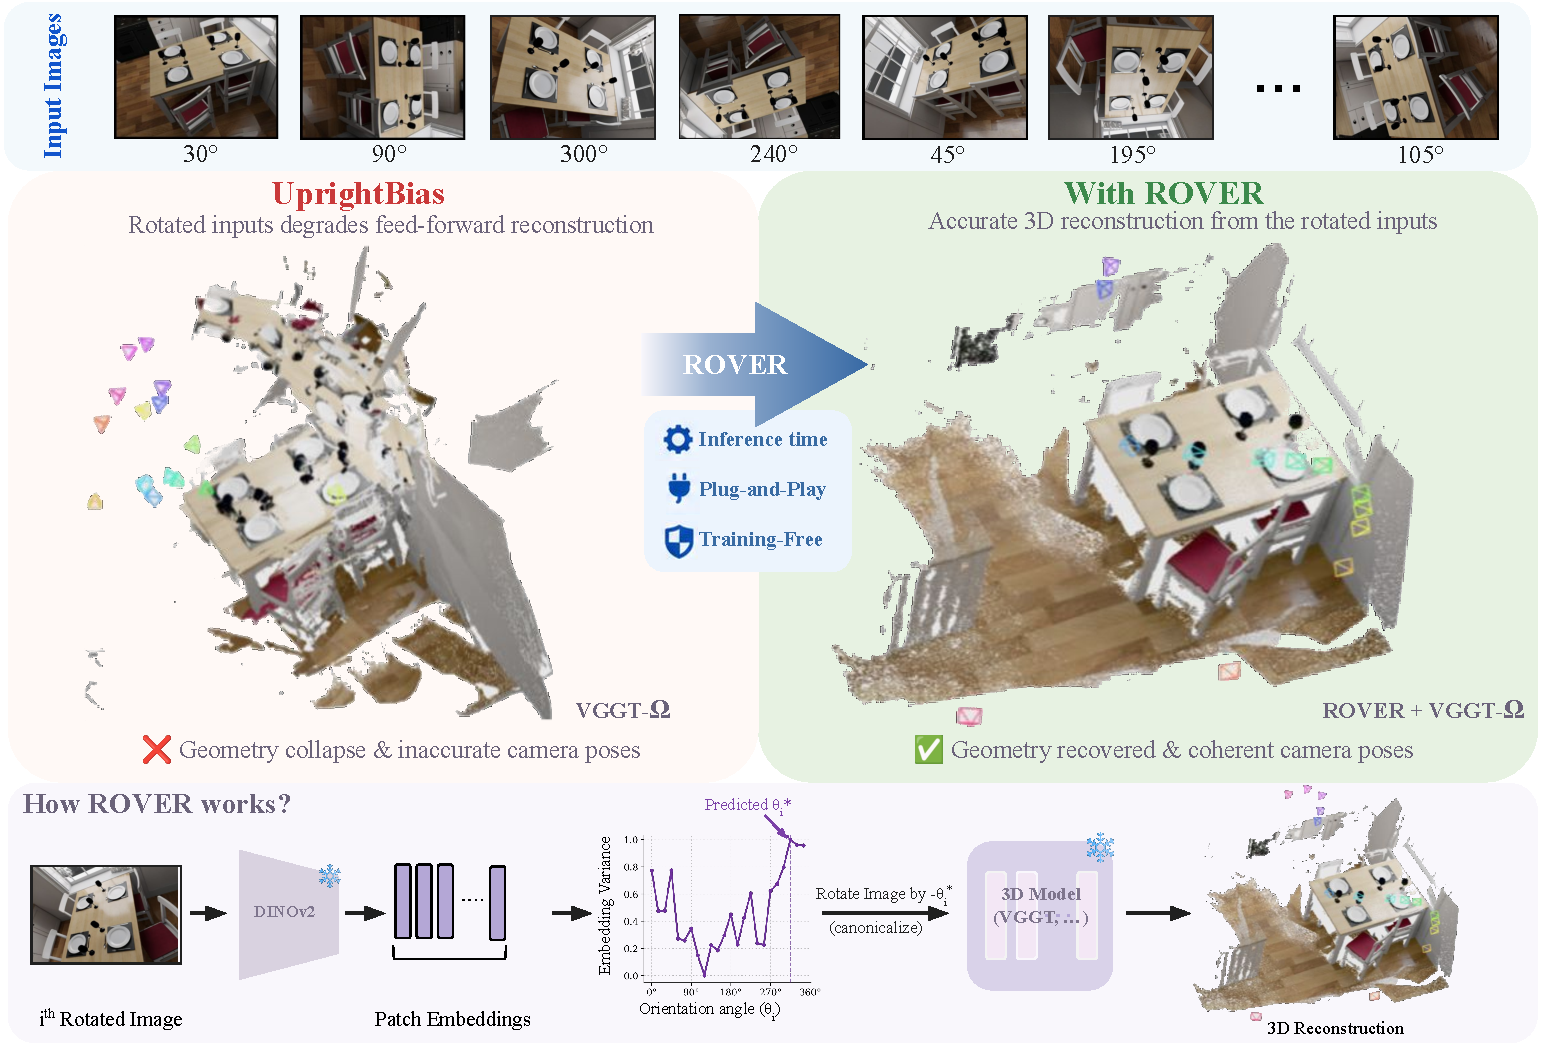
\includegraphics[width=0.85\linewidth]{Figures/Teaser/Teaser.pdf}
    \caption{\textbf{Robust 3D reconstruction under image rotations with ROVER.} Feeds of arbitrarily rotated images (top) cause standard feed-forward 3D models (e.g., VGGT-$\Omega$) to suffer from geometry collapse due to an implicit upright bias (left). Our training-free, plug-and-play module, ROVER, leverages feature properties in frozen DINOv2 to predict and canonicalize image orientation at inference time (bottom), recovering accurate 3D geometry and coherent camera poses (right).
    }
    \vspace{1em}
    \label{fig:teaser}
\end{figure}


\vspace{-3mm}
\begin{abstract}
We uncover a largely overlooked vulnerability in feed forward reconstruction models: sensitivity to image orientation.
Across state-of-the-art architectures rotational perturbations of input images cause severe degradation in both camera pose estimation and point-map quality.
We term this failure mode UprightBias and trace its origin to a near-universal upright orientation of training corpora, which causes models to implicitly assume canonically upright inputs at inference time.
We find that patch-level embedding variance from a DINOv2 encoder provides a reliable zero-shot signal for identifying the canonical upright orientation.
Leveraging this insight, we introduce \textbf{ROVER} (\textbf{RO}tation estimation via \textbf{V}ariance-based \textbf{E}mbedding \textbf{R}ectification), a training-free framework that estimates and rectifies image orientation at inference, leaving all downstream model weights unchanged.
For evaluation, we introduce a Controlled Rotation Synthesis protocol that generates rotated views from upright images. 
We also curate \textbf{RotMV} (\textbf{Rot}ational \textbf{M}ulti-\textbf{V}iew), which, to the best of our knowledge, is the first benchmark of paired upright and real-world rotated multi-view sequences captured from fixed viewpoints.
Experiments across the datasets demonstrate that ROVER consistently shows improvements, reducing pose estimation errors upto 80\% and point-map estimation errors by over 58\% on average.
%%% Important note about the metrics average of 59% completeness (metric) on 3 datasets 7 scenes NRGBD and RotMV 
%%% 
% We then investigate whether it can be resolved without modifying or retraining existing models.
% We discover that patch-level embeddings of a frozen DINOv2 encoder exhibit maximal spatial variance at the canonical upright orientation of an image making embedding variance a zero-shot proxy for image uprightness.
% For evaluation, we introduce a Controlled Rotation Synthesis protocol and curate \textbf{RotMV}(\textbf{Rot}ational \textbf{M}ulti-\textbf{V}iew), the first benchmark of paired upright and real-world rotated multi-view sequences captured from fixed viewpoints.
% Experiments across seven datasets demonstrate that ROVER consistently restores camera pose accuracy and point-map quality under arbitrary rotations, outperforming all evaluated baselines.
\end{abstract}
\section{Introduction}
Feed-forward multi-view reconstruction models \citep{wang2025vggt, wang2025pi, depthanything3, wang2026vggtomega, dust3r_cvpr24} regress camera poses and dense geometry directly, without the iterative correspondence-based estimation used by classical structure-from-motion (SfM) \citep{structurefrommotion1, structurefrommotion2, structurefrommotion3}. Their strong performance on standard multi-view benchmarks, however, does not necessarily translate to robustness under the diverse conditions encountered in real-world image capture \citep{liu2026realx3d}. One such source of variability is camera orientation, which can vary substantially across handheld photography, egocentric video capture, and other settings with unconstrained camera motion \citep{xian2019uprightnet}. Classical SfM pipelines are inherently robust to such changes because their geometric estimation relies on rotation invariant image features \citep{SIFTpaper}. For feed-forward reconstruction models, however, robustness to camera orientation is generally assumed as an inherent property of the reconstruction task.

We put this assumption to the test by asking a simple question: \emph{How robust are modern feed-forward reconstruction models to changes in image orientation?} 
A well-behaved reconstruction model should produce point clouds invariant to such changes, while camera poses should transform equivariantly.
Surprisingly, we find that applying random planar rotations on subset of input images leads to degradation in camera pose estimation and dense reconstruction across state-of-the-art (SOTA) feed-forward models. 
We observe this degradation across VGGT \citep{wang2025vggt}, VGGT-$\Omega$ \citep{wang2026vggtomega}, $\pi^3$ \citep{wang2025pi}, MapAnything (MapA.) \citep{keetha2026mapanything} and Depth Anything 3 (DA3) \citep{depthanything3}, while classical SfM with COLMAP \citep{colmap} remains robust to the same perturbations.
Quantitatively, \Cref{fig:baseline_performance}(a) shows that both Absolute Trajectory Error (ATE) and Relative Pose Error (RPE) increase with the number of rotated input images across the feed-forward models. The corresponding qualitative degradation in reconstructed geometry is shown in \Cref{fig:baseline_performance}(b)
We further investigate the extent of this orientation sensitivity across rotations about all three axes (roll, pitch, and yaw) in \cref{sec:how_severe_is_upright_bias}.

We refer to this sensitivity to camera orientation as \emph{UprightBias}: the tendency of feed-forward reconstruction models to perform substantially better on images presented in a canonical upright orientation. The effect is particularly striking because it persists across architecturally diverse models, including reference-view attention networks (VGGT, VGGT-$\Omega$), reference-free permutation-equivariant approaches ($\boldsymbol{\pi^3}$), generalized multi-view matchers such as MapA. and DA3.
% This behavior is particularly striking because it persists across substantially different architectural designs, including reference-view attention models (VGGT, VGGT-$\Omega$), reference-free permutation-equivariant networks ($\boldsymbol{\pi^3}$), and generalized multi-view matchers such as MapAnything (MapA.) \citep{keetha2026mapanything} and DA3. 
% Given how different these designs are from one another, the shared sensitivity is unlikely to stem from any common architectural inductive bias; however,
% Despite the differences, these models exhibit similar sensitivity to image orientation, suggesting that it is unlikely to arise from architectural inductive bias.
Notably, however, each of these models relies on large-scale 3D reconstruction datasets which predominantly consists of canonically-upright images, and models trained on such image sets may potentially learn orientation-specific regularities instead of generalizing across arbitrary rotations.
% -orientation which raises the possibility that the training-data distribution contributes to this behavior. In particular, models may learn orientation-specific regularities prevalent in predominantly canonical training images, rather than developing robustness to arbitrary image rotations.
We investigate this hypothesis through an audit of the training data used by these models in ~\cref{ssec:data_audit}, which shows that an overwhelming majority of these datasets consist of images that are upright by construction, spanning indoor RGB-D benchmarks, outdoor photo collections, and a range of other sources. 

One natural remedy to fix the Upright Bias would be to rebalance the training data with rotated multi-view images and corresponding geometric annotations \citep{redistributingtrainingdata1, tang2022invarianttrainingdata2, kang2019decouplingtrainingdata3}; however, these feed-forward models are built on pretrained visual backbones like DINO-v2/v3 \citep{oquab2023dinov2, simeoni2025dinov3}, and fine-tuning on a rotation-heavy distribution shifts the backbone away from its pretraining regime, which is known to distort learned representations, even when the fine-tuning objective is otherwise met \citep{kumar2022finetuningchallenges, tang2020longchallenges, kang2019decouplingtrainingdata3, horizontalprior}. Further, despite both DA3 and VGGT-$\Omega$ employing $90^\circ$ rotation augmentation in their training pipeline, yet, as shown in \Cref{fig:baseline_performance}(a), they \textit{still exhibit} substantial degradation under arbitrarily-rotated inputs. For instance, we observe that a simple fine-tuning of $\pi^3$ on arbitrarily-rotated training images yields not just inconsistent but often degraded performance (see \cref{sec:training_data_rebalancing} of the supplementary), further suggesting that rebalancing the training distribution \textit{alone} is insufficient to eliminate the upright bias. 
% To probe this further, we fine-tune \textbf{$\pi^3$} on arbitrarily-rotated input images, with results reported in the supplementary \cref{sec:training_data_rebalancing}.
% The resulting model shows inconsistent and often degraded performance under rotated inputs, suggesting that retraining with rotated data alone is insufficient to eliminate this bias.
% Notably, both DA3 and VGGT-$\Omega$ incorporate $90^\circ$ rotation augmentation during training, yet still exhibit substantial degradation under rotated inputs, directly demonstrating that augmentation alone is insufficient to resolve \textcolor{green}{[Abhipsa: is calling it like a proper noun always necessary? :P ]}UprightBias. 
% We empirically validate these limitations further in the supplementary \cref{sec:training_data_rebalancing}, where fine-tuning $\pi^3$ on rotated data confirms inconsistent, often degraded performance rather than resolving UprightBias.
Lastly, we note that retraining large-scale feed-forward models requires \textit{paired} rotated multi-view data with ground-truth geometry, which is currently missing in the existing benchmarks. 

\begin{figure}[t]
    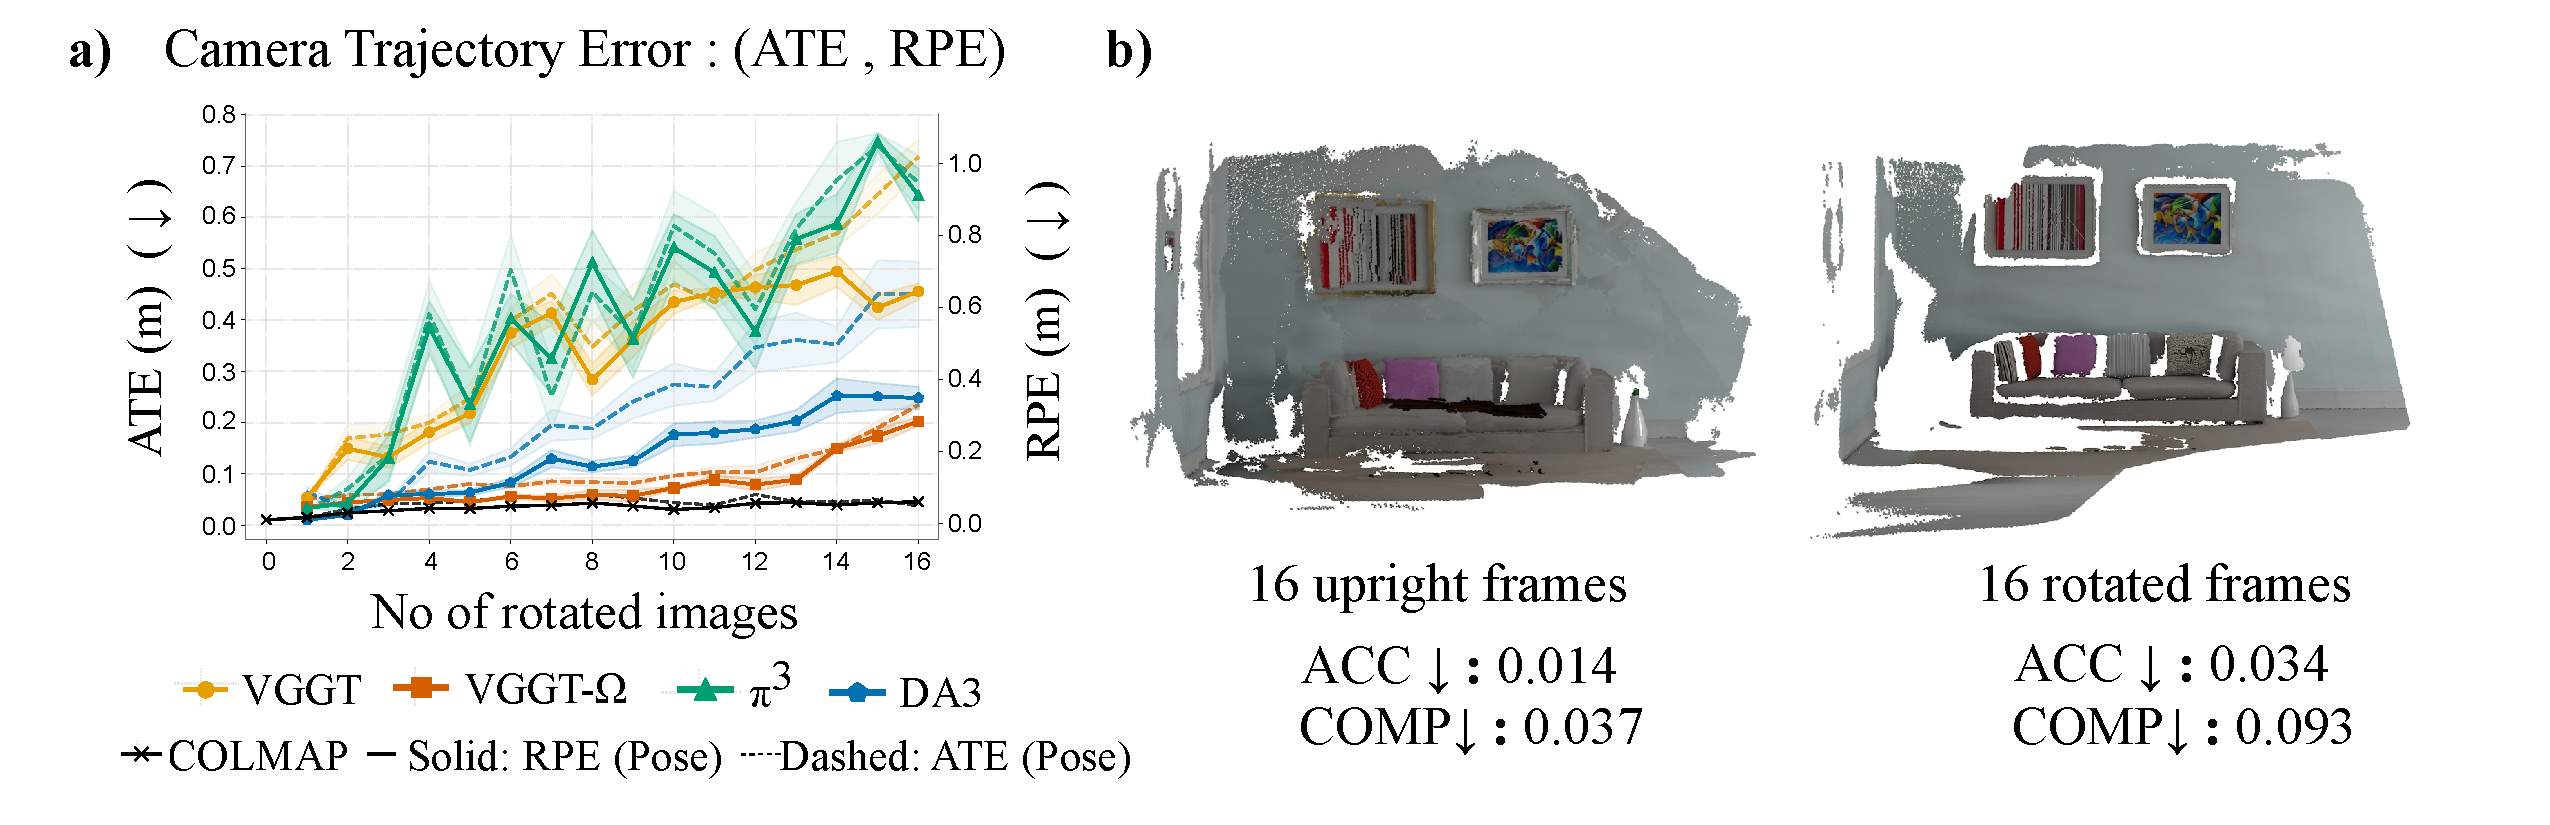
\includegraphics[width=\linewidth]{Figures/fig2/fig2.pdf}
    \caption{\textbf{Robustness against in-plane rotations:}
    (a) Camera poses error increases as number of rotated input images increases ($\theta \sim \mathcal{U}(0^\circ, 360^\circ)$). (b) Qualitative 3D reconstruction degradation on VGGT-$\Omega$ when introducing 16 rotated images sampled from $\theta \sim \mathcal{U}(0^\circ, 360^\circ)$.}
    \label{fig:baseline_performance}
    \vspace{-3mm}
\end{figure}

Rather than adapting a reconstruction model to rotated inputs, we instead ask whether the inputs \textit{themselves} can be rectified to the canonical orientation before reconstruction.
This requires a visual representation that can provide a reliable signal of image orientation without rotation labels or model retraining. To this end, we find that DINOv2 token embeddings exhibit \textit{systematic orientation-dependent variation}, which can be leveraged to enable zero-shot rectification by identifying the orientation that maximizes feature variance. Building on this observation, we propose \textbf{ROVER} (\textbf{RO}tation estimation via \textbf{V}ariance-based \textbf{E}mbedding \textbf{R}ectification), a lightweight \textit{training-free} framework that operates at inference time in a plug-and-play manner with any encoder, as illustrated in ~\cref{fig:teaser}.
% \sout{Along with this, we also introduce \textbf{RotMV} (\textbf{Rot}ational \textbf{M}ulti-\textbf{V}iew), an evaluation benchmark comprising multi-view sequences captured at systematically varied camera orientations to assess rotation-invariance of feed-forward models under real-world scene conditions} \textcolor{red}{[Priyam: any specifics of the benchmark?]}.
Along with this, we introduce \textbf{RotMV} (\textbf{Rot}ational \textbf{M}ulti-\textbf{V}iew), a real-world benchmark comprising of seven multi-view sequences captured across $16$ viewpoints and $12$ in-plane camera orientations spanning $360^\circ$, enabling systematic evaluation of rotation-invariance in feed-forward models.
Extensive Experiments on 7-Scenes, NRGB-D, DTU, ETH3D, Mip-NeRF 360, Tanks \& Temples and RotMV, shows that ROVER recovers reconstruction quality under arbitrary planar rotations while preserving performance on canonical inputs.
% To enable such a training-free approach, we seek a visual representation that provides information about image orientation and can therefore serve as a signal for estimating the canonical orientation of the input.
% We find that DINOv2 token embeddings exhibit a strong orientation signal, with feature variance maximized at the canonical orientation, enabling zero-shot orientation estimation without prior knowledge of the applied rotations or model retraining.
% Leveraging this observation, we propose \textcolor{orange}{[Priyam: I'm not sure if we need to bold ROVER, as well as de-acronymize it here, although it's a choice of writing taste]} \textbf{ROVER} (\textbf{RO}tation estimation via \textbf{V}ariance-based \textbf{E}mbedding \textbf{R}ectification), a lightweight training-free framework that canonicalizes rotated inputs before reconstruction. 
% \textcolor{orange}{[Priyam: This line of RotMV (please give a better name) disconnects with the prev. para about no dataset existing for rotated imgs with geometry info]} \textcolor{green}{[Abhipsa: I feel this line's construction could be improved. Like to the best of our knowledge, we are the first to introduce..., also make it clear that it is an eval dataset]} Since no existing benchmark provides paired upright and rotated multi-view sequences under real-world capture conditions, we introduce \textbf{RotMV}, a curated dataset of real-world multi-view sequences with systematically varied orientations to support controlled evaluation of rotation robustness. Extensive experiments show that ROVER consistently recovers 3D reconstruction quality under arbitrary planar rotations while preserving performance on canonical inputs.
In summary, our main contributions are:

$\bullet$ We identify a previously uncharacterized sensitivity to image orientation in state-of-the-art feed-forward 3D reconstruction models, a phenomenon we term UprightBias, and show that it is systemic across diverse model architectures and families.

$\bullet$ To address it, we propose ROVER -- a lightweight, training-free framework that rectifies input rotations at inference time using orientation-dependent variance in DINOv2 embeddings.

% $\bullet$ \textcolor{orange}{[Priyam: This contribution is currently in a very bad shape (writing-wise). Also check the natural order of the contributions, if they make sense in the current ordering in which they're mentioned]} \Badri{Proper motivation of introducing RotMV is missing, we should use "controlled rotation synthesis" as synthetic and need real data} 
% \textcolor{blue}{We extensively evaluate rotation robustness across six existing datasets through controlled rotation synthesis. Furthermore, we introduce \textbf{RotMV}, a real-world benchmark with paired upright and rotated multi-view sequences, to further validate our findings under real-world camera rotations.}

$\bullet$ Across six existing multi-view datasets, we conduct a systematic assessment of rotation-invariance of various feed-forward models under controlled rotation synthesis, isolating the effect of camera orientation on reconstruction.

$\bullet$ To complement synthetic evaluation with real-world data, we introduce RotMV, a benchmark comprising paired upright and rotated multi-view sequences captured under systematically varied camera orientations.

\section{Related Work}

\textbf{Robustness and Bias in Vision Models:}
Although modern deep learning models encode overrepresented training patterns as implicit priors, these task-extrinsic biases often remain hidden under standard benchmarks until those assumptions are violated.
Extensive work has demonstrated this across visual recognition, including biases toward texture over shape, shortcut correlations, photographer preferences, object position, and background context~\citep{geirhos2018imagenet, geirhos2020shortcut, torralba2011unbiased, xiao2020noise, liu2026optigeoefficientmonoculargeometry}.
These findings have motivated robustness benchmarks beyond clean in-distribution accuracy~\citep{hendrycks2019benchmarking} and approaches based on architectural inductive biases or inference-time adaptation~\citep{cohen2016group, weiler2019general, sun2020test, wang2020tent}.
Despite this extensive literature, robustness has been studied primarily in recognition tasks such as classification, segmentation, and detection. 
In single-image geometry, prior studies have identified specific camera pose and spatial distribution biases in depth estimation ~\citep{vandijk2019neuralnetworksdepthsingle, zhao2021cameraposemattersimproving}, while recent work highlights broader viewpoint instabilities in vision foundation models~\citep{michalkiewicz2024viewscreatedequalanalyzing}. Similarly, \cite{jiang2025youviewpointinvariant} investigates viewpoint invariance in policy learning.
However, whether similar priors arise in feed-forward geometric foundation models remains largely unexplored.

\textbf{Image Orientation and Uprightness Estimation:}
The resulting sensitivity to image orientation naturally raises the question of whether canonical upright orientation can be estimated reliably at inference time.
Existing approaches include geometric methods based on line classification~\citep{ctrlc, lee2021ctrl}, feature matching \citep{nordstrom2026whohandlesorientationcvpr, nordstrom2026lomawhohandlesorientationeccv} and learning-based methods such as UprightNet~\citep{xian2019uprightnet}, which predicts 2-DoF camera orientation from indoor surface normals, and GeoCalib~\citep{veicht2024geocalib}, which jointly estimates camera intrinsics and gravity direction through differentiable geometric optimization.
Inference-time canonicalization offers an alternative for robustness under distribution shifts. 
FOCAL~\citep{singhal2025testtimeimageCanonicalization} searches for a canonical input transformation using test time optimization of likelihoods with foundation-model, while G3TUP!~\citep{kani2026g3t} fine-tunes VGGT to produce upright point clouds. 

In contrast, we identify upright bias as a previously unrecognized failure mode shared across modern feed-forward reconstruction models and introduce ROVER, a Plug-and-Play inference-time canonicalization framework that estimates orientation using DINOv2, requiring neither scene-specific geometric structure nor model retraining and generalizing across indoor and outdoor scenes.

% {\color{blue}
% \begin{enumerate}

%     \item \textbf{How Do Neural Networks See Depth in Single Images?}~\citep{vandijk2019neuralnetworksdepthsingle} --- 
%     \textit{Tom van Dijk, Guido C. H. E. de Croon} --- \textbf{ICCV 2019}.  
%     The paper finds that MonoDepth relies strongly on an object's \textbf{vertical image position} rather than apparent size for depth estimation. Because this cue depends on camera pose, changes in pitch can lead to systematic depth errors.

%     \item \textbf{Camera Pose Matters: Improving Depth Prediction by Mitigating Pose Distribution Bias}~\citep{zhao2021cameraposemattersimproving} --- 
%     \textit{Yunhan Zhao, Shu Kong, Charless Fowlkes} --- \textbf{CVPR 2021}.  
%     The authors identify a \textbf{camera-pose distribution bias} in monocular depth estimation, where models become unreliable on uncommon or unseen viewpoints. They mitigate this using perspective-aware augmentation and explicit camera-pose conditioning.

%     % \item \textbf{Breaking the Horizontal Prior: From Long-Tailed Orientation Bias to Roll-Robust Monocular Depth Estimation}~\citep{tang2026breakinghorizontalpriorlongtailed} --- 
%     % \textit{Kaihua Tang et al.} --- \textbf{2026}.  
%     % This work identifies a \textbf{Horizontal Prior} caused by the dominance of upright images in monocular depth training data, leading to degradation under camera roll. The authors propose an Invariant Depth Constraint to learn more rotation-stable representations.

%     \item \textbf{AerialMegaDepth: Learning Aerial-Ground Reconstruction and View Synthesis}~\citep{vuong2025aerialmegadepthlearningaerialgroundreconstruction} --- 
%     \textit{Khiem Vuong, Anurag Ghosh, Deva Ramanan, Srinivasa Narasimhan, Shubham Tulsiani} --- \textbf{CVPR 2025}.  
%     The paper shows that learned 3D reconstruction struggles under \textbf{extreme aerial-ground viewpoint changes}, partly due to insufficient viewpoint diversity in training data. Fine-tuning on a dedicated aerial-ground corpus substantially improves camera estimation and registration.


%     \item \textbf{Not All Views are Created Equal: Analyzing Viewpoint Instabilities in Vision Foundation Models}~\citep{michalkiewicz2024viewscreatedequalanalyzing} --- 
%     \textit{Mateusz Michalkiewicz et al.} --- \textbf{ICCV 2025}.  
%     The paper analyzes \textbf{viewpoint instability} in foundation models and shows that representation quality can vary significantly with viewing angle. These instabilities also affect downstream 3D reasoning and reconstruction tasks.

%     \item \textbf{OptiGeo: Efficient Monocular Geometry for Embodied Perception in Optically Challenging Scenes}~\citep{liu2026optigeoefficientmonoculargeometry} --- 
%     \textit{Muxin Liu et al.} --- \textbf{2026}.  
%     OptiGeo shows that failures on transparent and reflective surfaces can arise from \textbf{biased real-depth supervision}, where sensor errors are inherited by learned geometry models. It mitigates this by replacing unreliable supervision with clean-geometry teacher and residual-trimmed alignment.

% \end{enumerate}
% }
\vspace{-2mm}
\section{Method}
\label{sec:method}

\textbf{Problem Setup:}
Let $\mathcal{F}$ denote a pre-trained feed-forward multi-view reconstruction model that maps a set of $N$ multi-view images to camera pose and dense geometric predictions. Given a set of input images $\mathcal{I}^R =\{ \mathbf{I}^{\theta_i}_i \}_{i=1}^N$ where each view $\mathbf{I}_i^{\theta_i}$ is captured at an arbitrary in-plane orientation $\theta_i \in [0^\circ, 360^\circ)$. 
Our goal is to recover a scene representation $\hat{\mathcal{G}}$ comparable in quality to that obtained from canonically upright inputs, without retraining or modifying $\mathcal{F}$.

Existing multi-view benchmarks lack systematically rotated images with corresponding ground-truth annotations, making it difficult to evaluate robustness to arbitrary camera orientations.
We therefore develop a Controlled Rotation Synthesis, a procedure that generates rotated multi-view inputs while preserving the underlying scene geometry and avoiding rotation-induced artifacts.
The proposed procedure enables synthetic rotations about all three axes (roll, pitch, and yaw), while avoiding rotation-induced artifacts.
To complement the synthetically rotated benchmarks, we construct RotMV, a real-world benchmark comprising multiple scenes, with each scene containing multi-view images captured at multiple camera orientations for every viewpoint.
% We analyze the performance of ROVER across both types of benchmarks for pointmap reconstruction and camera pose estimation.
In this section, we discuss the controlled rotation synthesis procedure in \cref{sec:rendering_based_rotation} and our proposed method for correcting UprightBias in \cref{sec:ROVER_detail}.

\subsection{Controlled Rotation Synthesis}
\label{sec:rendering_based_rotation}

Our goal is to generate synthetic views by isolating the effect of camera orientation only. 
The created rotation should alter only the camera pose while leaving the scene content and image formation otherwise unchanged.
This is not possible if we naively rotate the images in image space, because it introduces various artifacts like padding, cropping, and resolution changes, as illustrated in \Cref{fig:bicycle_rot}.


Given an upright multi-view sequence $\mathcal I$, we first reconstruct its 3D scene representation $\mathcal G_{\mathrm{3DGS}}$ and corresponding camera poses using a 3D Gaussian Splatting\citep{kerbl3Dgaussians}.
For each view $i$, let its original camera pose be $\mathbf P_i=[\mathbf R_i\mid\mathbf t_i]$, where $\mathbf R_i$ and $\mathbf t_i$ denote the camera rotation and translation, respectively following camera to world convention.
For a synthetic in-plane rotation of $\theta$, represented by $\mathbf R_z(\theta) \in \mathrm{SO}(3)$, the corresponding camera pose is given by $\mathbf P_i^{\theta}=\left[\mathbf R_i\mathbf R_z(\theta)\;\middle|\;\mathbf t_i\right]$.
Analogously, pitch and yaw rotations are synthesized by replacing $\mathbf R_z(\theta)$ with $\mathbf R_x(\theta)$ and $\mathbf R_y(\theta)$, respectively.
The corresponding view is then rendered as:
$$
\tilde{\mathbf I}_i^{\theta_i}=\operatorname{Render}(\mathcal G_{\mathrm{3DGS}},\mathbf P_i^{\theta_i}).$$
The fidelity of $\tilde{\mathbf I}_i^{\theta_i}$ depends on the quality of the reconstructed $\mathcal G_{\mathrm{3DGS}}$, which may vary with the input views and rotation angle $\theta$.
To improve it, we further refine $\mathcal G_{\mathrm{3DGS}}$ using DiFix3D+\citep{wu2025difix3d} Denoiser, and then render the rotated views to obtain the final $\mathbf I_i^{\theta_i}$.
Low-quality renders may still occur and are discarded using a two-stage filtering pipeline \citep{wu2026visualquality}, detailed in the supplementary \cref{sec:image_statistics}. 
Full pipeline details are included in supplementary, specifically the rendering algorithm in \cref{sec:algorithm}, quality filtering procedure and dataset statistics in \cref{sec:image_statistics}.

% \clearpage
\subsection{ROVER}
\label{sec:ROVER_detail}

\begin{wrapfigure}{r}{0.5\textwidth} 
    \vspace{-2em} 
    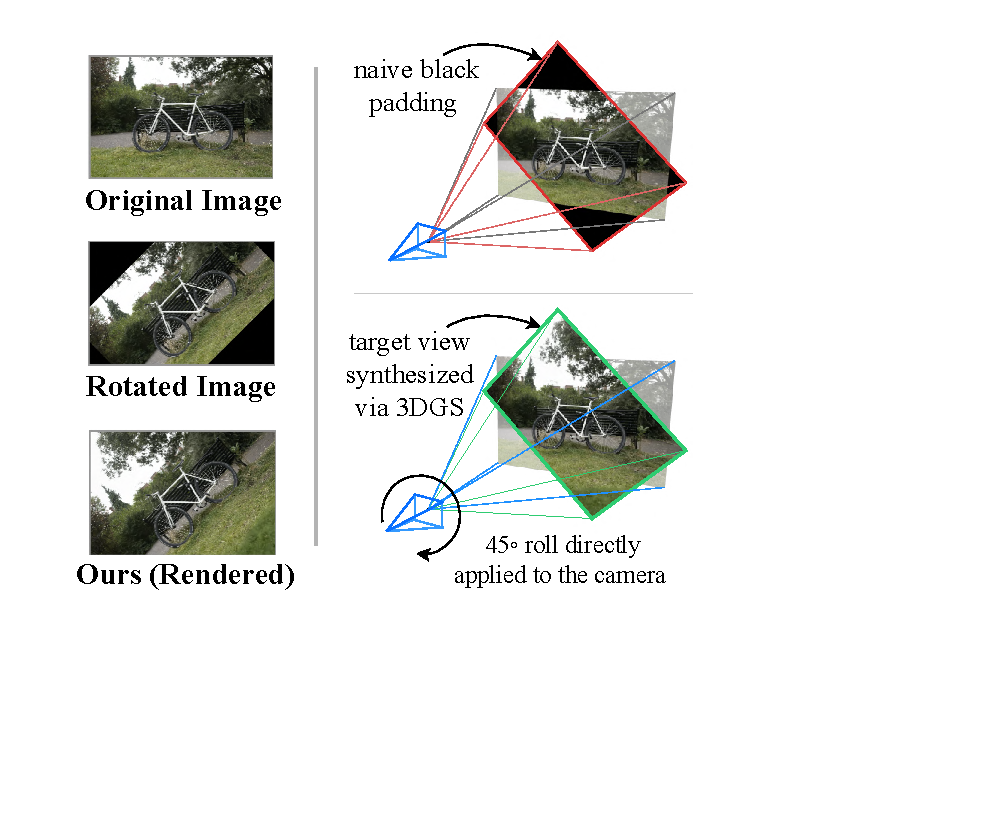
\includegraphics[width=\linewidth]{Figures/fig3/fig3.pdf}
    \caption{\textbf{Controlled Rotation Synthesis.} Naive 2D image rotation (\emph{top right}) introduces black padding, cropping artifacts, or resolution shifts. In contrast, our approach (\emph{bottom right}) applies planar roll $\mathbf{R}_z(\theta)$ directly to the camera pose and synthesizes the target view via 3DGS, generating naturally rotated images.}
    \label{fig:bicycle_rot}
    \vspace{-1em}
\end{wrapfigure}
ROVER constructs a canonicalization operator $T$ that maps an arbitrarily oriented input sequence to the canonical upright orientation expected by the pre-trained reconstruction model.
Our method realizes the canonicalization operator $T$ by decomposing it into two sequential operators, $T=C\circ E$, where $E:\mathcal{I}^R\rightarrow\hat{\Theta}$ estimates the canonical orientation of each image in the input sequence, with $\hat{\Theta}=\{\hat{\theta}_i\}_{i=1}^{N}$ denoting the estimated orientations, and $C:(\mathcal{I},\hat{\Theta})\rightarrow\mathcal{I}^{\mathrm{can}}$ applies the corresponding transformations to produce the canonicalized image sequence. 
Since both operators act entirely in image space, ROVER requires neither retraining nor architectural modifications to the underlying feed-forward reconstruction model.

% \textbf{Estimating the Canonical Orientation:}

% The orientation estimation operator $E$ determines the canonical 
% orientation of each image in the input sequence. To implement $E$, 
% we require a representation whose feature geometry varies 
% predictably with image orientation. We use a frozen DINOv2 
% encoder $\phi$ \citep{oquab2023dinov2}, motivated by an empirical 
% observation established in the supplementary: patch-level embeddings 
% from DINOv2 exhibit maximal spatial variance when the input image 
% is presented in its canonical upright orientation. We attribute 
% this to the KoLeo regularizer \citep{sablayrolles2018spreadingkoleoregularizer} 
% used during DINOv2 training, which explicitly encourages uniform 
% dispersion of patch embeddings, thereby inducing an 
% orientation-sensitive structure in the representation space.

% For each input image $\mathbf{I}$ and candidate orientation $\theta \in \Theta$, we obtain patch embeddings $\mathbf{Z}_{\theta} = \phi(\mathbf{I}^{\theta}) = \{\mathbf{z}_j^\theta\}_{j=1}^M$, $\mathbf{z}_j^\theta \in \mathbb{R}^D$, and estimate the canonical orientation as:
% %
% \begin{equation}
% V(\theta) = \frac{1}{M}\sum_{j=1}^{M}
% \left\|\mathbf{z}_j^\theta - \bar{\mathbf{z}}^\theta\right\|_2^2,
% \qquad
% E(\mathbf{I}) = \arg\max_{\theta \in \Theta}\, V(\theta),
% \end{equation}
% where $\bar{\mathbf{z}}^\theta = \frac{1}{M}\sum_{j=1}^{M} 
% \mathbf{z}_j^\theta$.

% To achieve $1^\circ$ resolution while avoiding exhaustive 
% evaluation over all $360$ candidates, we employ a 
% coarse-to-fine search. We first evaluate $V(\theta)$ over 
% a coarse grid $\Theta_\text{coarse} = \{15^\circ \times k 
% \mid k = 1, \ldots, 24\}$, obtaining a coarse estimate 
% $\theta_c = \arg\max_{\theta \in \Theta_\text{coarse}} V(\theta)$. 
% We then refine within $[\theta_c - 7^\circ, \theta_c + 7^\circ]$ 
% at $1^\circ$ intervals. 

% \textbf{Applying the Canonicalization Operator:}
% Given the estimated orientation $\hat{\theta}=E(\mathbf{I})$, the canonicalization operator $C$ restores the input image to its canonical orientation by rotating it using the estimated correction angle.
% Formally, the canonicalized image is obtained as $\mathbf{I}^{\mathrm{can}}\approx\mathrm{R}_z(\mathbf{I},\hat{\theta})$, where the approximation reflects that $\hat{\theta}$ is estimated with finite angular resolution.
% Applying $C$ independently to every image in the input sequence produces the canonicalized image sequence $\mathcal{I}^{\mathrm{can}}=\{\mathbf{I}_i^{\mathrm{can}}\}_{i=1}^{N}$, which is then provided directly to the original feed-forward reconstruction model for scene reconstruction without retraining or modifying its architecture.


% Given the estimated orientation $\hat{\theta} = E(\mathbf{I})$, 
% the canonicalization operator $C$ restores the image to its 
% canonical upright orientation by applying a corrective in-plane 
% rotation $ \mathbf{I}^{\mathrm{can}} = C(\mathbf{I}) = \mathbf{I}^{-\hat{\theta}}$ where $\mathbf{I}^{-\hat{\theta}}$ denotes the image rotated 
% by $-\hat{\theta}$, correcting for the estimated deviation 
% from the canonical orientation. Applying $C$ independently 
% to every image in the input sequence yields the canonicalized 
% sequence $\mathcal{I}^{\mathrm{can}} = 
% \{\mathbf{I}_i^{\mathrm{can}}\}_{i=1}^{N}$, which is passed 
% directly to $\mathcal{F}$ for scene reconstruction without 
% any retraining or architectural modification.

% \AD{@Badri Please re-write this section. What is that key insight which led us to go with the variance based method. 1.) Produce some $V(\theta)$ plots for different rotations. 2.) Also, describe the method using algorithm. 3.) Fix the notations for rotation, upright set, rotated set, candidate angles etc. thorughout the manuscript. Best way to structure this section: Observation, Score computation, Method, RUn-time analysis. }

% We observe that (validated in the supplementary): the final layer patch-level embeddings of a 
% frozen DINOv2 encoder $\phi$ \citep{oquab2023dinov2} exhibit 
% maximal spatial variance when the input image is presented in its canonical upright orientation, and this variance is lower as the image deviates from upright. We attribute this to the KoLeo regularizer \citep{sablayrolles2018spreadingkoleoregularizer} used during DINOv2 training, which explicitly encourages uniform dispersion of patch embeddings. Since natural upright images dominate the pretraining distribution, the encoder implicitly learns representations that are most dispersed for canonical orientations, making patch embedding variance a reliable proxy for image uprightness. Variance plots across datasets and scenes, confirming that DINOv2 patch embedding variance peaks at the canonical upright orientation, are provided in supplementary \cref{sec:ROVER_empirical_plots}.
\textbf{Estimating the Canonical Orientation:}
We made an important observation that enabled us to estimate orientation directly from the representations of DINOv2 encoder.
DINOv2 employs the KoLeo regularizer \citep{sablayrolles2018spreadingkoleoregularizer}, which encourages uniform dispersion of the learned embeddings.
This provides a natural basis for measuring the spatial variance of its patch-level embeddings.
Since the DINOv2 pretraining distribution is dominated by naturally upright images, we hypothesize that this dispersion is strongest when an image is presented in its canonical upright orientation.
We observe that the spatial variance of final-layer patch embeddings indeed peaks at the canonical upright orientation and decreases as the image deviates from upright, consistently across datasets and scenes (provided in supplementary \cref{sec:ROVER_empirical_plots}).
This makes patch embedding variance a reliable proxy for image uprightness, allowing us to estimate the canonical orientation by maximizing the variance over candidate orientations.
For each input image $\mathbf{I}$ and candidate orientation $\theta \in \Theta$, we compute the DINOv2 patch embeddings $\mathbf{Z}^{\theta}=\phi(\mathbf{I}^{\theta})=\{\mathbf{z}_j^\theta\}_{j=1}^{M}$ with mean embedding $\bar{\mathbf{z}}^\theta$, and estimate the canonical orientation $\hat{\theta}$ by maximizing their spatial variance:
\begin{equation*}
V(\theta) = \frac{1}{M}\sum_{j=1}^{M}
\left\|\mathbf{z}_j^\theta - \bar{\mathbf{z}}^\theta\right\|_2^2
\quad\Longrightarrow\quad
E(\mathbf{I}) = \hat{\theta} = \arg\max_{\theta \in \Theta} V(\theta).
\end{equation*}
\vspace{-2mm}

% For each input image $\mathbf{I}$ and candidate orientation 
% $\theta \in \Theta$, we rotate the image by $\theta$ and pass 
% it through the frozen DINOv2 encoder to obtain patch embeddings 
% $\mathbf{Z}_{\theta} = \phi(\mathbf{I}^{\theta}) = 
% \{\mathbf{z}_j^\theta\}_{j=1}^M$. 
% The orientation score $V(\theta)$ is defined as 
% the spatial variance of these embeddings:
% \begin{equation}
% V(\theta) = \frac{1}{M}\sum_{j=1}^{M}
% \left\|\mathbf{z}_j^\theta - \bar{\mathbf{z}}^\theta\right\|_2^2,
% \qquad
% E(\mathbf{I}) = \hat{\theta} = \arg\max_{\theta \in \Theta}\, V(\theta).
% \end{equation}
% where $\bar{\mathbf{z}}^\theta = \frac{1}{M}\sum_{j=1}^{M}\mathbf{z}_j^\theta$ and the orientation estimation operator $E$ selects the candidate 
% orientation that maximizes the variance score.

\textbf{Applying the Canonicalization Operator:}
Given $\hat{\theta}$, the canonicalization operator $C$ applies a corrective rotation to restore the image to its upright orientation $\mathbf{I}^{\mathrm{can}} = C(\mathbf{I}) = \mathbf{I}^{-\hat{\theta}}$. Applying $T = C \circ E$ independently to every image in $\mathcal{I}^R$ yields the canonicalized sequence $\mathcal{I}^{\mathrm{can}} = \{\mathbf{I}_i^{\mathrm{can}}\}_{i=1}^{N}$, which is passed to feed-forward model $\mathcal{F}$.
Exhaustive evaluation of $V(\theta)$ over all $360$ integer-degree candidates requires $360$ DINOv2 forward passes per image. 
We instead employ a coarse-to-fine search that requires only two batched DINOv2 forward passes per multi-view sequence at inference time. 
In the coarse stage, we evaluate $V(\theta)$ over $\Theta_\text{coarse} = \{15^\circ \times k \mid k = 1, \ldots, 24\}$ and obtain $\theta_c = \arg\max_{\theta \in \Theta_\text{coarse}} V(\theta)$.
In the fine stage, we evaluate $V(\theta)$ within $[\theta_c - 7^\circ,\, \theta_c + 7^\circ]$ at $1^\circ$ intervals.
Since all candidate rotations for a stage can be batched, each stage requires only a one DINOv2 forward pass for the entire multi-view sequence. We include results for latency in \cref{sec:additional_results_suppl} and a full algorithmic description is provided in the supplementary \cref{alg:var_alg}.


% Exhaustive evaluation of $V(\theta)$ over all $360$ integer-degree candidates requires $360$ DINOv2 forward passes per image. We instead employ a coarse-to-fine search strategy. In the coarse stage, we evaluate $V(\theta)$ over $\Theta_\text{coarse} = \{15^\circ \times k \mid k = 1, \ldots, 24\}$, obtaining $\theta_c = \arg\max_{\theta \in \Theta_\text{coarse}} V(\theta)$. In the fine stage, we refine within $[\theta_c - 7^\circ,\, \theta_c + 7^\circ]$ at $1^\circ$ intervals. Since both stages evaluate a small, fixed set of candidate rotations, we batch every image together with its candidate-rotation variants and evaluate each stage in a single forward pass, thus ROVER requires only two batched DINOv2 forward passes in total for an entire multi-view sequence, one for the coarse stage and one for the fine stage. A full algorithmic 
% description is provided in the supplementary 
% (\cref{alg:var_alg}). Because ROVER operates purely as an image-space preprocessing step using its own frozen DINOv2 encoder, it requires no modification to $\mathcal{F}$'s architecture and adds no additional parameters, making it plug-and-play: the same procedure can be prepended to any feed-forward reconstruction model. Our method uses an off-the-shelf, frozen DINOv2 encoder for orientation estimation and therefore requires no additional trained parameters; the coarse-to-fine search adds only two batched DINOv2 forward passes in total per multi-view sequence at inference time, independent of the downstream reconstruction model $\mathcal{F}$.


\section{Experiments \& Results}
\subsection{Experimental Setup}
\label{sec:experimental_setup}
\textbf{Implementation \& Dataset Details:} 
We evaluate models across six standard benchmarks: 7-Scenes~\citep{7scenes1, 7scenes2}, NRGB-D~\citep{nrgdb_dataset}, and RotMV, presented in the main paper, and DTU~\citep{jensen2014largeDTU}, ETH3D~\citep{Schops_2019_CVPRETH3D1, schoeps2017cvprETH3D2}, Mip-NeRF 360~\citep{barron2022mipnerf360}, and Tanks \& Temples~\citep{Knapitsch2017tanksandtemples}, detailed in the supplementary (\cref{sec:additional_results_suppl}). Similarly, we include results for in-plane rotation (roll) in the main paper, with pitch and yaw results included in the supplementary \cref{sec:additional_results_suppl}

While our rendering-based rotation construction provides synthetically rotated sequences, it may not fully capture the characteristics of real-world rotated captures. 
Thus, we present a novel benchmark RotMV, consisting of seven real-world scenes (\textit{chairs}, \textit{foosball-table}, \textit{building}, \textit{rooftop}, \textit{room}, \textit{statue}, and \textit{table-tennis}). 
We capture each scene using a camera  in $4096\times3072$ resolution. 
Each scene is imaged from $16$ fixed viewpoints, and at each viewpoint, the camera is rolled in-plane through $12$ orientations spanning a full $360^\circ$ (in $30^\circ$ increments), resulting in $192$ images per scene.
For each viewpoint, we estimate the base camera pose from the upright ($0^\circ$) image using VGGT. 
The remaining $11$ roll-angle poses are derived analytically by applying the corresponding in-plane rotation to the base camera orientation, keeping the camera center and viewing direction fixed. Additional details about the dataset included visual examples is included in supplementary \cref{sec:rotmv_dataset}.
% We therefore introduce RotMV in \cref{sec:rotmv_dataset}, a curated benchmark of real paired upright and unconstrained rotated multi-view sequences, designed to facilitate evaluation of rotation robustness under authentic capture conditions. 
% Full dataset details and statistics are provided in the supplementary along with the results.
\\
\textbf{Evaluation Metrics:} 
Following the evaluation criteria of $\pi^3$ \citep{wang2025pi}, we use $16$-view input sequence and evaluate models on two tasks. For camera pose estimation, we report Rotation Accuracy ($\text{RAcc}_{30}$$\uparrow$), Translation Accuracy ($\text{TAcc}_{30}$$\uparrow$), and Area Under the Curve ($\text{AUC}_{30}$$\uparrow$) at a $30^\circ$ threshold \citep{wang2023posediffusion}, measuring the fraction of predictions within the threshold for rotation, translation, and both jointly. For point map estimation, we report Accuracy ($\text{Acc.}\downarrow$), Completeness ($\text{Comp.}\downarrow$), and Normal Consistency ($\text{N.C.}\uparrow$), the mean cosine similarity between predicted and ground-truth surface normals \citep{mast3r_eccv24}. 
\\
\textbf{Evaluation Protocol:} We vary the number of rotated views $m \in \{0, 4, 8, 12, 16\}$, corresponding to $\{0\%, 25\%, 50\%, 75\%, 100\%\}$ rotated view configurations. For each budget $m$, we select $m$ views uniformly at random and assign each an independent roll angles $\theta_i \sim \mathcal{U}(0^\circ, 360^\circ)$ (similarly for pitch and yaw), synthesizing rotated inputs via our controlled rotation synthesis. Ground-truth camera pose are updated to reflect the applied rotation angles and model predictions are aligned to ground truth using Umeyama \citep{umeyamaalgo}. We report the mean and standard deviation across $10$ independent random trials per $m$, unless noted otherwise. 

\vspace{-2mm}
\subsection{How Severe is Upright Bias?}
\label{sec:how_severe_is_upright_bias}

% \definecolor{datasetbg}{gray}{0.94}
% \begin{table*}[ht]
%     \centering
%     \caption{Point-map and camera-pose estimation performance under increasing fractions of rotated input views, measured by Normalized Consistency (N.C.) and $\mathrm{AUC}_{30}$, respectively. } 
%     \label{tab:rotation_degradation}
%     \small
%     %\renewcommand{\arraystretch}{1.2}
%     \setlength{\tabcolsep}{4.5pt}

%         \begin{tabular}{@{}ll ccccc ccccc@{}}
%         \toprule
%         & & \multicolumn{5}{c}{\textbf{Point-map Estimation (N.C.)}} & \multicolumn{5}{c}{\textbf{Camera Pose Estimation (AUC$_{30}$)}} \\
%         \cmidrule(lr){3-7} \cmidrule(lr){8-12}
%         & \textbf{Rot.}
%         & VGGT & VGGT-$\Omega$ & $\pi^3$ & MapAny. & DA3
%         & VGGT & VGGT-$\Omega$ & $\pi^3$ & MapAny. & DA3 \\
%         \midrule

%         % 7-Scenes (Unshaded)
%         & 0\%   & 82.4 & 80.7 & 78.9 & 81.3 & 79.6 & 91.2 & 89.8 & 88.4 & 90.1 & 89.2 \\
%         & 25\%  & 78.1 & 76.4 & 74.1 & 77.5 & 75.2 & 87.6 & 85.9 & 83.5 & 86.8 & 84.7 \\
%         & 50\%  & 71.5 & 69.8 & 68.2 & 72.1 & 69.5 & 82.3 & 80.7 & 78.1 & 82.5 & 79.3 \\
%         & 75\%  & 64.2 & 62.7 & 60.5 & 65.8 & 62.8 & 76.5 & 74.2 & 72.4 & 76.9 & 73.5 \\
%         \multirow{-5}{*}{\rotatebox[origin=c]{90}{\textbf{7-Scenes}}}
%         & 100\% & 57.8 & 55.3 & 53.7 & 59.2 & 55.6 & 69.4 & 67.8 & 65.9 & 70.3 & 66.7 \\
%         \addlinespace[3pt]

%         % NRGBD
%         \rowcolor{datasetbg}
%         & 0\%   & 84.1 & 82.6 & 80.2 & 83.5 & 81.4 & 92.4 & 91.3 & 90.2 & 92.0 & 91.0 \\
%         \rowcolor{datasetbg}
%         & 25\%  & 80.5 & 78.7 & 76.1 & 79.8 & 77.2 & 88.9 & 87.1 & 85.9 & 88.2 & 86.6 \\
%         \rowcolor{datasetbg}
%         & 50\%  & 75.2 & 73.4 & 70.8 & 74.6 & 72.1 & 84.1 & 82.8 & 81.0 & 83.7 & 81.9 \\
%         \rowcolor{datasetbg}
%         & 75\%  & 68.7 & 66.9 & 64.3 & 68.1 & 65.7 & 78.2 & 76.9 & 75.2 & 77.9 & 75.8 \\
%         \rowcolor{datasetbg}
%         \multirow{-5}{*}{\rotatebox[origin=c]{90}{\textbf{NRGBD}}}
%         & 100\% & 61.3 & 59.8 & 57.2 & 60.7 & 58.4 & 71.6 & 70.4 & 68.5 & 71.2 & 69.3 \\
%         \addlinespace[3pt]

%         % ETH3D
%         & 0\%   & 83.2 & 90.8 & 88.0 & 76.2 & 81.8 & 77.1 & 93.4 & 77.3 & 52.0 & 75.7 \\
%         & 25\%  & 78.5 & 86.4 & 84.5 & 74.6 & 81.6 & 67.1 & 93.1 & 75.1 & 50.5 & 76.8 \\
%         & 50\%  & 77.0 & 83.7 & 82.0 & 72.2 & 78.1 & 64.5 & 92.2 & 73.9 & 49.6 & 69.3 \\
%         & 75\%  & 72.9 & 81.8 & 79.3 & 70.9 & 77.4 & 59.8 & 89.9 & 68.8 & 47.7 & 69.8 \\
%         \multirow{-5}{*}{\rotatebox[origin=c]{90}{\textbf{ETH3D}}}
%         & 100\% & 66.2 & 77.1 & 74.4 & 64.0 & 72.3 & 54.8 & 84.9 & 62.7 & 39.5 & 60.6 \\
%         \bottomrule
%     \end{tabular}

% \end{table*}

%%%%%%%%%%%%%%%%%%%%%%%%%%%%%%%%%%%%%%%%%%%%%%%%%%%%%%%%%%%%%%%%%%%%%%%%%%%%%%%%%%%%%%%%%%%%%%%%%%%%%%%%%%%%%%


% \definecolor{datasetbg}{gray}{0.94}
% \begin{table*}[ht]
%     \centering
%     \caption{Point-map and camera-pose estimation performance under increasing fractions of rotated input views, measured by Normalized Consistency (N.C.) and $\mathrm{AUC}_{30}$, respectively. \sirjanh{This table's data doesnt match with generated result, need to confirm with Anudeep and correct it with the  } } 
%     \label{tab:rotation_degradation}
%     \small
%     %\renewcommand{\arraystretch}{1.2}
%     \setlength{\tabcolsep}{4.5pt}

%         \begin{tabular}{@{}ll ccccc ccccc@{}}
%         \toprule
%         & & \multicolumn{5}{c}{\textbf{Point-map Estimation (N.C.)}} & \multicolumn{5}{c}{\textbf{Camera Pose Estimation (AUC$_{30}$)}} \\
%         \cmidrule(lr){3-7} \cmidrule(lr){8-12}
%         & \textbf{Rot.}
%         & VGGT & VGGT-$\Omega$ & $\pi^3$ & MapAny. & DA3
%         & VGGT & VGGT-$\Omega$ & $\pi^3$ & MapAny. & DA3 \\
%         \midrule

%         % 7-Scenes (Unshaded)
%         & 0\%   & 0.824 & 0.807 & 0.789 & 0.813 & 0.796 & 91.2 & 89.8 & 88.4 & 90.1 & 89.2 \\
%         & 25\%  & 0.781 & 0.764 & 0.741 & 0.775 & 0.752 & 87.6 & 85.9 & 83.5 & 86.8 & 84.7 \\
%         & 50\%  & 0.715 & 0.698 & 0.682 & 0.721 & 0.695 & 82.3 & 80.7 & 78.1 & 82.5 & 79.3 \\
%         & 75\%  & 0.642 & 0.627 & 0.605 & 0.658 & 0.628 & 76.5 & 74.2 & 72.4 & 76.9 & 73.5 \\
%         \multirow{-5}{*}{\rotatebox[origin=c]{90}{\textbf{7-Scenes}}}
%         & 100\% & 0.578 & 0.553 & 0.537 & 0.592 & 0.556 & 69.4 & 67.8 & 65.9 & 70.3 & 66.7 \\
%         \addlinespace[3pt]

%         % NRGBD
%         \rowcolor{datasetbg}
%         & 0\%   & 0.841 & 0.826 & 0.802 & 0.835 & 0.814 & 92.4 & 91.3 & 90.2 & 92.0 & 91.0 \\
%         \rowcolor{datasetbg}
%         & 25\%  & 0.805 & 0.787 & 0.761 & 0.798 & 0.772 & 88.9 & 87.1 & 85.9 & 88.2 & 86.6 \\
%         \rowcolor{datasetbg}
%         & 50\%  & 0.752 & 0.734 & 0.708 & 0.746 & 0.721 & 84.1 & 82.8 & 81.0 & 83.7 & 81.9 \\
%         \rowcolor{datasetbg}
%         & 75\%  & 0.687 & 0.669 & 0.643 & 0.681 & 0.657 & 78.2 & 76.9 & 75.2 & 77.9 & 75.8 \\
%         \rowcolor{datasetbg}
%         \multirow{-5}{*}{\rotatebox[origin=c]{90}{\textbf{NRGBD}}}
%         & 100\% & 0.613 & 0.598 & 0.572 & 0.607 & 0.584 & 71.6 & 70.4 & 68.5 & 71.2 & 69.3 \\
%         \addlinespace[3pt]

%         % ETH3D
%         & 0\%   & 0.832 & 0.908 & 0.880 & 0.762 & 0.818 & 77.1 & 93.4 & 77.3 & 52.0 & 75.7 \\
%         & 25\%  & 0.785 & 0.864 & 0.845 & 0.746 & 0.816 & 67.1 & 93.1 & 75.1 & 50.5 & 76.8 \\
%         & 50\%  & 0.770 & 0.837 & 0.820 & 0.722 & 0.781 & 64.5 & 92.2 & 73.9 & 49.6 & 69.3 \\
%         & 75\%  & 0.729 & 0.818 & 0.793 & 0.709 & 0.774 & 59.8 & 89.9 & 68.8 & 47.7 & 69.8 \\
%         \multirow{-5}{*}{\rotatebox[origin=c]{90}{\textbf{ETH3D}}}
%         & 100\% & 0.662 & 0.771 & 0.744 & 0.640 & 0.723 & 54.8 & 84.9 & 62.7 & 39.5 & 60.6 \\
%         \bottomrule
%     \end{tabular}

% \end{table*}


%%%%%%%%%%%%%%%%%%%%%%%%%%%%%%%%%%%%%%%%%%%%%%%%%%%%%%%%%%%%%%%%%%%%%%%%%%%%%%%%%%%%%%%%%%%%%%%%%%%%%%%%%%%%%%
% Final Version. 

% \definecolor{datasetbg}{gray}{0.94}
% \begin{table*}[ht]
%     \centering
%     \caption{Point-map and camera-pose estimation performance under increasing fractions of rotated input views, measured by Normalized Consistency (N.C.) and $\mathrm{AUC}_{30}$, respectively.}
%     \label{tab:rotation_degradation}
%     \small
%     \setlength{\tabcolsep}{4.5pt}

%     \begin{tabular}{@{}ll ccccc ccccc@{}}
%         \toprule
%         & & \multicolumn{5}{c}{\textbf{Point-map Estimation (N.C.)}}
%         & \multicolumn{5}{c}{\textbf{Camera Pose Estimation (AUC$_{30}$)}} \\
%         \cmidrule(lr){3-7} \cmidrule(lr){8-12}
%         & \textbf{Rot.}
%         & VGGT & VGGT-$\Omega$ & $\pi^3$ & MapA. & DA3
%         & VGGT & VGGT-$\Omega$ & $\pi^3$ & MapA. & DA3 \\
%         \midrule

%         % 7-Scenes
%         & 0\%   & 0.658 $\pm$ 0.034 & 0.666 $\pm$ 0.046 & 0.673 $\pm$ 0.047 & 0.628 $\pm$ 0.050 & 0.673 $\pm$ 0.036 & 86.6 $\pm$ 6.6 & 87.5 $\pm$ 9.0 & 87.5 $\pm$ 6.0 & 80.9 $\pm$ 15.4 & 88.2 $\pm$ 7.2 \\
%         & 25\%   & 0.632 $\pm$ 0.030 & 0.666 $\pm$ 0.005 & 0.641 $\pm$ 0.022 & 0.606 $\pm$ 0.020 & 0.648 $\pm$ 0.025 & 70.0 $\pm$ 13.2 & 84.1 $\pm$ 2.5 & 71.6 $\pm$ 6.8 & 53.7 $\pm$ 10.9 & 71.2 $\pm$ 11.0 \\
%         &50\%   & 0.616 $\pm$ 0.038 & 0.669 $\pm$ 0.008 & 0.626 $\pm$ 0.029 & 0.595 $\pm$ 0.027 & 0.635 $\pm$ 0.032 & 54.6 $\pm$ 19.2 & 81.1 $\pm$ 4.1 & 59.0 $\pm$ 10.3 & 37.0 $\pm$ 11.3 & 55.4 $\pm$ 16.4 \\
%         & 75\%   & 0.601 $\pm$ 0.040 & 0.671 $\pm$ 0.007 & 0.619 $\pm$ 0.030 & 0.588 $\pm$ 0.022 & 0.624 $\pm$ 0.029 & 44.3 $\pm$ 18.8 & 76.0 $\pm$ 6.6 & 49.4 $\pm$ 10.3 & 27.4 $\pm$ 9.5 & 51.8 $\pm$ 11.2 \\
%         \multirow{-5}{*}{\rotatebox[origin=c]{90}{\textbf{7-Scenes}}}
%         & 100\% & 0.604 $\pm$ 0.030 & 0.662 $\pm$ 0.015 & 0.609 $\pm$ 0.028 & 0.584 $\pm$ 0.024 & 0.633 $\pm$ 0.019 & 43.8 $\pm$ 10.4 & 70.4 $\pm$ 6.6 & 45.3 $\pm$ 8.7 & 23.7 $\pm$ 6.6 & 53.3 $\pm$ 9.9 \\
%         \addlinespace[3pt]

%         % NRGBD
%         \rowcolor{datasetbg}
%         & 0\%   & 0.802 $\pm$ 0.032 & 0.830 $\pm$ 0.038 & 0.809 $\pm$ 0.063 & 0.749 $\pm$ 0.052 & 0.822 $\pm$ 0.035 & 98.6 $\pm$ 1.2 & 99.3 $\pm$ 0.6 & 96.4 $\pm$ 1.9 & 93.9 $\pm$ 4.3 & 99.9 $\pm$ 0.2 \\
%         \rowcolor{datasetbg}
%         & 25\%   & 0.742 $\pm$ 0.044 & 0.810 $\pm$ 0.016 & 0.757 $\pm$ 0.037 & 0.706 $\pm$ 0.033 & 0.749 $\pm$ 0.056 & 88.5 $\pm$ 9.6 & 96.6 $\pm$ 2.0 & 86.8 $\pm$ 7.2 & 69.0 $\pm$ 14.2 & 83.5 $\pm$ 13.1 \\
%         \rowcolor{datasetbg}
%         & 50\%   & 0.721 $\pm$ 0.046 & 0.792 $\pm$ 0.014 & 0.732 $\pm$ 0.035 & 0.667 $\pm$ 0.049 & 0.721 $\pm$ 0.071 & 78.5 $\pm$ 14.4 & 94.2 $\pm$ 2.3 & 78.4 $\pm$ 8.3 & 49.1 $\pm$ 14.6 & 72.4 $\pm$ 16.1 \\
%         \rowcolor{datasetbg}
%         & 75\%   & 0.705 $\pm$ 0.054 & 0.773 $\pm$ 0.011 & 0.722 $\pm$ 0.036 & 0.649 $\pm$ 0.046 & 0.706 $\pm$ 0.071 & 73.4 $\pm$ 15.6 & 91.4 $\pm$ 3.1 & 75.9 $\pm$ 10.0 & 37.0 $\pm$ 14.7 & 65.0 $\pm$ 17.1 \\
%         \rowcolor{datasetbg}
%         \multirow{-5}{*}{\rotatebox[origin=c]{90}{\textbf{NRGBD}}}
%         & 100\% & 0.709 $\pm$ 0.058 & 0.763 $\pm$ 0.007 & 0.717 $\pm$ 0.038 & 0.629 $\pm$ 0.042 & 0.716 $\pm$ 0.059 & 70.4 $\pm$ 16.1 & 89.3 $\pm$ 2.7 & 73.5 $\pm$ 9.0 & 27.3 $\pm$ 11.7 & 69.9 $\pm$ 17.8 \\
%         \addlinespace[3pt]

%     \end{tabular}

% \end{table*}

\definecolor{datasetbg}{gray}{0.94}
% Helper command to shift std dev right using left-alignment and offset spacing
\newcommand{\valstd}[2]{\shortstack[l]{#1 \\ {\tiny\hspace*{0.4em}$\pm$#2}}}

\begin{table*}[t]
    \centering
    \caption{\textbf{Point-map and camera-pose estimation.} Performance under increasing fractions of rotated input views measured by Normal Consistency (N.C.) and $\mathrm{AUC}_{30}$, respectively.}
    \label{tab:rotation_degradation_main}
    \small
    \setlength{\tabcolsep}{4.5pt}

    \begin{tabular}{@{}ll ccccc ccccc@{}}
        \toprule
        & & \multicolumn{5}{c}{\textbf{Point-map Estimation (N.C.)}}
        & \multicolumn{5}{c}{\textbf{Camera Pose Estimation (AUC$_{30}$)}} \\
        \cmidrule(lr){3-7} \cmidrule(lr){8-12}
        & \textbf{Rot.}
        & VGGT & VGGT-$\Omega$ & $\pi^3$ & MapA. & DA3
        & VGGT & VGGT-$\Omega$ & $\pi^3$ & MapA. & DA3 \\
        \midrule

        % 7-Scenes
        & 0\%   & \valstd{0.658}{0.034} & \valstd{0.666}{0.046} & \valstd{0.673}{0.047} & \valstd{0.628}{0.050} & \valstd{0.673}{0.036} & \valstd{86.6}{6.6} & \valstd{87.5}{9.0} & \valstd{87.5}{6.0} & \valstd{80.9}{15.4} & \valstd{88.2}{7.2} \\
        & 25\%  & \valstd{0.632}{0.030} & \valstd{0.666}{0.005} & \valstd{0.641}{0.022} & \valstd{0.606}{0.020} & \valstd{0.648}{0.025} & \valstd{70.0}{13.2} & \valstd{84.1}{2.5} & \valstd{71.6}{6.8} & \valstd{53.7}{10.9} & \valstd{71.2}{11.0} \\
        & 50\%  & \valstd{0.616}{0.038} & \valstd{0.669}{0.008} & \valstd{0.626}{0.029} & \valstd{0.595}{0.027} & \valstd{0.635}{0.032} & \valstd{54.6}{19.2} & \valstd{81.1}{4.1} & \valstd{59.0}{10.3} & \valstd{37.0}{11.3} & \valstd{55.4}{16.4} \\
        & 75\%  & \valstd{0.601}{0.040} & \valstd{0.671}{0.007} & \valstd{0.619}{0.030} & \valstd{0.588}{0.022} & \valstd{0.624}{0.029} & \valstd{44.3}{18.8} & \valstd{76.0}{6.6} & \valstd{49.4}{10.3} & \valstd{27.4}{9.5} & \valstd{51.8}{11.2} \\
        \multirow{-7}{*}{\rotatebox[origin=c]{90}{\textbf{7-Scenes}}}
        & 100\% & \valstd{0.604}{0.030} & \valstd{0.662}{0.015} & \valstd{0.609}{0.028} & \valstd{0.584}{0.024} & \valstd{0.633}{0.019} & \valstd{43.8}{10.4} & \valstd{70.4}{6.6} & \valstd{45.3}{8.7} & \valstd{23.7}{6.6} & \valstd{53.3}{9.9} \\
        \addlinespace[3pt]

        % NRGBD
        \rowcolor{datasetbg}
        & 0\%   & \valstd{0.802}{0.032} & \valstd{0.830}{0.038} & \valstd{0.809}{0.063} & \valstd{0.749}{0.052} & \valstd{0.822}{0.035} & \valstd{98.6}{1.2} & \valstd{99.3}{0.6} & \valstd{96.4}{1.9} & \valstd{93.9}{4.3} & \valstd{99.9}{0.2} \\
        \rowcolor{datasetbg}
        & 25\%  & \valstd{0.742}{0.044} & \valstd{0.810}{0.016} & \valstd{0.757}{0.037} & \valstd{0.706}{0.033} & \valstd{0.749}{0.056} & \valstd{88.5}{9.6} & \valstd{96.6}{2.0} & \valstd{86.8}{7.2} & \valstd{69.0}{14.2} & \valstd{83.5}{13.1} \\
        \rowcolor{datasetbg}
        & 50\%  & \valstd{0.721}{0.046} & \valstd{0.792}{0.014} & \valstd{0.732}{0.035} & \valstd{0.667}{0.049} & \valstd{0.721}{0.071} & \valstd{78.5}{14.4} & \valstd{94.2}{2.3} & \valstd{78.4}{8.3} & \valstd{49.1}{14.6} & \valstd{72.4}{16.1} \\
        \rowcolor{datasetbg}
        & 75\%  & \valstd{0.705}{0.054} & \valstd{0.773}{0.011} & \valstd{0.722}{0.036} & \valstd{0.649}{0.046} & \valstd{0.706}{0.071} & \valstd{73.4}{15.6} & \valstd{91.4}{3.1} & \valstd{75.9}{10.0} & \valstd{37.0}{14.7} & \valstd{65.0}{17.1} \\
        \rowcolor{datasetbg}
        \multirow{-7}{*}{\rotatebox[origin=c]{90}{\textbf{NRGB-D}}}
        & 100\% & \valstd{0.709}{0.058} & \valstd{0.763}{0.007} & \valstd{0.717}{0.038} & \valstd{0.629}{0.042} & \valstd{0.716}{0.059} & \valstd{70.4}{16.1} & \valstd{89.3}{2.7} & \valstd{73.5}{9.0} & \valstd{27.3}{11.7} & \valstd{69.9}{17.8} \\
        \addlinespace[3pt]

        % ETH3D
        & 0\%   & \valstd{0.832}{0.074} & \valstd{0.908}{0.038} & \valstd{0.880}{0.049} & \valstd{0.762}{0.141} & \valstd{0.818}{0.129} & \valstd{77.1}{17.2} & \valstd{93.4}{5.3} & \valstd{77.3}{15.2} & \valstd{52.0}{26.7} & \valstd{75.7}{26.2} \\
        & 25\%  & \valstd{0.785}{0.096} & \valstd{0.864}{0.079} & \valstd{0.845}{0.083} & \valstd{0.746}{0.126} & \valstd{0.816}{0.111} & \valstd{67.1}{25.4} & \valstd{93.1}{5.6} & \valstd{75.1}{17.1} & \valstd{50.5}{24.1} & \valstd{76.8}{23.5} \\
        & 50\%  & \valstd{0.770}{0.089} & \valstd{0.837}{0.085} & \valstd{0.820}{0.090} & \valstd{0.722}{0.123} & \valstd{0.781}{0.122} & \valstd{64.5}{24.2} & \valstd{92.2}{6.4} & \valstd{73.9}{17.5} & \valstd{49.6}{24.2} & \valstd{69.3}{27.6} \\
        & 75\%  & \valstd{0.729}{0.103} & \valstd{0.818}{0.097} & \valstd{0.793}{0.101} & \valstd{0.709}{0.126} & \valstd{0.774}{0.126} & \valstd{59.8}{27.5} & \valstd{89.9}{8.3} & \valstd{68.8}{22.4} & \valstd{47.7}{23.4} & \valstd{69.8}{29.2} \\
        \multirow{-7}{*}{\rotatebox[origin=c]{90}{\textbf{ETH3D}}}
        & 100\% & \valstd{0.662}{0.130} & \valstd{0.771}{0.097} & \valstd{0.744}{0.101} & \valstd{0.640}{0.124} & \valstd{0.723}{0.117} & \valstd{54.8}{29.4} & \valstd{84.9}{10.4} & \valstd{62.7}{23.1} & \valstd{39.5}{26.2} & \valstd{60.6}{31.4} \\
        \bottomrule

    \end{tabular}
\vspace{-3mm}
\end{table*}

To evaluate whether arbitrary image rotations constitute a meaningful failure mode for feed-forward 3D reconstruction models, we measure performance across the rotation budgets. ~\Cref{tab:rotation_degradation_main} reveals consistent and severe degradation across all models and datasets as the fraction of rotated views increases. On 7-Scenes, camera pose estimation ($\mathrm{AUC}_{30}$) drops for all models, with absolute declines ranging from $17.1$ points (VGGT-$\Omega$: $87.5$ to $70.4$) to $57.2$ points (MapA.: $80.9$ to $23.7$) at $100\%$ rotation. Point-map quality (N.C.) follows the same trend across all models. On NRGB-D, degradation is similarly consistent and universal, with pose accuracy falling by $10.2-66.6$ points depending on the model. On ETH3D, all models exhibit substantial declines in both metrics, with $\mathrm{AUC}_{30}$ dropping by $8.5$--$22.3$ points at full rotation. Across all three datasets, these results confirm that UprightBias is a systematic and severe failure mode affecting all evaluated feed-forward reconstruction models. Results on the remaining dataset along with pitch and yaw are included in supplementary \cref{sec:additional_results_suppl}.


% \textcolor{blue}{ Across all three datasets and evaluated models, both point-map and camera-pose estimation consistently deteriorate as the fraction of rotated input views increases, with the largest drops observed when $100\%$ views are rotated.
% On 7-Scenes and NRGB-D, the degradation is largely monotonic across all models, with MapA. retaining the strongest performance at higher rotation fractions and $\pi^3$ generally exhibiting the largest drop.
% On ETH3D, the models show substantially different sensitivities: VGGT-$\Omega$ remains comparatively robust to rotation, with N.C. decreasing from 0.908 to 0.771 and $\mathrm{AUC}_{30}$ from 93.4 to 84.9, while MapA. exhibits a larger relative decline, particularly in camera pose estimation (52.0 to 39.5).
% VGGT similarly shows a pronounced reduction in pose accuracy on ETH3D, with $\mathrm{AUC}_{30}$ falling from 77.1 to 54.8 as all views become rotated.}



\subsection{What Causes this Upright Bias?}
\label{ssec:data_audit}
% Having established that arbitrary image rotations consistently degrade reconstruction quality, we next investigate the origin of this behavior. 
% We hypothesize that it reflects a statistical property shared by the training data used by current feed-forward reconstruction models.
% To evaluate this hypothesis, we perform a comprehensive data audit across the training corpora of state-of-the-art feed-forward geometric models, including VGGT, VGGT-$\Omega$, DA3, MapA, and $\pi^3$.
% As summarized in Table~\ref{tab:summary_training_data}, our audit reveals a striking trend, the overwhelming majority of training datasets used across all models are gravity-aligned by construction. \Badri{What is the meaning of gravity aligned is also needed. Also mention that detail audit is in supplementary}


\vspace{-2mm}
\begin{wraptable}{r}{0.4\textwidth}
    \vspace{-1mm}
    \centering
    \setlength{\tabcolsep}{2pt}
    \caption{\textbf{Dataset Audit. } Majority of training data across all models is Upright by construction}
    \label{tab:summary_training_data}
    \small
    \resizebox{\linewidth}{!}{
    \begin{tabular}{@{}llccccc@{}}
    \toprule
    \multicolumn{2}{l}{\textbf{Dataset}}               & \textbf{VGGT} & \textbf{VGGT-$\Omega$} & \textbf{DA3} & \textbf{MapA} & \textbf{$\pi^3$} \\ \midrule
    \multicolumn{2}{l}{\textbf{Fully Upright}} & \textbf{13}   & \textbf{18}            & \textbf{19}  & \textbf{10}   & \textbf{11}      \\
    \multicolumn{2}{l}{\textbf{Partially Upright}}     & \textbf{1}    & \textbf{2}             & \textbf{1}   & \textbf{0}    & \textbf{2}       \\ \bottomrule
    \end{tabular}
    }
    % \vspace{-1mm}
\end{wraptable}
Having established that rotations consistently degrade reconstruction quality, we investigate the origin of this behavior. 
% We define a dataset as \textbf{gravity-aligned} if its images are captured with the camera's vertical axis parallel to gravity as in handheld scans, street-level cameras etc leaving arbitrary in-plane rolls absent from the training distribution. 
As summarized in Table~\ref{tab:summary_training_data}, a comprehensive audit of the training corpora of VGGT, VGGT-$\Omega$, DA3, MapA., and $\pi^3$ reveals that the overwhelming majority of training datasets are upright by construction, spanning indoor RGB-D benchmarks, outdoor photo collections, and synthetic datasets alike. Consequently, feed-forward models learn a strong implicit prior that the camera and world coordinate systems share an aligned gravity vector, which fails when rotated inputs are encountered at inference time. A detailed dataset-by-dataset breakdown is provided in the supplementary \cref{sec:training_data_rebalancing}.

\subsection{Can ROVER Mitigate Upright Bias?} 
Having established the existence and origin of UprightBias, we investigate whether its effects can be mitigated entirely at inference time specifically, whether canonicalizing input orientations before reconstruction is sufficient to recover performance without any architectural modification or retraining. We compare each model in two settings: \emph{Baseline}, where rotated inputs are provided directly to the original model, and \emph{Ours}, where inputs are first canonicalized using ROVER and then passed to the unchanged model. Both settings are averaged over the same rotation-fraction sweep used in \cref{sec:how_severe_is_upright_bias}. Analogous experiments with are included in the supplementary.
\begin{figure*}
    \centering
    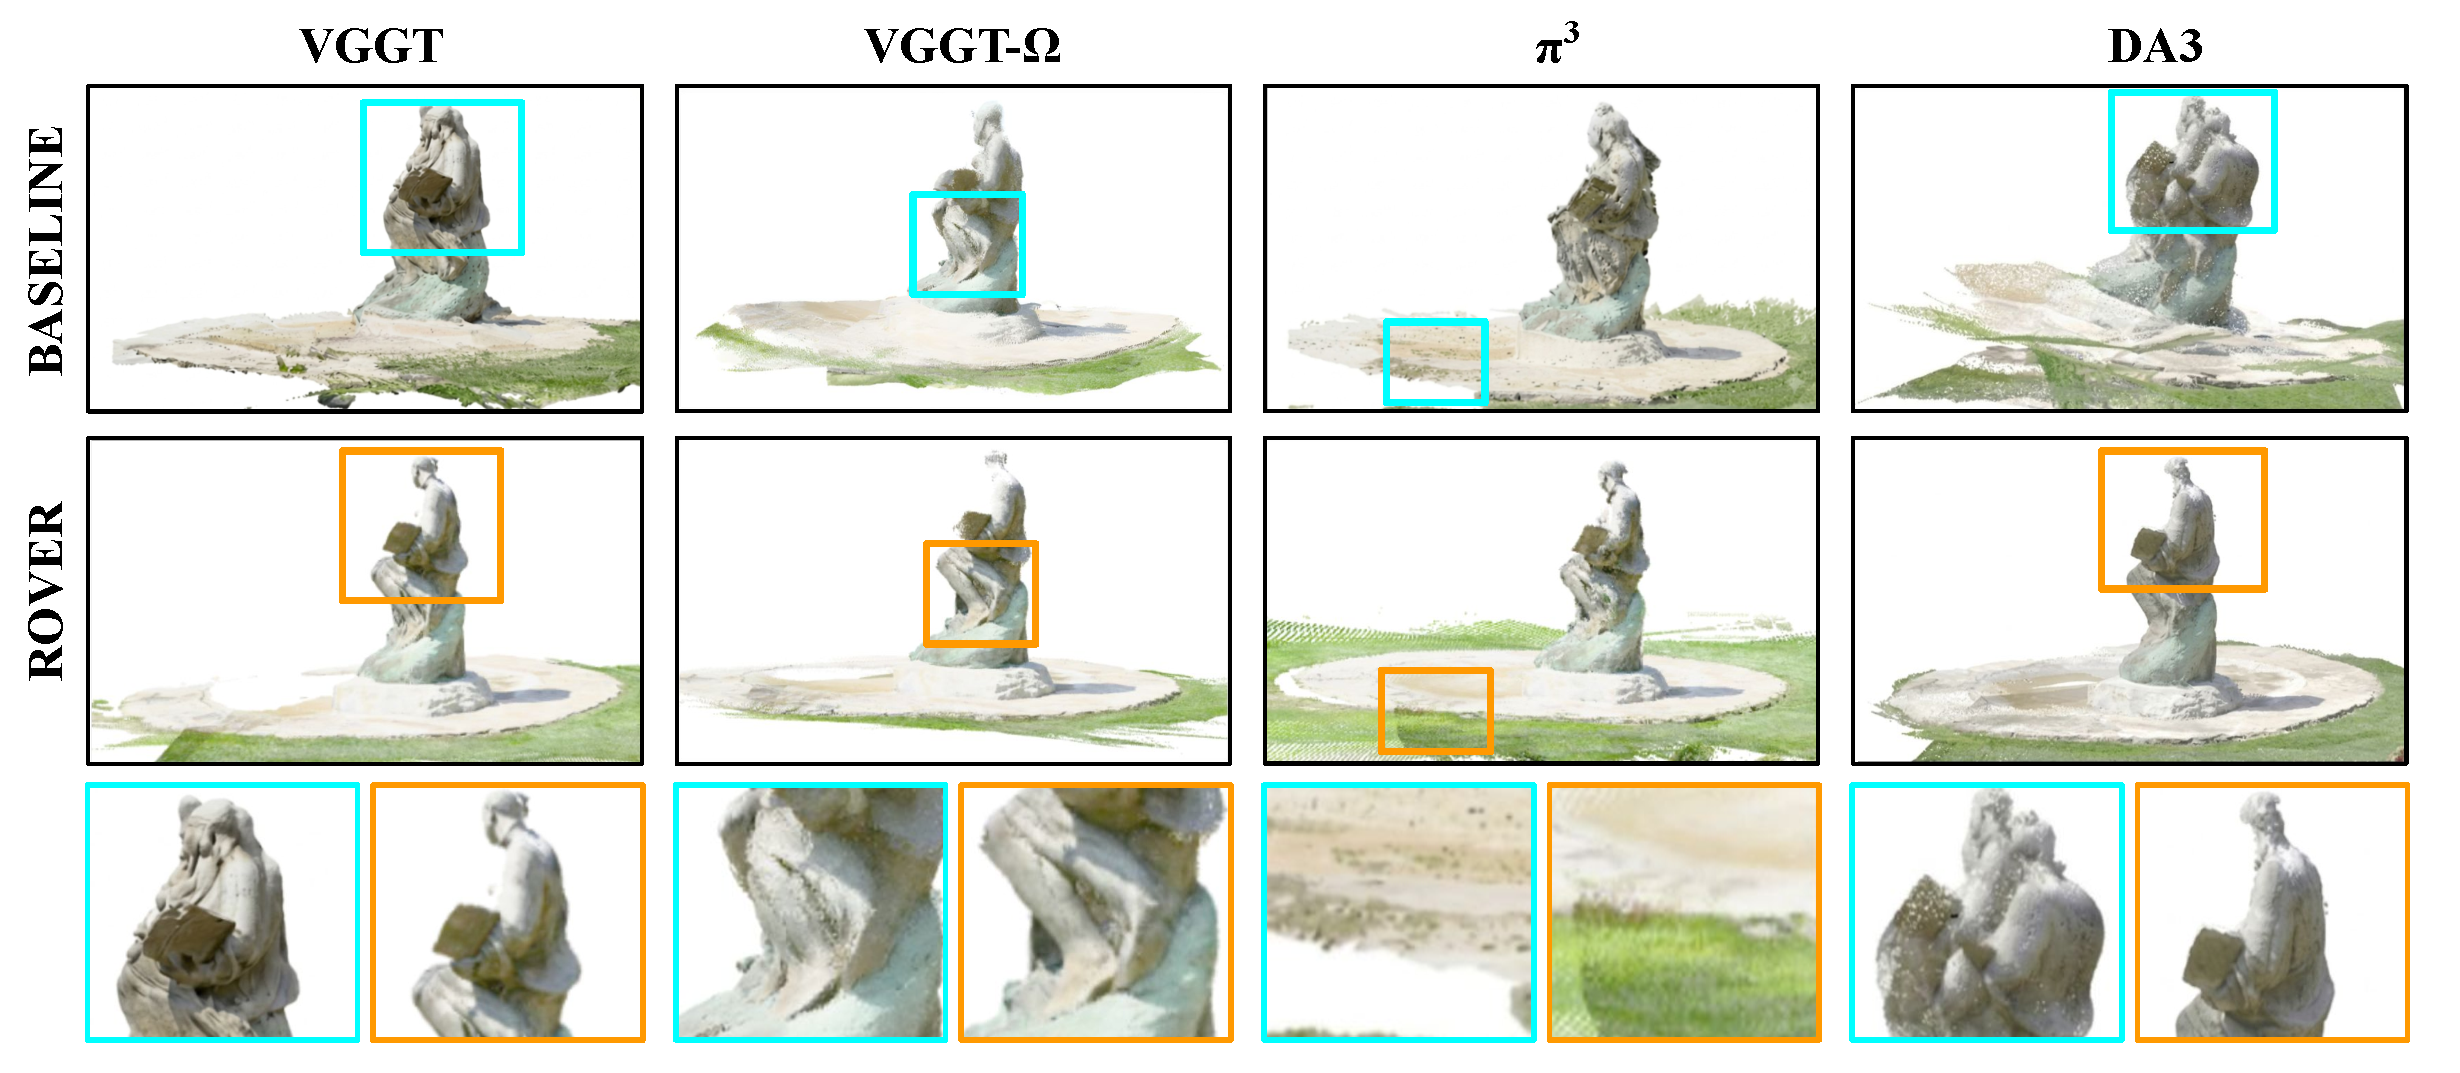
\includegraphics[width=\linewidth]{Figures/fig4/fig4.pdf}
    \caption{\textbf{Qualitative comparison.} Rotated input images to a feed-forward model produces a distorted point cloud (Baseline). Our method re-canonicalises the input images and then same model recovers geometrically faithful reconstruction. (ROVER)}
    \label{fig:our_result_tnt}
    \vspace{-4mm}
\end{figure*}

% % \begin{table*}[ht]
% \centering
% \caption{Point map estimation on 7-Scenes, NRGBD, and the Captured dataset (mean values $\pm$ std-dev).}
% \label{tab:pointmap_combined}
% \scriptsize
% \setlength{\tabcolsep}{3pt}
% \resizebox{\linewidth}{!}{\begin{tabular}{l cc cc cc cc cc cc cc cc cc}
% \toprule
% \multirow{3}{*}{Method} & \multicolumn{6}{c}{7-Scenes} & \multicolumn{6}{c}{NRGBD} & \multicolumn{6}{c}{Captured} \\
% \cmidrule(lr){2-7} \cmidrule(lr){8-13} \cmidrule(lr){14-19}
%  & \multicolumn{2}{c}{Acc. $\downarrow$} & \multicolumn{2}{c}{Comp. $\downarrow$} & \multicolumn{2}{c}{N.C. $\uparrow$}
%  & \multicolumn{2}{c}{Acc. $\downarrow$} & \multicolumn{2}{c}{Comp. $\downarrow$} & \multicolumn{2}{c}{N.C. $\uparrow$}
%  & \multicolumn{2}{c}{Acc. $\downarrow$} & \multicolumn{2}{c}{Comp. $\downarrow$} & \multicolumn{2}{c}{N.C. $\uparrow$} \\
% \cmidrule(lr){2-3} \cmidrule(lr){4-5} \cmidrule(lr){6-7} \cmidrule(lr){8-9} \cmidrule(lr){10-11} \cmidrule(lr){12-13} \cmidrule(lr){14-15} \cmidrule(lr){16-17} \cmidrule(lr){18-19}
%  & Ours & Baseline & Ours & Baseline & Ours & Baseline & Ours & Baseline & Ours & Baseline & Ours & Baseline & Ours & Baseline & Ours & Baseline & Ours & Baseline \\
% \midrule
% VGGT & \textbf{0.032 $\pm$ 0.012} & 0.063 $\pm$ 0.028 & \textbf{0.041 $\pm$ 0.013} & 0.128 $\pm$ 0.114 & \textbf{0.654 $\pm$ 0.011} & 0.614 $\pm$ 0.039 & \textbf{0.017 $\pm$ 0.002} & 0.049 $\pm$ 0.032 & \textbf{0.012 $\pm$ 0.001} & 0.091 $\pm$ 0.104 & \textbf{0.795 $\pm$ 0.009} & 0.721 $\pm$ 0.058 & \textbf{0.010 $\pm$ 0.004} & 0.022 $\pm$ 0.013 & \textbf{0.020 $\pm$ 0.016} & 0.039 $\pm$ 0.043 & \textbf{0.740 $\pm$ 0.051} & 0.677 $\pm$ 0.087 \\
% VGGT-$\Omega$ & \textbf{0.023 $\pm$ 0.004} & 0.028 $\pm$ 0.011 & \textbf{0.033 $\pm$ 0.006} & 0.033 $\pm$ 0.013 & \textbf{0.668 $\pm$ 0.007} & 0.667 $\pm$ 0.013 & \textbf{0.012 $\pm$ 0.009} & 0.016 $\pm$ 0.009 & \textbf{0.007 $\pm$ 0.005} & 0.008 $\pm$ 0.003 & \textbf{0.805 $\pm$ 0.019} & 0.786 $\pm$ 0.023 & \textbf{0.008 $\pm$ 0.003} & 0.009 $\pm$ 0.004 & \textbf{0.016 $\pm$ 0.010} & 0.017 $\pm$ 0.012 & \textbf{0.722 $\pm$ 0.044} & 0.712 $\pm$ 0.062 \\
% $\pi^3$ & \textbf{0.030 $\pm$ 0.012} & 0.066 $\pm$ 0.022 & \textbf{0.038 $\pm$ 0.017} & 0.129 $\pm$ 0.097 & \textbf{0.671 $\pm$ 0.015} & 0.625 $\pm$ 0.032 & \textbf{0.019 $\pm$ 0.010} & 0.046 $\pm$ 0.023 & \textbf{0.014 $\pm$ 0.007} & 0.089 $\pm$ 0.081 & \textbf{0.799 $\pm$ 0.015} & 0.734 $\pm$ 0.045 & \textbf{0.014 $\pm$ 0.005} & 0.035 $\pm$ 0.027 & \textbf{0.022 $\pm$ 0.013} & 0.049 $\pm$ 0.046 & \textbf{0.756 $\pm$ 0.048} & 0.697 $\pm$ 0.077 \\
% MapA & \textbf{0.078 $\pm$ 0.007} & 0.099 $\pm$ 0.020 & \textbf{0.116 $\pm$ 0.014} & 0.186 $\pm$ 0.082 & \textbf{0.627 $\pm$ 0.012} & 0.594 $\pm$ 0.027 & \textbf{0.083 $\pm$ 0.008} & 0.126 $\pm$ 0.033 & \textbf{0.068 $\pm$ 0.009} & 0.163 $\pm$ 0.125 & \textbf{0.730 $\pm$ 0.012} & 0.665 $\pm$ 0.056 & \textbf{0.463 $\pm$ 0.170} & 0.611 $\pm$ 0.253 & \textbf{0.945 $\pm$ 0.506} & 1.332 $\pm$ 0.885 & \textbf{0.752 $\pm$ 0.088} & 0.673 $\pm$ 0.106 \\
% DA3 & \textbf{0.037 $\pm$ 0.011} & 0.065 $\pm$ 0.027 & \textbf{0.047 $\pm$ 0.021} & 0.104 $\pm$ 0.078 & \textbf{0.667 $\pm$ 0.013} & 0.636 $\pm$ 0.031 & \textbf{0.016 $\pm$ 0.008} & 0.064 $\pm$ 0.041 & \textbf{0.011 $\pm$ 0.004} & 0.098 $\pm$ 0.149 & \textbf{0.807 $\pm$ 0.016} & 0.726 $\pm$ 0.072 & \textbf{0.251 $\pm$ 0.182} & 0.614 $\pm$ 0.311 & \textbf{0.338 $\pm$ 0.396} & 0.827 $\pm$ 0.813 & \textbf{0.762 $\pm$ 0.043} & 0.694 $\pm$ 0.082 \\
% \bottomrule
% \end{tabular}
% }
% \end{table*}

%%%%%%%%%%%%%%%%%%%%%%%%%%%%%%%%%%%%%%%%%%%%%%%%%%%%%%%%%

% \begin{table*}[ht]
% \centering
% \caption{Point map estimation on 7-Scenes, NRGBD, and the Captured dataset (mean values $\pm$ std-dev).}
% \label{tab:pointmap_combined}
% \scriptsize
% \setlength{\tabcolsep}{3pt}
% \resizebox{\linewidth}{!}{\begin{tabular}{l cc cc cc cc cc cc cc cc cc}
% \toprule
% \multirow{3}{*}{Method} & \multicolumn{6}{c}{7-Scenes} & \multicolumn{6}{c}{NRGBD} & \multicolumn{6}{c}{Captured} \\
% \cmidrule(lr){2-7} \cmidrule(lr){8-13} \cmidrule(lr){14-19}
%  & \multicolumn{2}{c}{Acc. $\downarrow$} & \multicolumn{2}{c}{Comp. $\downarrow$} & \multicolumn{2}{c}{N.C. $\uparrow$} & \multicolumn{2}{c}{Acc. $\downarrow$} & \multicolumn{2}{c}{Comp. $\downarrow$} & \multicolumn{2}{c}{N.C. $\uparrow$} & \multicolumn{2}{c}{Acc. $\downarrow$} & \multicolumn{2}{c}{Comp. $\downarrow$} & \multicolumn{2}{c}{N.C. $\uparrow$} \\
% \cmidrule(lr){2-3} \cmidrule(lr){4-5} \cmidrule(lr){6-7} \cmidrule(lr){8-9} \cmidrule(lr){10-11} \cmidrule(lr){12-13} \cmidrule(lr){14-15} \cmidrule(lr){16-17} \cmidrule(lr){18-19}
%  & Ours & Baseline & Ours & Baseline & Ours & Baseline & Ours & Baseline & Ours & Baseline & Ours & Baseline & Ours & Baseline & Ours & Baseline & Ours & Baseline \\
% \midrule
% VGGT & \textbf{0.03 $\pm$ 0.01} & 0.06 $\pm$ 0.03 & \textbf{0.04 $\pm$ 0.01} & 0.13 $\pm$ 0.11 & \textbf{0.65 $\pm$ 0.01} & 0.61 $\pm$ 0.04 & \textbf{0.02 $\pm$ 0.00} & 0.05 $\pm$ 0.03 & \textbf{0.01 $\pm$ 0.00} & 0.09 $\pm$ 0.10 & \textbf{0.79 $\pm$ 0.01} & 0.72 $\pm$ 0.06 & \textbf{0.01 $\pm$ 0.00} & 0.02 $\pm$ 0.01 & \textbf{0.02 $\pm$ 0.02} & 0.04 $\pm$ 0.04 & \textbf{0.74 $\pm$ 0.05} & 0.68 $\pm$ 0.09 \\
% VGGT-$\Omega$ & \textbf{0.02 $\pm$ 0.00} & 0.03 $\pm$ 0.01 & \textbf{0.03 $\pm$ 0.01} & 0.03 $\pm$ 0.01 & \textbf{0.67 $\pm$ 0.01} & 0.67 $\pm$ 0.01 & \textbf{0.01 $\pm$ 0.01} & 0.02 $\pm$ 0.01 & \textbf{0.01 $\pm$ 0.00} & 0.01 $\pm$ 0.00 & \textbf{0.81 $\pm$ 0.02} & 0.79 $\pm$ 0.02 & \textbf{0.01 $\pm$ 0.00} & 0.01 $\pm$ 0.00 & \textbf{0.02 $\pm$ 0.01} & 0.02 $\pm$ 0.01 & \textbf{0.72 $\pm$ 0.04} & 0.71 $\pm$ 0.06 \\
% $\pi^3$ & \textbf{0.03 $\pm$ 0.01} & 0.07 $\pm$ 0.02 & \textbf{0.04 $\pm$ 0.02} & 0.13 $\pm$ 0.10 & \textbf{0.67 $\pm$ 0.01} & 0.62 $\pm$ 0.03 & \textbf{0.02 $\pm$ 0.01} & 0.05 $\pm$ 0.02 & \textbf{0.01 $\pm$ 0.01} & 0.09 $\pm$ 0.08 & \textbf{0.80 $\pm$ 0.01} & 0.73 $\pm$ 0.04 & \textbf{0.01 $\pm$ 0.01} & 0.04 $\pm$ 0.03 & \textbf{0.02 $\pm$ 0.01} & 0.05 $\pm$ 0.05 & \textbf{0.76 $\pm$ 0.05} & 0.70 $\pm$ 0.08 \\
% MapAnything & \textbf{0.08 $\pm$ 0.01} & 0.10 $\pm$ 0.02 & \textbf{0.12 $\pm$ 0.01} & 0.19 $\pm$ 0.08 & \textbf{0.63 $\pm$ 0.01} & 0.59 $\pm$ 0.03 & \textbf{0.08 $\pm$ 0.01} & 0.13 $\pm$ 0.03 & \textbf{0.07 $\pm$ 0.01} & 0.16 $\pm$ 0.13 & \textbf{0.73 $\pm$ 0.01} & 0.67 $\pm$ 0.06 & \textbf{0.46 $\pm$ 0.17} & 0.61 $\pm$ 0.25 & \textbf{0.94 $\pm$ 0.51} & 1.33 $\pm$ 0.89 & \textbf{0.75 $\pm$ 0.09} & 0.67 $\pm$ 0.11 \\
% DepthAnything3 & \textbf{0.04 $\pm$ 0.01} & 0.07 $\pm$ 0.03 & \textbf{0.05 $\pm$ 0.02} & 0.10 $\pm$ 0.08 & \textbf{0.67 $\pm$ 0.01} & 0.64 $\pm$ 0.03 & \textbf{0.02 $\pm$ 0.01} & 0.06 $\pm$ 0.04 & \textbf{0.01 $\pm$ 0.00} & 0.10 $\pm$ 0.15 & \textbf{0.81 $\pm$ 0.02} & 0.73 $\pm$ 0.07 & \textbf{0.25 $\pm$ 0.18} & 0.61 $\pm$ 0.31 & \textbf{0.34 $\pm$ 0.40} & 0.83 $\pm$ 0.81 & \textbf{0.76 $\pm$ 0.04} & 0.69 $\pm$ 0.08 \\
% \bottomrule
% \end{tabular}
% }
% \end{table*}

%%%%%%%%%%%%%%%%%%%%%%%%%%%%%%%%%%%%%%%%%%%%%%%%%%%%%%%%%

% \usepackage{xcolor}
% \usepackage{colortbl}
% \definecolor{highlight}{gray}{0.92}

% \begin{table*}[ht]
% \centering
% \caption{Point map estimation on 7-Scenes, NRGBD, and Tanks \& Temples.}
% \label{tab:pointmap_combined}
% \small
% \renewcommand{\arraystretch}{1.25}
% \setlength{\tabcolsep}{3pt}

% \begin{tabular}{l ccc ccc ccc}
% \toprule
% & \multicolumn{3}{c}{\textbf{7-Scenes}} & \multicolumn{3}{c}{\textbf{NRGBD}} & \multicolumn{3}{c}{\textbf{Tanks \& Temples}} \\
% \cmidrule(lr){2-4} \cmidrule(lr){5-7} \cmidrule(lr){8-10}
% \textbf{Method} & Acc. $\downarrow$ & Comp. $\downarrow$ & N.C. $\uparrow$ & Acc. $\downarrow$ & Comp. $\downarrow$ & N.C. $\uparrow$ & Acc. $\downarrow$ & Comp. $\downarrow$ & N.C. $\uparrow$ \\
% \midrule

% VGGT & 0.06 {\tiny $\pm$ 0.03} & 0.13 {\tiny $\pm$ 0.11} & 0.61 {\tiny $\pm$ 0.04} & 0.05 {\tiny $\pm$ 0.03} & 0.09 {\tiny $\pm$ 0.10} & 0.72 {\tiny $\pm$ 0.06} & 0.08 {\tiny $\pm$ 0.03} & 0.14 {\tiny $\pm$ 0.08} & 0.60 {\tiny $\pm$ 0.04} \\
% \rowcolor{highlight}
% \hspace{0.5em}+ ROVER & \textbf{0.03} {\tiny $\pm$ 0.01} & \textbf{0.04} {\tiny $\pm$ 0.01} & \textbf{0.65} {\tiny $\pm$ 0.01} & \textbf{0.02} {\tiny $\pm$ 0.00} & \textbf{0.01} {\tiny $\pm$ 0.00} & \textbf{0.79} {\tiny $\pm$ 0.01} & \textbf{0.05} {\tiny $\pm$ 0.02} & \textbf{0.06} {\tiny $\pm$ 0.04} & \textbf{0.66} {\tiny $\pm$ 0.02} \\
% \addlinespace[3pt]

% VGGT-$\Omega$ & 0.03 {\tiny $\pm$ 0.01} & 0.03 {\tiny $\pm$ 0.01} & 0.67 {\tiny $\pm$ 0.01} & 0.02 {\tiny $\pm$ 0.01} & 0.01 {\tiny $\pm$ 0.00} & 0.79 {\tiny $\pm$ 0.02} & 0.06 {\tiny $\pm$ 0.02} & 0.08 {\tiny $\pm$ 0.05} & 0.64 {\tiny $\pm$ 0.02} \\
% \rowcolor{highlight}
% \hspace{0.5em}+ ROVER & \textbf{0.02} {\tiny $\pm$ 0.00} & \textbf{0.03} {\tiny $\pm$ 0.01} & \textbf{0.67} {\tiny $\pm$ 0.01} & \textbf{0.01} {\tiny $\pm$ 0.01} & \textbf{0.01} {\tiny $\pm$ 0.00} & \textbf{0.81} {\tiny $\pm$ 0.02} & \textbf{0.04} {\tiny $\pm$ 0.02} & \textbf{0.06} {\tiny $\pm$ 0.04} & \textbf{0.68} {\tiny $\pm$ 0.02} \\

% \bottomrule
% \end{tabular}
% \end{table*}


\begin{table*}[ht]
\centering
\caption{Point map estimation on 7-Scenes, NRGBD, and Tanks \& Temples.}
\label{tab:pointmap_combined}
\small
\renewcommand{\arraystretch}{1}
\setlength{\tabcolsep}{3pt}

\resizebox{\linewidth}{!}{
\begin{tabular}{l ccc ccc ccc}
\toprule
& \multicolumn{3}{c}{\textbf{7-Scenes}} & \multicolumn{3}{c}{\textbf{NRGBD}} & \multicolumn{3}{c}{\textbf{Tanks \& Temples}} \\
\cmidrule(lr){2-4} \cmidrule(lr){5-7} \cmidrule(lr){8-10}
\textbf{Method} & Acc. $\downarrow$ & Comp. $\downarrow$ & N.C. $\uparrow$ & Acc. $\downarrow$ & Comp. $\downarrow$ & N.C. $\uparrow$ & Acc. $\downarrow$ & Comp. $\downarrow$ & N.C. $\uparrow$ \\
\midrule

VGGT & 0.06 {\tiny $\pm$ 0.03} & 0.13 {\tiny $\pm$ 0.11} & 0.61 {\tiny $\pm$ 0.04} & 0.05 {\tiny $\pm$ 0.03} & 0.09 {\tiny $\pm$ 0.10} & 0.72 {\tiny $\pm$ 0.06} & 0.08 {\tiny $\pm$ 0.03} & 0.14 {\tiny $\pm$ 0.08} & 0.60 {\tiny $\pm$ 0.04} \\
\rowcolor{highlight}
\quad + ROVER & \textbf{0.03 {\tiny $\pm$ 0.01}} & \textbf{0.04 {\tiny $\pm$ 0.01}} & \textbf{0.65 {\tiny $\pm$ 0.01}} & \textbf{0.02 {\tiny $\pm$ 0.00}} & \textbf{0.01 {\tiny $\pm$ 0.00}} & \textbf{0.79 {\tiny $\pm$ 0.01}} & \textbf{0.05 {\tiny $\pm$ 0.02}} & \textbf{0.06 {\tiny $\pm$ 0.04}} & \textbf{0.66 {\tiny $\pm$ 0.02}} \\
\addlinespace[3pt]

VGGT-$\Omega$ & 0.03 {\tiny $\pm$ 0.01} & 0.03 {\tiny $\pm$ 0.01} & 0.67 {\tiny $\pm$ 0.01} & 0.02 {\tiny $\pm$ 0.01} & 0.01 {\tiny $\pm$ 0.00} & 0.79 {\tiny $\pm$ 0.02} & 0.06 {\tiny $\pm$ 0.02} & 0.08 {\tiny $\pm$ 0.05} & 0.64 {\tiny $\pm$ 0.02} \\
\rowcolor{highlight}
\quad + ROVER & \textbf{0.02 {\tiny $\pm$ 0.00}} & \textbf{0.03 {\tiny $\pm$ 0.01}} & \textbf{0.67 {\tiny $\pm$ 0.01}} & \textbf{0.01 {\tiny $\pm$ 0.01}} & \textbf{0.01 {\tiny $\pm$ 0.00}} & \textbf{0.81 {\tiny $\pm$ 0.02}} & \textbf{0.04 {\tiny $\pm$ 0.02}} & \textbf{0.06 {\tiny $\pm$ 0.04}} & \textbf{0.68 {\tiny $\pm$ 0.02}} \\
\addlinespace[3pt]

$\pi^3$ & 0.07 {\tiny $\pm$ 0.02} & 0.13 {\tiny $\pm$ 0.10} & 0.62 {\tiny $\pm$ 0.03} & 0.05 {\tiny $\pm$ 0.02} & 0.09 {\tiny $\pm$ 0.08} & 0.73 {\tiny $\pm$ 0.04} & 0.09 {\tiny $\pm$ 0.03} & 0.15 {\tiny $\pm$ 0.09} & 0.59 {\tiny $\pm$ 0.03} \\
\rowcolor{highlight}
\quad + ROVER & \textbf{0.03 {\tiny $\pm$ 0.01}} & \textbf{0.04 {\tiny $\pm$ 0.02}} & \textbf{0.67 {\tiny $\pm$ 0.01}} & \textbf{0.02 {\tiny $\pm$ 0.01}} & \textbf{0.01 {\tiny $\pm$ 0.01}} & \textbf{0.80 {\tiny $\pm$ 0.01}} & \textbf{0.05 {\tiny $\pm$ 0.02}} & \textbf{0.07 {\tiny $\pm$ 0.04}} & \textbf{0.65 {\tiny $\pm$ 0.02}} \\

\bottomrule
\end{tabular}
}
\end{table*}
% \begin{table*}[ht]
% \centering
% \caption{Point map estimation on 7-Scenes, NRGBD, and the ETH3D with ROVER. Results are averaged across the full rotation-fraction sweep per scene. Results are averaged over all $m$}
% \label{tab:pointmap_combined}
% \small
% \renewcommand{\arraystretch}{1.2}
% \setlength{\tabcolsep}{2pt}

% \resizebox{\linewidth}{!}{
% \begin{tabular}{l *{3}{cc} *{3}{cc} *{3}{cc}}
% \toprule
% & \multicolumn{6}{c}{\textbf{7-Scenes}} & \multicolumn{6}{c}{\textbf{NRGBD}} & \multicolumn{6}{c}{\textbf{ETH3D}} \\
% \cmidrule(lr){2-7} \cmidrule(lr){8-13} \cmidrule(lr){14-19}
% & \multicolumn{2}{c}{Acc. $\downarrow$} & \multicolumn{2}{c}{Comp. $\downarrow$} & \multicolumn{2}{c}{N.C. $\uparrow$}
% & \multicolumn{2}{c}{Acc. $\downarrow$} & \multicolumn{2}{c}{Comp. $\downarrow$} & \multicolumn{2}{c}{N.C. $\uparrow$}
% & \multicolumn{2}{c}{Acc. $\downarrow$} & \multicolumn{2}{c}{Comp. $\downarrow$} & \multicolumn{2}{c}{N.C. $\uparrow$} \\
% \cmidrule(lr){2-3} \cmidrule(lr){4-5} \cmidrule(lr){6-7} \cmidrule(lr){8-9} \cmidrule(lr){10-11} \cmidrule(lr){12-13} \cmidrule(lr){14-15} \cmidrule(lr){16-17} \cmidrule(lr){18-19}
% \textbf{Method} & Base & Ours & Base & Ours & Base & Ours & Base & Ours & Base & Ours & Base & Ours & Base & Ours & Base & Ours & Base & Ours \\
% \midrule

% VGGT 
% & \makecell{0.06 \\ {\tiny $\pm$ 0.03}} & \makecell{\textbf{0.03} \\ {\tiny $\pm$ 0.01}} 
% & \makecell{0.13 \\ {\tiny $\pm$ 0.11}} & \makecell{\textbf{0.04} \\ {\tiny $\pm$ 0.01}} 
% & \makecell{0.61 \\ {\tiny $\pm$ 0.04}} & \makecell{\textbf{0.65} \\ {\tiny $\pm$ 0.01}} 
% & \makecell{0.05 \\ {\tiny $\pm$ 0.03}} & \makecell{\textbf{0.02} \\ {\tiny $\pm$ 0.00}} 
% & \makecell{0.09 \\ {\tiny $\pm$ 0.10}} & \makecell{\textbf{0.01} \\ {\tiny $\pm$ 0.00}} 
% & \makecell{0.72 \\ {\tiny $\pm$ 0.06}} & \makecell{\textbf{0.79} \\ {\tiny $\pm$ 0.01}} 
% & \makecell{0.20 \\ {\tiny $\pm$ 0.07}} & \makecell{\textbf{0.18} \\ {\tiny $\pm$ 0.06}} 
% & \makecell{0.11 \\ {\tiny $\pm$ 0.04}} & \makecell{\textbf{0.08} \\ {\tiny $\pm$ 0.02}} 
% & \makecell{0.77 \\ {\tiny $\pm$ 0.04}} & \makecell{\textbf{0.79} \\ {\tiny $\pm$ 0.03}} \\
% \addlinespace[3pt]

% VGGT-$\Omega$ 
% & \makecell{0.03 \\ {\tiny $\pm$ 0.01}} & \makecell{\textbf{0.02} \\ {\tiny $\pm$ 0.00}} 
% & \makecell{0.03 \\ {\tiny $\pm$ 0.01}} & \makecell{\textbf{0.03} \\ {\tiny $\pm$ 0.01}} 
% & \makecell{0.67 \\ {\tiny $\pm$ 0.01}} & \makecell{\textbf{0.67} \\ {\tiny $\pm$ 0.01}} 
% & \makecell{0.02 \\ {\tiny $\pm$ 0.01}} & \makecell{\textbf{0.01} \\ {\tiny $\pm$ 0.01}} 
% & \makecell{\textbf{0.01} \\ {\tiny $\pm$ 0.00}} & \makecell{\textbf{0.01} \\ {\tiny $\pm$ 0.00}} 
% & \makecell{0.79 \\ {\tiny $\pm$ 0.02}} & \makecell{\textbf{0.81} \\ {\tiny $\pm$ 0.02}} 
% & \makecell{0.07 \\ {\tiny $\pm$ 0.03}} & \makecell{\textbf{0.06} \\ {\tiny $\pm$ 0.02}} 
% & \makecell{\textbf{0.05} \\ {\tiny $\pm$ 0.02}} & \makecell{\textbf{0.05} \\ {\tiny $\pm$ 0.02}} 
% & \makecell{\textbf{0.85} \\ {\tiny $\pm$ 0.03}} & \makecell{\textbf{0.85} \\ {\tiny $\pm$ 0.03}} \\
% \addlinespace[3pt]

% $\pi^3$ 
% & \makecell{0.07 \\ {\tiny $\pm$ 0.02}} & \makecell{\textbf{0.03} \\ {\tiny $\pm$ 0.01}} 
% & \makecell{0.13 \\ {\tiny $\pm$ 0.10}} & \makecell{\textbf{0.04} \\ {\tiny $\pm$ 0.02}} 
% & \makecell{0.62 \\ {\tiny $\pm$ 0.03}} & \makecell{\textbf{0.67} \\ {\tiny $\pm$ 0.01}} 
% & \makecell{0.05 \\ {\tiny $\pm$ 0.02}} & \makecell{\textbf{0.02} \\ {\tiny $\pm$ 0.01}} 
% & \makecell{0.09 \\ {\tiny $\pm$ 0.08}} & \makecell{\textbf{0.01} \\ {\tiny $\pm$ 0.01}} 
% & \makecell{0.73 \\ {\tiny $\pm$ 0.04}} & \makecell{\textbf{0.80} \\ {\tiny $\pm$ 0.01}} 
% & \makecell{0.09 \\ {\tiny $\pm$ 0.03}} & \makecell{\textbf{0.08} \\ {\tiny $\pm$ 0.02}} 
% & \makecell{0.07 \\ {\tiny $\pm$ 0.02}} & \makecell{\textbf{0.06} \\ {\tiny $\pm$ 0.02}} 
% & \makecell{0.84 \\ {\tiny $\pm$ 0.02}} & \makecell{\textbf{0.85} \\ {\tiny $\pm$ 0.02}} \\
% \addlinespace[3pt]

% MapA.
% & \makecell{0.10 \\ {\tiny $\pm$ 0.02}} & \makecell{\textbf{0.08} \\ {\tiny $\pm$ 0.01}} 
% & \makecell{0.19 \\ {\tiny $\pm$ 0.08}} & \makecell{\textbf{0.12} \\ {\tiny $\pm$ 0.01}} 
% & \makecell{0.59 \\ {\tiny $\pm$ 0.03}} & \makecell{\textbf{0.63} \\ {\tiny $\pm$ 0.01}} 
% & \makecell{0.13 \\ {\tiny $\pm$ 0.03}} & \makecell{\textbf{0.08} \\ {\tiny $\pm$ 0.01}} 
% & \makecell{0.16 \\ {\tiny $\pm$ 0.13}} & \makecell{\textbf{0.07} \\ {\tiny $\pm$ 0.01}} 
% & \makecell{0.67 \\ {\tiny $\pm$ 0.06}} & \makecell{\textbf{0.73} \\ {\tiny $\pm$ 0.01}} 
% & \makecell{0.16 \\ {\tiny $\pm$ 0.03}} & \makecell{\textbf{0.15} \\ {\tiny $\pm$ 0.03}} 
% & \makecell{0.39 \\ {\tiny $\pm$ 0.36}} & \makecell{\textbf{0.36} \\ {\tiny $\pm$ 0.29}} 
% & \makecell{0.75 \\ {\tiny $\pm$ 0.03}} & \makecell{\textbf{0.76} \\ {\tiny $\pm$ 0.02}} \\
% \addlinespace[3pt]

% DA3
% & \makecell{0.07 \\ {\tiny $\pm$ 0.03}} & \makecell{\textbf{0.04} \\ {\tiny $\pm$ 0.01}} 
% & \makecell{0.10 \\ {\tiny $\pm$ 0.08}} & \makecell{\textbf{0.05} \\ {\tiny $\pm$ 0.02}} 
% & \makecell{0.64 \\ {\tiny $\pm$ 0.03}} & \makecell{\textbf{0.67} \\ {\tiny $\pm$ 0.01}} 
% & \makecell{0.06 \\ {\tiny $\pm$ 0.04}} & \makecell{\textbf{0.02} \\ {\tiny $\pm$ 0.01}} 
% & \makecell{0.10 \\ {\tiny $\pm$ 0.15}} & \makecell{\textbf{0.01} \\ {\tiny $\pm$ 0.00}} 
% & \makecell{0.73 \\ {\tiny $\pm$ 0.07}} & \makecell{\textbf{0.81} \\ {\tiny $\pm$ 0.02}} 
% & \makecell{\textbf{0.11} \\ {\tiny $\pm$ 0.02}} & \makecell{\textbf{0.11} \\ {\tiny $\pm$ 0.00}} 
% & \makecell{0.12 \\ {\tiny $\pm$ 0.01}} & \makecell{\textbf{0.10} \\ {\tiny $\pm$ 0.01}} 
% & \makecell{\textbf{0.82} \\ {\tiny $\pm$ 0.01}} & \makecell{\textbf{0.82} \\ {\tiny $\pm$ 0.01}} \\

% \bottomrule
% \end{tabular}


% }
% \vspace{-2mm}
% \end{table*}

\begin{table*}[ht]
\centering
\caption{\textbf{Point map estimation} on 7-Scenes, NRGB-D, and RotMV with ROVER. Results are averaged across the full rotation-fraction sweep per scene.}
\label{tab:pointmap_combined}
\small
\renewcommand{\arraystretch}{1.2}
\setlength{\tabcolsep}{2pt}

\resizebox{\linewidth}{!}{
\begin{tabular}{l *{3}{cc} *{3}{cc} *{3}{cc}}
\toprule
& \multicolumn{6}{c}{\textbf{7-Scenes}} & \multicolumn{6}{c}{\textbf{NRGB-D}} & \multicolumn{6}{c}{\textbf{RotMV}} \\
\cmidrule(lr){2-7} \cmidrule(lr){8-13} \cmidrule(lr){14-19}
& \multicolumn{2}{c}{Acc. $\downarrow$} & \multicolumn{2}{c}{Comp. $\downarrow$} & \multicolumn{2}{c}{N.C. $\uparrow$}
& \multicolumn{2}{c}{Acc. $\downarrow$} & \multicolumn{2}{c}{Comp. $\downarrow$} & \multicolumn{2}{c}{N.C. $\uparrow$}
& \multicolumn{2}{c}{Acc. $\downarrow$} & \multicolumn{2}{c}{Comp. $\downarrow$} & \multicolumn{2}{c}{N.C. $\uparrow$} \\
\cmidrule(lr){2-3} \cmidrule(lr){4-5} \cmidrule(lr){6-7} \cmidrule(lr){8-9} \cmidrule(lr){10-11} \cmidrule(lr){12-13} \cmidrule(lr){14-15} \cmidrule(lr){16-17} \cmidrule(lr){18-19}
\textbf{Method} & Base & Ours & Base & Ours & Base & Ours & Base & Ours & Base & Ours & Base & Ours & Base & Ours & Base & Ours & Base & Ours \\
\midrule

VGGT 
& \makecell{0.06 \\ {\tiny $\pm$ 0.03}} & \makecell{\textbf{0.03} \\ {\tiny $\pm$ 0.01}} 
& \makecell{0.13 \\ {\tiny $\pm$ 0.11}} & \makecell{\textbf{0.04} \\ {\tiny $\pm$ 0.01}} 
& \makecell{0.61 \\ {\tiny $\pm$ 0.04}} & \makecell{\textbf{0.65} \\ {\tiny $\pm$ 0.01}} 
& \makecell{0.05 \\ {\tiny $\pm$ 0.03}} & \makecell{\textbf{0.02} \\ {\tiny $\pm$ 0.00}} 
& \makecell{0.09 \\ {\tiny $\pm$ 0.10}} & \makecell{\textbf{0.01} \\ {\tiny $\pm$ 0.00}} 
& \makecell{0.72 \\ {\tiny $\pm$ 0.06}} & \makecell{\textbf{0.79} \\ {\tiny $\pm$ 0.01}} 
& \makecell{0.02 \\ {\tiny $\pm$ 0.01}} & \makecell{\textbf{0.01} \\ {\tiny $\pm$ 0.00}} 
& \makecell{0.04 \\ {\tiny $\pm$ 0.04}} & \makecell{\textbf{0.02} \\ {\tiny $\pm$ 0.02}} 
& \makecell{0.68 \\ {\tiny $\pm$ 0.09}} & \makecell{\textbf{0.74} \\ {\tiny $\pm$ 0.05}} \\
\addlinespace[3pt]

VGGT-$\Omega$ 
& \makecell{0.03 \\ {\tiny $\pm$ 0.01}} & \makecell{\textbf{0.02} \\ {\tiny $\pm$ 0.00}} 
& \makecell{0.03 \\ {\tiny $\pm$ 0.01}} & \makecell{\textbf{0.03} \\ {\tiny $\pm$ 0.01}} 
& \makecell{0.67 \\ {\tiny $\pm$ 0.01}} & \makecell{\textbf{0.67} \\ {\tiny $\pm$ 0.01}} 
& \makecell{0.02 \\ {\tiny $\pm$ 0.01}} & \makecell{\textbf{0.01} \\ {\tiny $\pm$ 0.01}} 
& \makecell{\textbf{0.01} \\ {\tiny $\pm$ 0.00}} & \makecell{\textbf{0.01} \\ {\tiny $\pm$ 0.00}} 
& \makecell{0.79 \\ {\tiny $\pm$ 0.02}} & \makecell{\textbf{0.81} \\ {\tiny $\pm$ 0.02}} 
& \makecell{\textbf{0.01} \\ {\tiny $\pm$ 0.00}} & \makecell{\textbf{0.01} \\ {\tiny $\pm$ 0.00}} 
& \makecell{\textbf{0.02} \\ {\tiny $\pm$ 0.01}} & \makecell{\textbf{0.02} \\ {\tiny $\pm$ 0.01}} 
& \makecell{0.71 \\ {\tiny $\pm$ 0.06}} & \makecell{\textbf{0.72} \\ {\tiny $\pm$ 0.04}} \\
\addlinespace[3pt]

$\pi^3$ 
& \makecell{0.07 \\ {\tiny $\pm$ 0.02}} & \makecell{\textbf{0.03} \\ {\tiny $\pm$ 0.01}} 
& \makecell{0.13 \\ {\tiny $\pm$ 0.10}} & \makecell{\textbf{0.04} \\ {\tiny $\pm$ 0.02}} 
& \makecell{0.62 \\ {\tiny $\pm$ 0.03}} & \makecell{\textbf{0.67} \\ {\tiny $\pm$ 0.01}} 
& \makecell{0.05 \\ {\tiny $\pm$ 0.02}} & \makecell{\textbf{0.02} \\ {\tiny $\pm$ 0.01}} 
& \makecell{0.09 \\ {\tiny $\pm$ 0.08}} & \makecell{\textbf{0.01} \\ {\tiny $\pm$ 0.01}} 
& \makecell{0.73 \\ {\tiny $\pm$ 0.04}} & \makecell{\textbf{0.80} \\ {\tiny $\pm$ 0.01}} 
& \makecell{0.04 \\ {\tiny $\pm$ 0.03}} & \makecell{\textbf{0.01} \\ {\tiny $\pm$ 0.01}} 
& \makecell{0.05 \\ {\tiny $\pm$ 0.05}} & \makecell{\textbf{0.02} \\ {\tiny $\pm$ 0.01}} 
& \makecell{0.70 \\ {\tiny $\pm$ 0.08}} & \makecell{\textbf{0.76} \\ {\tiny $\pm$ 0.05}} \\
\addlinespace[3pt]

MapA.
& \makecell{0.10 \\ {\tiny $\pm$ 0.02}} & \makecell{\textbf{0.08} \\ {\tiny $\pm$ 0.01}} 
& \makecell{0.19 \\ {\tiny $\pm$ 0.08}} & \makecell{\textbf{0.12} \\ {\tiny $\pm$ 0.01}} 
& \makecell{0.59 \\ {\tiny $\pm$ 0.03}} & \makecell{\textbf{0.63} \\ {\tiny $\pm$ 0.01}} 
& \makecell{0.13 \\ {\tiny $\pm$ 0.03}} & \makecell{\textbf{0.08} \\ {\tiny $\pm$ 0.01}} 
& \makecell{0.16 \\ {\tiny $\pm$ 0.13}} & \makecell{\textbf{0.07} \\ {\tiny $\pm$ 0.01}} 
& \makecell{0.67 \\ {\tiny $\pm$ 0.06}} & \makecell{\textbf{0.73} \\ {\tiny $\pm$ 0.01}} 
& \makecell{0.61 \\ {\tiny $\pm$ 0.25}} & \makecell{\textbf{0.46} \\ {\tiny $\pm$ 0.17}} 
& \makecell{1.33 \\ {\tiny $\pm$ 0.89}} & \makecell{\textbf{0.95} \\ {\tiny $\pm$ 0.51}} 
& \makecell{0.67 \\ {\tiny $\pm$ 0.11}} & \makecell{\textbf{0.75} \\ {\tiny $\pm$ 0.09}} \\
\addlinespace[3pt]

DA3
& \makecell{0.07 \\ {\tiny $\pm$ 0.03}} & \makecell{\textbf{0.04} \\ {\tiny $\pm$ 0.01}} 
& \makecell{0.10 \\ {\tiny $\pm$ 0.08}} & \makecell{\textbf{0.05} \\ {\tiny $\pm$ 0.02}} 
& \makecell{0.64 \\ {\tiny $\pm$ 0.03}} & \makecell{\textbf{0.67} \\ {\tiny $\pm$ 0.01}} 
& \makecell{0.06 \\ {\tiny $\pm$ 0.04}} & \makecell{\textbf{0.02} \\ {\tiny $\pm$ 0.01}} 
& \makecell{0.10 \\ {\tiny $\pm$ 0.15}} & \makecell{\textbf{0.01} \\ {\tiny $\pm$ 0.00}} 
& \makecell{0.73 \\ {\tiny $\pm$ 0.07}} & \makecell{\textbf{0.81} \\ {\tiny $\pm$ 0.02}} 
& \makecell{0.61 \\ {\tiny $\pm$ 0.31}} & \makecell{\textbf{0.25} \\ {\tiny $\pm$ 0.18}} 
& \makecell{0.83 \\ {\tiny $\pm$ 0.81}} & \makecell{\textbf{0.34} \\ {\tiny $\pm$ 0.40}} 
& \makecell{0.69 \\ {\tiny $\pm$ 0.08}} & \makecell{\textbf{0.76} \\ {\tiny $\pm$ 0.04}} \\

\bottomrule
\end{tabular}


}
\vspace{-2mm}
\end{table*}

Table~\ref{tab:pointmap_combined} shows that ROVER consistently improves point-map estimation across all models and datasets.
On 7-Scenes, our method provides gains across all models: Comp. errors drop by up to $3\times$ (VGGT: $0.13$ to $0.04$; $\pi^3$: $0.13$ to $0.04$), and N.C. improves consistently, with the largest gain for $\pi^3$ ($0.62$ to $0.67$). Variance is also reduced, indicating more stable predictions by ROVER. On NRGB-D, VGGT-$\Omega$ and DA3 achieve N.C. gains of $0.02$ and $0.08$ respectively, while Comp. errors fall for several models (e.g., VGGT: $0.09$ to $0.01$). On RotMV, ROVER improves point-map quality across all models: N.C.\ gains are observed for VGGT-$\Omega$ ($0.71$ to $0.72$), VGGT ($0.68$ to $0.74$), and DA3 ($0.69$ to $0.76$), while Accuracy improves for $\pi^3$ ($0.04$ to $0.01$) and 
MapA. ($0.61$ to $0.46$).
 
% % \begin{table*}[ht]
% \centering
% \caption{Camera pose estimation on 7-Scenes, NRGBD, and the Captured dataset (mean values $\pm$ std-dev).}
% \label{tab:pose_combined}
% \scriptsize
% \setlength{\tabcolsep}{3pt}
% \resizebox{\linewidth}{!}{\begin{tabular}{l cc cc cc cc cc cc cc cc cc}
% \toprule
% \multirow{3}{*}{Method} & \multicolumn{6}{c}{7-Scenes} & \multicolumn{6}{c}{NRGBD} & \multicolumn{6}{c}{Captured} \\
% \cmidrule(lr){2-7} \cmidrule(lr){8-13} \cmidrule(lr){14-19}
%  & \multicolumn{2}{c}{RAcc$_{30}$ $\uparrow$} & \multicolumn{2}{c}{TAcc$_{30}$ $\uparrow$} & \multicolumn{2}{c}{AUC$_{30}$ $\uparrow$} & \multicolumn{2}{c}{RAcc$_{30}$ $\uparrow$} & \multicolumn{2}{c}{TAcc$_{30}$ $\uparrow$} & \multicolumn{2}{c}{AUC$_{30}$ $\uparrow$} & \multicolumn{2}{c}{RAcc$_{30}$ $\uparrow$} & \multicolumn{2}{c}{TAcc$_{30}$ $\uparrow$} & \multicolumn{2}{c}{AUC$_{30}$ $\uparrow$} \\
% \cmidrule(lr){2-3} \cmidrule(lr){4-5} \cmidrule(lr){6-7} \cmidrule(lr){8-9} \cmidrule(lr){10-11} \cmidrule(lr){12-13} \cmidrule(lr){14-15} \cmidrule(lr){16-17} \cmidrule(lr){18-19}
%  & Ours & Baseline & Ours & Baseline & Ours & Baseline & Ours & Baseline & Ours & Baseline & Ours & Baseline & Ours & Baseline & Ours & Baseline & Ours & Baseline \\
% \midrule
% VGGT & \textbf{98.630 $\pm$ 2.376} & 77.488 $\pm$ 19.176 & \textbf{94.501 $\pm$ 5.762} & 74.916 $\pm$ 17.259 & \textbf{78.508 $\pm$ 6.636} & 53.970 $\pm$ 20.867 & \textbf{100.000 $\pm$ 0.000} & 90.495 $\pm$ 12.946 & \textbf{99.887 $\pm$ 0.159} & 90.901 $\pm$ 10.154 & \textbf{97.132 $\pm$ 0.953} & 78.216 $\pm$ 17.154 & \textbf{96.850 $\pm$ 3.306} & 88.461 $\pm$ 15.139 & \textbf{97.994 $\pm$ 2.304} & 90.944 $\pm$ 12.585 & \textbf{84.147 $\pm$ 8.342} & 72.173 $\pm$ 19.150 \\
% VGGT-$\Omega$ & \textbf{99.913 $\pm$ 0.389} & 99.204 $\pm$ 2.584 & \textbf{98.269 $\pm$ 1.237} & 96.170 $\pm$ 4.342 & \textbf{83.628 $\pm$ 3.186} & 78.127 $\pm$ 7.774 & \textbf{100.000 $\pm$ 0.000} & \textbf{100.000 $\pm$ 0.000} & \textbf{99.964 $\pm$ 0.050} & 99.388 $\pm$ 0.761 & \textbf{98.023 $\pm$ 0.905} & 93.006 $\pm$ 3.945 & \textbf{98.862 $\pm$ 1.595} & 98.679 $\pm$ 2.189 & \textbf{99.832 $\pm$ 0.232} & 99.573 $\pm$ 0.788 & \textbf{85.597 $\pm$ 6.619} & 83.572 $\pm$ 7.659 \\
% $\pi^3$ & \textbf{98.066 $\pm$ 3.004} & 78.600 $\pm$ 13.680 & \textbf{96.748 $\pm$ 3.067} & 76.681 $\pm$ 14.052 & \textbf{80.712 $\pm$ 5.414} & 57.050 $\pm$ 15.497 & \textbf{99.898 $\pm$ 0.366} & 91.276 $\pm$ 9.308 & \textbf{99.817 $\pm$ 0.443} & 90.490 $\pm$ 7.706 & \textbf{95.212 $\pm$ 1.344} & 79.091 $\pm$ 10.716 & \textbf{98.943 $\pm$ 1.481} & 92.915 $\pm$ 10.416 & \textbf{99.817 $\pm$ 0.293} & 93.946 $\pm$ 8.614 & \textbf{85.252 $\pm$ 6.599} & 74.622 $\pm$ 13.220 \\
% MapA & \textbf{98.095 $\pm$ 2.670} & 74.286 $\pm$ 16.485 & \textbf{86.998 $\pm$ 5.975} & 63.906 $\pm$ 14.728 & \textbf{62.773 $\pm$ 7.719} & 36.844 $\pm$ 16.901 & \textbf{99.898 $\pm$ 0.651} & 75.811 $\pm$ 21.306 & \textbf{98.494 $\pm$ 1.199} & 71.123 $\pm$ 19.261 & \textbf{87.221 $\pm$ 3.777} & 46.798 $\pm$ 22.840 & \textbf{98.426 $\pm$ 2.300} & 68.551 $\pm$ 24.052 & \textbf{97.999 $\pm$ 1.640} & 73.569 $\pm$ 18.964 & \textbf{80.733 $\pm$ 7.921} & 44.558 $\pm$ 25.058 \\
% DA3 & \textbf{98.220 $\pm$ 2.682} & 82.471 $\pm$ 14.365 & \textbf{93.438 $\pm$ 5.671} & 79.138 $\pm$ 12.353 & \textbf{80.515 $\pm$ 5.989} & 58.667 $\pm$ 16.122 & \textbf{99.864 $\pm$ 0.417} & 89.510 $\pm$ 14.871 & \textbf{99.794 $\pm$ 0.597} & 88.561 $\pm$ 12.506 & \textbf{98.509 $\pm$ 1.615} & 73.373 $\pm$ 18.485 & \textbf{97.314 $\pm$ 4.809} & 80.479 $\pm$ 20.777 & \textbf{97.938 $\pm$ 3.533} & 85.232 $\pm$ 15.352 & \textbf{82.930 $\pm$ 9.692} & 60.886 $\pm$ 22.568 \\
% \bottomrule
% \end{tabular}
% }
% \end{table*}

% \begin{table*}[ht]
% \centering
% \caption{Camera pose estimation on 7-Scenes, NRGBD, and the Captured dataset (mean values $\pm$ std-dev).}
% \label{tab:pose_combined}
% \scriptsize
% \setlength{\tabcolsep}{3pt}
% \resizebox{\linewidth}{!}{\begin{tabular}{l cc cc cc cc cc cc cc cc cc}
% \toprule
% \multirow{3}{*}{Method} & \multicolumn{6}{c}{7-Scenes} & \multicolumn{6}{c}{NRGBD} & \multicolumn{6}{c}{Captured} \\
% \cmidrule(lr){2-7} \cmidrule(lr){8-13} \cmidrule(lr){14-19}
%  & \multicolumn{2}{c}{RAcc$_{30}$ $\uparrow$} & \multicolumn{2}{c}{TAcc$_{30}$ $\uparrow$} & \multicolumn{2}{c}{AUC$_{30}$ $\uparrow$} & \multicolumn{2}{c}{RAcc$_{30}$ $\uparrow$} & \multicolumn{2}{c}{TAcc$_{30}$ $\uparrow$} & \multicolumn{2}{c}{AUC$_{30}$ $\uparrow$} & \multicolumn{2}{c}{RAcc$_{30}$ $\uparrow$} & \multicolumn{2}{c}{TAcc$_{30}$ $\uparrow$} & \multicolumn{2}{c}{AUC$_{30}$ $\uparrow$} \\
% \cmidrule(lr){2-3} \cmidrule(lr){4-5} \cmidrule(lr){6-7} \cmidrule(lr){8-9} \cmidrule(lr){10-11} \cmidrule(lr){12-13} \cmidrule(lr){14-15} \cmidrule(lr){16-17} \cmidrule(lr){18-19}
%  & Ours & Baseline & Ours & Baseline & Ours & Baseline & Ours & Baseline & Ours & Baseline & Ours & Baseline & Ours & Baseline & Ours & Baseline & Ours & Baseline \\
% \midrule
% VGGT & \textbf{98.63 $\pm$ 2.38} & 77.49 $\pm$ 19.18 & \textbf{94.50 $\pm$ 5.76} & 74.92 $\pm$ 17.26 & \textbf{78.51 $\pm$ 6.64} & 53.97 $\pm$ 20.87 & \textbf{100.00 $\pm$ 0.00} & 90.49 $\pm$ 12.95 & \textbf{99.89 $\pm$ 0.16} & 90.90 $\pm$ 10.15 & \textbf{97.13 $\pm$ 0.95} & 78.22 $\pm$ 17.15 & \textbf{96.85 $\pm$ 3.31} & 88.46 $\pm$ 15.14 & \textbf{97.99 $\pm$ 2.30} & 90.94 $\pm$ 12.58 & \textbf{84.15 $\pm$ 8.34} & 72.17 $\pm$ 19.15 \\
% VGGT-$\Omega$ & \textbf{99.91 $\pm$ 0.39} & 99.20 $\pm$ 2.58 & \textbf{98.27 $\pm$ 1.24} & 96.17 $\pm$ 4.34 & \textbf{83.63 $\pm$ 3.19} & 78.13 $\pm$ 7.77 & \textbf{100.00 $\pm$ 0.00} & \textbf{100.00 $\pm$ 0.00} & \textbf{99.96 $\pm$ 0.05} & 99.39 $\pm$ 0.76 & \textbf{98.02 $\pm$ 0.90} & 93.01 $\pm$ 3.94 & \textbf{98.86 $\pm$ 1.60} & 98.68 $\pm$ 2.19 & \textbf{99.83 $\pm$ 0.23} & 99.57 $\pm$ 0.79 & \textbf{85.60 $\pm$ 6.62} & 83.57 $\pm$ 7.66 \\
% $\pi^3$ & \textbf{98.07 $\pm$ 3.00} & 78.60 $\pm$ 13.68 & \textbf{96.75 $\pm$ 3.07} & 76.68 $\pm$ 14.05 & \textbf{80.71 $\pm$ 5.41} & 57.05 $\pm$ 15.50 & \textbf{99.90 $\pm$ 0.37} & 91.28 $\pm$ 9.31 & \textbf{99.82 $\pm$ 0.44} & 90.49 $\pm$ 7.71 & \textbf{95.21 $\pm$ 1.34} & 79.09 $\pm$ 10.72 & \textbf{98.94 $\pm$ 1.48} & 92.92 $\pm$ 10.42 & \textbf{99.82 $\pm$ 0.29} & 93.95 $\pm$ 8.61 & \textbf{85.25 $\pm$ 6.60} & 74.62 $\pm$ 13.22 \\
% MapAnything & \textbf{98.10 $\pm$ 2.67} & 74.29 $\pm$ 16.49 & \textbf{87.00 $\pm$ 5.98} & 63.91 $\pm$ 14.73 & \textbf{62.77 $\pm$ 7.72} & 36.84 $\pm$ 16.90 & \textbf{99.90 $\pm$ 0.65} & 75.81 $\pm$ 21.31 & \textbf{98.49 $\pm$ 1.20} & 71.12 $\pm$ 19.26 & \textbf{87.22 $\pm$ 3.78} & 46.80 $\pm$ 22.84 & \textbf{98.43 $\pm$ 2.30} & 68.55 $\pm$ 24.05 & \textbf{98.00 $\pm$ 1.64} & 73.57 $\pm$ 18.96 & \textbf{80.73 $\pm$ 7.92} & 44.56 $\pm$ 25.06 \\
% DepthAnything3 & \textbf{98.22 $\pm$ 2.68} & 82.47 $\pm$ 14.36 & \textbf{93.44 $\pm$ 5.67} & 79.14 $\pm$ 12.35 & \textbf{80.52 $\pm$ 5.99} & 58.67 $\pm$ 16.12 & \textbf{99.86 $\pm$ 0.42} & 89.51 $\pm$ 14.87 & \textbf{99.79 $\pm$ 0.60} & 88.56 $\pm$ 12.51 & \textbf{98.51 $\pm$ 1.62} & 73.37 $\pm$ 18.49 & \textbf{97.31 $\pm$ 4.81} & 80.48 $\pm$ 20.78 & \textbf{97.94 $\pm$ 3.53} & 85.23 $\pm$ 15.35 & \textbf{82.93 $\pm$ 9.69} & 60.89 $\pm$ 22.57 \\
% \bottomrule
% \end{tabular}
% }
% \end{table*}

%%%%%%%%%%%%%%%%%%%%%%%%%%%%%%%%%%%%%%%%%%%%%%%%%%%%%%%%%%%%%%%%%%%%

\begin{table*}[ht]
\centering
\caption{Camera pose estimation on 7-Scenes, NRGBD, and Tanks \& Temples (mean values $\pm$ std-dev).}
\label{tab:pose_combined}
\small
\renewcommand{\arraystretch}{1}
\setlength{\tabcolsep}{3pt}

\resizebox{\linewidth}{!}{
\begin{tabular}{l ccc ccc ccc}
\toprule
& \multicolumn{3}{c}{\textbf{7-Scenes}} & \multicolumn{3}{c}{\textbf{NRGBD}} & \multicolumn{3}{c}{\textbf{Tanks \& Temples}} \\
\cmidrule(lr){2-4} \cmidrule(lr){5-7} \cmidrule(lr){8-10}
\textbf{Method} 
& RAcc$_{30}$ $\uparrow$ & TAcc$_{30}$ $\uparrow$ & AUC$_{30}$ $\uparrow$
& RAcc$_{30}$ $\uparrow$ & TAcc$_{30}$ $\uparrow$ & AUC$_{30}$ $\uparrow$
& RAcc$_{30}$ $\uparrow$ & TAcc$_{30}$ $\uparrow$ & AUC$_{30}$ $\uparrow$ \\
\midrule

VGGT
& 77.49 {\tiny $\pm$ 19.18} & 74.92 {\tiny $\pm$ 17.26} & 53.97 {\tiny $\pm$ 20.87}
& 90.49 {\tiny $\pm$ 12.95} & 90.90 {\tiny $\pm$ 10.15} & 78.22 {\tiny $\pm$ 17.15}
& 88.42 {\tiny $\pm$ 13.06} & 85.73 {\tiny $\pm$ 14.91} & 71.84 {\tiny $\pm$ 15.72} \\
\rowcolor{highlight}
\quad + ROVER
& \textbf{98.63 {\tiny $\pm$ 2.38}} & \textbf{94.50 {\tiny $\pm$ 5.76}} & \textbf{78.51 {\tiny $\pm$ 6.64}}
& \textbf{100.00 {\tiny $\pm$ 0.00}} & \textbf{99.89 {\tiny $\pm$ 0.16}} & \textbf{97.13 {\tiny $\pm$ 0.95}}
& \textbf{98.74 {\tiny $\pm$ 2.11}} & \textbf{97.31 {\tiny $\pm$ 3.42}} & \textbf{84.26 {\tiny $\pm$ 7.18}} \\
\addlinespace[3pt]

VGGT-$\Omega$
& 99.20 {\tiny $\pm$ 2.58} & 96.17 {\tiny $\pm$ 4.34} & 78.13 {\tiny $\pm$ 7.77}
& 100.00 {\tiny $\pm$ 0.00} & 99.39 {\tiny $\pm$ 0.76} & 93.01 {\tiny $\pm$ 3.94}
& 99.14 {\tiny $\pm$ 1.82} & 98.21 {\tiny $\pm$ 2.31} & 83.67 {\tiny $\pm$ 6.94} \\
\rowcolor{highlight}
\quad + ROVER
& \textbf{99.91 {\tiny $\pm$ 0.39}} & \textbf{98.27 {\tiny $\pm$ 1.24}} & \textbf{83.63 {\tiny $\pm$ 3.19}}
& \textbf{100.00 {\tiny $\pm$ 0.00}} & \textbf{99.96 {\tiny $\pm$ 0.05}} & \textbf{98.02 {\tiny $\pm$ 0.90}}
& \textbf{99.72 {\tiny $\pm$ 0.48}} & \textbf{99.31 {\tiny $\pm$ 0.64}} & \textbf{86.24 {\tiny $\pm$ 5.73}} \\
\addlinespace[3pt]

$\pi^3$
& 78.60 {\tiny $\pm$ 13.68} & 76.68 {\tiny $\pm$ 14.05} & 57.05 {\tiny $\pm$ 15.50}
& 91.28 {\tiny $\pm$ 9.31} & 90.49 {\tiny $\pm$ 7.71} & 79.09 {\tiny $\pm$ 10.72}
& 90.17 {\tiny $\pm$ 10.24} & 87.45 {\tiny $\pm$ 11.06} & 73.62 {\tiny $\pm$ 12.31} \\
\rowcolor{highlight}
\quad + ROVER
& \textbf{98.07 {\tiny $\pm$ 3.00}} & \textbf{96.75 {\tiny $\pm$ 3.07}} & \textbf{80.71 {\tiny $\pm$ 5.41}}
& \textbf{99.90 {\tiny $\pm$ 0.37}} & \textbf{99.82 {\tiny $\pm$ 0.44}} & \textbf{95.21 {\tiny $\pm$ 1.34}}
& \textbf{99.03 {\tiny $\pm$ 1.12}} & \textbf{98.47 {\tiny $\pm$ 1.84}} & \textbf{85.76 {\tiny $\pm$ 5.21}} \\
\addlinespace[3pt]

MapAny.
& 74.29 {\tiny $\pm$ 16.49} & 63.91 {\tiny $\pm$ 14.73} & 36.84 {\tiny $\pm$ 16.90}
& 75.81 {\tiny $\pm$ 21.31} & 71.12 {\tiny $\pm$ 19.26} & 46.80 {\tiny $\pm$ 22.84}
& 76.94 {\tiny $\pm$ 18.72} & 70.83 {\tiny $\pm$ 20.15} & 44.91 {\tiny $\pm$ 21.37} \\
\rowcolor{highlight}
\quad + ROVER
& \textbf{98.10 {\tiny $\pm$ 2.67}} & \textbf{87.00 {\tiny $\pm$ 5.98}} & \textbf{62.77 {\tiny $\pm$ 7.72}}
& \textbf{99.90 {\tiny $\pm$ 0.65}} & \textbf{98.49 {\tiny $\pm$ 1.20}} & \textbf{87.22 {\tiny $\pm$ 3.78}}
& \textbf{97.84 {\tiny $\pm$ 3.61}} & \textbf{92.13 {\tiny $\pm$ 5.74}} & \textbf{78.42 {\tiny $\pm$ 6.17}} \\
\addlinespace[3pt]

DA3
& 82.47 {\tiny $\pm$ 14.36} & 79.14 {\tiny $\pm$ 12.35} & 58.67 {\tiny $\pm$ 16.12}
& 89.51 {\tiny $\pm$ 14.87} & 88.56 {\tiny $\pm$ 12.51} & 73.37 {\tiny $\pm$ 18.49}
& 86.73 {\tiny $\pm$ 15.48} & 82.91 {\tiny $\pm$ 17.23} & 69.42 {\tiny $\pm$ 16.84} \\
\rowcolor{highlight}
\quad + ROVER
& \textbf{98.22 {\tiny $\pm$ 2.68}} & \textbf{93.44 {\tiny $\pm$ 5.67}} & \textbf{80.52 {\tiny $\pm$ 5.99}}
& \textbf{99.86 {\tiny $\pm$ 0.42}} & \textbf{99.79 {\tiny $\pm$ 0.60}} & \textbf{98.51 {\tiny $\pm$ 1.62}}
& \textbf{98.17 {\tiny $\pm$ 2.53}} & \textbf{96.42 {\tiny $\pm$ 3.71}} & \textbf{83.26 {\tiny $\pm$ 6.02}} \\

\bottomrule
\end{tabular}
}
\end{table*}
% \begin{table*}[t]
% \centering
% \caption{Camera pose estimation on 7-Scenes, NRGBD, and ETH3D before and after ROVER. Results are averaged across the full rotation-fraction sweep. Results are averaged over all $m$}
% \label{tab:pose_combined_restructured}
% \small
% \renewcommand{\arraystretch}{1.2}
% \setlength{\tabcolsep}{2pt}

% \resizebox{\linewidth}{!}{
% \begin{tabular}{l *{3}{cc} *{3}{cc} *{3}{cc}}
% \toprule
% & \multicolumn{6}{c}{\textbf{7-Scenes}} & \multicolumn{6}{c}{\textbf{NRGBD}} & \multicolumn{6}{c}{\textbf{ETH3D}} \\
% \cmidrule(lr){2-7} \cmidrule(lr){8-13} \cmidrule(lr){14-19}
% & \multicolumn{2}{c}{RAcc$_{30} \uparrow$} & \multicolumn{2}{c}{TAcc$_{30} \uparrow$} & \multicolumn{2}{c}{AUC$_{30} \uparrow$}
% & \multicolumn{2}{c}{RAcc$_{30} \uparrow$} & \multicolumn{2}{c}{TAcc$_{30} \uparrow$} & \multicolumn{2}{c}{AUC$_{30} \uparrow$}
% & \multicolumn{2}{c}{RAcc$_{30} \uparrow$} & \multicolumn{2}{c}{TAcc$_{30} \uparrow$} & \multicolumn{2}{c}{AUC$_{30} \uparrow$} \\
% \cmidrule(lr){2-3} \cmidrule(lr){4-5} \cmidrule(lr){6-7} \cmidrule(lr){8-9} \cmidrule(lr){10-11} \cmidrule(lr){12-13} \cmidrule(lr){14-15} \cmidrule(lr){16-17} \cmidrule(lr){18-19}
% \textbf{Method} & Base & Ours & Base & Ours & Base & Ours & Base & Ours & Base & Ours & Base & Ours & Base & Ours & Base & Ours & Base & Ours \\
% \midrule

% VGGT 
% & \makecell{77.49 \\ {\tiny $\pm$ 19.18}} & \makecell{\textbf{98.63} \\ {\tiny $\pm$ 2.38}} 
% & \makecell{74.92 \\ {\tiny $\pm$ 17.26}} & \makecell{\textbf{94.50} \\ {\tiny $\pm$ 5.76}} 
% & \makecell{53.97 \\ {\tiny $\pm$ 20.87}} & \makecell{\textbf{78.51} \\ {\tiny $\pm$ 6.64}} 
% & \makecell{90.49 \\ {\tiny $\pm$ 12.95}} & \makecell{\textbf{100.00} \\ {\tiny $\pm$ 0.00}} 
% & \makecell{90.90 \\ {\tiny $\pm$ 10.15}} & \makecell{\textbf{99.89} \\ {\tiny $\pm$ 0.16}} 
% & \makecell{78.22 \\ {\tiny $\pm$ 17.15}} & \makecell{\textbf{97.13} \\ {\tiny $\pm$ 0.95}} 
% & \makecell{93.03 \\ {\tiny $\pm$ 13.02}} & \makecell{\textbf{94.02} \\ {\tiny $\pm$ 13.86}} 
% & \makecell{87.57 \\ {\tiny $\pm$ 14.92}} & \makecell{\textbf{89.80} \\ {\tiny $\pm$ 14.96}} 
% & \makecell{70.54 \\ {\tiny $\pm$ 22.51}} & \makecell{\textbf{72.81} \\ {\tiny $\pm$ 22.81}} \\
% \addlinespace[3pt]

% VGGT-$\Omega$ 
% & \makecell{99.20 \\ {\tiny $\pm$ 2.58}} & \makecell{\textbf{99.91} \\ {\tiny $\pm$ 0.39}} 
% & \makecell{96.17 \\ {\tiny $\pm$ 4.34}} & \makecell{\textbf{98.27} \\ {\tiny $\pm$ 1.24}} 
% & \makecell{78.13 \\ {\tiny $\pm$ 7.77}} & \makecell{\textbf{83.63} \\ {\tiny $\pm$ 3.19}} 
% & \makecell{100.00 \\ {\tiny $\pm$ 0.00}} & \makecell{\textbf{100.00} \\ {\tiny $\pm$ 0.00}} 
% & \makecell{99.39 \\ {\tiny $\pm$ 0.76}} & \makecell{\textbf{99.96} \\ {\tiny $\pm$ 0.05}} 
% & \makecell{93.01 \\ {\tiny $\pm$ 3.94}} & \makecell{\textbf{98.02} \\ {\tiny $\pm$ 0.90}} 
% & \makecell{99.98 \\ {\tiny $\pm$ 0.08}} & \makecell{\textbf{100.00} \\ {\tiny $\pm$ 0.00}} 
% & \makecell{99.79 \\ {\tiny $\pm$ 0.26}} & \makecell{\textbf{99.82} \\ {\tiny $\pm$ 0.52}} 
% & \makecell{95.07 \\ {\tiny $\pm$ 2.80}} & \makecell{\textbf{95.26} \\ {\tiny $\pm$ 2.58}} \\
% \addlinespace[3pt]

% $\pi^3$ 
% & \makecell{78.60 \\ {\tiny $\pm$ 13.68}} & \makecell{\textbf{98.07} \\ {\tiny $\pm$ 3.00}} 
% & \makecell{76.68 \\ {\tiny $\pm$ 14.05}} & \makecell{\textbf{96.75} \\ {\tiny $\pm$ 3.07}} 
% & \makecell{57.05 \\ {\tiny $\pm$ 15.50}} & \makecell{\textbf{80.71} \\ {\tiny $\pm$ 5.41}} 
% & \makecell{91.28 \\ {\tiny $\pm$ 9.31}} & \makecell{\textbf{99.90} \\ {\tiny $\pm$ 0.37}} 
% & \makecell{90.49 \\ {\tiny $\pm$ 7.71}} & \makecell{\textbf{99.82} \\ {\tiny $\pm$ 0.44}} 
% & \makecell{79.09 \\ {\tiny $\pm$ 10.72}} & \makecell{\textbf{95.21} \\ {\tiny $\pm$ 1.34}} 
% & \makecell{96.35 \\ {\tiny $\pm$ 5.99}} & \makecell{\textbf{96.75} \\ {\tiny $\pm$ 7.70}} 
% & \makecell{95.51 \\ {\tiny $\pm$ 5.83}} & \makecell{\textbf{96.23} \\ {\tiny $\pm$ 6.34}} 
% & \makecell{81.89 \\ {\tiny $\pm$ 12.70}} & \makecell{\textbf{83.80} \\ {\tiny $\pm$ 12.70}} \\
% \addlinespace[3pt]

% MapA. 
% & \makecell{74.29 \\ {\tiny $\pm$ 16.49}} & \makecell{\textbf{98.10} \\ {\tiny $\pm$ 2.67}} 
% & \makecell{63.91 \\ {\tiny $\pm$ 14.73}} & \makecell{\textbf{87.00} \\ {\tiny $\pm$ 5.98}} 
% & \makecell{36.84 \\ {\tiny $\pm$ 16.90}} & \makecell{\textbf{62.77} \\ {\tiny $\pm$ 7.72}} 
% & \makecell{75.81 \\ {\tiny $\pm$ 21.31}} & \makecell{\textbf{99.90} \\ {\tiny $\pm$ 0.65}} 
% & \makecell{71.12 \\ {\tiny $\pm$ 19.26}} & \makecell{\textbf{98.49} \\ {\tiny $\pm$ 1.20}} 
% & \makecell{46.80 \\ {\tiny $\pm$ 22.84}} & \makecell{\textbf{87.22} \\ {\tiny $\pm$ 3.78}} 
% & \makecell{89.93 \\ {\tiny $\pm$ 12.44}} & \makecell{\textbf{90.24} \\ {\tiny $\pm$ 13.34}} 
% & \makecell{81.10 \\ {\tiny $\pm$ 16.54}} & \makecell{\textbf{81.87} \\ {\tiny $\pm$ 16.98}} 
% & \makecell{57.25 \\ {\tiny $\pm$ 16.32}} & \makecell{\textbf{57.72} \\ {\tiny $\pm$ 17.40}} \\
% \addlinespace[3pt]

% DA3 
% & \makecell{82.47 \\ {\tiny $\pm$ 14.36}} & \makecell{\textbf{98.22} \\ {\tiny $\pm$ 2.68}} 
% & \makecell{79.14 \\ {\tiny $\pm$ 12.35}} & \makecell{\textbf{93.44} \\ {\tiny $\pm$ 5.67}} 
% & \makecell{58.67 \\ {\tiny $\pm$ 16.12}} & \makecell{\textbf{80.52} \\ {\tiny $\pm$ 5.99}} 
% & \makecell{89.51 \\ {\tiny $\pm$ 14.87}} & \makecell{\textbf{99.86} \\ {\tiny $\pm$ 0.42}} 
% & \makecell{88.56 \\ {\tiny $\pm$ 12.51}} & \makecell{\textbf{99.79} \\ {\tiny $\pm$ 0.60}} 
% & \makecell{73.37 \\ {\tiny $\pm$ 18.49}} & \makecell{\textbf{98.51} \\ {\tiny $\pm$ 1.62}} 
% & \makecell{87.74 \\ {\tiny $\pm$ 12.92}} & \makecell{\textbf{88.38} \\ {\tiny $\pm$ 16.78}} 
% & \makecell{88.16 \\ {\tiny $\pm$ 15.58}} & \makecell{\textbf{88.90} \\ {\tiny $\pm$ 18.02}} 
% & \makecell{79.62 \\ {\tiny $\pm$ 17.07}} & \makecell{\textbf{79.73} \\ {\tiny $\pm$ 20.59}} \\

% \bottomrule
% \end{tabular}



% }
% \vspace{-3mm}
% \end{table*}

\begin{table*}[t]
\centering
\caption{\textbf{Camera pose estimation} on 7-Scenes, NRGB-D, and RotMV before and after ROVER. Results are averaged across the full rotation-fraction sweep.}
\label{tab:pose_combined_restructured}
\small
\renewcommand{\arraystretch}{1.2}
\setlength{\tabcolsep}{2pt}

\resizebox{\linewidth}{!}{
\begin{tabular}{l *{3}{cc} *{3}{cc} *{3}{cc}}
\toprule
& \multicolumn{6}{c}{\textbf{7-Scenes}} & \multicolumn{6}{c}{\textbf{NRGB-D}} & \multicolumn{6}{c}{\textbf{RotMV}} \\
\cmidrule(lr){2-7} \cmidrule(lr){8-13} \cmidrule(lr){14-19}
& \multicolumn{2}{c}{RAcc$_{30} \uparrow$} & \multicolumn{2}{c}{TAcc$_{30} \uparrow$} & \multicolumn{2}{c}{AUC$_{30} \uparrow$}
& \multicolumn{2}{c}{RAcc$_{30} \uparrow$} & \multicolumn{2}{c}{TAcc$_{30} \uparrow$} & \multicolumn{2}{c}{AUC$_{30} \uparrow$}
& \multicolumn{2}{c}{RAcc$_{30} \uparrow$} & \multicolumn{2}{c}{TAcc$_{30} \uparrow$} & \multicolumn{2}{c}{AUC$_{30} \uparrow$} \\
\cmidrule(lr){2-3} \cmidrule(lr){4-5} \cmidrule(lr){6-7} \cmidrule(lr){8-9} \cmidrule(lr){10-11} \cmidrule(lr){12-13} \cmidrule(lr){14-15} \cmidrule(lr){16-17} \cmidrule(lr){18-19}
\textbf{Method} & Base & Ours & Base & Ours & Base & Ours & Base & Ours & Base & Ours & Base & Ours & Base & Ours & Base & Ours & Base & Ours \\
\midrule

VGGT 
& \makecell{77.49 \\ {\tiny $\pm$ 19.18}} & \makecell{\textbf{98.63} \\ {\tiny $\pm$ 2.38}} 
& \makecell{74.92 \\ {\tiny $\pm$ 17.26}} & \makecell{\textbf{94.50} \\ {\tiny $\pm$ 5.76}} 
& \makecell{53.97 \\ {\tiny $\pm$ 20.87}} & \makecell{\textbf{78.51} \\ {\tiny $\pm$ 6.64}} 
& \makecell{90.49 \\ {\tiny $\pm$ 12.95}} & \makecell{\textbf{100.00} \\ {\tiny $\pm$ 0.00}} 
& \makecell{90.90 \\ {\tiny $\pm$ 10.15}} & \makecell{\textbf{99.89} \\ {\tiny $\pm$ 0.16}} 
& \makecell{78.22 \\ {\tiny $\pm$ 17.15}} & \makecell{\textbf{97.13} \\ {\tiny $\pm$ 0.95}} 
& \makecell{88.46 \\ {\tiny $\pm$ 15.14}} & \makecell{\textbf{96.85} \\ {\tiny $\pm$ 3.31}} 
& \makecell{90.94 \\ {\tiny $\pm$ 12.59}} & \makecell{\textbf{97.99} \\ {\tiny $\pm$ 2.30}} 
& \makecell{72.17 \\ {\tiny $\pm$ 19.15}} & \makecell{\textbf{84.15} \\ {\tiny $\pm$ 8.34}} \\
\addlinespace[3pt]

VGGT-$\Omega$ 
& \makecell{99.20 \\ {\tiny $\pm$ 2.58}} & \makecell{\textbf{99.91} \\ {\tiny $\pm$ 0.39}} 
& \makecell{96.17 \\ {\tiny $\pm$ 4.34}} & \makecell{\textbf{98.27} \\ {\tiny $\pm$ 1.24}} 
& \makecell{78.13 \\ {\tiny $\pm$ 7.77}} & \makecell{\textbf{83.63} \\ {\tiny $\pm$ 3.19}} 
& \makecell{100.00 \\ {\tiny $\pm$ 0.00}} & \makecell{\textbf{100.00} \\ {\tiny $\pm$ 0.00}} 
& \makecell{99.39 \\ {\tiny $\pm$ 0.76}} & \makecell{\textbf{99.96} \\ {\tiny $\pm$ 0.05}} 
& \makecell{93.01 \\ {\tiny $\pm$ 3.94}} & \makecell{\textbf{98.02} \\ {\tiny $\pm$ 0.90}} 
& \makecell{98.68 \\ {\tiny $\pm$ 2.19}} & \makecell{\textbf{98.86} \\ {\tiny $\pm$ 1.60}} 
& \makecell{99.57 \\ {\tiny $\pm$ 0.79}} & \makecell{\textbf{99.83} \\ {\tiny $\pm$ 0.23}} 
& \makecell{83.57 \\ {\tiny $\pm$ 7.66}} & \makecell{\textbf{85.60} \\ {\tiny $\pm$ 6.62}} \\
\addlinespace[3pt]

$\pi^3$ 
& \makecell{78.60 \\ {\tiny $\pm$ 13.68}} & \makecell{\textbf{98.07} \\ {\tiny $\pm$ 3.00}} 
& \makecell{76.68 \\ {\tiny $\pm$ 14.05}} & \makecell{\textbf{96.75} \\ {\tiny $\pm$ 3.07}} 
& \makecell{57.05 \\ {\tiny $\pm$ 15.50}} & \makecell{\textbf{80.71} \\ {\tiny $\pm$ 5.41}} 
& \makecell{91.28 \\ {\tiny $\pm$ 9.31}} & \makecell{\textbf{99.90} \\ {\tiny $\pm$ 0.37}} 
& \makecell{90.49 \\ {\tiny $\pm$ 7.71}} & \makecell{\textbf{99.82} \\ {\tiny $\pm$ 0.44}} 
& \makecell{79.09 \\ {\tiny $\pm$ 10.72}} & \makecell{\textbf{95.21} \\ {\tiny $\pm$ 1.34}} 
& \makecell{92.92 \\ {\tiny $\pm$ 10.42}} & \makecell{\textbf{98.94} \\ {\tiny $\pm$ 1.48}} 
& \makecell{93.95 \\ {\tiny $\pm$ 8.61}} & \makecell{\textbf{99.82} \\ {\tiny $\pm$ 0.29}} 
& \makecell{74.62 \\ {\tiny $\pm$ 13.22}} & \makecell{\textbf{85.25} \\ {\tiny $\pm$ 6.60}} \\
\addlinespace[3pt]

MapA. 
& \makecell{74.29 \\ {\tiny $\pm$ 16.49}} & \makecell{\textbf{98.10} \\ {\tiny $\pm$ 2.67}} 
& \makecell{63.91 \\ {\tiny $\pm$ 14.73}} & \makecell{\textbf{87.00} \\ {\tiny $\pm$ 5.98}} 
& \makecell{36.84 \\ {\tiny $\pm$ 16.90}} & \makecell{\textbf{62.77} \\ {\tiny $\pm$ 7.72}} 
& \makecell{75.81 \\ {\tiny $\pm$ 21.31}} & \makecell{\textbf{99.90} \\ {\tiny $\pm$ 0.65}} 
& \makecell{71.12 \\ {\tiny $\pm$ 19.26}} & \makecell{\textbf{98.49} \\ {\tiny $\pm$ 1.20}} 
& \makecell{46.80 \\ {\tiny $\pm$ 22.84}} & \makecell{\textbf{87.22} \\ {\tiny $\pm$ 3.78}} 
& \makecell{68.55 \\ {\tiny $\pm$ 24.05}} & \makecell{\textbf{98.43} \\ {\tiny $\pm$ 2.30}} 
& \makecell{73.57 \\ {\tiny $\pm$ 18.96}} & \makecell{\textbf{98.00} \\ {\tiny $\pm$ 1.64}} 
& \makecell{44.56 \\ {\tiny $\pm$ 25.06}} & \makecell{\textbf{80.73} \\ {\tiny $\pm$ 7.92}} \\
\addlinespace[3pt]

DA3 
& \makecell{82.47 \\ {\tiny $\pm$ 14.36}} & \makecell{\textbf{98.22} \\ {\tiny $\pm$ 2.68}} 
& \makecell{79.14 \\ {\tiny $\pm$ 12.35}} & \makecell{\textbf{93.44} \\ {\tiny $\pm$ 5.67}} 
& \makecell{58.67 \\ {\tiny $\pm$ 16.12}} & \makecell{\textbf{80.52} \\ {\tiny $\pm$ 5.99}} 
& \makecell{89.51 \\ {\tiny $\pm$ 14.87}} & \makecell{\textbf{99.86} \\ {\tiny $\pm$ 0.42}} 
& \makecell{88.56 \\ {\tiny $\pm$ 12.51}} & \makecell{\textbf{99.79} \\ {\tiny $\pm$ 0.60}} 
& \makecell{73.37 \\ {\tiny $\pm$ 18.49}} & \makecell{\textbf{98.51} \\ {\tiny $\pm$ 1.62}} 
& \makecell{80.48 \\ {\tiny $\pm$ 20.78}} & \makecell{\textbf{97.31} \\ {\tiny $\pm$ 4.81}} 
& \makecell{85.23 \\ {\tiny $\pm$ 15.35}} & \makecell{\textbf{97.94} \\ {\tiny $\pm$ 3.53}} 
& \makecell{60.89 \\ {\tiny $\pm$ 22.57}} & \makecell{\textbf{82.93} \\ {\tiny $\pm$ 9.69}} \\

\bottomrule
\end{tabular}



}
\vspace{-3mm}
\end{table*}

Table~\ref{tab:pose_combined_restructured} shows that ROVER yields improvements for camera pose estimation across all datasets 7-Scenes, NRGB-D and RotMV, with large gains in RAcc$_{30}$, TAcc$_{30}$, and AUC$_{30}$ for all models. 
On 7-Scenes, AUC$_{30}$ improvements are observed for all models. MapAnything improved from $36.84$ to $62.77$ whereas VGGT improved from $53.97$ to $78.51$, and $\pi^3$ improved from $57.05$ to $80.71$, while variance is dramatically reduced across all models. 
On NRGB-D VGGT-$\Omega$ improves from $93.01$ to $98.02$ in AUC$_{30}$, and VGGT from $78.22$ to $97.13$, $\pi^3$ from $79.09$ to $95.21$, and DA3 from $73.37$ to $98.51$ after canonicalization. In RotMV AUC$_{30}$ improves for DA3 
($60.89$ to $82.93$), $\pi^3$ ($74.62$ to $85.25$), and VGGT-$\Omega$ ($83.57$ to $85.60$), while RAcc$_{30}$ gains for MapA. ($68.55 \to 98.43$), VGGT ($88.46$ to $96.85$), and $\pi^3$ ($92.92$ to $98.94$). 

~\Cref{fig:our_result_tnt} shows rotated images cause severe geometry degradation across all models, while our method re-canonicalize input orientations, enabling the same models to produce clean, geometrically faithful point clouds with better architectural details. Critically, this degradation is not a capacity limitation: it appears across architecturally diverse models including VGGT, $\pi^3$, DA3, and even VGGT-$\Omega$, a 10B parameter model trained on $15\times$ more data than VGGT, demonstrating that neither architectural choice nor scale resolves the underlying orientation prior. We include addition qualitative results for different datasets in supplementary.

\subsection{Why Does ROVER Work?}
\label{sec:ablation}

Having established that ROVER mitigates UprightBias, we investigate why its orientation-estimation strategy is effective by comparing it against alternative orientation correction methods: Homography-based matching \footnote{Homography based matching needs reference upright image to determine relative rotation.} \citep{barath2019homography}, RotNet \citep{rotnet}, GeoCalib \citep{veicht2024geocalib}, and their combination. 
Finally we additionally replace DINOv2 in ROVER with DINOv1 \citep{caron2021dinov1}, which was trained without KoLeo regularizer to validate that the variance signal originates from the KoLeo. 
For each method, the estimated orientation is used to canonicalize inputs before reconstruction, and we evaluate orientation error $\Delta\theta$, point-map N.C., and camera-pose AUC$_{30}$ on NRGB-D using VGGT-$\Omega$ (results on other dataset in supplementary \cref{sec:additional_results_suppl}). 
Table~\ref{tab:ablation_pose_pointmap} shows that ROVER achieves the lowest orientation error ($\Delta\theta=10.30^\circ$), highest N.C. ($0.81$) and AUC$_{30}$ ($98.03$), and lowest variance.
RotNet reduces $\Delta\theta$ to $39.10^\circ$ but degrades N.C. from $0.79$ to $0.66$, while combining RotNet with GeoCalib reduces the error to $35.80^\circ$ but remains below ROVER in both N.C. ($0.68$ vs. $0.81$) and AUC$_{30}$ ($94.43$ vs. $98.03$). 
DINOv1 also underperforms the uncorrected baseline (AUC$_{30}$: $77.52$; N.C.: $0.730$), supporting the role of the KoLeo regularizer in obtaining a reliable orientation signal.
ROVER thus improves both orientation estimation and downstream reconstruction without requiring reference images, a trained rotation classifier, or geometric optimization.
We additionally evaluate rotated-view rejection using RobustVGGT \citep{robustvggt} (\cref{sec:outlier_detection_robustvggt}): outlier rotated views are detected from internal features and excluded from reconstruction. We found that RobustVGGT fails to identify non-canonical images reliably when upright images are in minority.
\definecolor{highlight}{gray}{0.9}

% Helper commands for Table 5: stacked mean (line 1) and tiny std dev (line 2)
\newcommand{\avalstd}[2]{\shortstack[l]{#1 \\ {\tiny\hspace*{0.4em}$\pm$#2}}}
\newcommand{\bvalstd}[2]{\shortstack[l]{\textbf{#1} \\ {\tiny\hspace*{0.4em}\textbf{$\pm$#2}}}}

% Helper commands for Table 6: single-row mean with tiny std dev on the same line
\newcommand{\valrow}[2]{#1{\tiny $\pm$#2}}
\newcommand{\bvalrow}[2]{\textbf{#1}{\tiny\textbf{$\pm$#2}}}

\begin{table*}[t]
\vspace{-2mm}
\centering
\small
\renewcommand{\arraystretch}{1.15}
% Left Minipage (Table 5) set to 40% textwidth

% Right Minipage (Table 6) set to 57% textwidth
\begin{minipage}[t]{0.49\textwidth}
\centering
\caption{Ablation of orientation correction strategies using VGGT-$\Omega$ on NRGB-D}
\label{tab:ablation_pose_pointmap}
\setlength{\tabcolsep}{4pt}

\begin{tabular}{l ccc}
\toprule
\textbf{Method} & $\Delta\theta$ $\downarrow$ & N.C. $\uparrow$ & AUC$_{30}$ $\uparrow$ \\
\midrule

\raisebox{0.7ex}{Baseline}
& \avalstd{57.70}{60.20}
& \avalstd{0.79}{0.02}
& \avalstd{93.01}{3.94} \\

\raisebox{0.7ex}{\quad + DINOv1} & \avalstd{95.90}{49.2} & \avalstd{0.730}{0.028} & \avalstd{77.52}{7.09} \\

\raisebox{0.7ex}{\quad + Homography}
& \avalstd{77.20}{58.70}
& \avalstd{0.58}{0.05}
& \avalstd{8.25}{13.20} \\

\raisebox{0.7ex}{\quad + RotNet}
& \avalstd{39.10}{45.50}
& \avalstd{0.66}{0.06}
& \avalstd{93.70}{3.83} \\

\raisebox{0.7ex}{\quad + G.C.}
& \avalstd{56.30}{66.40}
& \avalstd{0.63}{0.07}
& \avalstd{92.83}{5.05} \\

\raisebox{0.7ex}{\quad + RotNet + G.C.}
& \avalstd{35.80}{50.40}
& \avalstd{0.68}{0.06}
& \avalstd{94.43}{3.97} \\

\rowcolor{highlight}
\raisebox{0.7ex}{\quad + ROVER}
& \bvalstd{10.30}{15.20}
& \bvalstd{0.81}{0.02}
& \bvalstd{98.03}{1.02} \\

\bottomrule
\end{tabular}
\end{minipage}
\hfill
\begin{minipage}[t]{0.49\textwidth}
\centering
\caption{Performance on upright inputs (0\% rotation) on NRGB-D. ROVER introduces no degradation when all upright images are used}
\label{tab:ablation_rotation_0}
\setlength{\tabcolsep}{6pt}


\begin{tabular}{l cc cc}
\toprule
& \multicolumn{2}{c}{N.C. $\uparrow$} & \multicolumn{2}{c}{AUC$_{30}$ $\uparrow$} \\
\cmidrule(lr){2-3} \cmidrule(lr){4-5}
\textbf{Method} & Base & Ours & Base & Ours \\
\midrule
\raisebox{0.7ex}{VGGT} & \bvalstd{0.80}{0.03} & \bvalstd{0.80}{0.03} & \bvalstd{98.62}{1.20} & \avalstd{98.60}{1.23} \\
\raisebox{0.7ex}{VGGT-$\Omega$} & \bvalstd{0.83}{0.04} & \bvalstd{0.83}{0.04} & \avalstd{99.27}{0.56} & \bvalstd{99.28}{0.52} \\
\raisebox{0.7ex}{$\pi^3$} & \bvalstd{0.81}{0.06} & \bvalstd{0.81}{0.06} & \bvalstd{96.41}{1.93} & \bvalstd{96.41}{1.93} \\
\raisebox{0.7ex}{MapA.} & \bvalstd{0.75}{0.05} & \bvalstd{0.75}{0.05} & \avalstd{93.92}{4.30} & \bvalstd{93.94}{4.30} \\
\raisebox{0.7ex}{DA3} & \bvalstd{0.82}{0.04} & \bvalstd{0.82}{0.03} & \bvalstd{99.87}{0.19} & \avalstd{99.85}{0.13} \\
\bottomrule
\end{tabular}
\end{minipage}
% \vspace{-3mm}
\end{table*}
Lastly, we perform an experiment to examine whether ROVER affects reconstruction when all input images are already upright. 
We pass the same upright images through the baseline model and ROVER and compare their reconstruction performance.
~\Cref{tab:ablation_rotation_0} shows that ROVER introduces no meaningful performance penalty in this settingon already upright inputs, with N.C. is preserved exactly across all models, and AUC$_{30}$ varying changes at most within $0.02$ points, well within measurement variance. We include results for other datasets in \cref{sec:allupright_suppl}
\section{Conclusion and Future Work}

We identified UprightBias, an overlooked failure mode in feed-forward geometric reconstruction models, where rotations of input images cause severe degradation in reconstructed scene. We traced this failure to the majority upright orientation of the training data these models rely on. Building on the observation that DINOv2 patch embeddings exhibit maximal variance at the canonical upright orientation, we introduced ROVER, a training-free, test-time canonicalization pipeline that recovers feed-forward model performance without modifying any model weights. ROVER's orientation estimate is tied to the underlying encoder thus can make mistakes in symmetric scenes. We include discussion about failure case of ROVER in supplementary. Resolving UprightBias during pretraining remains an important direction for future work.



\newpage
\subsection*{AI use statement}

In this work, we used generative AI tools for coding assistance while evaluating the feed-forward reconstruction models studied in this paper. We did not use generative AI tools to design or provide feedback on our research methodology or experiments, to support qualitative or thematic data analysis, or to interpret results. None of the following applied to this work: using generative AI to create synthetic datasets, to develop theoretical models or conceptual frameworks, to formulate mathematical claims or supply key steps toward proving them, to help write proofs, to propose or refine hypotheses, to assist with translation, or to clean or reformat datasets.
Additionally, we used generative AI tools to help polish writing throughout the paper, restructure the table and refine the writing, and identify inconsistencies in terminology, notation, and cross-references across the manuscript. We have reviewed AI-assisted work before using it. We take responsibility for the final content of this work, including text, claims, or artifacts produced with the aid of generative AI.


% \newpage
\bibliography{iclr2027_conference}
\bibliographystyle{iclr2027_conference}

\appendix
% ============================================================
% APPENDIX
% ============================================================

\clearpage
\appendix

\begin{center}
    {\large\bfseries APPENDIX}
\end{center}

% Start appendix-only TOC
\startcontents[appendix]
\printcontents[appendix]{}{1}{
    \setcounter{tocdepth}{2}
}

\pagenumbering{arabic}
\renewcommand{\thepage}{\Alph{section}-\arabic{page}}
\renewcommand{\thesection}{\Alph{section}}
\renewcommand{\thefigure}{\Alph{figure}}
\renewcommand{\thetable}{\Alph{table}}

\setcounter{section}{0}
\setcounter{figure}{0}
\setcounter{table}{0}
\setcounter{page}{1}

\newpage
\section{Additional results}
\label{sec:additional_results_suppl}
\subsection{Point Cloud and Pose Degradation with Increasing Fraction of Rotated Images}
\label{sec:fraction_degradation}
To complement the results presented in \Cref{tab:rotation_degradation_main}, we report the corresponding degradation results for the remaining datasets (Tanks \& Temples, Mip-NeRF 360, DTU and RotMV) in \Cref{tab:supplementary_rotation_degradation}. These additional results consistently shows how point cloud reconstruction and pose estimation performance change as the fraction of rotated input images increases, extending the analysis across all evaluated datasets.

\definecolor{datasetbg}{gray}{0.94}

% Helper command to shift std dev right using left-alignment and offset spacing
\begin{table}[h]
    \centering
    \caption{Point-map and camera-pose estimation performance under increasing fractions of rotated input views. Feed Forward models suffers consistent degradation as fraction of rotated frames increases}
    \label{tab:supplementary_rotation_degradation}
    \small
    \setlength{\tabcolsep}{4.5pt}

\begin{tabular}{@{}ll ccccc ccccc@{}}
        \toprule
        & & \multicolumn{5}{c}{\textbf{Point-map Estimation (N.C.)}}
        & \multicolumn{5}{c}{\textbf{Camera Pose Estimation (AUC$_{30}$)}} \\
        \cmidrule(lr){3-7} \cmidrule(lr){8-12}
        & \textbf{Rot.}
        & VGGT & VGGT-$\Omega$ & $\pi^3$ & MapA. & DA3
        & VGGT & VGGT-$\Omega$ & $\pi^3$ & MapA. & DA3 \\
        \midrule

        % Tanks\&Temples (White / Default background)
        & 0\%   & \valstd{0.665}{0.076} & \valstd{0.724}{0.067} & \valstd{0.707}{0.118} & \valstd{0.628}{0.152} & \valstd{0.707}{0.064}
                & \valstd{76.4}{35.5} & \valstd{91.1}{16.1} & \valstd{79.6}{28.4} & \valstd{78.3}{22.7} & \valstd{94.2}{8.2} \\
        & 25\%  & \valstd{0.641}{0.030} & \valstd{0.725}{0.017} & \valstd{0.684}{0.032} & \valstd{0.613}{0.029} & \valstd{0.664}{0.039}
                & \valstd{66.6}{8.6} & \valstd{87.9}{3.2} & \valstd{67.7}{5.5} & \valstd{56.5}{8.9} & \valstd{62.6}{17.0} \\
        & 50\%  & \valstd{0.641}{0.050} & \valstd{0.712}{0.018} & \valstd{0.656}{0.038} & \valstd{0.598}{0.038} & \valstd{0.650}{0.046}
                & \valstd{57.2}{11.7} & \valstd{83.0}{4.2} & \valstd{56.1}{7.9} & \valstd{37.6}{12.5} & \valstd{47.8}{15.8} \\
        & 75\%  & \valstd{0.625}{0.046} & \valstd{0.703}{0.017} & \valstd{0.646}{0.031} & \valstd{0.595}{0.052} & \valstd{0.626}{0.036}
                & \valstd{49.5}{11.7} & \valstd{79.0}{7.1} & \valstd{48.5}{8.6} & \valstd{27.2}{9.8} & \valstd{34.5}{15.4} \\
        \multirow{-7}{*}{\rotatebox[origin=c]{90}{\textbf{Tanks\&Temples}}}
        & 100\% & \valstd{0.604}{0.043} & \valstd{0.685}{0.023} & \valstd{0.618}{0.040} & \valstd{0.572}{0.044} & \valstd{0.618}{0.042}
                & \valstd{42.7}{9.6} & \valstd{74.4}{7.2} & \valstd{40.7}{6.9} & \valstd{18.8}{6.1} & \valstd{31.6}{10.0} \\
        \addlinespace[3pt]

        % MipNeRF (Shaded background)
        % \rowcolor{datasetbg}
        % & 0\%   & \valstd{0.748}{0.101} & \valstd{0.742}{0.078} & \valstd{0.734}{0.088} & \valstd{0.725}{0.119} & \valstd{0.717}{0.055}
        %         & \valstd{96.1}{2.8} & \valstd{97.8}{1.4} & \valstd{96.7}{2.2} & \valstd{90.7}{7.0} & \valstd{98.5}{0.8} \\
        \rowcolor{datasetbg}
        & 25\%  & \valstd{0.712}{0.025} & \valstd{0.711}{0.016} & \valstd{0.704}{0.013} & \valstd{0.660}{0.070} & \valstd{0.671}{0.028}
                & \valstd{90.1}{8.3} & \valstd{95.0}{1.7} & \valstd{90.8}{2.5} & \valstd{72.4}{10.1} & \valstd{82.4}{11.6} \\
        \rowcolor{datasetbg}
        & 50\%  & \valstd{0.685}{0.020} & \valstd{0.690}{0.013} & \valstd{0.676}{0.015} & \valstd{0.638}{0.059} & \valstd{0.656}{0.024}
                & \valstd{87.2}{5.9} & \valstd{92.6}{2.8} & \valstd{85.3}{3.6} & \valstd{59.2}{12.4} & \valstd{72.4}{11.2} \\
        \rowcolor{datasetbg}
        & 75\%  & \valstd{0.664}{0.018} & \valstd{0.673}{0.013} & \valstd{0.649}{0.013} & \valstd{0.614}{0.050} & \valstd{0.633}{0.022}
                & \valstd{83.5}{7.0} & \valstd{89.9}{2.5} & \valstd{80.0}{7.5} & \valstd{49.4}{10.5} & \valstd{65.4}{11.0} \\
        \rowcolor{datasetbg}
        \multirow{-7}{*}[0pt]{\rotatebox[origin=c]{90}{\footnotesize\textbf{Mip-NeRF 360}$^{*}$}}
        & 100\% & \valstd{0.643}{0.011} & \valstd{0.654}{0.014} & \valstd{0.623}{0.011} & \valstd{0.591}{0.051} & \valstd{0.615}{0.020}
                & \valstd{74.9}{7.8} & \valstd{87.4}{2.4} & \valstd{73.8}{4.7} & \valstd{42.7}{9.9} & \valstd{63.1}{9.7} \\
        \addlinespace[3pt]

        % DTU (White / Default background)
        & 0\%   & \valstd{0.611}{0.048} & \valstd{0.634}{0.020} & \valstd{0.621}{0.032} & \valstd{0.577}{0.062} & \valstd{0.585}{0.054}
                & \valstd{77.5}{18.7} & \valstd{93.2}{6.9} & \valstd{85.6}{11.6} & \valstd{33.0}{23.0} & \valstd{59.8}{25.5} \\
        & 25\%  & \valstd{0.630}{0.027} & \valstd{0.629}{0.025} & \valstd{0.625}{0.025} & \valstd{0.625}{0.047} & \valstd{0.619}{0.035}
                & \valstd{88.6}{14.1} & \valstd{95.1}{2.2} & \valstd{90.1}{7.6} & \valstd{36.5}{15.0} & \valstd{83.1}{12.9} \\
        & 50\%  & \valstd{0.625}{0.030} & \valstd{0.632}{0.012} & \valstd{0.632}{0.015} & \valstd{0.598}{0.039} & \valstd{0.590}{0.043}
                & \valstd{83.9}{16.8} & \valstd{94.6}{3.2} & \valstd{89.9}{5.5} & \valstd{41.8}{18.7} & \valstd{68.1}{22.3} \\
        & 75\%  & \valstd{0.631}{0.023} & \valstd{0.632}{0.017} & \valstd{0.634}{0.011} & \valstd{0.620}{0.034} & \valstd{0.621}{0.038}
                & \valstd{91.8}{9.1} & \valstd{94.5}{2.6} & \valstd{90.8}{5.2} & \valstd{57.7}{17.2} & \valstd{74.5}{18.8} \\
        \multirow{-7}{*}{\rotatebox[origin=c]{90}{\textbf{DTU}}}
        & 100\% & \valstd{0.619}{0.017} & \valstd{0.621}{0.011} & \valstd{0.615}{0.011} & \valstd{0.568}{0.029} & \valstd{0.587}{0.028}
                & \valstd{79.6}{21.9} & \valstd{93.7}{3.4} & \valstd{84.7}{10.4} & \valstd{39.6}{17.7} & \valstd{63.4}{32.8} \\
        \addlinespace[3pt]

        % RotMV (Shaded background)
        % \rowcolor{datasetbg}
        % & 0\%   & \valstd{1.000}{0.000} & \valstd{1.000}{0.000} & \valstd{1.000}{0.000} & \valstd{0.914}{0.059} & \valstd{0.966}{0.064}
        %         & \valstd{100.0}{0.0} & \valstd{98.8}{1.0} & \valstd{98.4}{1.0} & \valstd{96.4}{1.6} & \valstd{98.8}{0.9} \\
        \rowcolor{datasetbg}
        & 25\%  & \valstd{0.735}{0.048} & \valstd{0.755}{0.028} & \valstd{0.738}{0.054} & \valstd{0.749}{0.090} & \valstd{0.749}{0.038}
                & \valstd{88.5}{7.2} & \valstd{91.7}{3.6} & \valstd{86.1}{6.2} & \valstd{68.9}{16.4} & \valstd{80.3}{10.0} \\
        \rowcolor{datasetbg}
        & 50\%  & \valstd{0.673}{0.050} & \valstd{0.707}{0.028} & \valstd{0.696}{0.047} & \valstd{0.676}{0.083} & \valstd{0.689}{0.061}
                & \valstd{74.4}{13.2} & \valstd{85.1}{4.4} & \valstd{77.1}{8.2} & \valstd{46.3}{18.6} & \valstd{58.7}{21.2} \\
        \rowcolor{datasetbg}
        & 75\%  & \valstd{0.644}{0.056} & \valstd{0.687}{0.014} & \valstd{0.668}{0.045} & \valstd{0.639}{0.079} & \valstd{0.651}{0.063}
                & \valstd{66.4}{16.1} & \valstd{80.5}{3.9} & \valstd{69.0}{11.4} & \valstd{36.4}{14.5} & \valstd{48.4}{19.8} \\
        \rowcolor{datasetbg}
        \multirow{-6}{*}{\rotatebox[origin=c]{90}{\textbf{RotMV$^{*}$}}}
        & 100\% & \valstd{0.626}{0.049} & \valstd{0.670}{0.015} & \valstd{0.654}{0.039} & \valstd{0.603}{0.052} & \valstd{0.659}{0.045}
                & \valstd{56.6}{17.6} & \valstd{75.5}{5.0} & \valstd{63.9}{10.7} & \valstd{21.4}{11.8} & \valstd{52.3}{14.4} \\
        \bottomrule

\end{tabular}
\par\vspace{3pt}
{\footnotesize\raggedright
$^{*}$Mip-NeRF 360 and RotMV provide no ground-truth point clouds. For these datasets, both point-map and pose metrics are computed relative to each model's prediction on all upright (0\%) input (see ~\Cref{sec:eval_criteria}) beacuse of its SOTA performance on upright images. We measure degradation from all upright prediction. The 0\% setting would compare a prediction with itself and is hence omitted.\par}
\end{table}

\subsection{Performance on Additional Datasets}
\label{sec:remaining_results_suppl}

We include results on the remaining datasets for comparison with ROVER and baselines, specifically MipNerf-360\citep{barron2022mipnerf360}, Tanks and Temples \cite{Knapitsch2017tanksandtemples}, DTU \cite{jensen2014largeDTU} and ETH3D ~\citep{Schops_2019_CVPRETH3D1, schoeps2017cvprETH3D2}. ~\Cref{tab:pointmap_rover_format_suppl} and ~\Cref{tab:pointmap_eth3d_dtu_suppl} presents point-map estimation results, whereas ~\Cref{tab:pose_rover_format_suppl} and ~\Cref{tab:pose_eth3d_dtu_suppl} present the corresponding camera pose estimation results. We observe ROVER helps improve the reconstruction by consistently re-canonicalizing the input images before using the feed forward reconstruction model. In ~\Cref{tab:pointmap_eth3d_dtu_suppl} and ~\Cref{tab:pose_eth3d_dtu_suppl}, we observe ETH3D gains are consistent across all models and metrics with VGGT-$\Omega$ and $\pi^3$ showing consistent gains ($95.07$ to $95.26$ and $81.89$ to $83.80$) in AUC$_{30}$, while VGGT shows increase in TAcc$_{30}$ ($87.57$ to $89.80$). Overall, our approach consistently recovers camera pose estimation quality under arbitrary in-plane rotations, with gains scaling with the severity of baseline degradation.
\begin{table}[H]
\centering
\caption{Point map estimation on Tanks\&Temples and Mip-NeRF 360 datasets. ROVER consistently improves performance of feed forward models by canocalizing input images.}
\label{tab:pointmap_rover_format_suppl}
\small
\renewcommand{\arraystretch}{1.5}
\setlength{\tabcolsep}{4pt}
\providecommand{\dd}[2]{\makecell{#1 \\ {\tiny $\pm$ #2}}}

\resizebox{\linewidth}{!}{
\begin{tabular}{l *{3}{cc} *{3}{cc}}
\toprule
 & \multicolumn{6}{c}{\textbf{Tanks\&Temples}} & \multicolumn{6}{c}{\textbf{Mip-NeRF 360}} \\
\cmidrule(lr){2-7} \cmidrule(lr){8-13}
 & \multicolumn{2}{c}{Acc. $\downarrow$} & \multicolumn{2}{c}{Comp. $\downarrow$} & \multicolumn{2}{c}{N.C. $\uparrow$} & \multicolumn{2}{c}{Acc. $\downarrow$} & \multicolumn{2}{c}{Comp. $\downarrow$} & \multicolumn{2}{c}{N.C. $\uparrow$} \\
\cmidrule(lr){2-3} \cmidrule(lr){4-5} \cmidrule(lr){6-7} \cmidrule(lr){8-9} \cmidrule(lr){10-11} \cmidrule(lr){12-13}
\textbf{Method} & Base & Ours & Base & Ours & Base & Ours & Base & Ours & Base & Ours & Base & Ours \\
\midrule

VGGT & \dd{0.322}{0.098} & \dd{\textbf{0.247}}{0.045} & \dd{0.594}{0.336} & \dd{\textbf{0.539}}{0.214} & \dd{0.629}{0.055} & \dd{\textbf{0.648}}{0.046} & \dd{0.021}{0.006} & \dd{\textbf{0.014}}{0.003} & \dd{0.040}{0.023} & \dd{\textbf{0.019}}{0.004} & \dd{0.678}{0.034} & \dd{\textbf{0.726}}{0.025} \\
\addlinespace[3pt]

VGGT-$\Omega$ & \dd{0.190}{0.048} & \dd{\textbf{0.157}}{0.025} & \dd{0.143}{0.058} & \dd{\textbf{0.126}}{0.032} & \dd{0.707}{0.028} & \dd{\textbf{0.719}}{0.021} & \dd{0.017}{0.004} & \dd{\textbf{0.014}}{0.002} & \dd{0.017}{0.005} & \dd{\textbf{0.013}}{0.002} & \dd{0.684}{0.028} & \dd{\textbf{0.714}}{0.020} \\
\addlinespace[3pt]

$\pi^3$ & \dd{0.291}{0.100} & \dd{\textbf{0.199}}{0.041} & \dd{0.415}{0.173} & \dd{\textbf{0.347}}{0.081} & \dd{0.652}{0.049} & \dd{\textbf{0.689}}{0.032} & \dd{0.042}{0.015} & \dd{\textbf{0.026}}{0.005} & \dd{0.062}{0.035} & \dd{\textbf{0.034}}{0.009} & \dd{0.665}{0.037} & \dd{\textbf{0.711}}{0.023} \\
\addlinespace[3pt]

MapA. & \dd{0.340}{0.107} & \dd{\textbf{0.297}}{0.051} & \dd{0.808}{0.398} & \dd{\textbf{0.776}}{0.253} & \dd{0.595}{0.049} & \dd{\textbf{0.622}}{0.033} & \dd{0.351}{0.144} & \dd{\textbf{0.260}}{0.079} & \dd{0.568}{0.288} & \dd{\textbf{0.407}}{0.196} & \dd{0.628}{0.068} & \dd{\textbf{0.665}}{0.070} \\
\addlinespace[3pt]

DA3 & \dd{0.407}{0.155} & \dd{\textbf{0.275}}{0.063} & \dd{0.534}{0.335} & \dd{\textbf{0.335}}{0.117} & \dd{0.641}{0.049} & \dd{\textbf{0.674}}{0.033} & \dd{0.319}{0.169} & \dd{\textbf{0.162}}{0.069} & \dd{0.396}{0.381} & \dd{\textbf{0.156}}{0.067} & \dd{0.646}{0.035} & \dd{\textbf{0.683}}{0.026} \\
\addlinespace[3pt]

\bottomrule
\end{tabular}

% 2 Outliers Excluded: scan13 and scan29 [has some variations in pitch/yaw].
% scan11 Excluded: angle renders were poor and were excluded.
}
\end{table}

\begin{table}[h]
\centering
\caption{Camera pose estimation on Tanks\&Temples and Mip-NeRF 360 datasets. We observe ROVER helps recover performance of feed forward models}
\label{tab:pose_rover_format_suppl}
\small
\renewcommand{\arraystretch}{1.2}
\setlength{\tabcolsep}{2pt}
\providecommand{\dd}[2]{\makecell{#1 \\ {\tiny $\pm$ #2}}}

\resizebox{\linewidth}{!}{
\begin{tabular}{l *{3}{cc} *{3}{cc}}
\toprule
 & \multicolumn{6}{c}{\textbf{Tanks\&Temples}} & \multicolumn{6}{c}{\textbf{Mip-NeRF 360}} \\
\cmidrule(lr){2-7} \cmidrule(lr){8-13}
 & \multicolumn{2}{c}{RAcc$_{30}$ $\uparrow$} & \multicolumn{2}{c}{TAcc$_{30}$ $\uparrow$} & \multicolumn{2}{c}{AUC$_{30}$ $\uparrow$} & \multicolumn{2}{c}{RAcc$_{30}$ $\uparrow$} & \multicolumn{2}{c}{TAcc$_{30}$ $\uparrow$} & \multicolumn{2}{c}{AUC$_{30}$ $\uparrow$} \\
\cmidrule(lr){2-3} \cmidrule(lr){4-5} \cmidrule(lr){6-7} \cmidrule(lr){8-9} \cmidrule(lr){10-11} \cmidrule(lr){12-13}
\textbf{Method} & Base & Ours & Base & Ours & Base & Ours & Base & Ours & Base & Ours & Base & Ours \\
\midrule

VGGT & \dd{70.419}{16.405} & \dd{\textbf{86.028}}{6.329} & \dd{73.793}{11.929} & \dd{\textbf{84.134}}{4.598} & \dd{54.563}{14.883} & \dd{\textbf{72.567}}{4.997} & \dd{95.961}{5.195} & \dd{\textbf{100.000}}{0.000} & \dd{96.069}{4.732} & \dd{\textbf{99.872}}{0.278} & \dd{84.226}{9.689} & \dd{\textbf{93.703}}{2.519} \\
\addlinespace[3pt]

VGGT-$\Omega$ & \dd{98.780}{3.576} & \dd{\textbf{99.610}}{1.424} & \dd{93.049}{4.217} & \dd{\textbf{93.870}}{2.607} & \dd{81.307}{7.807} & \dd{\textbf{87.009}}{4.083} & \dd{99.956}{0.279} & \dd{\textbf{100.000}}{0.000} & \dd{99.541}{0.772} & \dd{\textbf{99.948}}{0.145} & \dd{91.373}{3.887} & \dd{\textbf{96.458}}{1.191} \\
\addlinespace[3pt]

$\pi^3$ & \dd{70.350}{11.942} & \dd{\textbf{87.248}}{2.603} & \dd{72.386}{9.104} & \dd{\textbf{83.846}}{1.889} & \dd{53.893}{13.126} & \dd{\textbf{74.584}}{4.079} & \dd{96.141}{5.166} & \dd{\textbf{100.000}}{0.000} & \dd{96.828}{4.049} & \dd{\textbf{99.768}}{0.338} & \dd{82.922}{8.558} & \dd{\textbf{92.765}}{2.403} \\
\addlinespace[3pt]

MapA. & \dd{59.961}{18.558} & \dd{\textbf{83.504}}{7.109} & \dd{63.738}{13.405} & \dd{\textbf{80.606}}{6.166} & \dd{36.130}{18.636} & \dd{\textbf{62.529}}{10.936} & \dd{87.015}{12.013} & \dd{\textbf{95.967}}{5.741} & \dd{86.318}{10.531} & \dd{\textbf{95.656}}{5.312} & \dd{56.776}{16.878} & \dd{\textbf{75.265}}{9.465} \\
\addlinespace[3pt]

DA3 & \dd{63.829}{19.325} & \dd{\textbf{87.285}}{8.889} & \dd{68.695}{15.722} & \dd{\textbf{86.463}}{8.416} & \dd{45.356}{21.409} & \dd{\textbf{75.814}}{11.952} & \dd{86.272}{11.855} & \dd{\textbf{98.685}}{2.499} & \dd{90.395}{9.753} & \dd{\textbf{99.036}}{1.549} & \dd{71.490}{15.075} & \dd{\textbf{91.869}}{6.288} \\
\addlinespace[3pt]

\bottomrule
\end{tabular}
}
\end{table}
\begin{table}[tbp]
\centering
\caption{Point map estimation on ETH3D and DTU datasets. ROVER consistently improves performance of feed forward models by canocalizing input images.}
\label{tab:pointmap_eth3d_dtu_suppl}
\small
\renewcommand{\arraystretch}{1.2}
\setlength{\tabcolsep}{4pt}
\providecommand{\dd}[2]{\makecell{#1 \\ {\tiny $\pm$ #2}}}

\resizebox{\linewidth}{!}{
\begin{tabular}{l *{3}{cc} *{3}{cc}}
\toprule
 & \multicolumn{6}{c}{\textbf{ETH3D}} & \multicolumn{6}{c}{\textbf{DTU}} \\
\cmidrule(lr){2-7} \cmidrule(lr){8-13}
 & \multicolumn{2}{c}{Acc. $\downarrow$} & \multicolumn{2}{c}{Comp. $\downarrow$} & \multicolumn{2}{c}{N.C. $\uparrow$} & \multicolumn{2}{c}{Acc. $\downarrow$} & \multicolumn{2}{c}{Comp. $\downarrow$} & \multicolumn{2}{c}{N.C. $\uparrow$} \\
\cmidrule(lr){2-3} \cmidrule(lr){4-5} \cmidrule(lr){6-7} \cmidrule(lr){8-9} \cmidrule(lr){10-11} \cmidrule(lr){12-13}
\textbf{Method} & Base & Ours & Base & Ours & Base & Ours & Base & Ours & Base & Ours & Base & Ours \\
\midrule

VGGT & \dd{0.20}{0.07} & \dd{\textbf{0.18}}{0.06} & \dd{0.11}{0.04} & \dd{\textbf{0.08}}{0.02} & \dd{0.77}{0.04} & \dd{\textbf{0.79}}{0.03} & \dd{4.306}{5.377} & \dd{\textbf{4.222}}{5.690} & \dd{\textbf{5.881}}{9.698} & \dd{6.488}{12.658} & \dd{\textbf{0.626}}{0.034} & \dd{0.624}{0.032} \\
\addlinespace[3pt]

VGGT-$\Omega$ & \dd{0.07}{0.03} & \dd{\textbf{0.06}}{0.02} & \dd{\textbf{0.05}}{0.02} & \dd{\textbf{0.05}}{0.02} & \dd{\textbf{0.85}}{0.03} & \dd{\textbf{0.85}}{0.03} & \dd{4.306}{5.377} & \dd{\textbf{2.144}}{1.976} & \dd{5.881}{9.698} & \dd{\textbf{2.273}}{2.620} & \dd{0.626}{0.034} & \dd{\textbf{0.630}}{0.019} \\
\addlinespace[3pt]

$\pi^3$ & \dd{0.09}{0.03} & \dd{\textbf{0.08}}{0.02} & \dd{0.07}{0.02} & \dd{\textbf{0.06}}{0.02} & \dd{0.84}{0.02} & \dd{\textbf{0.85}}{0.02} & \dd{2.441}{2.464} & \dd{\textbf{2.240}}{2.267} & \dd{2.784}{4.381} & \dd{\textbf{2.493}}{3.418} & \dd{\textbf{0.629}}{0.022} & \dd{\textbf{0.629}}{0.020} \\
\addlinespace[3pt]

MapA. & \dd{0.16}{0.03} & \dd{\textbf{0.15}}{0.03} & \dd{0.39}{0.36} & \dd{\textbf{0.36}}{0.29} & \dd{0.75}{0.03} & \dd{\textbf{0.76}}{0.02} & \dd{12.201}{5.185} & \dd{\textbf{12.146}}{5.140} & \dd{19.941}{13.894} & \dd{\textbf{18.567}}{12.641} & \dd{\textbf{0.602}}{0.047} & \dd{\textbf{0.602}}{0.043} \\
\addlinespace[3pt]

DA3 & \dd{\textbf{0.11}}{0.02} & \dd{\textbf{0.11}}{0.00} & \dd{0.12}{0.01} & \dd{\textbf{0.10}}{0.01} & \dd{\textbf{0.82}}{0.01} & \dd{\textbf{0.82}}{0.01} & \dd{7.979}{5.250} & \dd{\textbf{7.441}}{6.222} & \dd{13.492}{15.661} & \dd{\textbf{10.556}}{14.709} & \dd{0.608}{0.046} & \dd{\textbf{0.614}}{0.041} \\
\addlinespace[3pt]

\bottomrule
\end{tabular}

% 2 Outliers Excluded: scan13 and scan29 [has some variations in pitch/yaw].
% scan11 Excluded: angle renders were poor and were excluded.
}
\end{table}
\begin{table}[h]
\centering
\caption{Camera pose estimation on ETH3D and DTU datasets. We observe ROVER helps recover performance of feed forward models}
\label{tab:pose_eth3d_dtu_suppl}
\small
\renewcommand{\arraystretch}{1.2}
\setlength{\tabcolsep}{4pt}
\providecommand{\dd}[2]{\makecell{#1 \\ {\tiny $\pm$ #2}}}

\resizebox{\linewidth}{!}{
\begin{tabular}{l *{3}{cc} *{3}{cc}}
\toprule
 & \multicolumn{6}{c}{\textbf{ETH3D}} & \multicolumn{6}{c}{\textbf{DTU}} \\
\cmidrule(lr){2-7} \cmidrule(lr){8-13}
 & \multicolumn{2}{c}{RAcc$_{30}$ $\uparrow$} & \multicolumn{2}{c}{TAcc$_{30}$ $\uparrow$} & \multicolumn{2}{c}{AUC$_{30}$ $\uparrow$} & \multicolumn{2}{c}{RAcc$_{30}$ $\uparrow$} & \multicolumn{2}{c}{TAcc$_{30}$ $\uparrow$} & \multicolumn{2}{c}{AUC$_{30}$ $\uparrow$} \\
\cmidrule(lr){2-3} \cmidrule(lr){4-5} \cmidrule(lr){6-7} \cmidrule(lr){8-9} \cmidrule(lr){10-11} \cmidrule(lr){12-13}
\textbf{Method} & Base & Ours & Base & Ours & Base & Ours & Base & Ours & Base & Ours & Base & Ours \\
\midrule

VGGT & \dd{93.03}{13.02} & \dd{\textbf{94.02}}{13.86} & \dd{87.57}{14.92} & \dd{\textbf{89.80}}{14.96} & \dd{70.54}{22.51} & \dd{\textbf{72.81}}{22.81} & \dd{94.376}{13.945} & \dd{\textbf{97.275}}{9.516} & \dd{94.969}{11.294} & \dd{\textbf{97.631}}{7.825} & \dd{86.101}{18.090} & \dd{\textbf{91.598}}{12.317} \\
\addlinespace[3pt]

VGGT-$\Omega$ & \dd{99.98}{0.08} & \dd{\textbf{100.00}}{0.00} & \dd{99.79}{0.26} & \dd{\textbf{99.82}}{0.52} & \dd{95.07}{2.80} & \dd{\textbf{95.26}}{2.58} & \dd{94.376}{13.945} & \dd{\textbf{99.790}}{3.404} & \dd{94.969}{11.294} & \dd{\textbf{99.791}}{3.197} & \dd{86.101}{18.090} & \dd{\textbf{95.274}}{5.058} \\
\addlinespace[3pt]

$\pi^3$ & \dd{96.35}{5.99} & \dd{\textbf{96.75}}{7.70} & \dd{95.51}{5.83} & \dd{\textbf{96.23}}{6.34} & \dd{81.89}{12.70} & \dd{\textbf{83.80}}{12.70} & \dd{98.968}{5.622} & \dd{\textbf{99.463}}{3.242} & \dd{98.770}{5.083} & \dd{\textbf{99.404}}{2.926} & \dd{88.982}{9.397} & \dd{\textbf{91.402}}{6.224} \\
\addlinespace[3pt]

MapA. & \dd{89.93}{12.44} & \dd{\textbf{90.24}}{13.34} & \dd{81.10}{16.54} & \dd{\textbf{81.87}}{16.98} & \dd{57.25}{16.32} & \dd{\textbf{57.72}}{17.40} & \dd{84.536}{21.317} & \dd{\textbf{90.301}}{15.862} & \dd{76.994}{21.675} & \dd{\textbf{81.775}}{17.298} & \dd{46.868}{22.298} & \dd{\textbf{50.393}}{19.157} \\
\addlinespace[3pt]

DA3 & \dd{87.74}{12.92} & \dd{\textbf{88.38}}{16.78} & \dd{88.16}{15.58} & \dd{\textbf{88.90}}{18.02} & \dd{79.62}{17.07} & \dd{\textbf{79.73}}{20.59} & \dd{89.745}{17.853} & \dd{\textbf{92.648}}{15.361} & \dd{89.612}{16.658} & \dd{\textbf{92.150}}{14.054} & \dd{73.804}{23.601} & \dd{\textbf{77.048}}{22.030} \\
\addlinespace[3pt]

\bottomrule
\end{tabular}
}
\end{table}
% ------------------------------------------------------------
\subsection{Results on RotMV}
\label{sec:rover_on_rotmv}
RotMV provides a complementary evaluation to our controlled rotation synthesis benchmarks: rather than rendering rotations in camera space, it consists of real-world multi-view sequences captured at arbitrary orientations, without black-padding or rendering artifacts. This makes it a more challenging and authentic test of whether our method generalizes beyond controlled synthetic perturbations.

~\Cref{tab:pointmap_combined} and ~\Cref{tab:pose_combined_restructured} in the main paper report point-map and camera pose estimation results respectively on RotMV. ROVER consistently improves over all base models across both tasks, confirming that the DINOv2 variance signal transfers reliably to real-world rotated captures. Notably, the gains on RotMV are consistent with those observed on synthetic benchmarks, suggesting that its orientation estimates are robust to the additional photometric variation and capture noise present in real-world sequences.
These results validate that our approach addresses UprightBias effectively without any retraining. The RotMV dataset is described in \Cref{sec:rotmv_dataset}.

\subsection{Results on Upright Images}
\label{sec:allupright_suppl}

\begin{table}[h]
\centering
\caption{Feed forward reconstruction when all images upright: N.C. and AUC@30, mean $\pm$ std across scenes, on Tanks \& Temples, NRGBD and DTU.}
\label{tab:upright_p100_nc_auc30_combined}
\small
\renewcommand{\arraystretch}{1.15}

% \begin{tabular}{c l cc cc}
% \toprule
% \multirow{2}{*}{Dataset} & \multirow{2}{*}{Method}
% & \multicolumn{2}{c}{N.C. $\uparrow$}
% & \multicolumn{2}{c}{AUC$_{30}$ $\uparrow$} \\
% \cmidrule(lr){3-4} \cmidrule(lr){5-6}
% & & Ours & Baseline & Ours & Baseline \\
% \midrule

% \multicolumn{1}{c|}{
%     \multirow{5}{*}{\rotatebox[origin=c]{90}{\scriptsize Tanks\&Temples}}
% }
% & VGGT
% & 0.66 $\pm$ 0.08 & 0.66 $\pm$ 0.08
% & 76.13 $\pm$ 35.27 & 76.41 $\pm$ 35.50 \\

% \multicolumn{1}{c|}{}
% & VGGT-$\Omega$
% & 0.72 $\pm$ 0.07 & 0.72 $\pm$ 0.07
% & 90.43 $\pm$ 16.70 & 91.10 $\pm$ 16.06 \\

% \multicolumn{1}{c|}{}
% & $\pi^3$
% & 0.71 $\pm$ 0.13 & 0.71 $\pm$ 0.12
% & 78.28 $\pm$ 30.13 & 79.56 $\pm$ 28.37 \\

% \multicolumn{1}{c|}{}
% & MapA
% & 0.60 $\pm$ 0.14 & 0.63 $\pm$ 0.15
% & 73.36 $\pm$ 32.26 & 78.27 $\pm$ 22.66 \\

% \multicolumn{1}{c|}{}
% & DA3
% & 0.70 $\pm$ 0.07 & 0.70 $\pm$ 0.07
% & 94.57 $\pm$ 7.51 & 94.36 $\pm$ 8.18 \\

% \midrule

% \multicolumn{1}{c|}{
%     \multirow{5}{*}{\rotatebox[origin=c]{90}{\scriptsize NRGBD}}
% }
% & VGGT
% & 0.80 $\pm$ 0.03 & 0.80 $\pm$ 0.03
% & 98.60 $\pm$ 1.23 & 98.62 $\pm$ 1.20 \\

% \multicolumn{1}{c|}{}
% & VGGT-$\Omega$
% & 0.83 $\pm$ 0.04 & 0.83 $\pm$ 0.04
% & 99.28 $\pm$ 0.52 & 99.27 $\pm$ 0.56 \\

% \multicolumn{1}{c|}{}
% & $\pi^3$
% & 0.81 $\pm$ 0.06 & 0.81 $\pm$ 0.06
% & 96.41 $\pm$ 1.93 & 96.41 $\pm$ 1.93 \\

% \multicolumn{1}{c|}{}
% & MapA
% & 0.75 $\pm$ 0.05 & 0.75 $\pm$ 0.05
% & 93.94 $\pm$ 4.30 & 93.92 $\pm$ 4.30 \\

% \multicolumn{1}{c|}{}
% & DA3
% & 0.82 $\pm$ 0.03 & 0.82 $\pm$ 0.04
% & 99.85 $\pm$ 0.13 & 99.87 $\pm$ 0.19 \\

% \bottomrule
% \end{tabular}

\begin{tabular}{@{}cl cc cc@{}}
\toprule
 & \multirow{2}{*}{Method}
& \multicolumn{2}{c}{N.C. $\uparrow$}
& \multicolumn{2}{c}{AUC$_{30}$ $\uparrow$} \\
\cmidrule(lr){3-4} \cmidrule(lr){5-6}
& & Ours & Baseline & Ours & Baseline \\
\midrule

% Tanks\&Temples (Default / White background)
& VGGT
& 0.66 $\pm$ 0.08 & 0.66 $\pm$ 0.08
& 76.13 $\pm$ 35.27 & 76.41 $\pm$ 35.50 \\
& VGGT-$\Omega$
& 0.72 $\pm$ 0.07 & 0.72 $\pm$ 0.07
& 90.43 $\pm$ 16.70 & 91.10 $\pm$ 16.06 \\
& $\pi^3$
& 0.71 $\pm$ 0.13 & 0.71 $\pm$ 0.12
& 78.28 $\pm$ 30.13 & 79.56 $\pm$ 28.37 \\
& MapA
& 0.60 $\pm$ 0.14 & 0.63 $\pm$ 0.15
& 73.36 $\pm$ 32.26 & 78.27 $\pm$ 22.66 \\
\multirow{-5}{*}{\rotatebox[origin=c]{90}{Tanks\&Temples}}
& DA3
& 0.70 $\pm$ 0.07 & 0.70 $\pm$ 0.07
& 94.57 $\pm$ 7.51 & 94.36 $\pm$ 8.18 \\
\addlinespace[3pt]

% NRGBD (Shaded background)
\rowcolor{datasetbg}
& VGGT
& 0.80 $\pm$ 0.03 & 0.80 $\pm$ 0.03
& 98.60 $\pm$ 1.23 & 98.62 $\pm$ 1.20 \\
\rowcolor{datasetbg}
& VGGT-$\Omega$
& 0.83 $\pm$ 0.04 & 0.83 $\pm$ 0.04
& 99.28 $\pm$ 0.52 & 99.27 $\pm$ 0.56 \\
\rowcolor{datasetbg}
& $\pi^3$
& 0.81 $\pm$ 0.06 & 0.81 $\pm$ 0.06
& 96.41 $\pm$ 1.93 & 96.41 $\pm$ 1.93 \\
\rowcolor{datasetbg}
& MapA
& 0.75 $\pm$ 0.05 & 0.75 $\pm$ 0.05
& 93.94 $\pm$ 4.30 & 93.92 $\pm$ 4.30 \\
\rowcolor{datasetbg}
\multirow{-5}{*}{\rotatebox[origin=c]{90}{NRGBD}}
& DA3
& 0.82 $\pm$ 0.03 & 0.82 $\pm$ 0.04
& 99.85 $\pm$ 0.13 & 99.87 $\pm$ 0.19 \\
\addlinespace[3pt]

% DTU (Default / White background)
& VGGT
& 0.64 $\pm$ 0.02 & 0.65 $\pm$ 0.02
& 97.36 $\pm$ 5.80 & 99.69 $\pm$ 0.43 \\
& VGGT-$\Omega$
& 0.63 $\pm$ 0.02 & 0.65 $\pm$ 0.02
& 97.60 $\pm$ 1.21 & 99.69 $\pm$ 0.43 \\
& $\pi^3$
& 0.63 $\pm$ 0.01 & 0.64 $\pm$ 0.01
& 95.52 $\pm$ 1.66 & 96.01 $\pm$ 1.44 \\
& MapA
& 0.61 $\pm$ 0.04 & 0.62 $\pm$ 0.04
& 68.45 $\pm$ 13.21 & 72.74 $\pm$ 12.38 \\
\multirow{-5}{*}{\rotatebox[origin=c]{90}{DTU}}
& DA3
& 0.63 $\pm$ 0.03 & 0.64 $\pm$ 0.03
& 94.99 $\pm$ 9.10 & 98.92 $\pm$ 0.94 \\
\bottomrule
\end{tabular}




\end{table}
To complement the upright-input ablation reported in \Cref{tab:ablation_rotation_0}, we extend the evaluation to Tanks \& Temples, NRGB-D and DTU in ~\Cref{tab:upright_p100_nc_auc30_combined}. ROVER imposes minimal to no degradation in point cloud quality and pose estimation when all input images are already upright. Across most model-dataset combinations, ROVER closely matches the baseline for both N.C. and AUC$_{30}$, with differences generally negligible. Pose estimation exhibits a similar trend, with ROVER occasionally even marginally outperforming the baseline. Overall, these results indicate that applying ROVER to already-upright inputs largely preserves the performance of the underlying reconstruction models.

\subsection{Comparison with Other Orientation-Correction Methods}

To complement the ablation in \Cref{tab:ablation_pose_pointmap}, we also include ablation results comparing our approach's orientation detection and correction accuracy against other common orientation-correction methods in~\Cref{tab:supplementary_method_comparison} for the 7-Scenes and Tanks\&Temples datasets. ROVER achieves the lowest residual rotation error on both 7-Scenes and Tanks\&Temples, while also obtaining the best N.C. and AUC$_{30}$. This shows that more accurate orientation correction translates directly to stronger downstream geometry and pose estimation. Homography-based orientation error correlates strongly with the number of inlier SIFT correspondences between each view and the fixed reference (first) image used to estimate its relative rotation; several view pairs in our multi-view scenes yield too few reliable correspondences, producing an unstable homography and a poor rotation estimate.
\begin{table}[h]
\centering
\small
\renewcommand{\arraystretch}{1.15}
\caption{Rotation-correction front-ends on VGGT-$\Omega$, mean $\pm$ std over all rotation levels and scenes. $\Delta\theta$ is the mean per-image residual rotation error ($\downarrow$); for Baseline (no correction) it is the deviation of the applied rotation from upright.}
\label{tab:supplementary_method_comparison}
\setlength{\tabcolsep}{5pt}
\begin{tabular}{l ccc ccc}
\toprule
& \multicolumn{3}{c}{\textbf{7-Scenes}} & \multicolumn{3}{c}{\textbf{Tanks\&Temples}} \\
\cmidrule(lr){2-4} \cmidrule(lr){5-7}
\textbf{Method}
& $\Delta\theta$ $\downarrow$ & N.C. $\uparrow$ & AUC$_{30}$ $\uparrow$
& $\Delta\theta$ $\downarrow$ & N.C. $\uparrow$ & AUC$_{30}$ $\uparrow$ \\
\midrule
Baseline
& \valrow{58.1}{60.5} & \valrow{0.667}{0.013} & \valrow{78.13}{7.77}
& \valrow{58.3}{60.6} & \valrow{0.707}{0.028} & \valrow{81.31}{7.81} \\
\quad + DINOv1 & \valrow{90.7}{59.9} & \valrow{0.651}{0.015} & \valrow{68.89}{5.49}  & \valrow{126.0}{50.2} & \valrow{0.658}{0.024} & \valrow{59.17}{6.07} \\


\quad + Homography
& \valrow{72.5}{57.3} & \valrow{0.580}{0.037} & \valrow{8.64}{12.56}
& \valrow{74.2}{59.4} & \valrow{0.590}{0.047} & \valrow{7.81}{10.61} \\
\quad + RotNet
& \valrow{32.5}{40.0} & \valrow{0.622}{0.027} & \valrow{73.15}{6.56}
& \valrow{43.3}{43.8} & \valrow{0.636}{0.056} & \valrow{77.80}{7.08} \\
\quad + G.C.
& \valrow{58.6}{62.5} & \valrow{0.597}{0.037} & \valrow{73.85}{10.52}
& \valrow{57.7}{65.0} & \valrow{0.626}{0.058} & \valrow{79.36}{9.88} \\
\quad + RotNet + G.C.
& \valrow{31.9}{41.9} & \valrow{0.623}{0.026} & \valrow{73.33}{5.83}
& \valrow{38.3}{47.2} & \valrow{0.663}{0.047} & \valrow{81.40}{7.93} \\
\rowcolor{highlight}
\quad + ROVER
& \bvalrow{14.8}{21.7} & \bvalrow{0.668}{0.007} & \bvalrow{83.63}{3.19}
& \bvalrow{15.6}{27.5} & \bvalrow{0.719}{0.021} & \bvalrow{86.92}{4.13} \\
\bottomrule
\end{tabular}
\end{table}

\subsection{Effect of ROVER on Trajectory Degradation under Rotated Images}

As the fraction of rotated images increases, the degradation observed in VGGT-$\Omega$ is also reflected in the estimated camera trajectory as seen in ~\Cref{fig:baseline_performance} and also in ~\Cref{sec:fraction_degradation} . We therefore evaluate the relative pose error (RPE) translation drift and absolute trajectory error (ATE) under the same progressively increasing rotation setting for VGGT-$\Omega$ both with and without ROVER on the 7-scenes dataset. As shown in Fig.~\Cref{fig:rover_trajectory}, VGGT-$\Omega$ exhibits increasing trajectory error with more rotated images, whereas applying ROVER substantially suppresses this degradation and maintains trajectory estimates closer to COLMAP.
\begin{figure}[H]
    \centering
    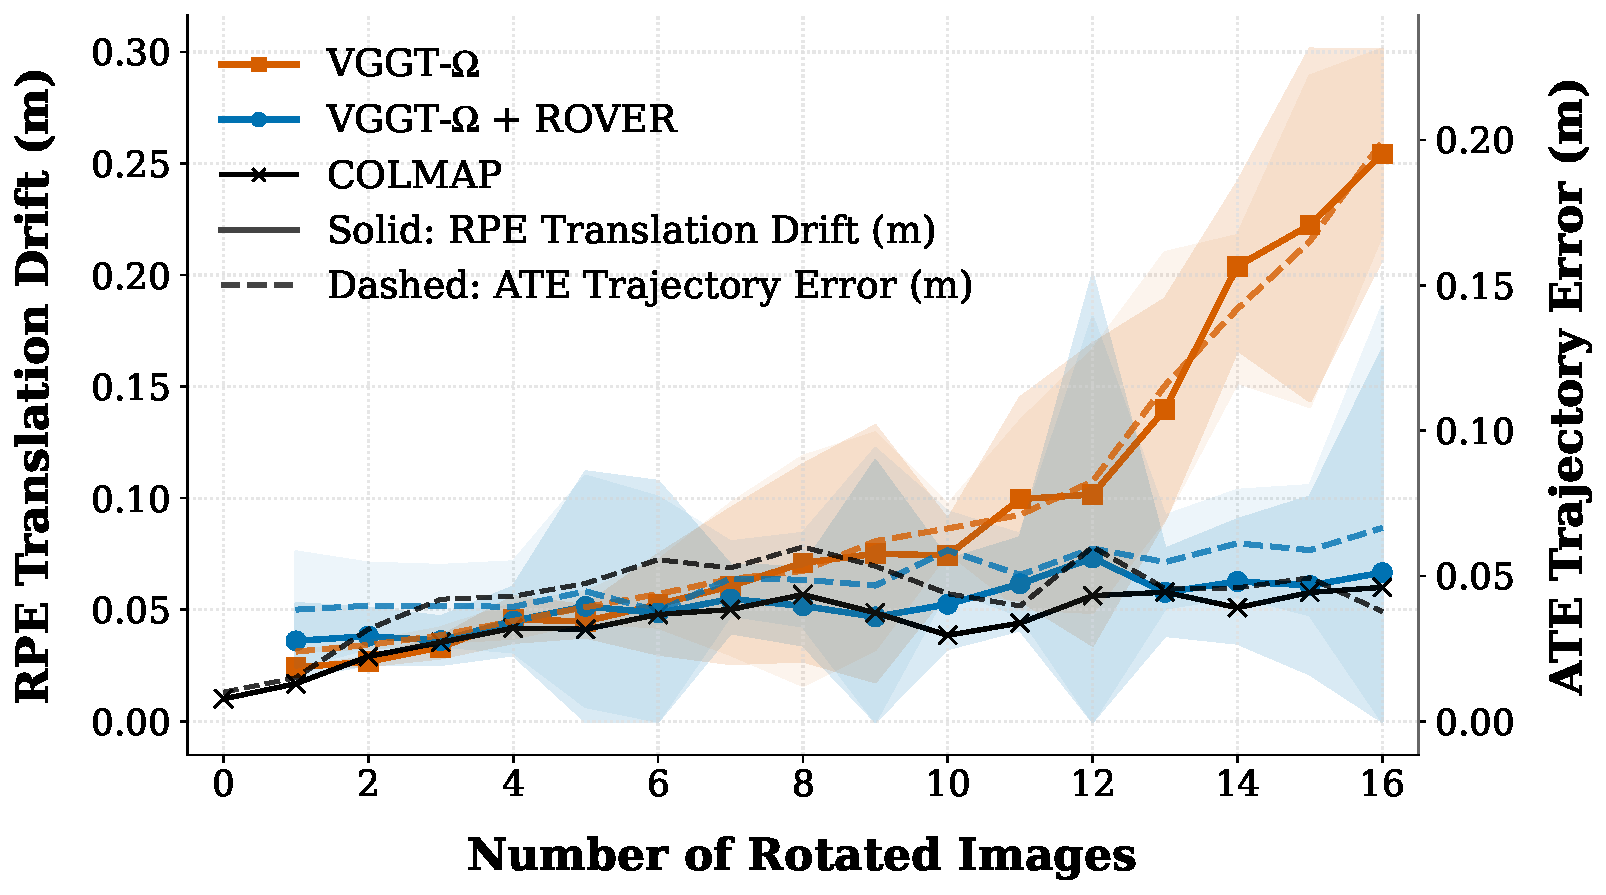
\includegraphics[width=0.75\linewidth]{supplementary_figures/model_comparison.pdf}
    \caption{RPE translation and ATE trajectory error with increasing fraction of rotated input images, comparing ROVER with VGGT-$\Omega$, base model VGGT-$\Omega$ and COLMAP}
    \label{fig:rover_trajectory}
\end{figure}
\subsection{Latency and Computational Overhead of ROVER}
\renewcommand{\arraystretch}{1.2}
\begin{table}[H]
\centering
\small
\setlength{\tabcolsep}{6pt}
\caption{Latency and computational overhead of ROVER across VGGT, VGGT-$\Omega$, $\pi^3$, MapAnything and DepthAnything3}
\label{tab:rover_latency}
\begin{tabular}{lcccc}
\toprule
\textbf{Model} &
\textbf{Base Latency} &
\textbf{ROVER Correction} &
\textbf{Total Latency} &
\textbf{Added Overhead} \\
& \textbf{(seconds)} &
\textbf{(seconds)} &
\textbf{(seconds)} &
\textbf{(\%)} \\
\midrule
VGGT
& \valrow{1.769}{0.017}
& \valrow{0.433}{0.004}
& \valrow{2.169}{0.027}
& $+24.5\%$ \\

VGGT-$\Omega$
& \valrow{1.400}{0.006}
& \valrow{0.424}{0.003}
& \valrow{1.786}{0.009}
& $+30.3\%$ \\

$\pi^3$
& \valrow{1.296}{0.004}
& \valrow{0.428}{0.001}
& \valrow{1.701}{0.034}
& $+33.0\%$ \\

MapA
& \valrow{5.789}{0.038}
& \valrow{0.430}{0.004}
& \valrow{6.203}{0.033}
& $+7.4\%$ \\

DA3
& \valrow{2.003}{0.010}
& \valrow{0.431}{0.003}
& \valrow{2.444}{0.016}
& $+21.5\%$ \\
\bottomrule
\end{tabular}
\end{table}

Additionally we compute latency introduced by the ROVER in ~\Cref{tab:rover_latency} for $16$ images. For all of the models, the introduced latency remains less than $50\%$ of the base model latency, with the observed overhead ranging from $7.4\%$ to $33.0\%$. The ROVER correction itself incurs a nearly constant latency of approximately $0.43$ seconds across all models, irrespective of the underlying model. The relative overhead decreases for models with higher base latency, with Map-Anything incurring only $7.4\%$ overhead, demonstrating the low computational cost of ROVER.


\section{Algorithm}
\label{sec:algorithm}
% ------------------------------------------------------------

% \Badri{All tables should be cited, All sections should be written properly. All tables should be cited in ascending order, meaning if table A is shown before table B and then table A should also be cited before table B }

% \Badri{Fig \Cref{fig:denoise-examples}, the red boxes should be on both colum, also the heading for each row is should be wrriten properly, current all font is small, font style is different. This is very lazy work}

% \Badri{ Fig \Cref{fig:pointcloud_comparison} currently only shows results for vggt, please include results for other models (specially for vggt-omega). They either can be same scene but different models (like in main paper) or can be different scenes as well}

\renewcommand{\algorithmicrequire}{\textbf{Input:}}
\renewcommand{\algorithmicensure}{\textbf{Output:}}

\begin{algorithm}[!htb]
\caption{Rendering-Based Rotated Image Generation}
\label{alg:rotation_generation}
\begin{algorithmic}[1]
    \REQUIRE Multi-view images $\{\mathbf{I}_i\}$, poses $\{\mathbf{P}_i\}$, quality threshold $\tau$
    \ENSURE Rotated images $\{\mathbf{I}_i^{\theta_i}\}$
    \STATE Fit 3DGS representation $\mathcal{G}$ on $\{\mathbf{I}_i, \mathbf{P}_i\}$
           % \COMMENT{Assess reconstruction quality}
    \FOR{each view $i$}
        \STATE Sample $\theta_i \sim \mathcal{U}(0^\circ, 360^\circ)$
        \STATE Compute $\mathbf{P}_i^{\theta_i}$
        \STATE $\mathbf{I}_i^{\theta_i} \leftarrow \mathrm{Render}(\hat{\mathcal{G}},\, \mathbf{P}_i^{\theta_i})$
        \STATE $q \leftarrow \mathrm{VisualQuality\text{-}R1}(\mathbf{I}_i^{\theta_i})$
        \IF{$q \leq \tau$}
            \STATE $\mathbf{I}_i^{\theta_i} \leftarrow \mathrm{Difix3D\_Denoise}(\mathbf{I}_i^{\theta_i})$  \IF{$\mathrm{VisualQuality\text{-}R1}(\mathbf{I}_i^{\theta_i}) \leq \tau$}
                \STATE Exclude view $i$ from evaluation
            \ENDIF
        \ENDIF
    \ENDFOR
    \FOR{each image $\mathbf{I} \in \{\mathbf{I}_i^{\theta_i}\}$}
        \STATE Manually verify $\mathbf{I}$ and remove it from the set if visible artifacts are observed
    \ENDFOR
\end{algorithmic}
\end{algorithm}

\begin{algorithm}[!htb]
\caption{ROVER: Variance-based Canonical Orientation Estimation}
\label{alg:var_alg}
\begin{algorithmic}[1]
    \REQUIRE Image $\mathbf{I}$, frozen DINOv2 encoder $\phi$, 
             coarse step $\Delta_c = 15^\circ$, fine window 
             $\Delta_f = 7^\circ$
    \ENSURE Canonicalized image $\mathbf{I}^{\mathrm{can}}$ 
            with estimated roll $\hat{\theta}$

    \STATE \textit{// Coarse stage}
    \STATE $\Theta_\text{coarse} \leftarrow 
           \{k \cdot \Delta_c \mid k = 1, \ldots, 
           \lfloor 360^\circ / \Delta_c \rfloor\}$
    \FOR{each $\theta \in \Theta_\text{coarse}$}
        \STATE $V(\theta) \leftarrow \textsc{EmbedVar}^{\ref{alg:embedvar}}
               (\mathbf{I}, \theta, \phi)$
    \ENDFOR
    \STATE $\theta_c \leftarrow 
           \arg\max_{\theta \in \Theta_\text{coarse}} V(\theta)$

    \STATE \textit{// Fine stage}
    \STATE $\Theta_\text{fine} \leftarrow 
           \{\theta_c + \delta \mid \delta \in 
           [-\Delta_f, \Delta_f],\, \delta \in \mathbb{Z}\}$
    \FOR{each $\theta \in \Theta_\text{fine}$}
        \STATE $V(\theta) \leftarrow \textsc{EmbedVar}^{\ref{alg:embedvar}}
               (\mathbf{I}, \theta, \phi)$
    \ENDFOR
    \STATE $\hat{\theta} \leftarrow 
           \arg\max_{\theta \in \Theta_\text{fine}} V(\theta)$

    \STATE \textit{// Canonicalization}
    \STATE $\mathbf{I}^{\mathrm{can}} \leftarrow 
           \mathrm{Rotate}(\mathbf{I},\, -\hat{\theta})$
    \RETURN $\mathbf{I}^{\mathrm{can}},\, \hat{\theta}$
\end{algorithmic}
\end{algorithm}

\begin{algorithm}[!htb]
\caption{\textsc{EmbedVar}: Patch Embedding Variance Computation}
\label{alg:embedvar}
\begin{algorithmic}[1]
    \REQUIRE Image $\mathbf{I}$, candidate orientation $\theta$, 
             frozen DINOv2 encoder $\phi$
    \ENSURE Patch embedding variance $V(\theta)$
    \STATE $\mathbf{Z}_\theta \leftarrow 
           \phi(\mathrm{Rotate}(\mathbf{I}, \theta))$
           \COMMENT{$M$ patch embeddings $\in \mathbb{R}^D$}
    \STATE $\bar{\mathbf{z}}^\theta \leftarrow 
           \frac{1}{M}\sum_{j=1}^{M} \mathbf{z}_j^\theta$
           \COMMENT{Mean patch embedding}
    \RETURN $\frac{1}{M}\sum_{j=1}^{M}
            \|\mathbf{z}_j^\theta - 
            \bar{\mathbf{z}}^\theta\|_2^2$
\end{algorithmic}
\end{algorithm}


% \begin{algorithm}[H]
% \caption{Variance-based angle detection}
% \label{alg:var_alg}
% \begin{algorithmic}[1]
%     \REQUIRE Image $\mathbf{I}$, candidate orientation set $\Theta$, frozen DINOv2 encoder $\phi$
%     \ENSURE Rotated image $\mathbf{I}^{\theta^\star}$ with predicted roll $\theta^\star$
%     \FOR{each candidate orientation $\theta \in \Theta$}
%         \STATE $\mathbf{I}^{\theta} \leftarrow \mathrm{Rotate}(\mathbf{I},\, \theta)$
%         \STATE $\mathbf{Z}_{\theta} \leftarrow \phi(\mathbf{I}^{\theta})
%                = \{\mathbf{z}_1^\theta, \ldots, \mathbf{z}_M^\theta\}$
%                \COMMENT{Patch embeddings, $\mathbf{z}_j^\theta \in \mathbb{R}^D$}
%         \STATE $\bar{\mathbf{z}}^\theta \leftarrow
%                \frac{1}{M}\sum_{j=1}^{M} \mathbf{z}_j^\theta$
%                \COMMENT{Embedding centroid}
%         \STATE $V(\theta) \leftarrow
%                \frac{1}{M}\sum_{j=1}^{M}
%                \bigl\|\mathbf{z}_j^\theta - \bar{\mathbf{z}}^\theta\bigr\|_2^2$
%                \COMMENT{Patch-embedding variance}
%     \ENDFOR
%     \STATE $\theta^\star \leftarrow \arg\max_{\theta \in \Theta} V(\theta)$
%     \RETURN $\mathbf{I}^{\theta^\star},\, \theta^\star$
% \end{algorithmic}
% \end{algorithm}


% \begin{algorithm}[H]
% \caption{ROVER: Variance-based Canonical Orientation Estimation}
% \label{alg:var_alg}
% \begin{algorithmic}[1]
%     \REQUIRE Image $\mathbf{I}$, frozen DINOv2 encoder $\phi$, 
%              coarse step $\Delta_c = 15^\circ$, fine window 
%              $\Delta_f = 7^\circ$
%     \ENSURE Canonicalized image $\mathbf{I}^{\mathrm{can}}$ 
%             with estimated roll $\hat{\theta}$

%     \STATE \textit{// Coarse stage}
%     \STATE $\Theta_\text{coarse} \leftarrow 
%            \{k \cdot \Delta_c \mid k = 1, \ldots, 
%            \lfloor 360^\circ / \Delta_c \rfloor\}$
%     \FOR{each $\theta \in \Theta_\text{coarse}$}
%         \STATE $V(\theta) \leftarrow \textsc{EmbedVar}
%                (\mathbf{I}, \theta, \phi)$
%     \ENDFOR
%     \STATE $\theta_c \leftarrow 
%            \arg\max_{\theta \in \Theta_\text{coarse}} V(\theta)$

%     \STATE \textit{// Fine stage}
%     \STATE $\Theta_\text{fine} \leftarrow 
%            \{\theta_c + \delta \mid \delta \in 
%            [-\Delta_f, \Delta_f],\, \delta \in \mathbb{Z}\}$
%     \FOR{each $\theta \in \Theta_\text{fine}$}
%         \STATE $V(\theta) \leftarrow \textsc{EmbedVar}
%                (\mathbf{I}, \theta, \phi)$
%     \ENDFOR
%     \STATE $\hat{\theta} \leftarrow 
%            \arg\max_{\theta \in \Theta_\text{fine}} V(\theta)$

%     \STATE \textit{// Canonicalization}
%     \STATE $\mathbf{I}^{\mathrm{can}} \leftarrow 
%            \mathrm{Rotate}(\mathbf{I},\, -\hat{\theta})$
%     \RETURN $\mathbf{I}^{\mathrm{can}},\, \hat{\theta}$
% \end{algorithmic}
% \end{algorithm}


% \begin{algorithm}[H]
% \caption{\textsc{EmbedVar}: Patch Embedding Variance Computation}
% \label{alg:embedvar}
% \begin{algorithmic}[1]
%     \REQUIRE Image $\mathbf{I}$, candidate orientation $\theta$, 
%              frozen DINOv2 encoder $\phi$
%     \ENSURE Patch embedding variance $V(\theta)$
%     \STATE $\mathbf{Z}_\theta \leftarrow 
%            \phi(\mathrm{Rotate}(\mathbf{I}, \theta))$
%            \COMMENT{$M$ patch embeddings $\in \mathbb{R}^D$}
%     \STATE $\bar{\mathbf{z}}^\theta \leftarrow 
%            \frac{1}{M}\sum_{j=1}^{M} \mathbf{z}_j^\theta$
%            \COMMENT{Mean patch embedding}
%     \RETURN $\frac{1}{M}\sum_{j=1}^{M}
%             \|\mathbf{z}_j^\theta - 
%             \bar{\mathbf{z}}^\theta\|_2^2$
% \end{algorithmic}
% \end{algorithm}


Algorithm~\Cref{alg:rotation_generation} provides the pseudocode for controlled rotation synthesis. We first fit a 3DGS representation to each multi-view captured image set. We then sample an angle $\theta \sim \mathcal{U}(0^\circ, 360^\circ)$, render the corresponding rolled image, and score its reconstruction quality $q$ with VisualQuality-R1 \citep{wu2026visualquality}. Captures falling below the predefined threshold $\tau$ are denoised with Difix3D single-step denoiser to remove artifacts, after which the remaining scenes are rendered directly. The renderings are scored again with reconstruction quality $q$ with VisualQuality-R1 to remove images with obvious artifacts. A final manual pass removes images with any residual artifacts.
Orientation is then recovered through (Algorithm~\Cref{alg:var_alg}). For every candidate orientation $\theta\in\Theta$ in a predefined discrete set $\Theta=\{0^\circ,\delta,\ldots,360^\circ-\delta\}$, the input image is rotated by $\theta$ and passed through the frozen DINOv2 encoder $\phi$ to obtain the corresponding patch embeddings,
$\mathbf{Z}_{\theta}=\phi(\mathbf{I}^{\theta})=\{\mathbf{z}_1^\theta,\mathbf{z}_2^\theta,\ldots,\mathbf{z}_M^\theta\}$,
where $\mathbf{I}^{\theta}$ denotes the image rotated by $\theta$, and $\mathbf{z}_j^\theta\in\mathbb{R}^D$ denotes the embedding corresponding to the $j$-th image patch. Each candidate orientation is scored by the variance of its patch embeddings about their centroid,
$V(\theta)=\frac{1}{M}\sum_{j=1}^{M}\left\|\mathbf{z}_j^\theta-\bar{\mathbf{z}}^\theta\right\|_2^2$,
where $\bar{\mathbf{z}}^\theta=\frac{1}{M}\sum_{j=1}^{M}\mathbf{z}_j^\theta$ is the centroid of the patch embeddings. Since the backbone is pre-trained predominantly on upright imagery, patch features are most strongly differentiated at the canonical orientation and collapse toward the centroid as the rotation departs from it. The orientation estimation operator is therefore defined as
$
E(\mathbf{I})=\arg\max_{\theta\in\Theta}V(\theta),
$
and the maximizing candidate gives the predicted roll. We use DINOv2 embeddings to determine the canonical orientation in our approach. Previous works \citep{cuttano2026insid3} points out that DINOv3 features can exhibit spurious correspondences between image pairs regardless of their semantic similarity. In particular, feature similarities between semantically unrelated images exhibit systematic activations aligned with absolute spatial coordinates, indicating a strong positional bias. This positional bias in DINOv3 hinders its ability to accurately identify canonical rotation angle using our variance-maximization approach which makes DINOv2 as an encoder $\phi$.

\section{Orientation Variance Plots}
\label{sec:ROVER_empirical_plots}

We include plot of variance of token embeddings w.r.t. the image orientation in \cref{fig:variance_vs_angle_all_datasets} for datasets 7-Scenes, NRGB-D, Tanks and Temples and RotMV. To analyze the orientation dependence of DINOv2 representations, we synthetically rotate each canonical image over \(0^\circ\!-\!360^\circ\) in \(15^\circ\) increments and compute the same patch-token spatial variance used by our method, excluding padded regions introduced by rotation. To isolate orientation-dependent changes from image-specific differences in absolute variance, each image’s variance curve is independently min–max normalized across candidate rotations before aggregation. 

\Cref{fig:variance_vs_angle_all_datasets} shows the mean normalized variance across all images, with \(\pm 1\) standard deviation. We use upright images here to calculate variance. We show that for all datasets, the variance of token embeddings consistently achieves its maximum value at canonical orientation ($0^\circ$ in this case, as we used upright images), while non-canonical rotations produce substantially lower values with weaker secondary peaks near multiples of \(90^\circ\). This supports the use of DINOv2 patch-embedding variance as a reliable signal for identifying canonical upright orientation. 


\begin{figure*}[!ht]
    \centering
    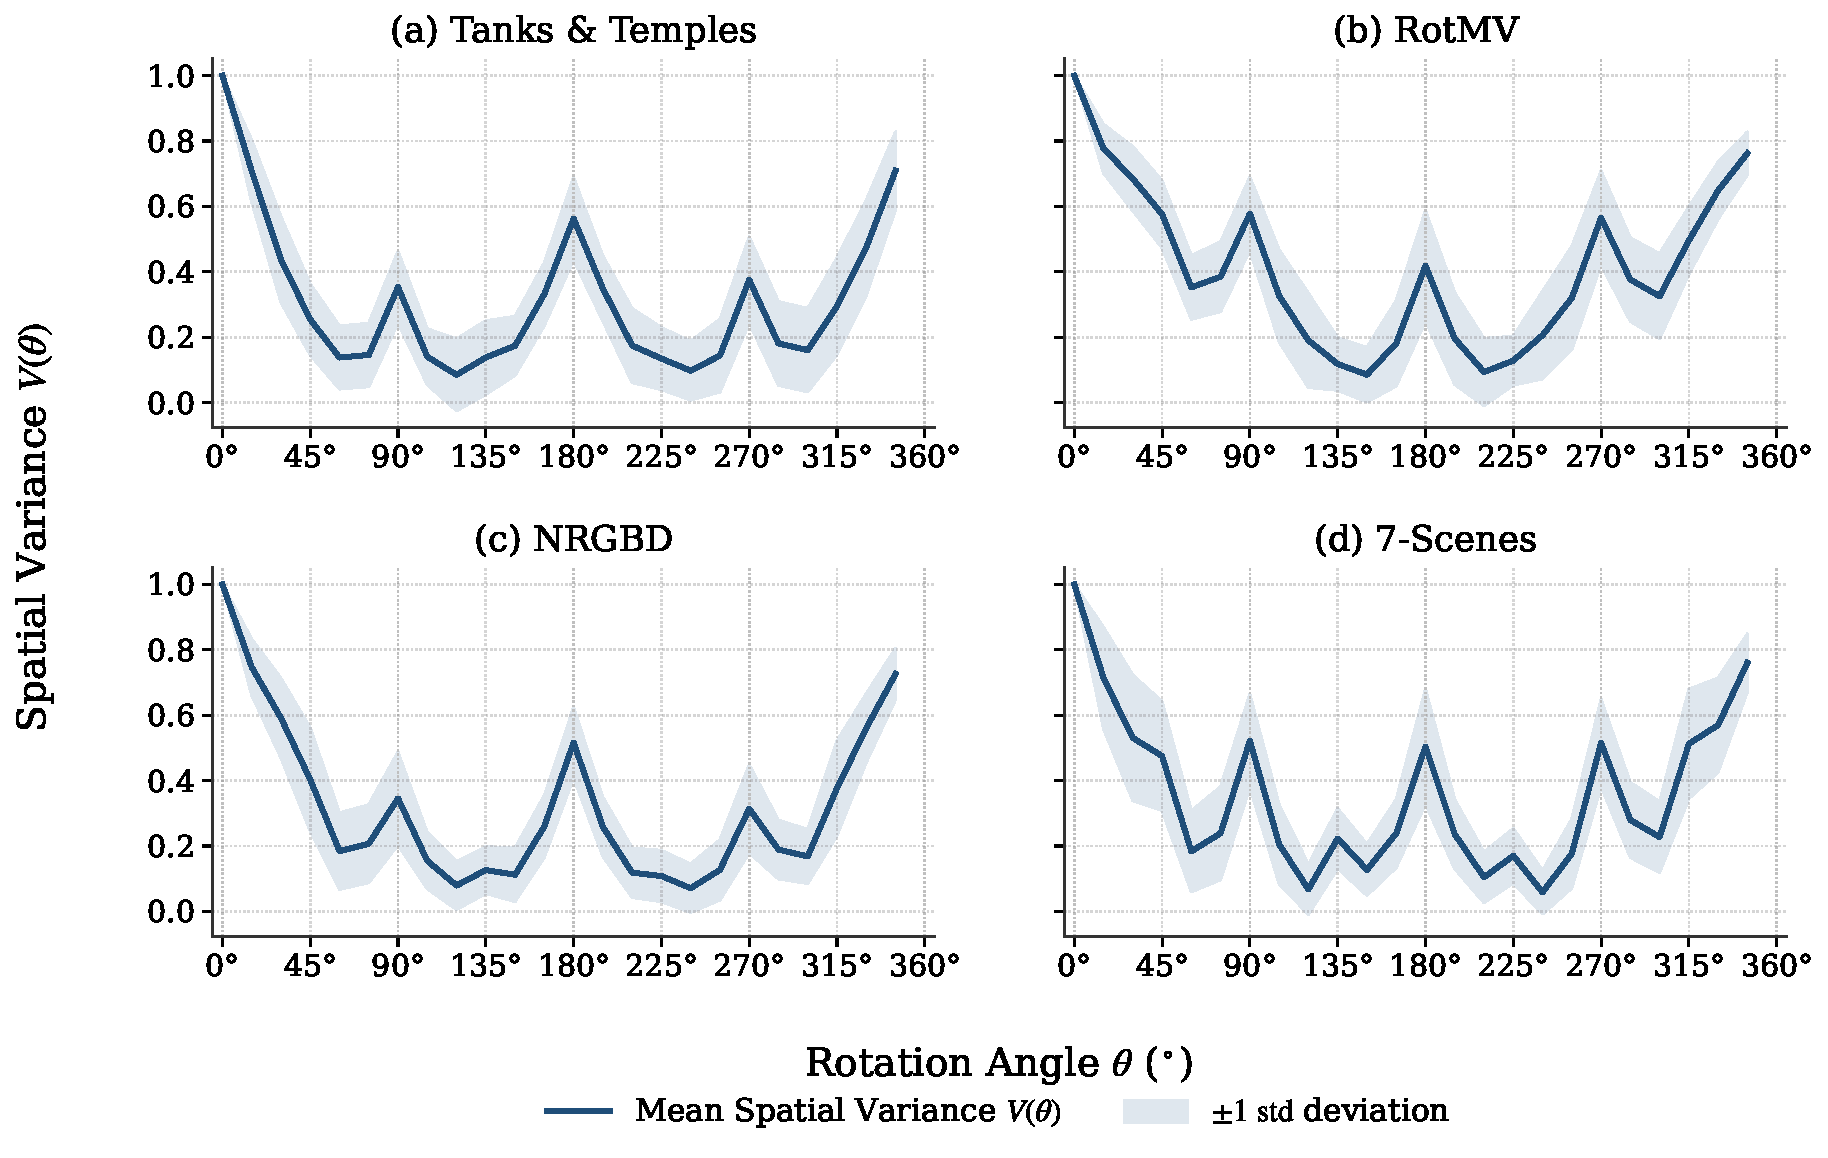
\includegraphics[width=0.98\textwidth]{supplementary_figures/variance_plots/all_datasets_grid_2x2.pdf}
    \caption{
        Variance as a function of rotation angle across the RotMV, NRGB-D, 7-Scenes, and Tanks and Temples datasets. We observe that ROVER consistently helps estimate the upright orientation of the images 
    }
    \label{fig:variance_vs_angle_all_datasets}
\end{figure*}
We also plot the variance for images rotated by $225^\circ$ in \cref{fig:variance_vs_angle_225_deg} for Tanks and Temples, NRGB-D and 7-Scenes. Each rotated image is further rotated by candidate angles over $[0^\circ, 360^\circ)$ in $15^\circ$ increments, and the variance is maximized by the candidate that restores the upright orientation ($135^\circ$). We plot the mean normalized variance against the estimated rotation $\theta = 360^\circ - $ candidate, so the peak appears at $\theta = 225^\circ$ for all three datasets and the correction is simply a rotation by $-\theta$. In the upright setting, the peak occurs at $0^\circ$, where no rotation (and hence no padding) is applied, so one could argue the peak is simply caused by the absence of padding. Here, leaving the image unrotated ($\phi = 0^\circ$) does not give the maximum; instead, the peak occurs at $\phi = 135^\circ$, which adds padding(because of the rotation) but restores the upright view. This shows that the variance peak is driven by the upright orientation of the image content, not by the padding.

\begin{figure*}[!ht]
    \centering
    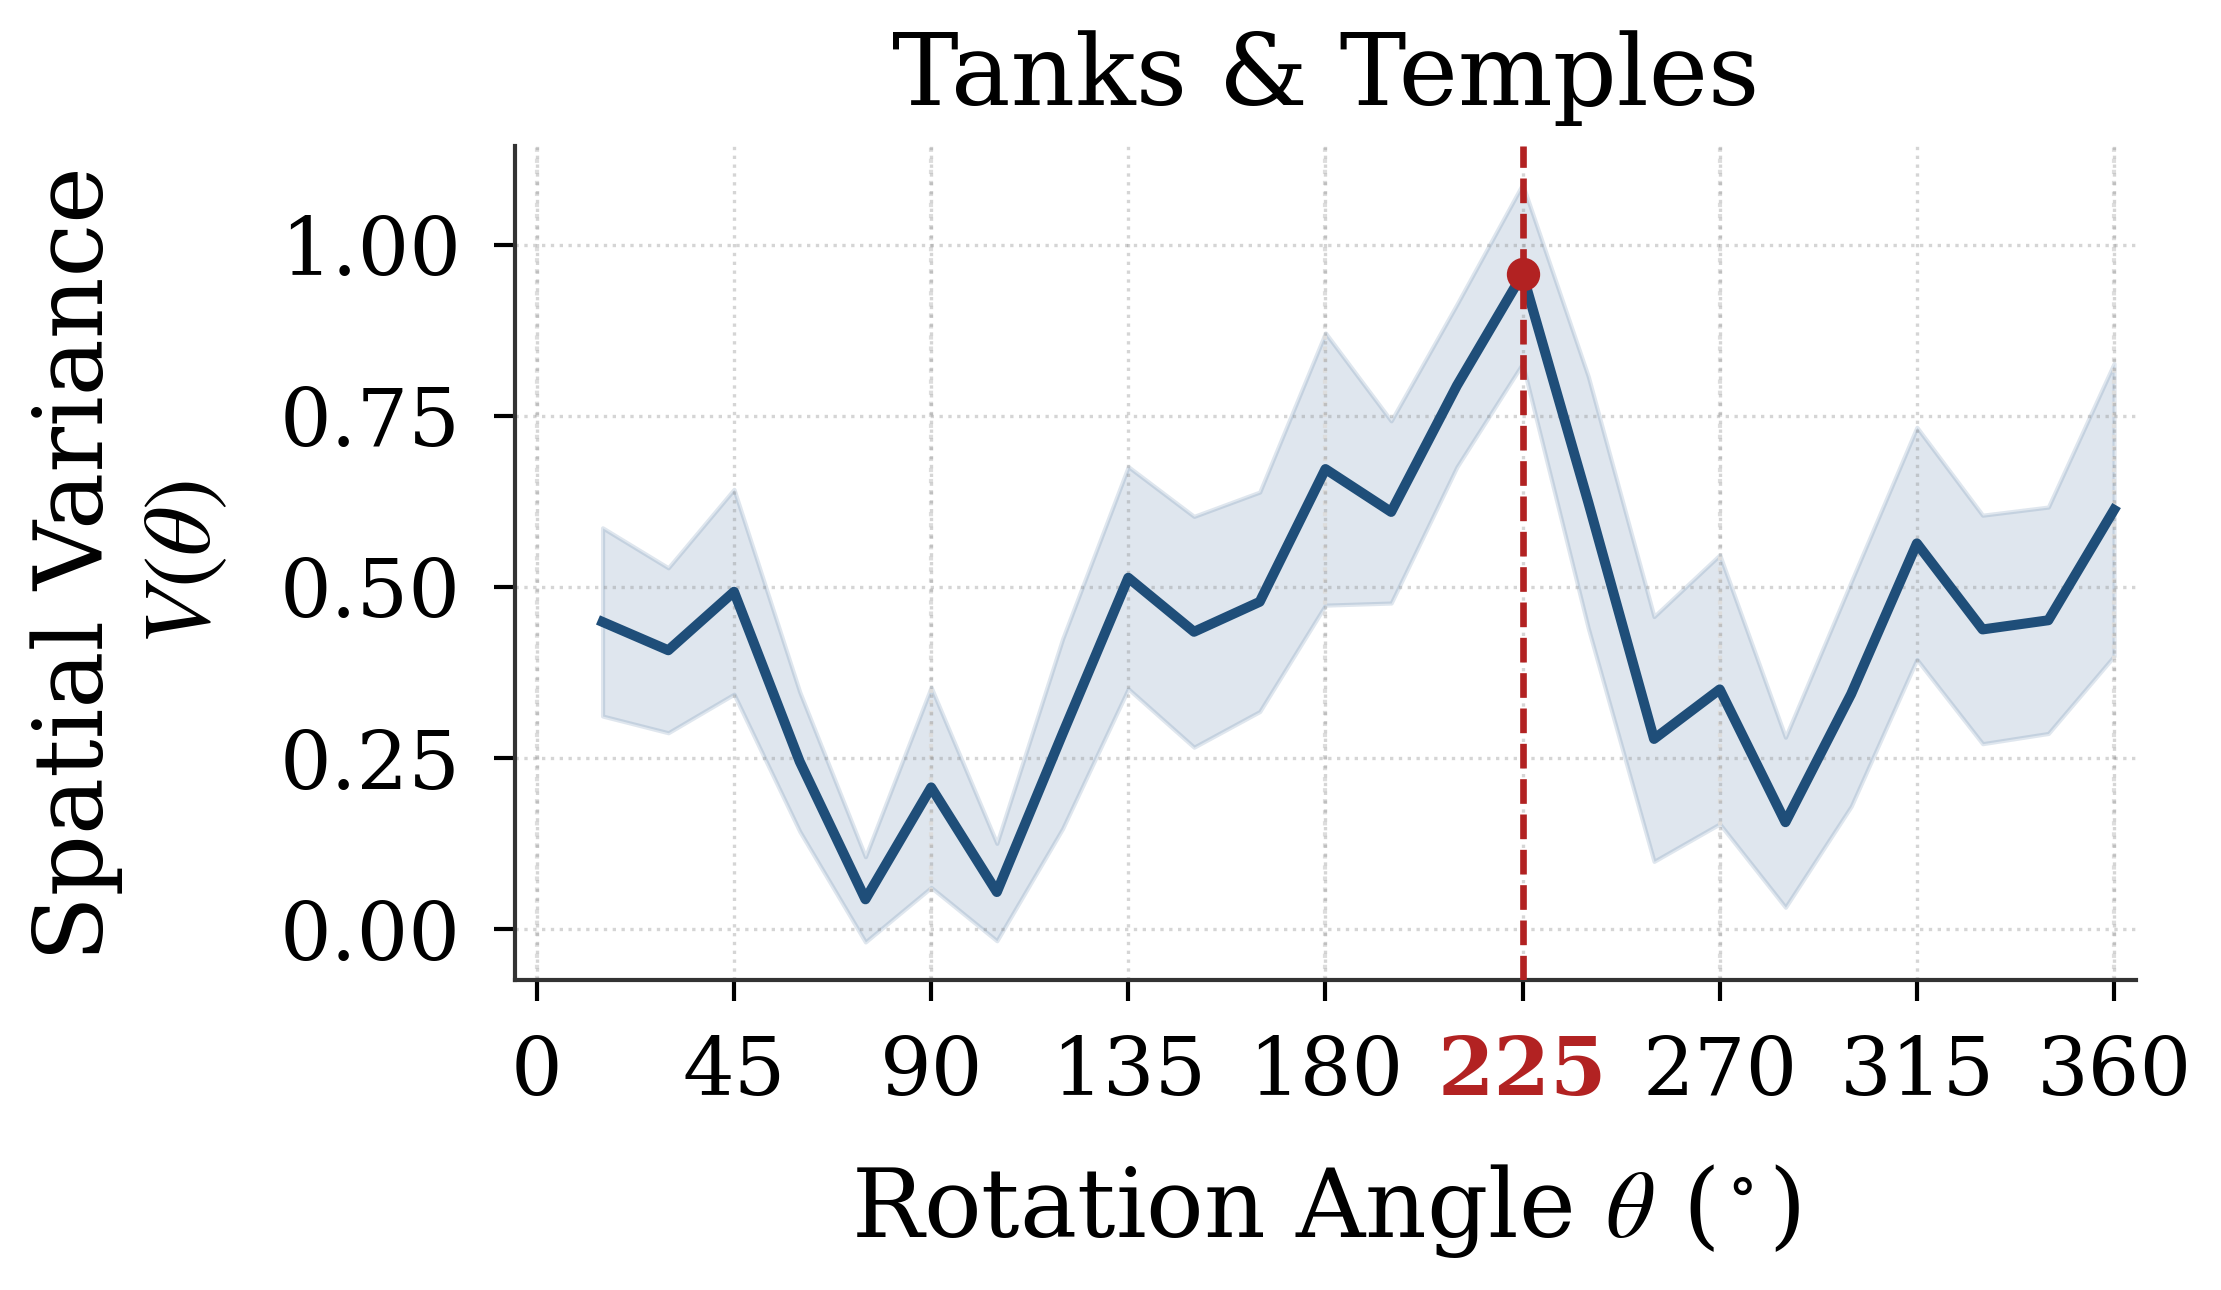
\includegraphics[width=0.325\textwidth]{supplementary_figures/variance_plots/all_scenes_variance_vs_angle_tnt_225.png}\hfill
    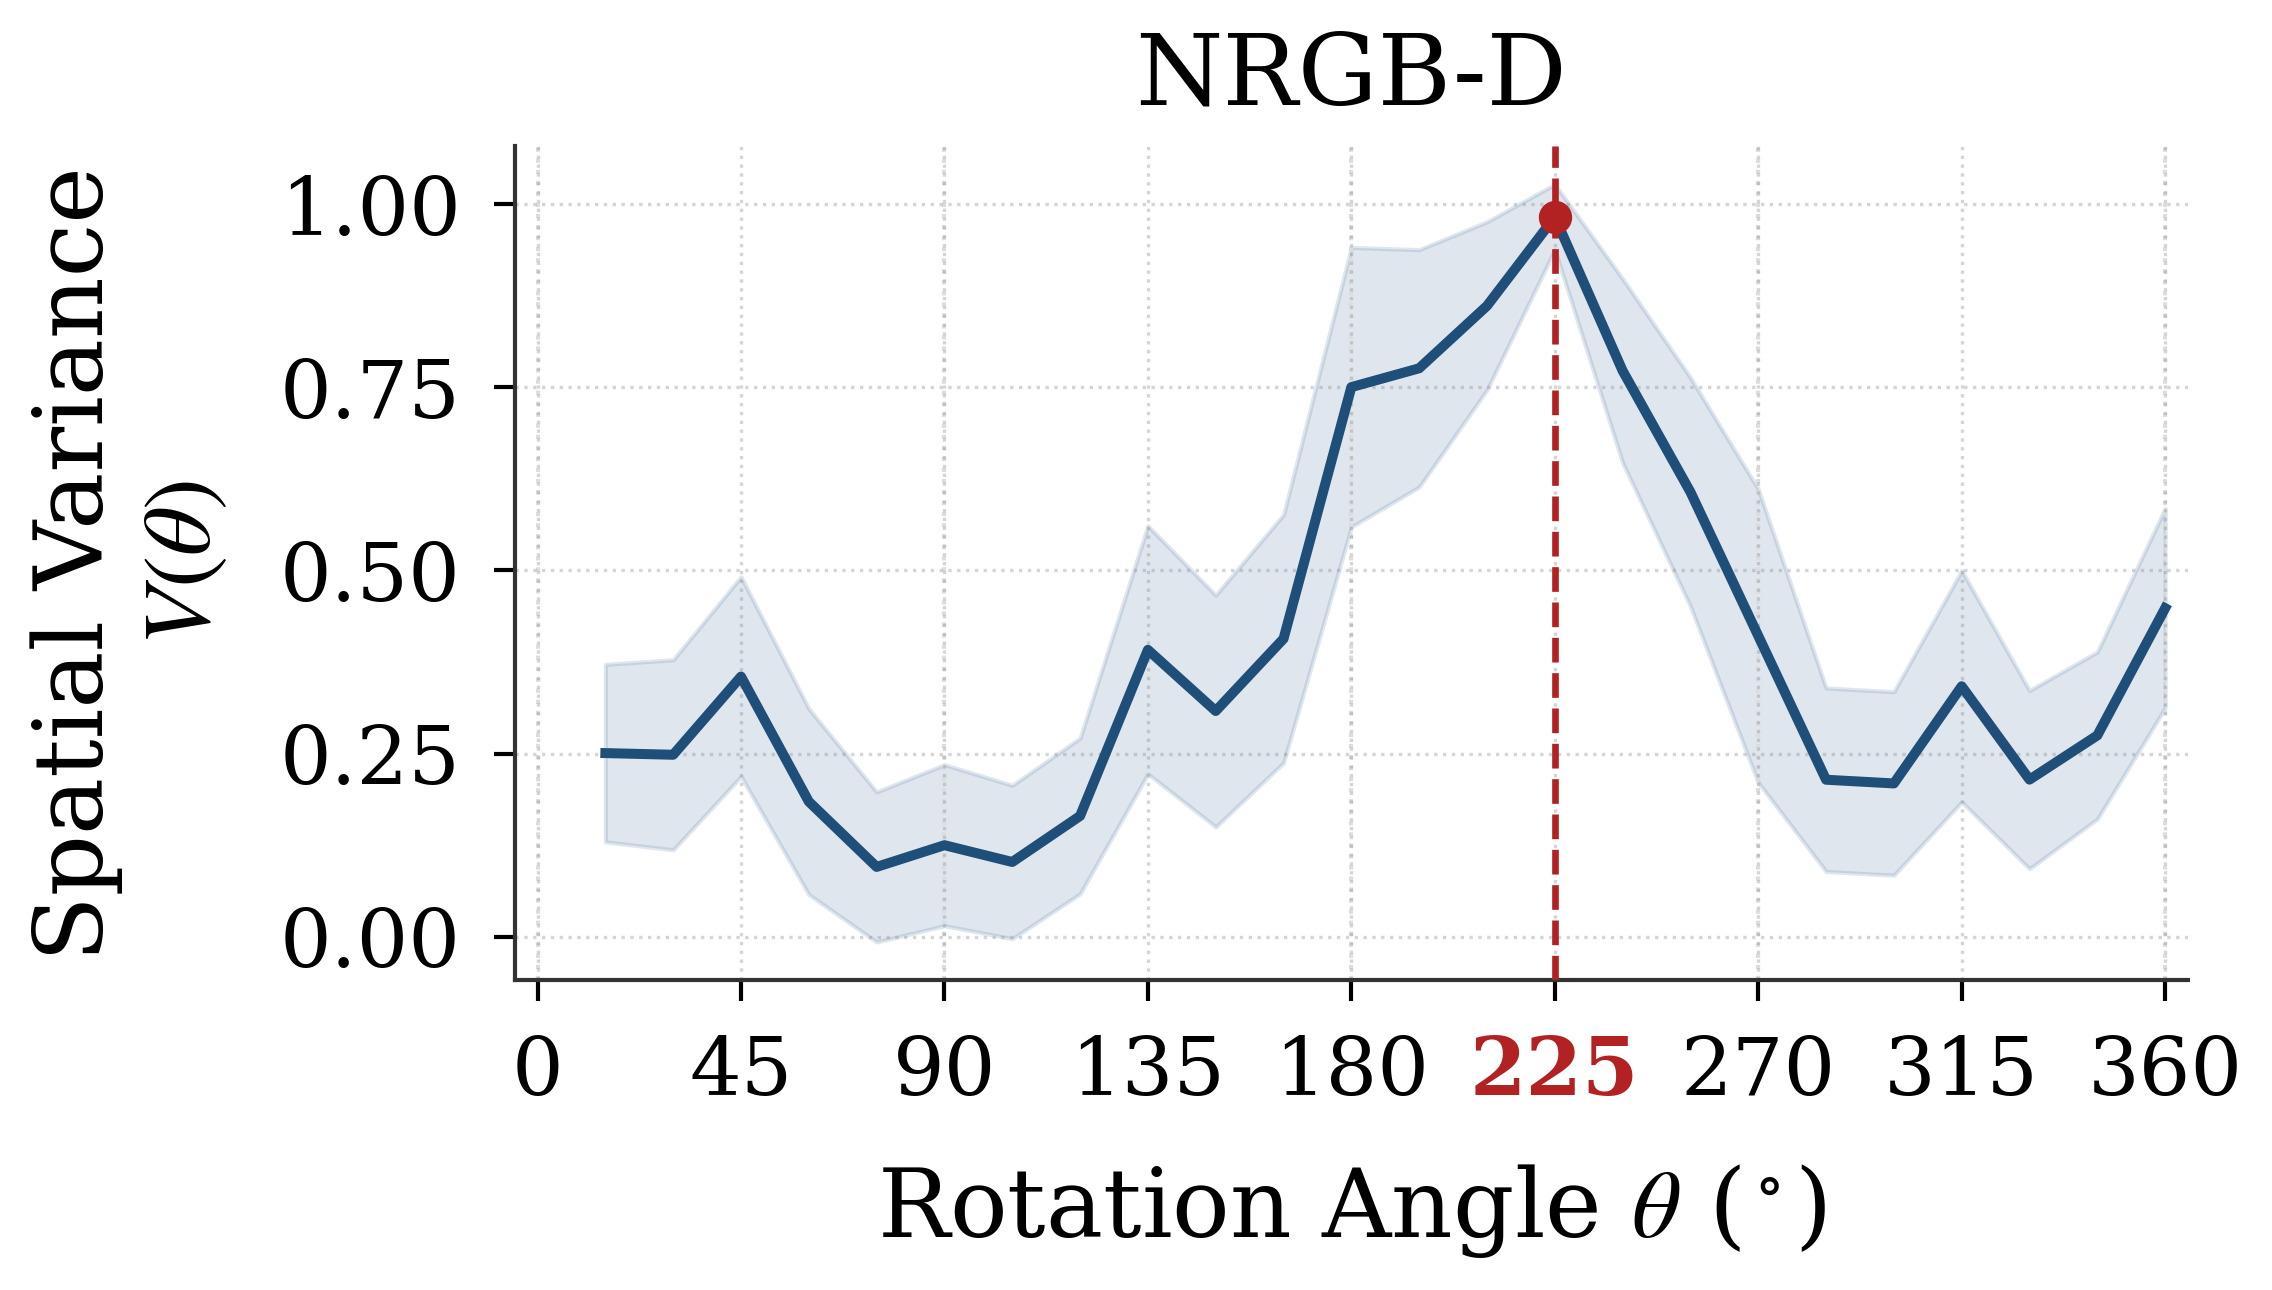
\includegraphics[width=0.325\textwidth]{supplementary_figures/variance_plots/all_scenes_variance_vs_angle_nrgbd.png}\hfill
    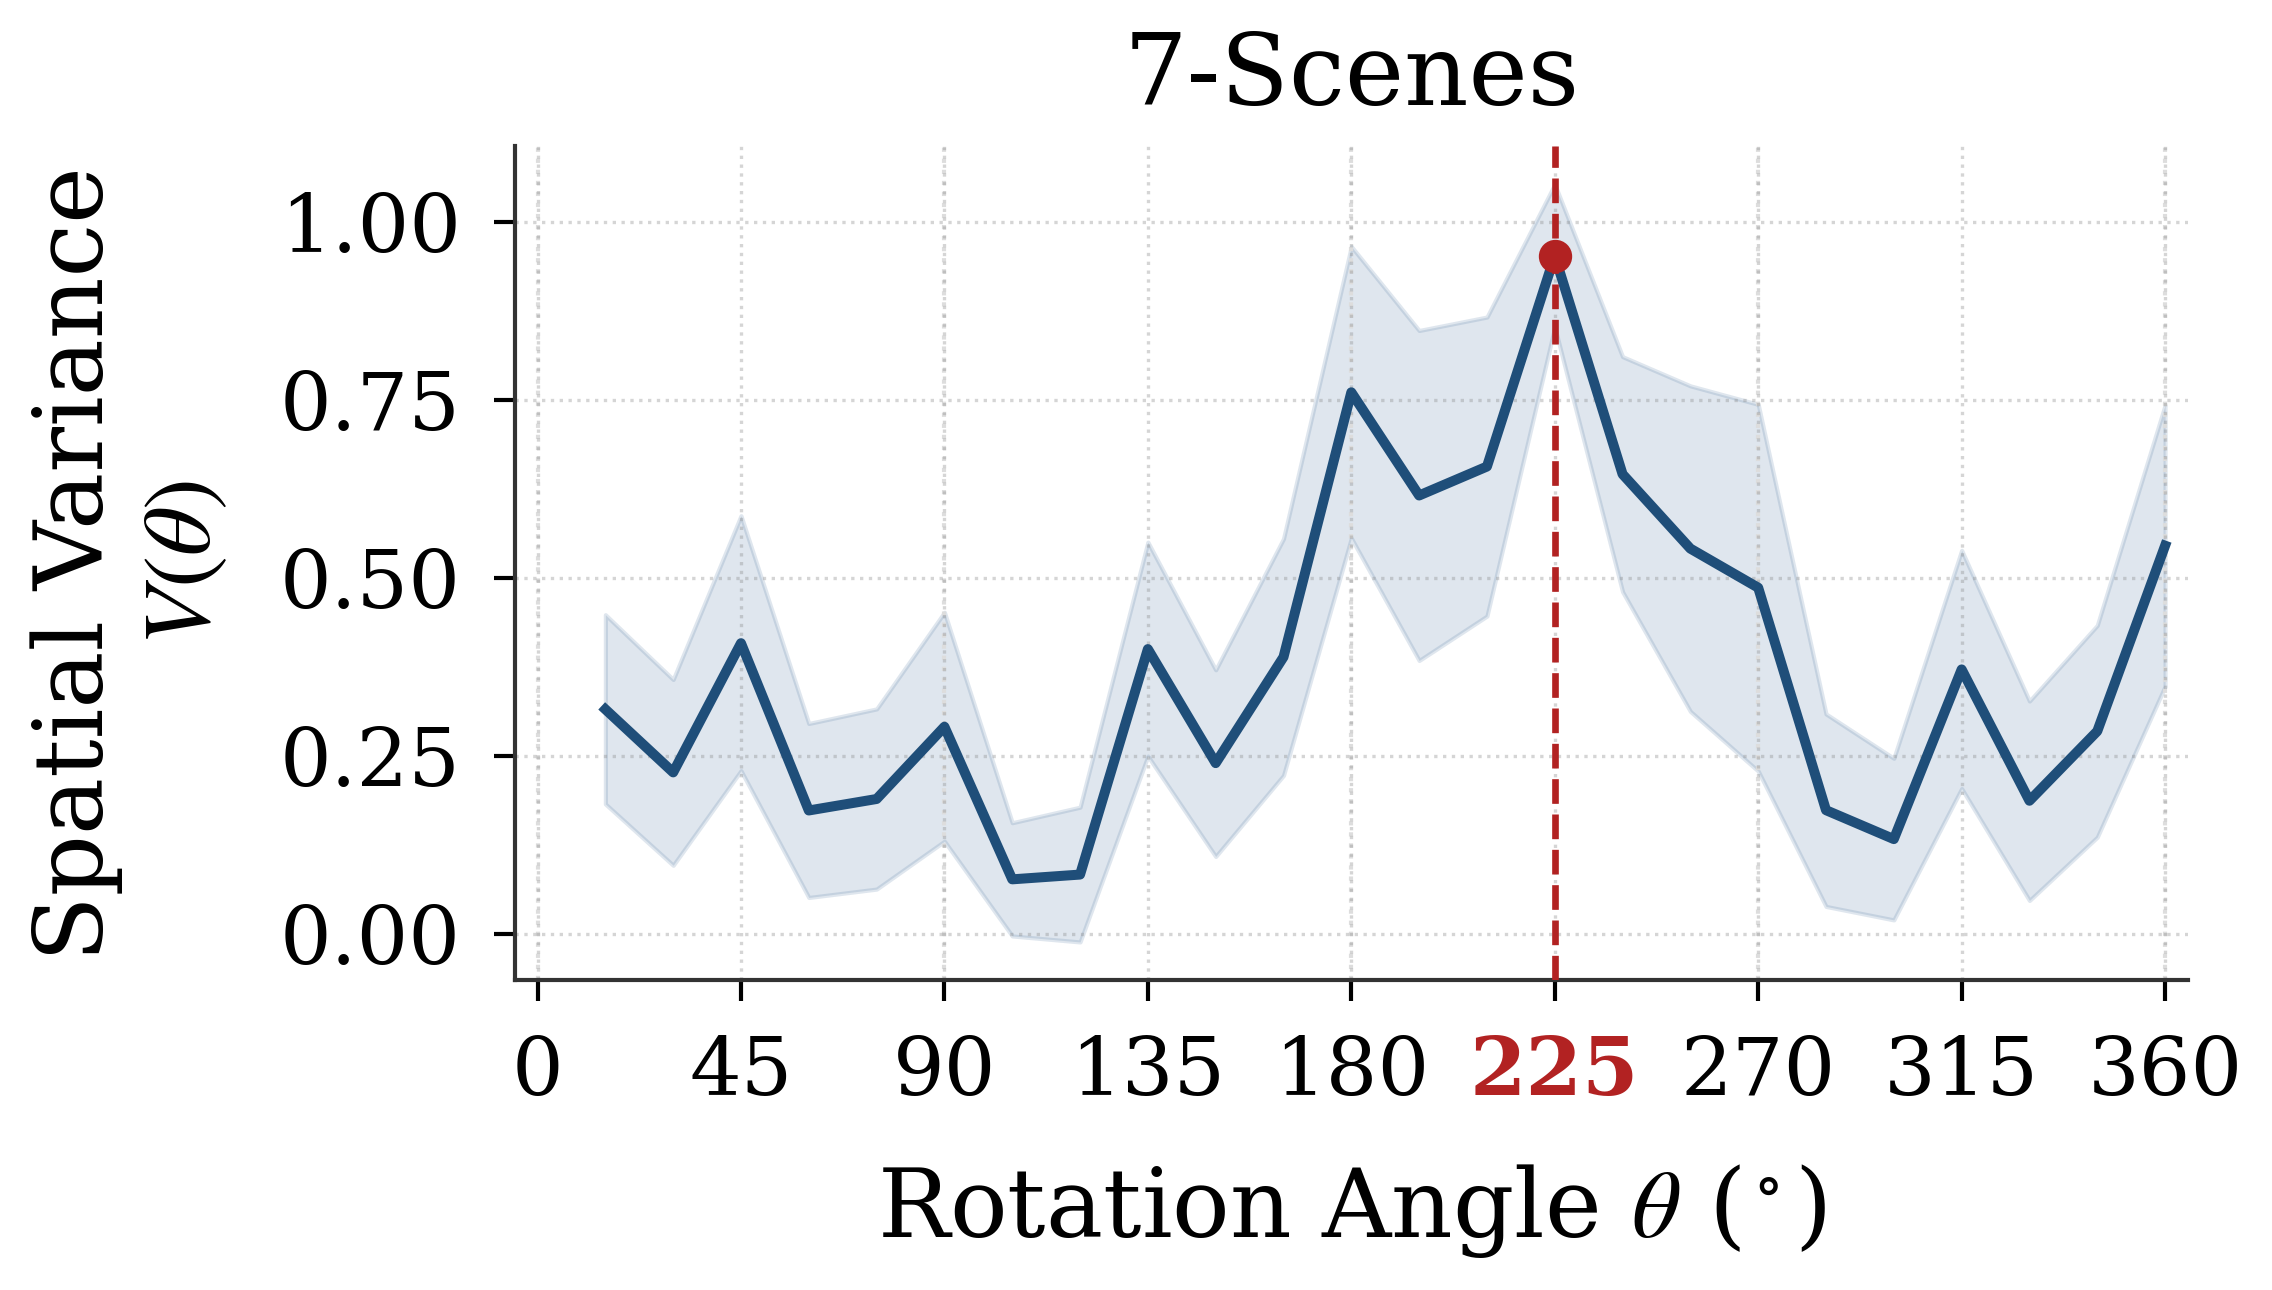
\includegraphics[width=0.325\textwidth]{supplementary_figures/variance_plots/all_scenes_variance_vs_angle_7scenes_225.png}
\caption{ROVER recovers the true rotation angle. Input images are rotated by $225^\circ$ from their upright orientation. We plot the normalized patch-embedding variance (mean $\pm 1$ std) against the estimated rotation $\theta = 360^\circ - \phi$, where $\phi$ is the candidate correction. The peak (red dashed line) falls at $\theta = 225^\circ$ for all three datasets, so rotating by $-\theta$ restores the upright view.}
    \label{fig:variance_vs_angle_225_deg}
\end{figure*}

% ------------------------------------------------------------
\section{Sensitivity to Limited Pitch Rotations}  % TODO: rename
\label{sec:pose_pitch}
% ------------------------------------------------------------
We additionally evaluate sensitivity to camera rotations about the pitch axis on NRGB-D, 7-Scenes, and Tanks\&Temples in~\Cref{tab:pitch_metrics}. Following the evaluation protocol described in~\Cref{sec:experimental_setup}, we evaluate the four non-zero rotation levels ($25\%$, $50\%$, $75\%$, and $100\%$ rotated views). Selected views are independently assigned a pitch perturbation from $[-5^\circ, +5^\circ]$; the corresponding camera pose is then perturbed and a new view is rendered using~\Cref{sec:rendering_based_rotation}. Large perturbation leads to change in viewpoint of the scene as the camera will point to a different region in the scene unlike roll perturbation thus we restrict the perturbation to limited range. Across this limited range, performance remains close to the upright setting for most models and datasets. For instance, VGGT changes from $0.798$ to $0.796$ N.C. and from $98.36$ to $98.17$ AUC$_{30}$ on NRGB-D, while on Tanks\&Temples the corresponding values change from $0.678$ to $0.671$ and from $91.62$ to $91.20$. Larger variation is observed in some cases, such as $\pi^3$ on Tanks\&Temples, where N.C. decreases from $0.701$ to $0.666$, although pose accuracy remains comparatively stable. Overall, these results indicate sensitivity to small pitch perturbations over the evaluated range.

\renewcommand{\arraystretch}{1.2}
\providecommand{\dd}[2]{\makecell{#1 \\ {\tiny $\pm$ #2}}}

\begin{table}[h]
\centering
\caption{Point-map (N.C., $\uparrow$) and pose (AUC@30, $\uparrow$) accuracy, upright vs.\ rotated about the pitch axis, on NRGBD, 7-Scenes, and Tanks\&Temples.}
\label{tab:pitch_metrics}
\scriptsize
\setlength{\tabcolsep}{3pt}
\resizebox{\linewidth}{!}{%
\begin{tabular}{l *{3}{cc cc}}
\toprule
 & \multicolumn{4}{c}{\textbf{NRGBD}}
 & \multicolumn{4}{c}{\textbf{7-Scenes}}
 & \multicolumn{4}{c}{\textbf{Tanks\&Temples}} \\
\cmidrule(lr){2-5} \cmidrule(lr){6-9} \cmidrule(lr){10-13}

 & \multicolumn{2}{c}{N.C. $\uparrow$}
 & \multicolumn{2}{c}{AUC@30 $\uparrow$}
 & \multicolumn{2}{c}{N.C. $\uparrow$}
 & \multicolumn{2}{c}{AUC@30 $\uparrow$}
 & \multicolumn{2}{c}{N.C. $\uparrow$}
 & \multicolumn{2}{c}{AUC@30 $\uparrow$} \\
\cmidrule(lr){2-3} \cmidrule(lr){4-5}
\cmidrule(lr){6-7} \cmidrule(lr){8-9}
\cmidrule(lr){10-11} \cmidrule(lr){12-13}

\textbf{Method}
& Up. & Rot. & Up. & Rot.
& Up. & Rot. & Up. & Rot.
& Up. & Rot. & Up. & Rot. \\
\midrule

VGGT
& \dd{0.798}{0.031} & \dd{0.796}{0.005} & \dd{98.36}{1.44} & \dd{98.17}{0.38}
& \dd{0.661}{0.038} & \dd{0.662}{0.003} & \dd{85.60}{6.73} & \dd{84.68}{1.23}
& \dd{0.678}{0.054} & \dd{0.671}{0.022} & \dd{91.62}{14.60} & \dd{91.20}{0.79} \\
\addlinespace[3pt]

VGGT-$\Omega$
& \dd{0.827}{0.049} & \dd{0.824}{0.007} & \dd{99.22}{0.57} & \dd{98.84}{0.43}
& \dd{0.670}{0.050} & \dd{0.670}{0.003} & \dd{88.07}{5.80} & \dd{87.05}{1.20}
& \dd{0.684}{0.083} & \dd{0.664}{0.016} & \dd{92.88}{14.29} & \dd{92.79}{0.36} \\
\addlinespace[3pt]

$\pi^3$
& \dd{0.807}{0.077} & \dd{0.805}{0.007} & \dd{96.32}{2.74} & \dd{95.86}{0.56}
& \dd{0.682}{0.050} & \dd{0.683}{0.003} & \dd{85.13}{8.09} & \dd{84.59}{1.36}
& \dd{0.701}{0.056} & \dd{0.666}{0.030} & \dd{94.46}{8.71} & \dd{94.20}{0.86} \\
\addlinespace[3pt]

MapA.
& \dd{0.741}{0.052} & \dd{0.720}{0.012} & \dd{93.86}{3.79} & \dd{93.25}{0.84}
& \dd{0.631}{0.059} & \dd{0.633}{0.010} & \dd{76.22}{15.42} & \dd{75.69}{1.82}
& \dd{0.614}{0.065} & \dd{0.592}{0.030} & \dd{92.48}{3.04} & \dd{91.70}{1.29} \\
\addlinespace[3pt]

DA3
& \dd{0.815}{0.043} & \dd{0.810}{0.009} & \dd{99.77}{0.37} & \dd{99.74}{0.11}
& \dd{0.678}{0.041} & \dd{0.678}{0.004} & \dd{88.14}{5.95} & \dd{87.44}{1.48}
& \dd{0.694}{0.057} & \dd{0.683}{0.024} & \dd{98.45}{1.16} & \dd{97.87}{1.83} \\

\bottomrule
\end{tabular}%
}
\end{table}

\section{Examples of Point Cloud Degradation}

% \Badri{Add additinoal results where we show degradation when all images are rotated with same angle}
We qualitatively illustrate the effect of in-plane roll on point-cloud reconstruction in Figures \Cref{fig:pc_tanks_and_temples}, \Cref{fig:pc_tnt_barn}
\Cref{fig:pc_7scenes_kitchen} 
across VGGT, VGGT-$\Omega$, $\pi^3$, and DepthAnything3 (DA3). Under rotated inputs,
the baseline reconstructions exhibit substantial geometric artifacts, including distorted
structures, misaligned surfaces, and, most prominently, duplicated scene elements, as
highlighted in the zoomed regions. Applying ROVER consistently reduces these artifacts
across the different backbones and produces substantially cleaner and more coherent
point-cloud reconstructions despite the input images being arbitrarily rotated in-plane.

We additionally evaluate the setting where all input images are rotated by the same angle in ~\Cref{fig:uniform_rotation_office}, preserving their relative orientations. Surprisingly, models still fail to reconstruct the scene, demonstrating that the degradation is not caused by relative pose ambiguity between views but by a learned prior on absolute image orientation the model simply does not expect to see images that deviate from upright.

%%%%%%%%%%%%%%%%%%%%%%%%%%%%%%%%%%%%%%%%%%%%%%%%=========================================================================
% PAGE 1: Tanks & Temples (Truck, Church) + 7-Scenes (Office)
% =========================================================================
\begin{figure*}[p]
\centering

% --- Dataset 1: Tanks & Temples ---
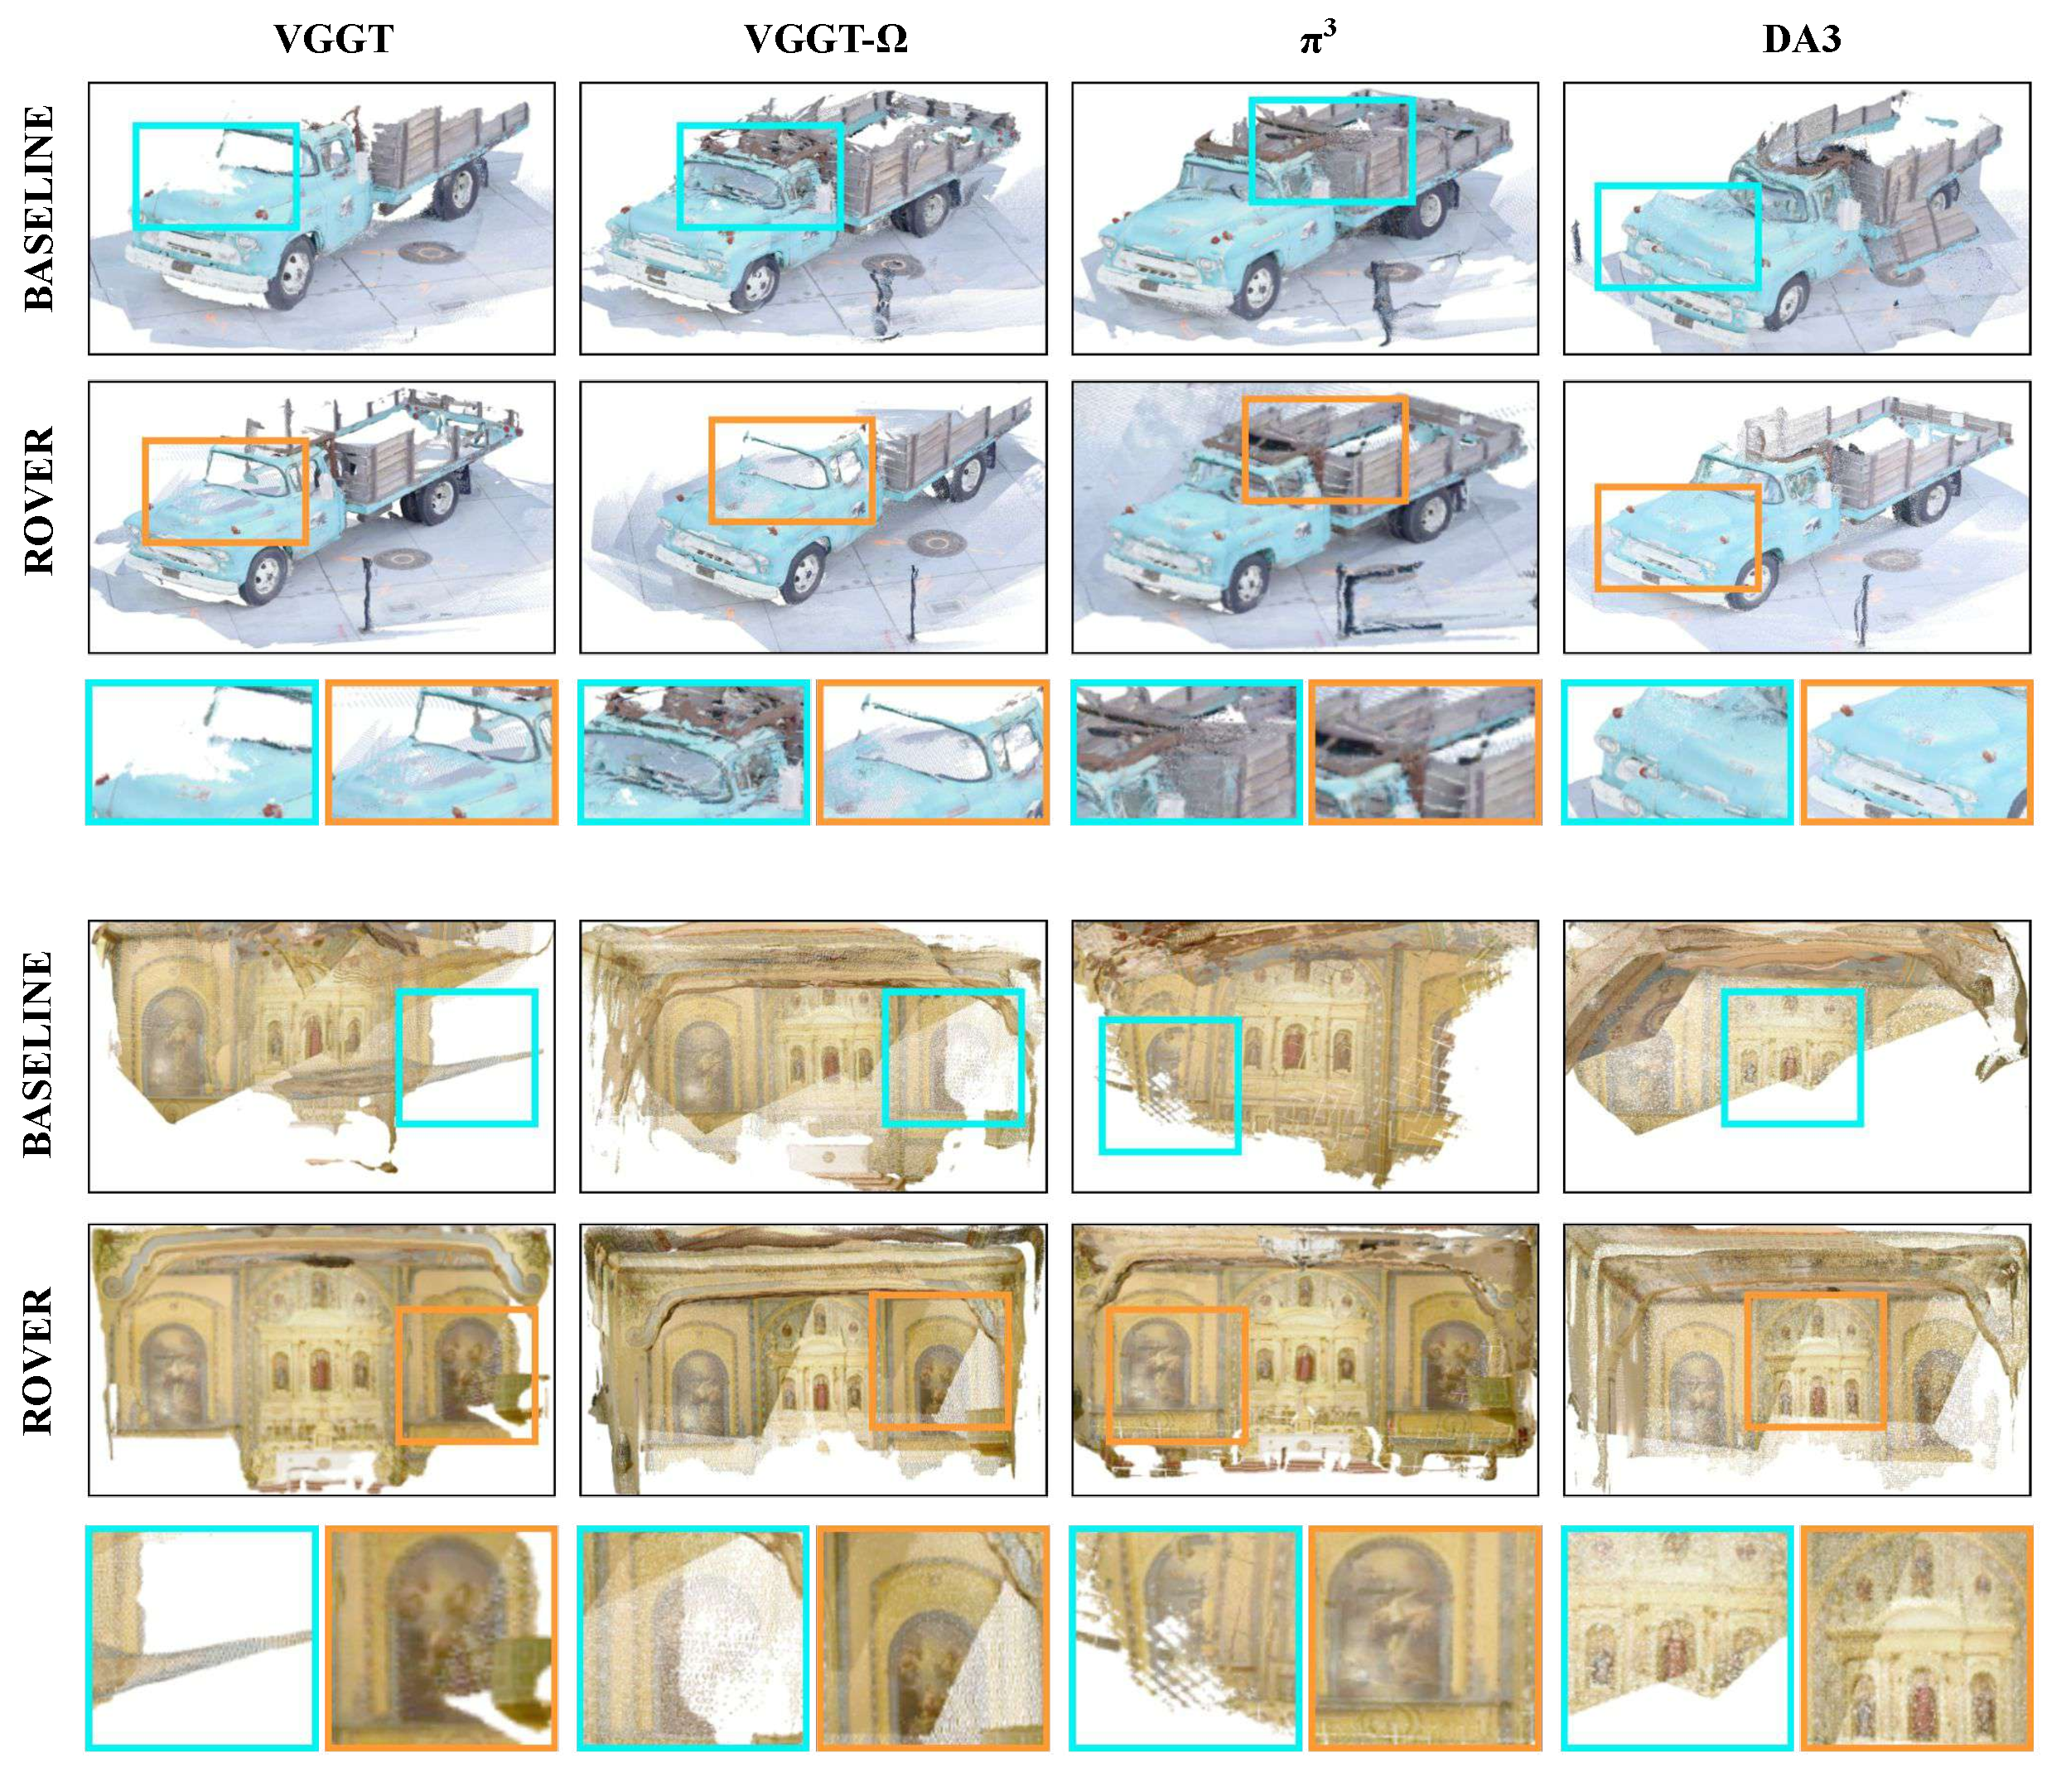
\includegraphics[width=\textwidth]{supplementary_figures/pointcloud_comparisons/supplementary_fig_1.pdf}
\caption{\textbf{Qualitative comparison on the Tanks \& Temples dataset} (Truck and Church scenes). Point cloud reconstructions across VGGT, VGGT-$\Omega$, $\pi^3$, and DA3 comparing baseline and ROVER.}
\label{fig:pc_tanks_and_temples}

\vspace{4mm}

% --- Dataset 2 (Part 1): 7-Scenes (Office) ---
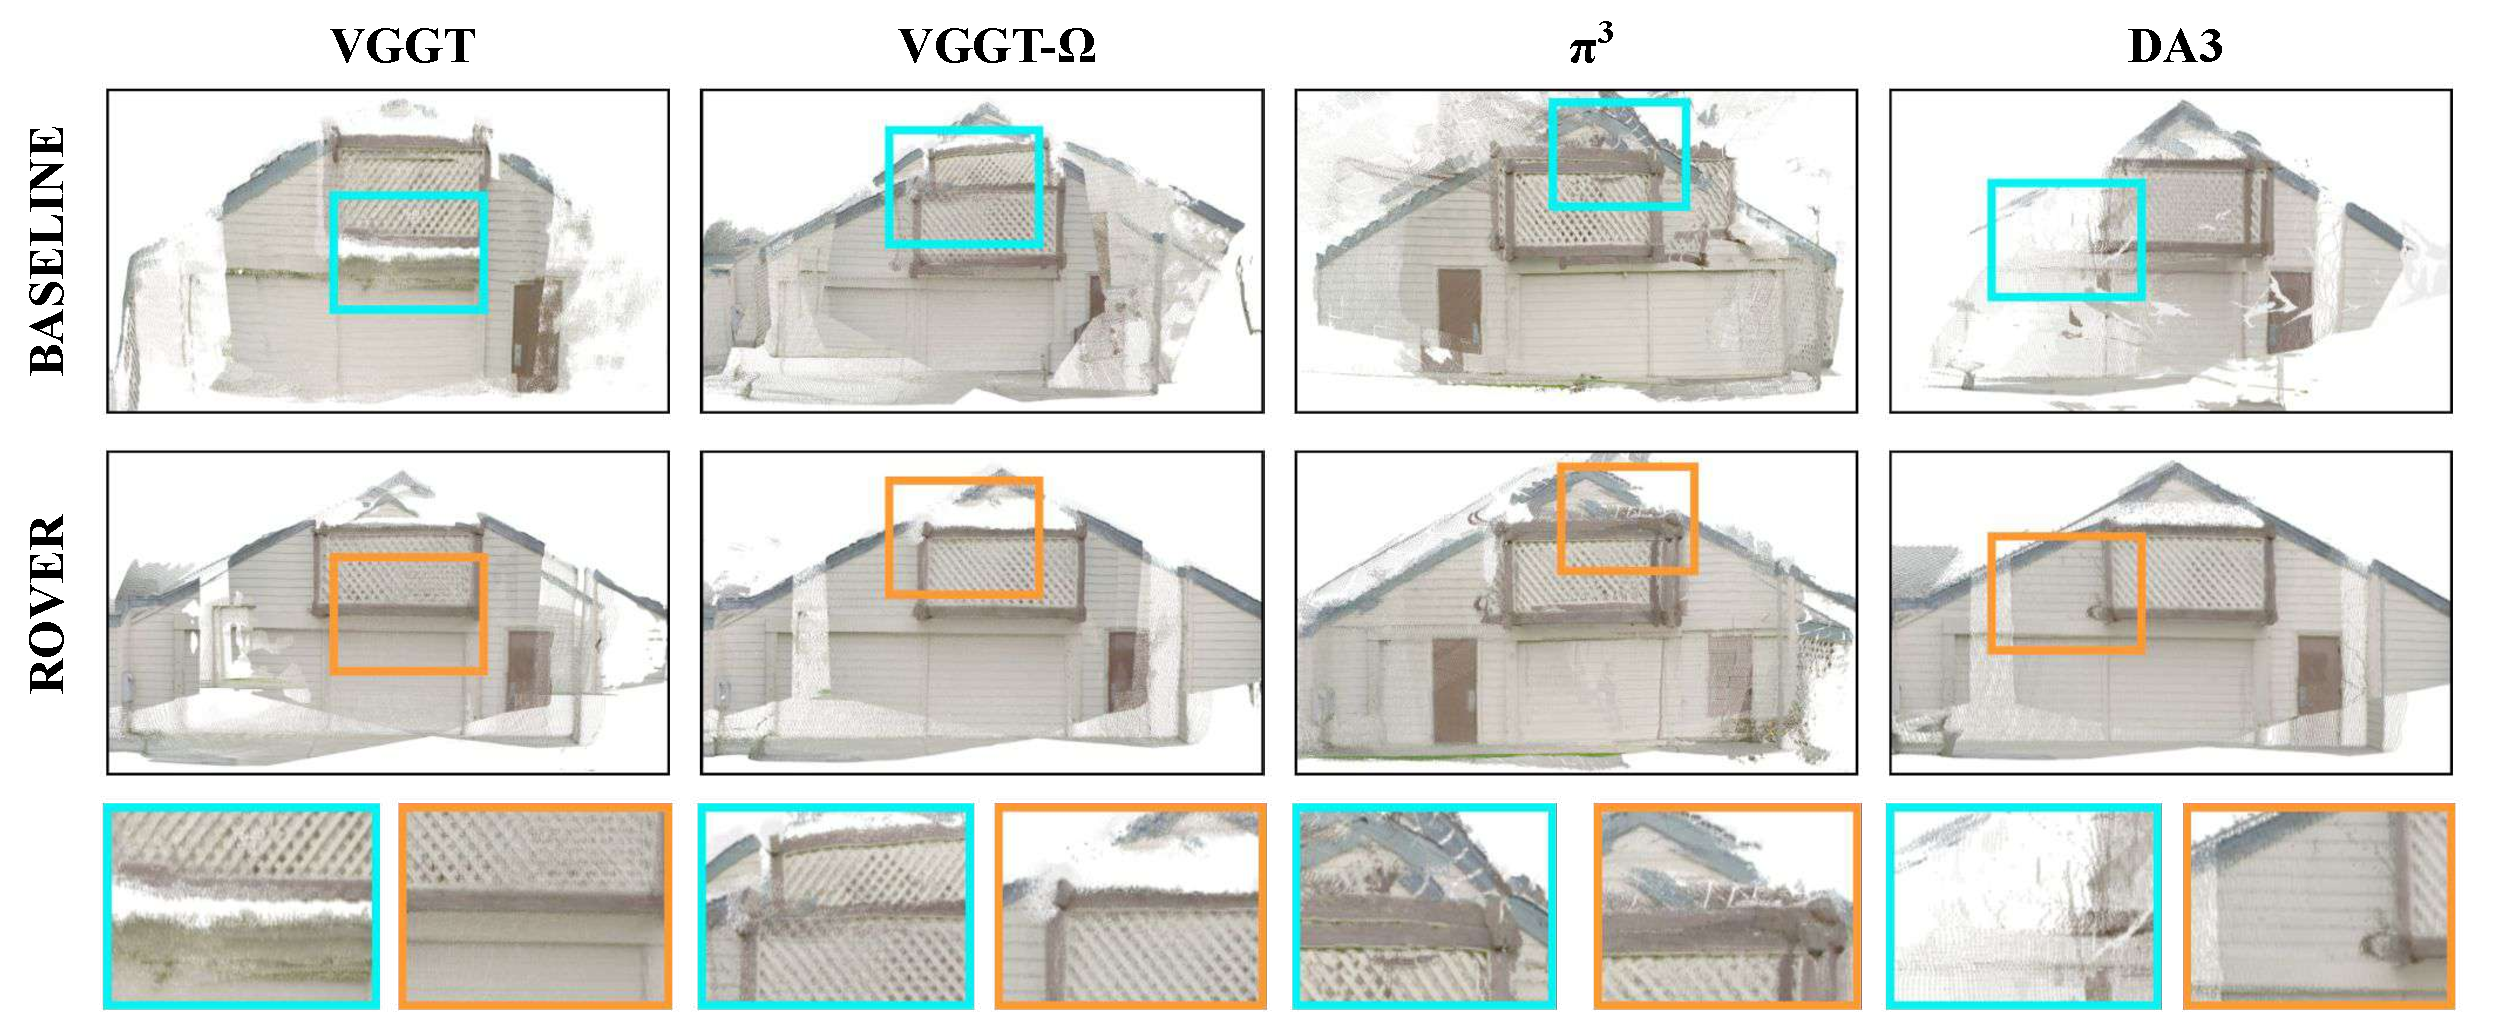
\includegraphics[width=\textwidth]{supplementary_figures/pointcloud_comparisons/supplementary_fig_2.1.pdf}
\caption{\textbf{Qualitative comparison on the Barn scene} from Tanks \& Temples dataset . Reconstruction comparisons across baseline and ROVER settings.}
\label{fig:pc_tnt_barn}

\end{figure*}


% \clearpage % Pushes the next figure onto its own new page

% =========================================================================
% PAGE 2: 7-Scenes (Kitchen)
% =========================================================================
\begin{figure*}[!t]
\centering

% --- Dataset 2 (Part 2): 7-Scenes (Kitchen) ---
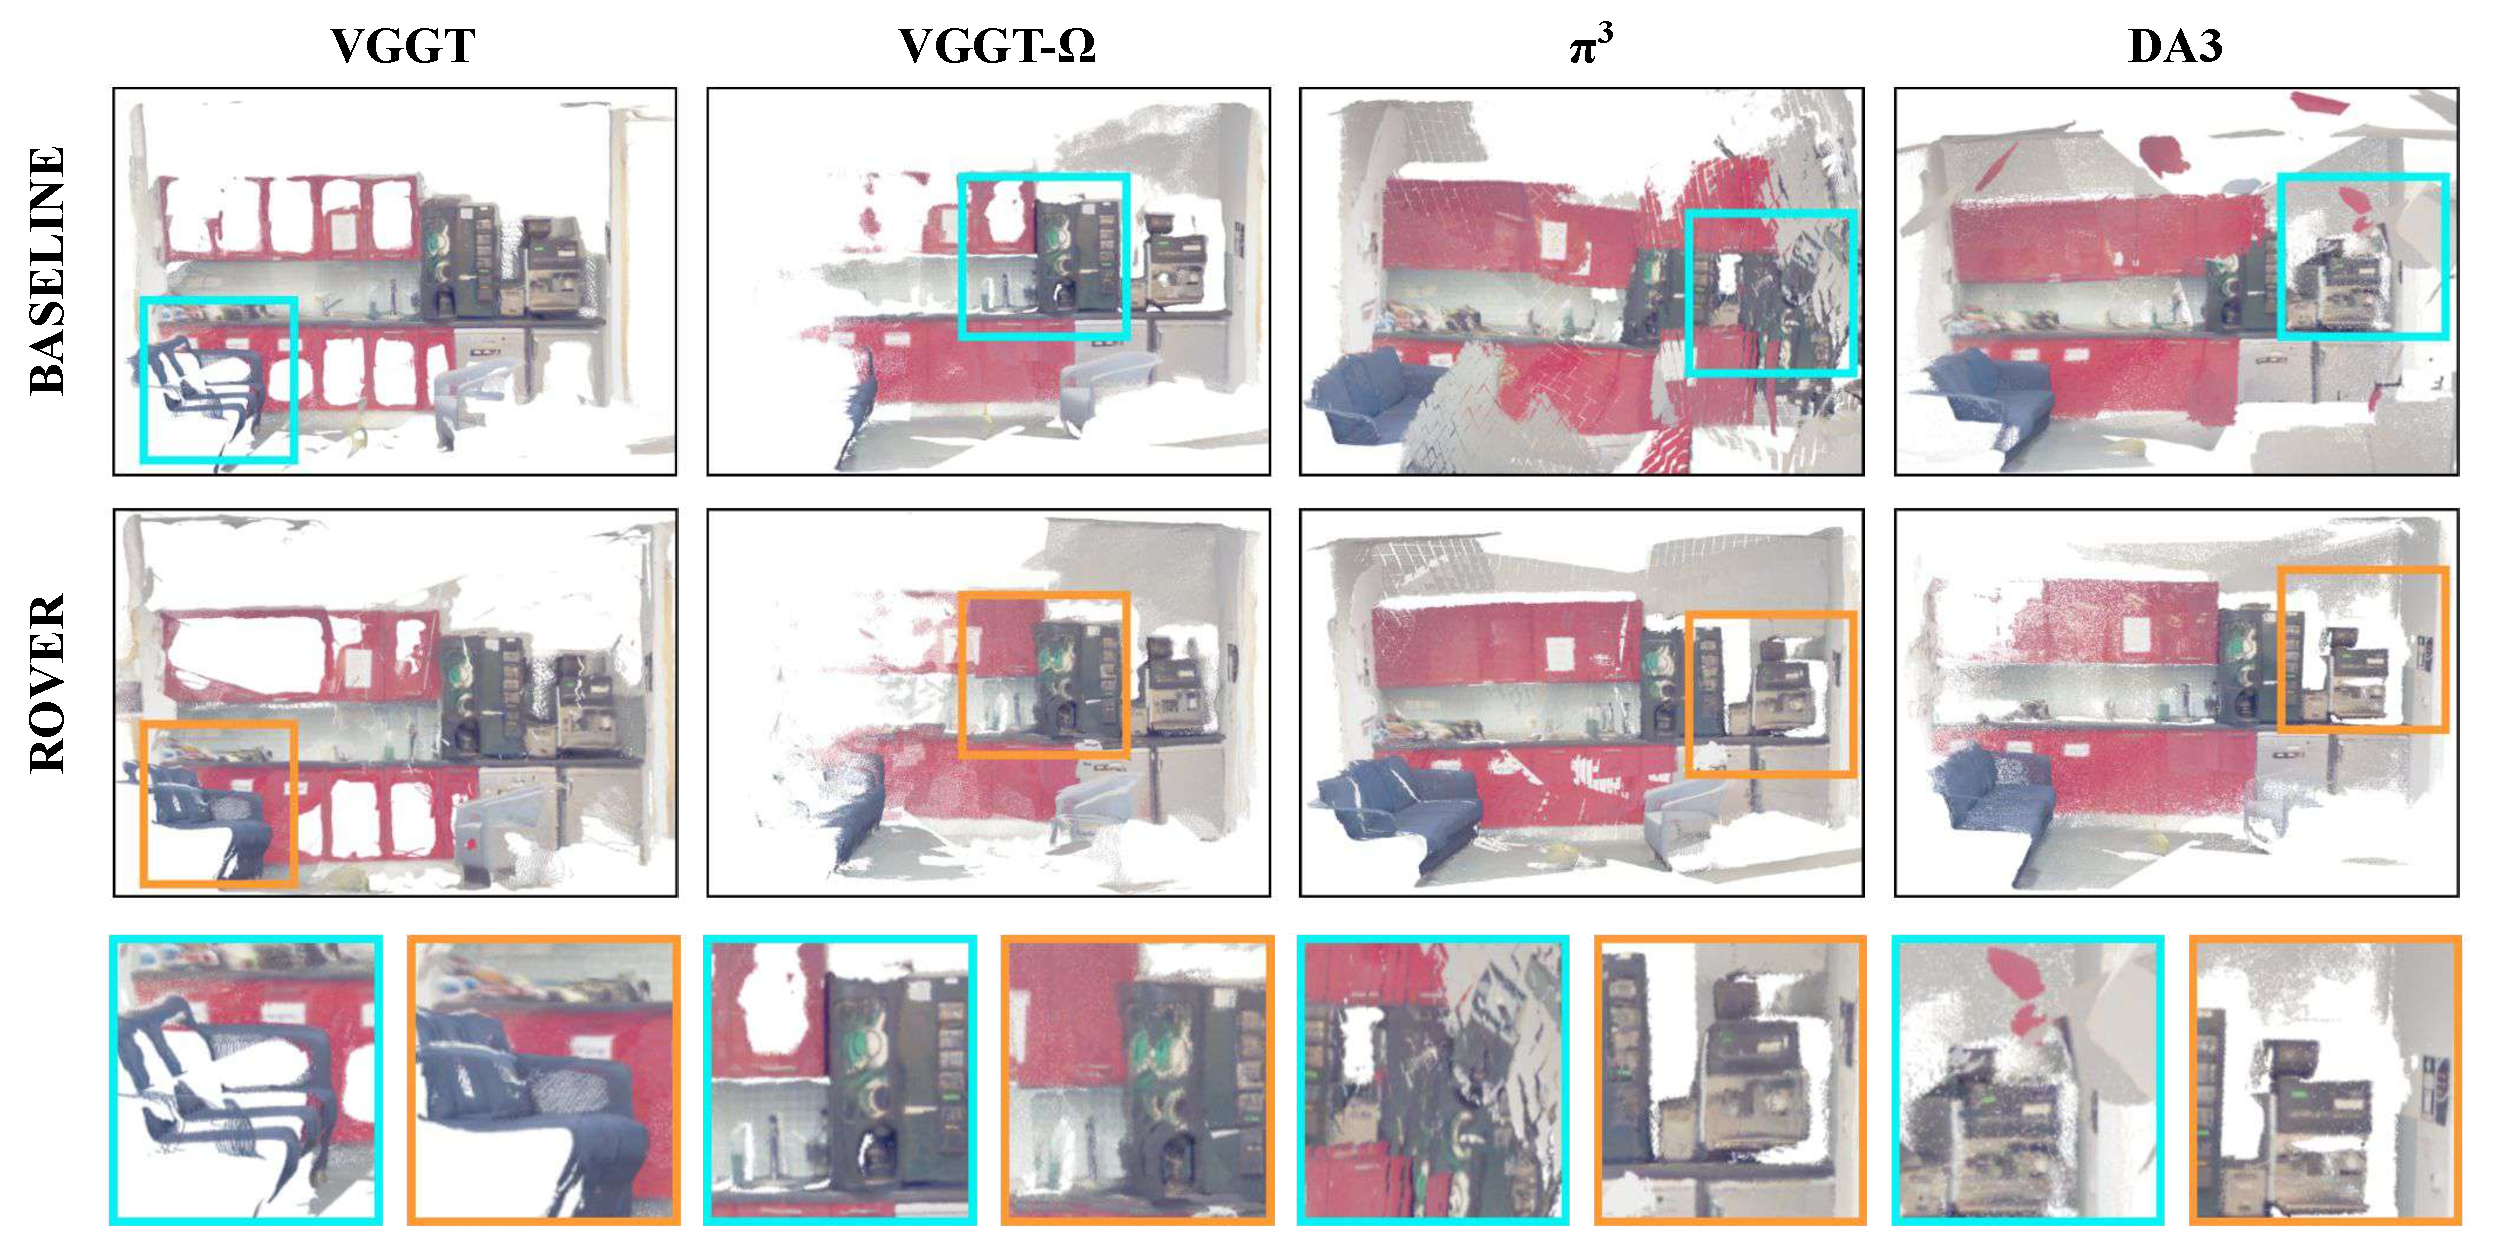
\includegraphics[width=0.97\textwidth]{supplementary_figures/pointcloud_comparisons/supplementary_fig_2.2.pdf}
\caption{\textbf{Qualitative comparison on the 7-Scenes dataset (Red Kitchen scene)}. Close-up comparisons showing geometric alignment and wall boundary recovery under ROVER.}
\label{fig:pc_7scenes_kitchen}

\end{figure*}
%%%%%%%%%%%%%%%%%%%%%%%%%%%%%%%%%%%%%%%%%%%%%%%

% \begin{figure*}[h]
% \centering
% 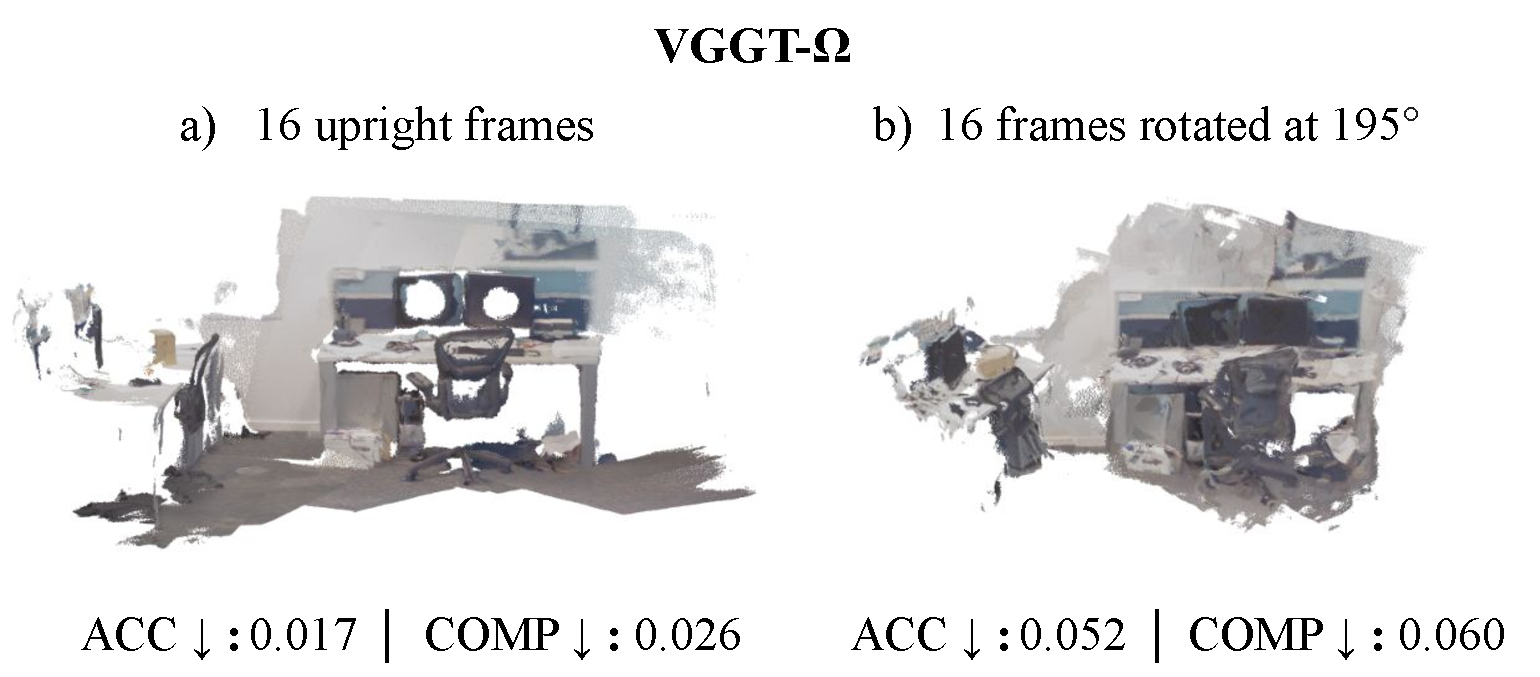
\includegraphics[width=0.86\textwidth]{Figures/pc_comparison.pdf}
% \caption{\textbf{Comparison between upright inputs (left) and inputs rotated by 195$^\circ$ (right).} The reconstructed point cloud degrades even when the same rotation is applied consistently to all input images.}
% \label{fig:all_rot}
% \end{figure*}


\begin{figure}[H]
\centering
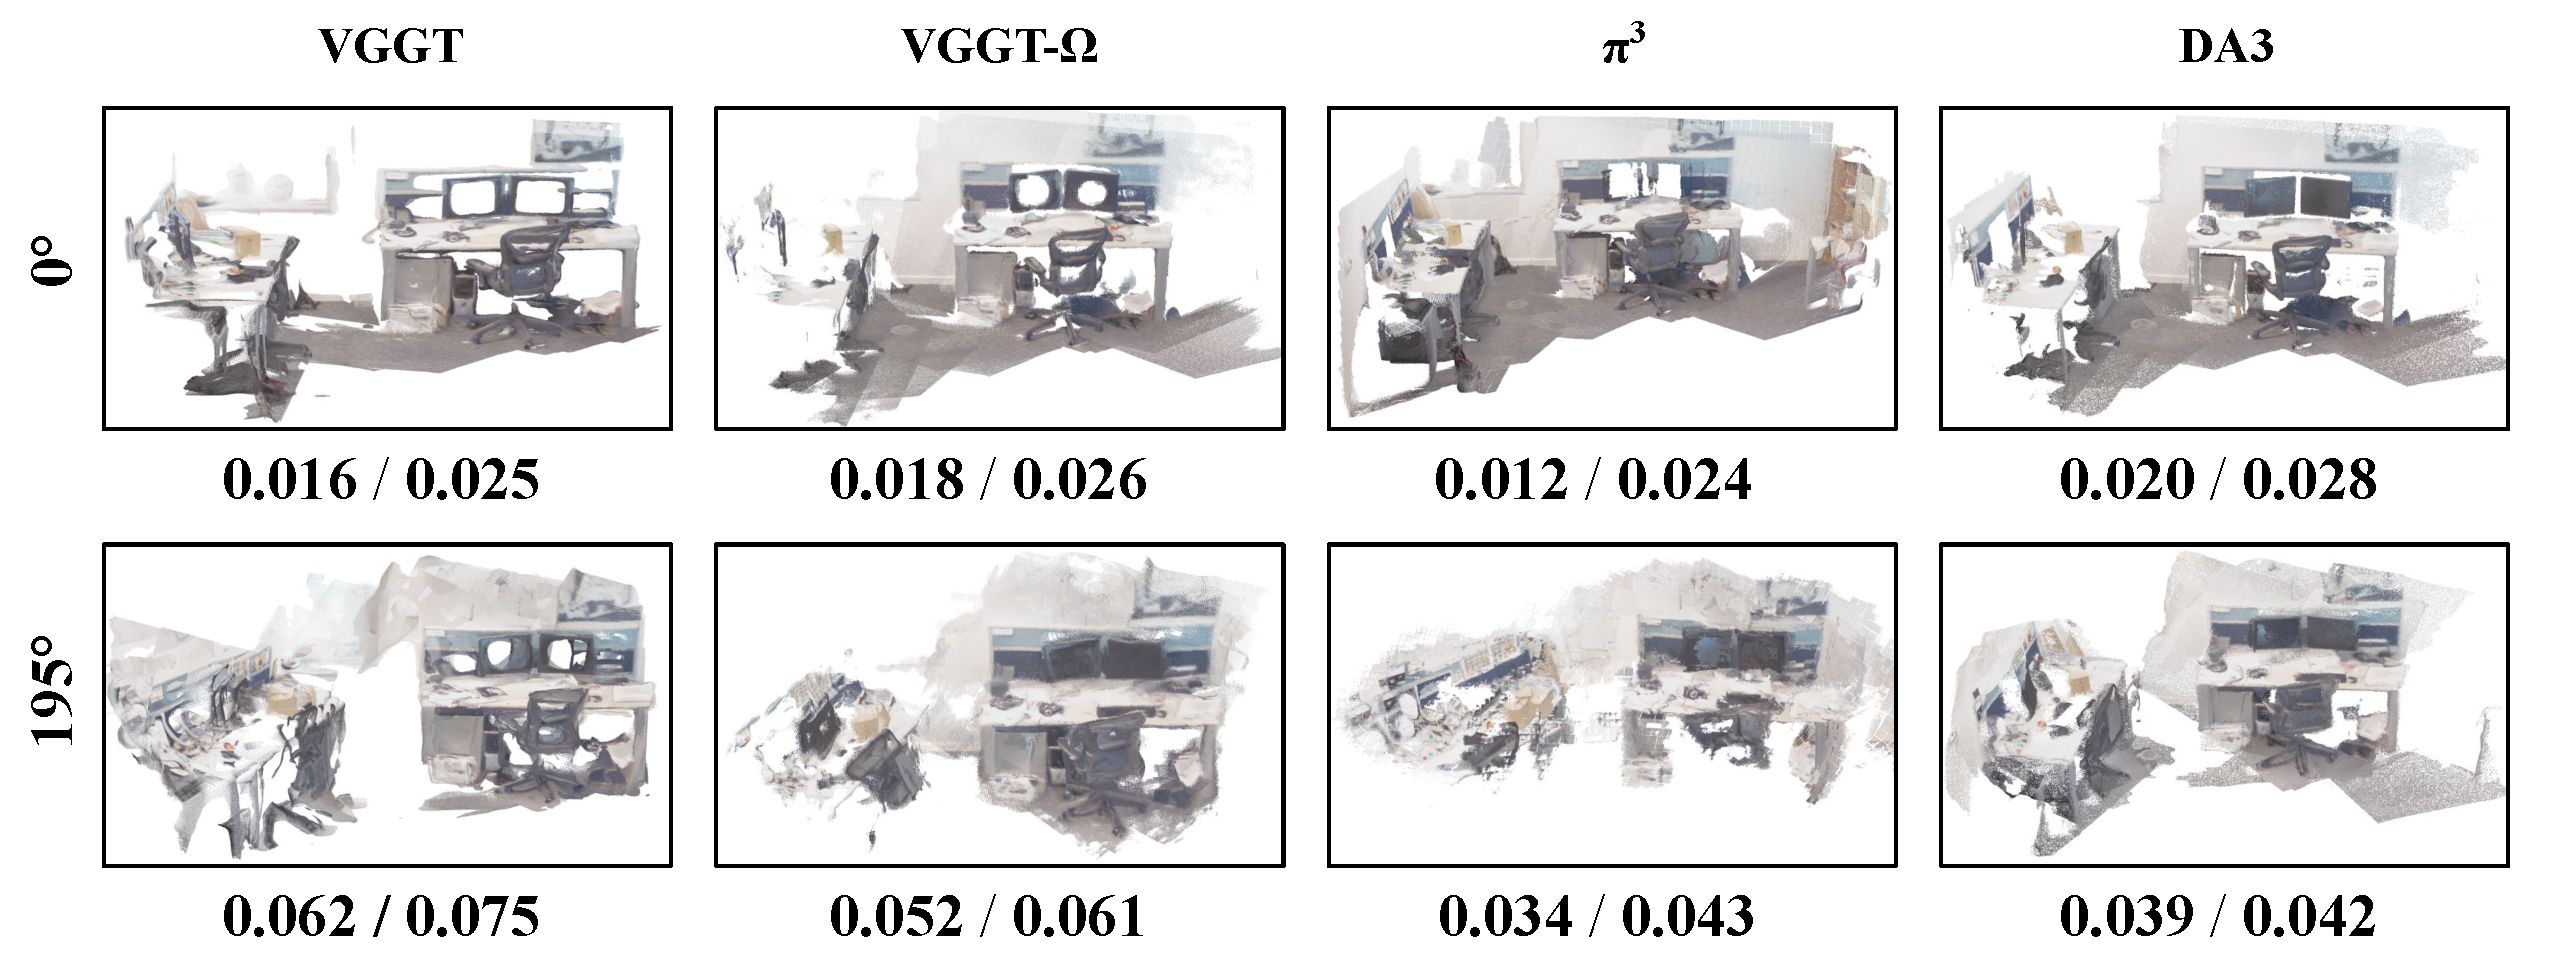
\includegraphics[width=\linewidth]{supplementary_figures/rotation_pc_comparison.pdf}
\caption{\textbf{Degradation under uniform roll on ETH3D (\emph{office}).} Point cloud reconstructions comparing clean upright views ($0^\circ$, top row) with sequences where every input view is rotated identically by $195^\circ$ (bottom row). Numbers denote Accuracy (Acc $\downarrow$) / Completeness (Comp $\downarrow$) in meters relative to ground truth . Degradation occurs despite identical relative poses between views, confirming reliance on an absolute upright prior.}
\label{fig:uniform_rotation_office}
\end{figure}

\section{Sensitivity to Yaw Rotations}
\label{sec:pose_yaw}
We additionally evaluate sensitivity to camera rotations about the yaw axis on NRGB-D, 7-Scenes, and Tanks\&Temples in~\Cref{tab:yaw_metrics}. Following the evaluation protocol described in~\Cref{sec:experimental_setup}, we evaluate the four non-zero rotation levels, with selected views independently assigned yaw perturbations from $[-20^\circ,+20^\circ]$. Large perturbation across yaw will lead to change in viewpoint of the scene which is not a manisfestation of UprightBias thus we restrict the evaluation to limited perturbation.  The corresponding camera poses are perturbed and new views are rendered using~\Cref{sec:rendering_based_rotation}. Overall, yaw perturbations introduce moderate degradation, particularly on Tanks\&Temples. For example, $\pi^3$ decreases from $0.721$ to $0.667$ N.C., while MapAnything decreases from $0.627$ to $0.592$ N.C. and from $94.53$ to $92.57$ AUC$_{30}$. 
\begin{table}[h]
\centering
\caption{Point-map (N.C., $\uparrow$) and pose (AUC$_{30}$, $\uparrow$) accuracy for upright inputs and inputs rotated about the yaw axis, on NRGBD, 7-Scenes, and Tanks\&Temples.}
\label{tab:yaw_metrics}
\small
\setlength{\tabcolsep}{3.5pt}
\resizebox{\linewidth}{!}{%
\begin{tabular}{l *{3}{cccc}}
\toprule
 & \multicolumn{4}{c}{\textbf{NRGBD}}
 & \multicolumn{4}{c}{\textbf{7-Scenes}}
 & \multicolumn{4}{c}{\textbf{Tanks\&Temples}} \\
\cmidrule(lr){2-5} \cmidrule(lr){6-9} \cmidrule(lr){10-13}

 & \multicolumn{2}{c}{N.C. $\uparrow$}
 & \multicolumn{2}{c}{AUC$_{30}$ $\uparrow$}
 & \multicolumn{2}{c}{N.C. $\uparrow$}
 & \multicolumn{2}{c}{AUC$_{30}$ $\uparrow$}
 & \multicolumn{2}{c}{N.C. $\uparrow$}
 & \multicolumn{2}{c}{AUC$_{30}$ $\uparrow$} \\
\cmidrule(lr){2-3} \cmidrule(lr){4-5}
\cmidrule(lr){6-7} \cmidrule(lr){8-9}
\cmidrule(lr){10-11} \cmidrule(lr){12-13}

\textbf{Method}
& Upright & Rotated & Upright & Rotated
& Upright & Rotated & Upright & Rotated
& Upright & Rotated & Upright & Rotated \\
\midrule

VGGT
& \dd{0.795}{0.030} & \dd{0.788}{0.010}
& \dd{98.65}{0.86} & \dd{97.59}{0.82}
& \dd{0.659}{0.033} & \dd{0.665}{0.006}
& \dd{85.80}{9.53} & \dd{84.44}{2.25}
& \dd{0.685}{0.042} & \dd{0.659}{0.032}
& \dd{94.18}{9.62} & \dd{93.33}{1.63} \\
\addlinespace[3pt]

VGGT-$\Omega$
& \dd{0.825}{0.048} & \dd{0.825}{0.008}
& \dd{99.10}{0.72} & \dd{98.46}{0.63}
& \dd{0.672}{0.040} & \dd{0.679}{0.006}
& \dd{89.35}{5.07} & \dd{87.78}{1.58}
& \dd{0.669}{0.080} & \dd{0.657}{0.023}
& \dd{93.27}{13.12} & \dd{93.52}{0.99} \\
\addlinespace[3pt]

$\pi^3$
& \dd{0.817}{0.066} & \dd{0.808}{0.011}
& \dd{96.17}{2.97} & \dd{95.42}{0.82}
& \dd{0.674}{0.041} & \dd{0.685}{0.008}
& \dd{87.54}{6.31} & \dd{85.94}{1.74}
& \dd{0.721}{0.059} & \dd{0.667}{0.040}
& \dd{97.76}{0.63} & \dd{97.17}{1.30} \\
\addlinespace[3pt]

MapA.
& \dd{0.739}{0.057} & \dd{0.716}{0.017}
& \dd{93.11}{5.13} & \dd{91.59}{1.54}
& \dd{0.623}{0.046} & \dd{0.636}{0.013}
& \dd{76.26}{12.07} & \dd{73.28}{3.17}
& \dd{0.627}{0.052} & \dd{0.592}{0.033}
& \dd{94.53}{0.98} & \dd{92.57}{1.79} \\
\addlinespace[3pt]

DA3
& \dd{0.819}{0.037} & \dd{0.808}{0.014}
& \dd{99.75}{0.38} & \dd{99.53}{0.25}
& \dd{0.676}{0.032} & \dd{0.684}{0.007}
& \dd{88.10}{7.73} & \dd{88.55}{1.48}
& \dd{0.674}{0.051} & \dd{0.661}{0.030}
& \dd{98.58}{2.11} & \dd{98.74}{1.36} \\

\bottomrule
\end{tabular}%
}
\end{table}

\section{The RotMV Dataset}
  \label{sec:rotmv_dataset}
  
  As discussed in \cref{sec:method}, existing multi-view datasets consist predominantly of clean, upright images. Consequently, evaluations on these datasets are
  performed by introducing synthetic camera roll using the controlled rotation synthesis described in \cref{sec:rendering_based_rotation}
  (\cref{alg:rotation_generation}). We present a novel benchmark consisting of seven real-world scenes (\textit{chairs}, \textit{foosball-table}, \textit{building},
  \textit{rooftop}, \textit{room}, \textit{statue}, and \textit{table-tennis}). We capture each scene using a camera ($4.84\,\text{mm}$, $f/1.8$, $12\,\text{MP}$,
  $4096\times3072$ resolution). Each scene is imaged from $16$ fixed viewpoints, and at each viewpoint, the camera is rolled in-plane through $12$ orientations
  spanning a full $360^\circ$ (in $30^\circ$ increments), resulting in $192$ images per scene.
 
  For each viewpoint, we estimate the base camera pose from the upright ($0^\circ$) image using VGGT~\citep{wang2025vggt}. The poses corresponding to the remaining $11$
  roll angles are then derived from this base pose by applying the corresponding in-plane rotation to the camera orientation, while keeping the camera center and viewing
  direction unchanged. Thus, pose estimation is performed only for the upright image at each viewpoint, and the poses for the other roll angles are constructed
  analytically. This enables a robust evaluation of each method under realistic in-plane camera roll, while keeping the underlying scene geometry and viewpoint fixed.

  We show example images from our dataset in Figures \Cref{fig:grid_foosball} and \Cref{fig:grids_chairs_rooftop}.


% =========================================================================
% PAGE 1: Foosball Table (Bottom of Page G-5)
% =========================================================================
\begin{figure}[!htb]
\centering
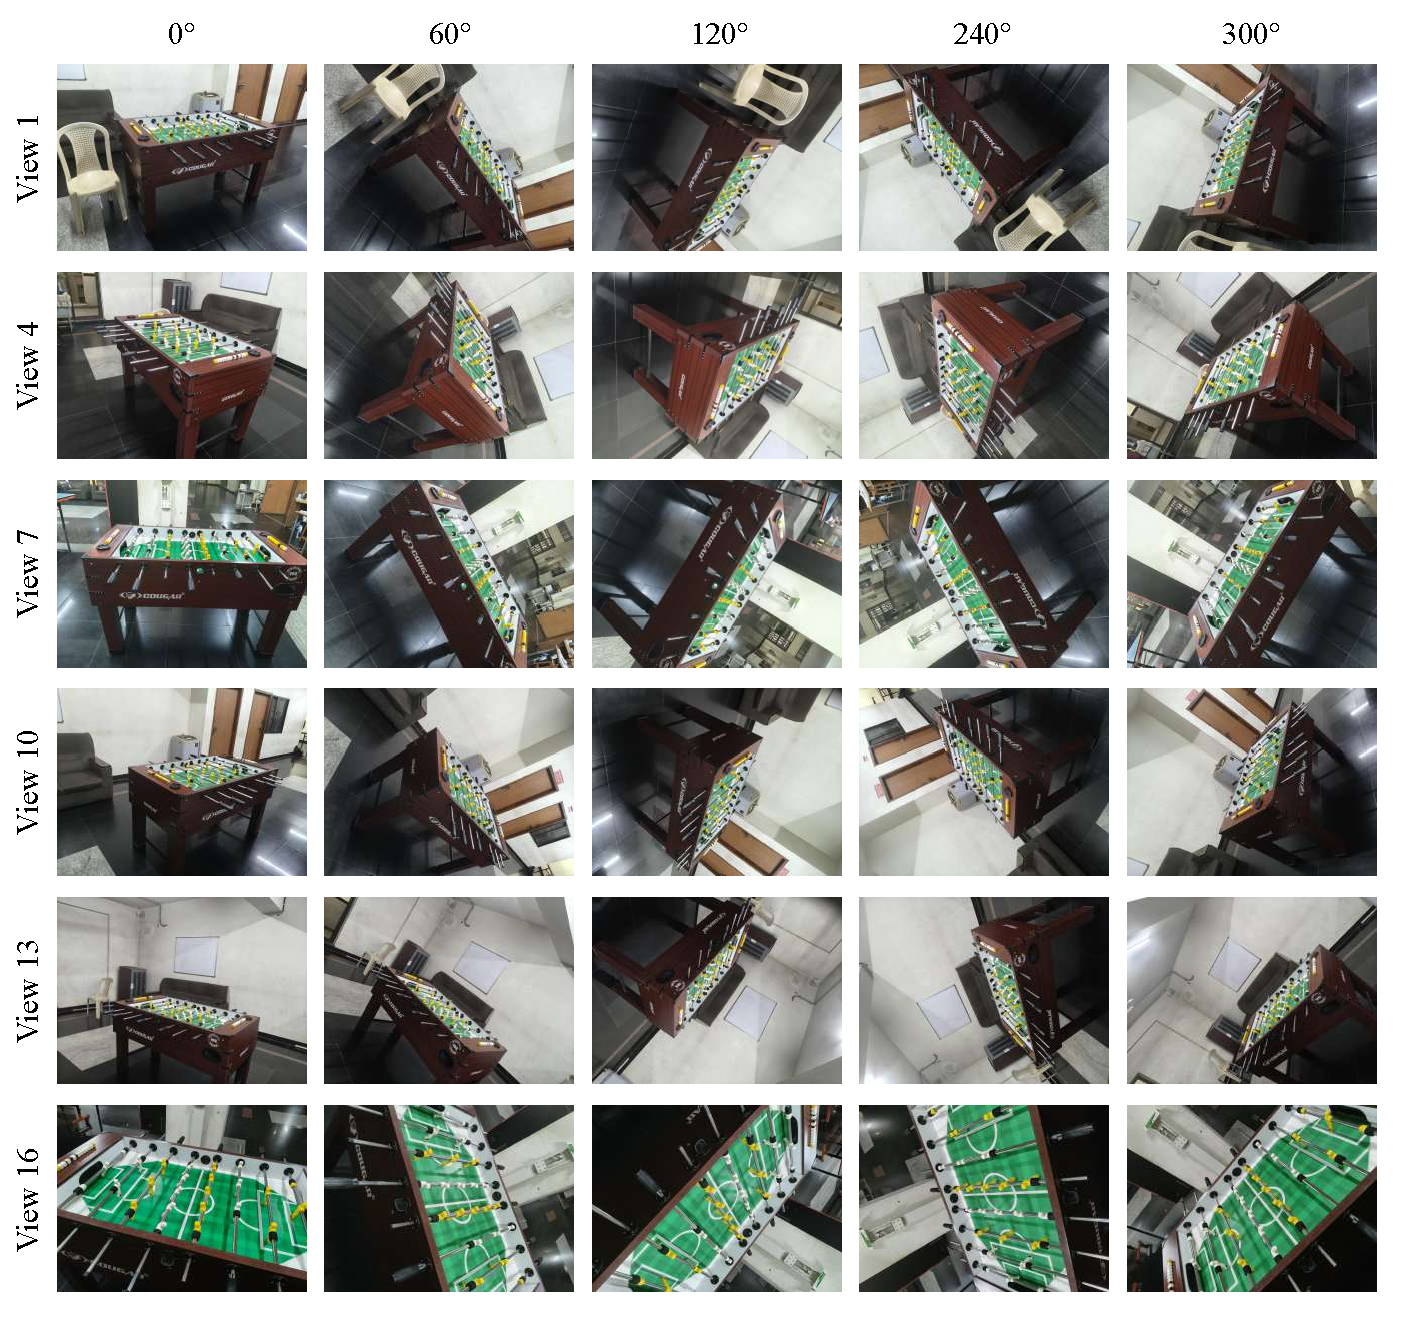
\includegraphics[
    height=0.55\textheight,
    keepaspectratio
]{Figures/captured_supplementary/foosball_compressed.pdf}
\vspace{1mm}
\caption{\textbf{RotMV dataset roll sweeps: Foosball Table (Indoor).}
Sampled views (rows) across in-plane roll angles
($\theta \in [0^\circ, 300^\circ]$, columns).}
\label{fig:grid_foosball}
\end{figure}

% \clearpage

% =========================================================================
% PAGE 2: Chairs & Rooftop
% =========================================================================
\begin{figure}[tbp]
\centering
\vspace*{-6mm}

\begin{subfigure}[tbp]{\textwidth}
    \centering
    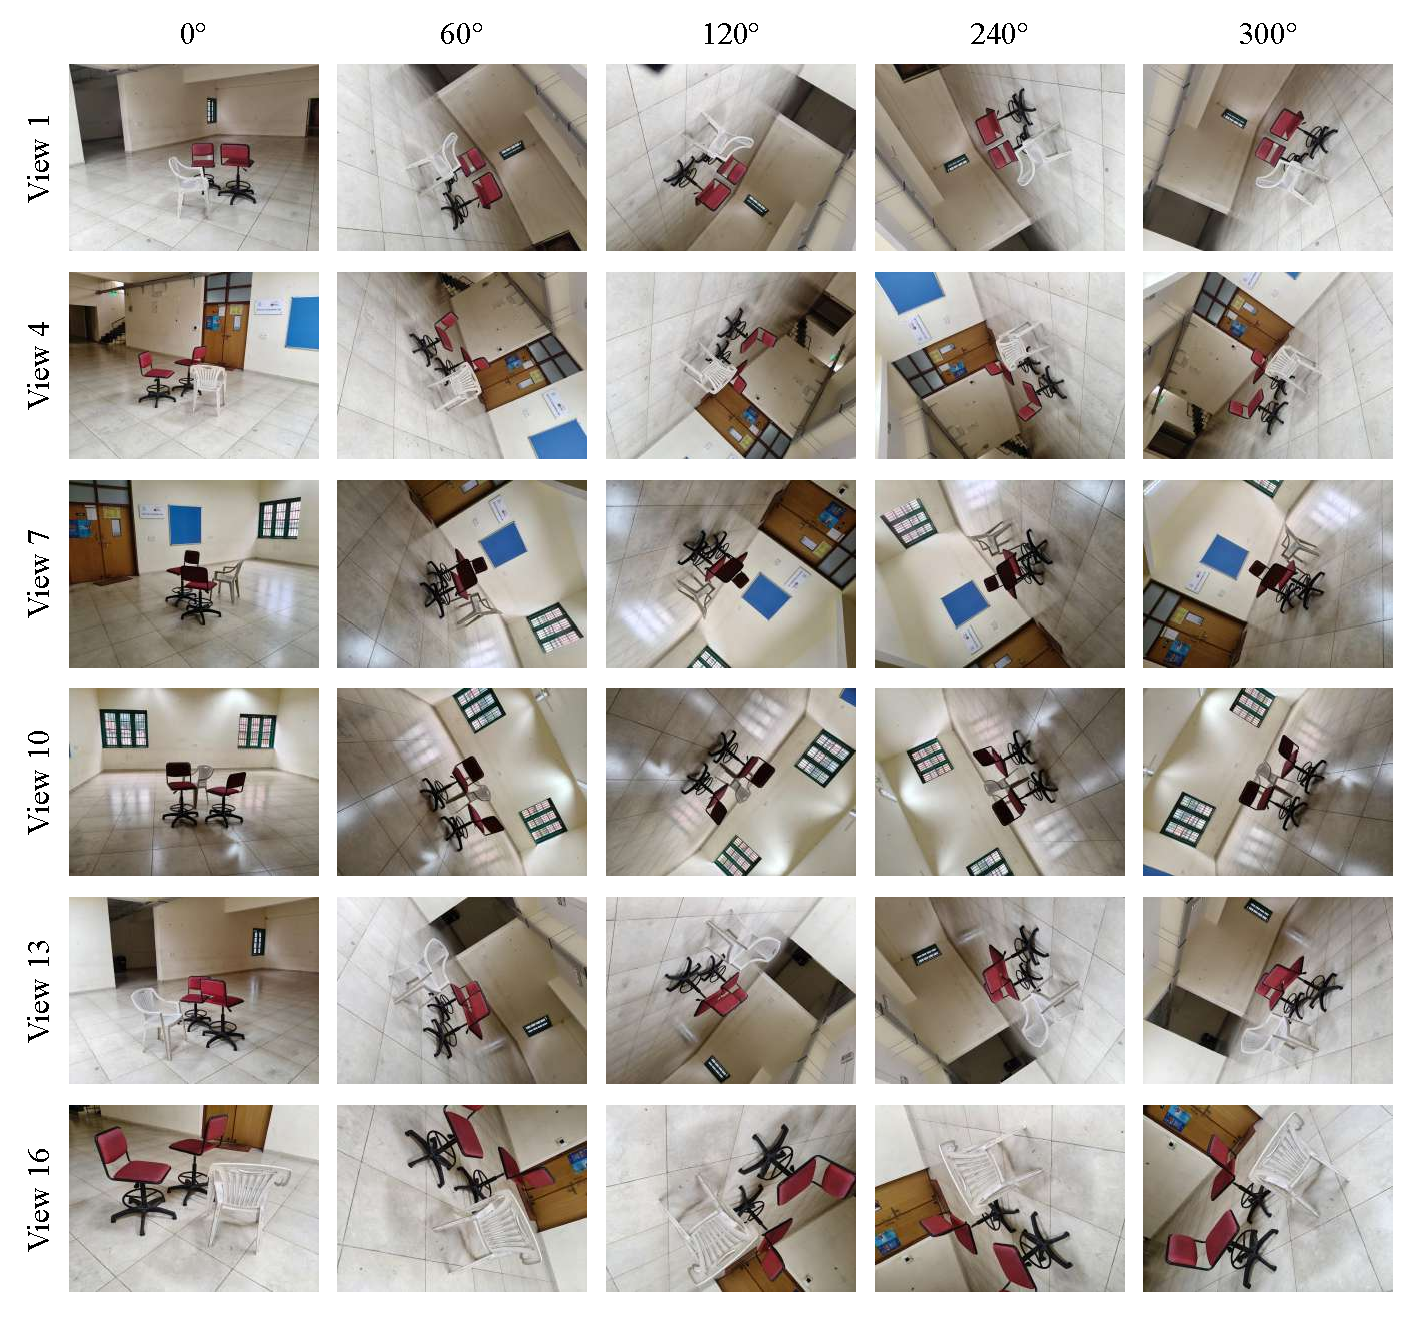
\includegraphics[
        height=0.45\textheight,
        keepaspectratio
    ]{Figures/captured_supplementary/chairs_compressed.pdf}
    \caption{Chairs (Indoor)}
    \label{fig:grid_chairs}
\end{subfigure}

\vspace{2mm}

\begin{subfigure}[tbp]{\textwidth}
    \centering
    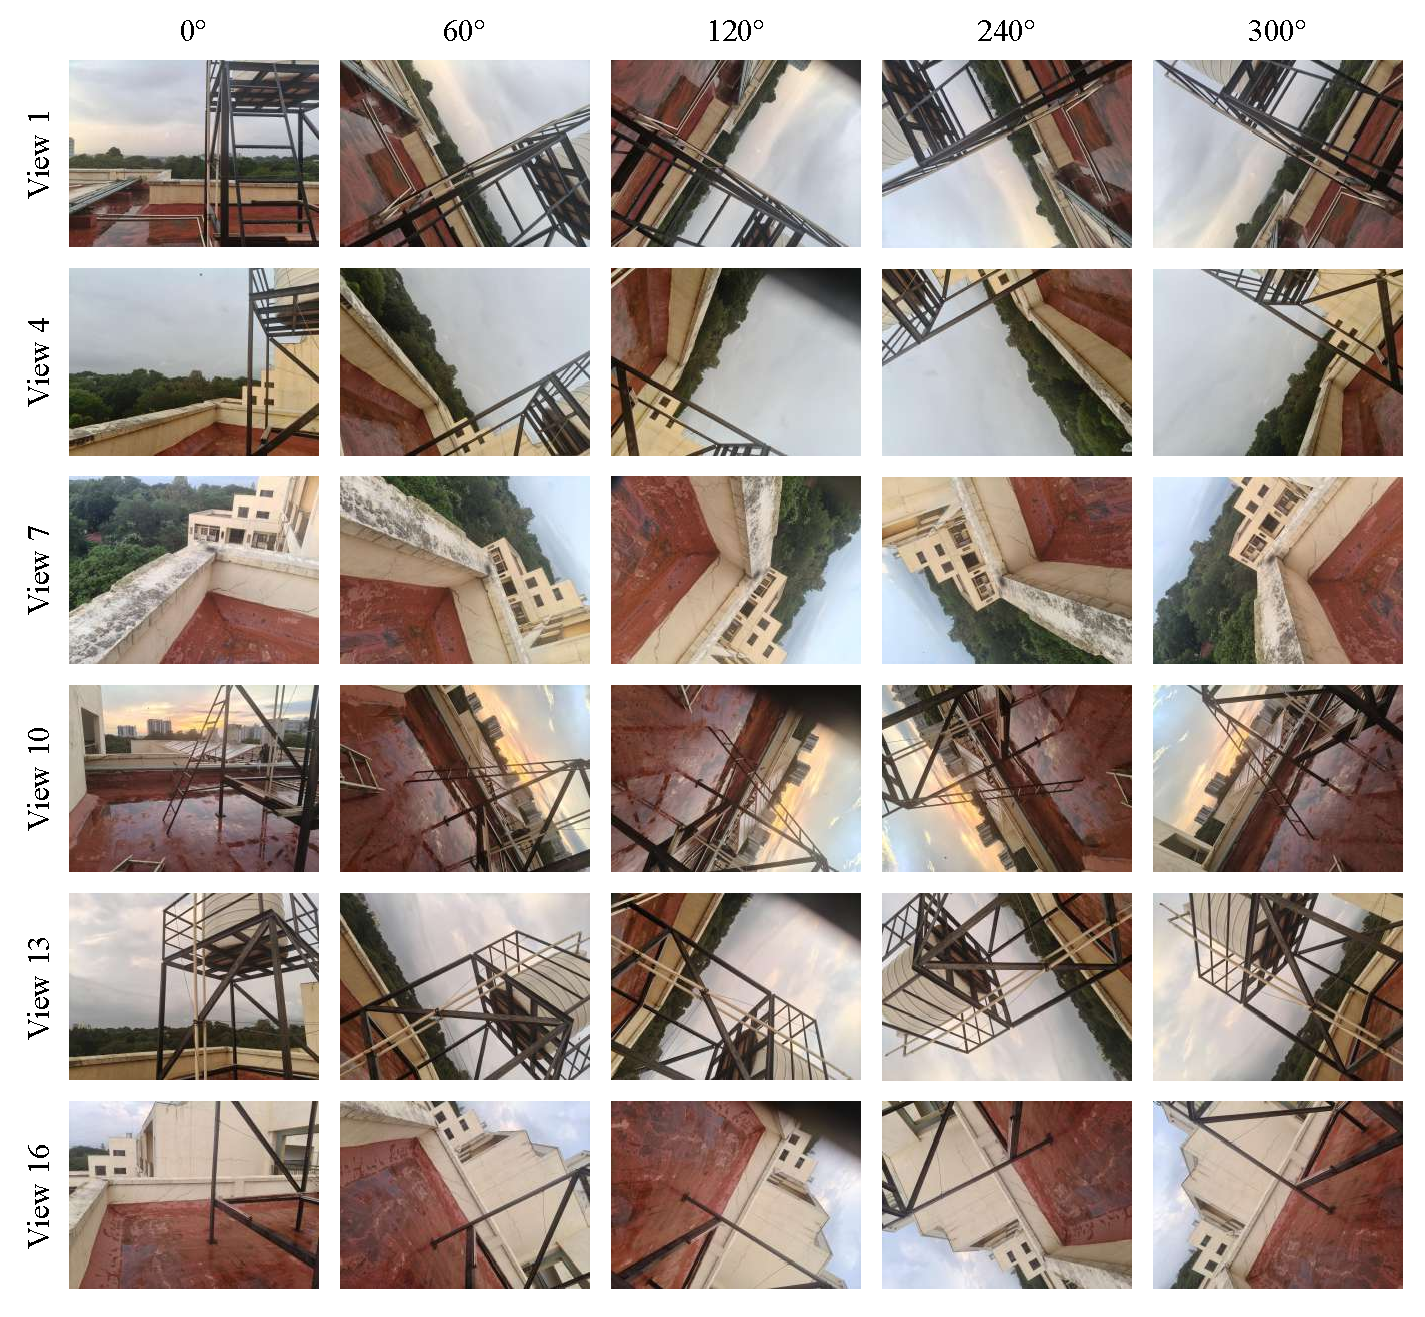
\includegraphics[
        height=0.45\textheight,
        keepaspectratio
    ]{Figures/captured_supplementary/rooftop_compressed.pdf}
    \caption{Rooftop (Outdoor)}
    \label{fig:grid_rooftop}
\end{subfigure}

\vspace{1mm}
\caption{\textbf{RotMV dataset roll sweeps: Chairs and Rooftop.}
Sampled views (rows) across in-plane roll angles
($\theta \in [0^\circ, 300^\circ]$, columns).}
\label{fig:grids_chairs_rooftop}
\end{figure}

% \clearpage
% \clearpage
% % =========================================================================
% % PAGE 1: Indoor Scenes (Foosball Table & Chairs)
% % =========================================================================
% \begin{figure*}[p]
% \centering
% \vspace*{-6mm} % Offsets float centering to utilize top margin

% % --- Top Grid: Foosball Table ---
% \begin{subfigure}[b]{\textwidth}
%   \centering
%   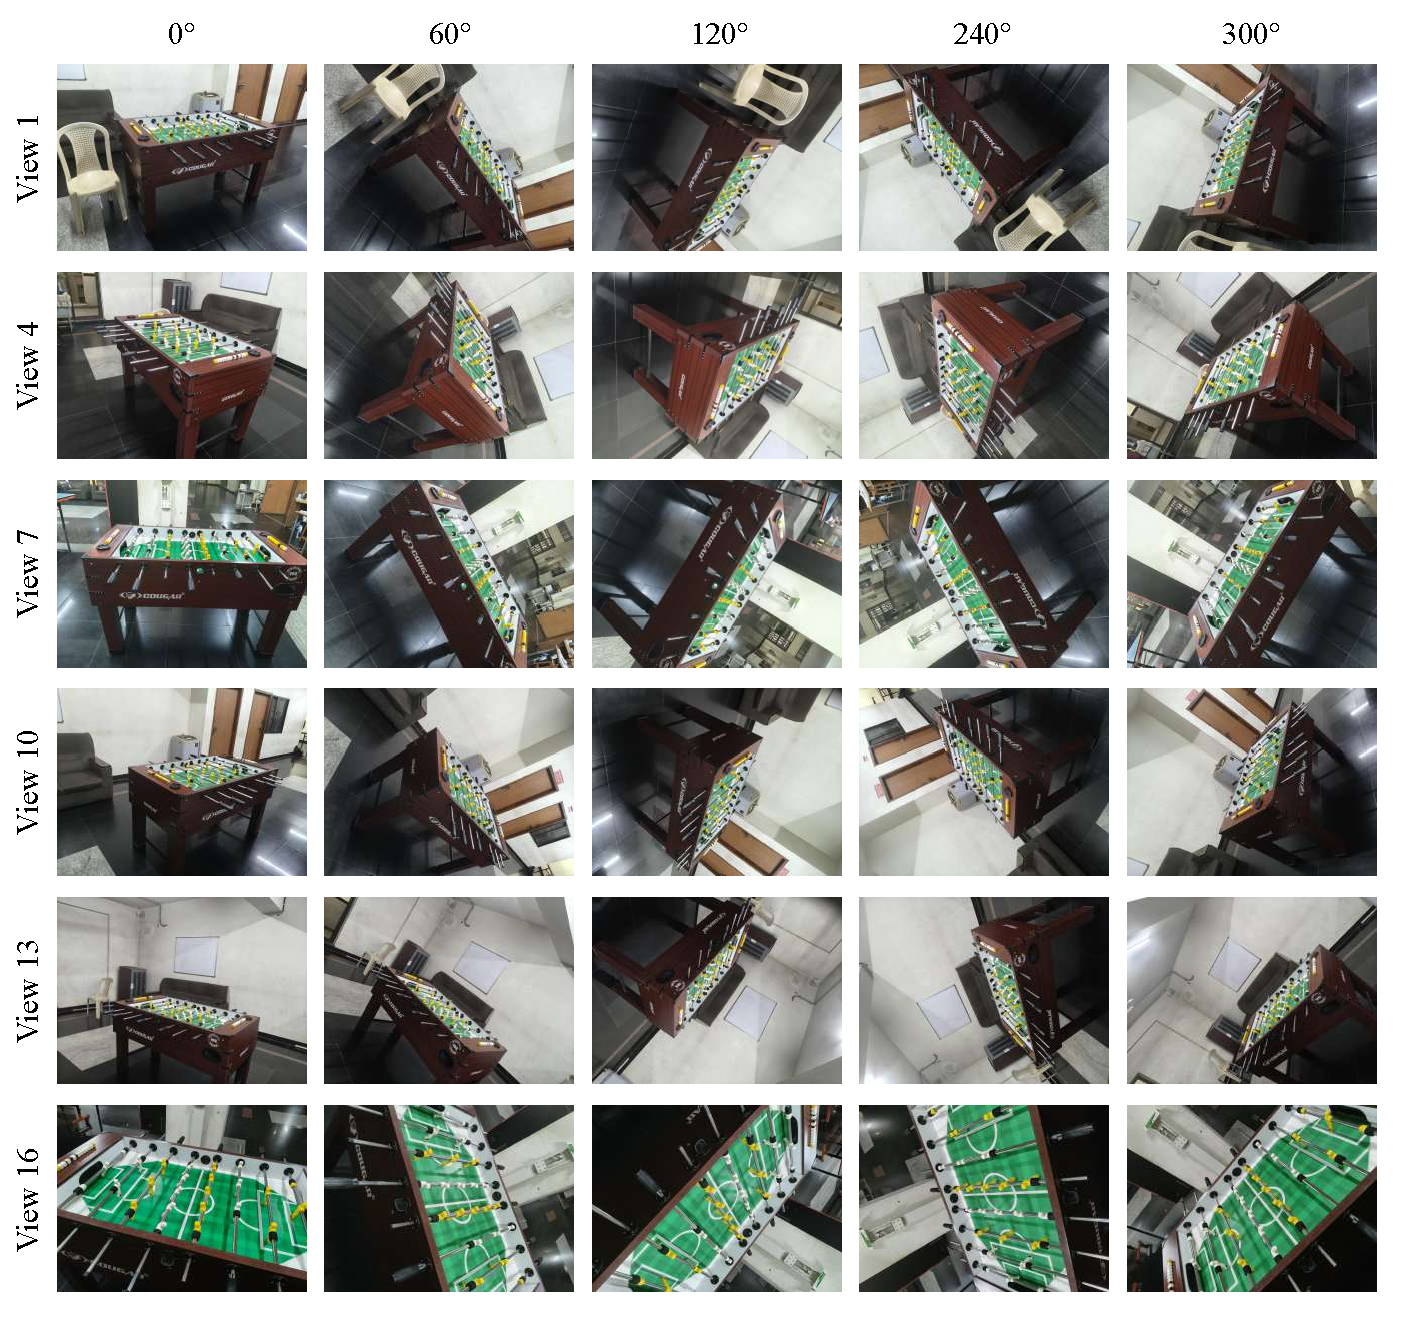
\includegraphics[height=0.47\textheight,keepaspectratio]{Figures/captured_supplementary/foosball_compressed.pdf}
%   \caption{Foosball Table}
%   \label{fig:grid_foosball}
% \end{subfigure}

% \vspace{2mm}

% % --- Bottom Grid: Chairs ---
% \begin{subfigure}[b]{\textwidth}
%   \centering
%   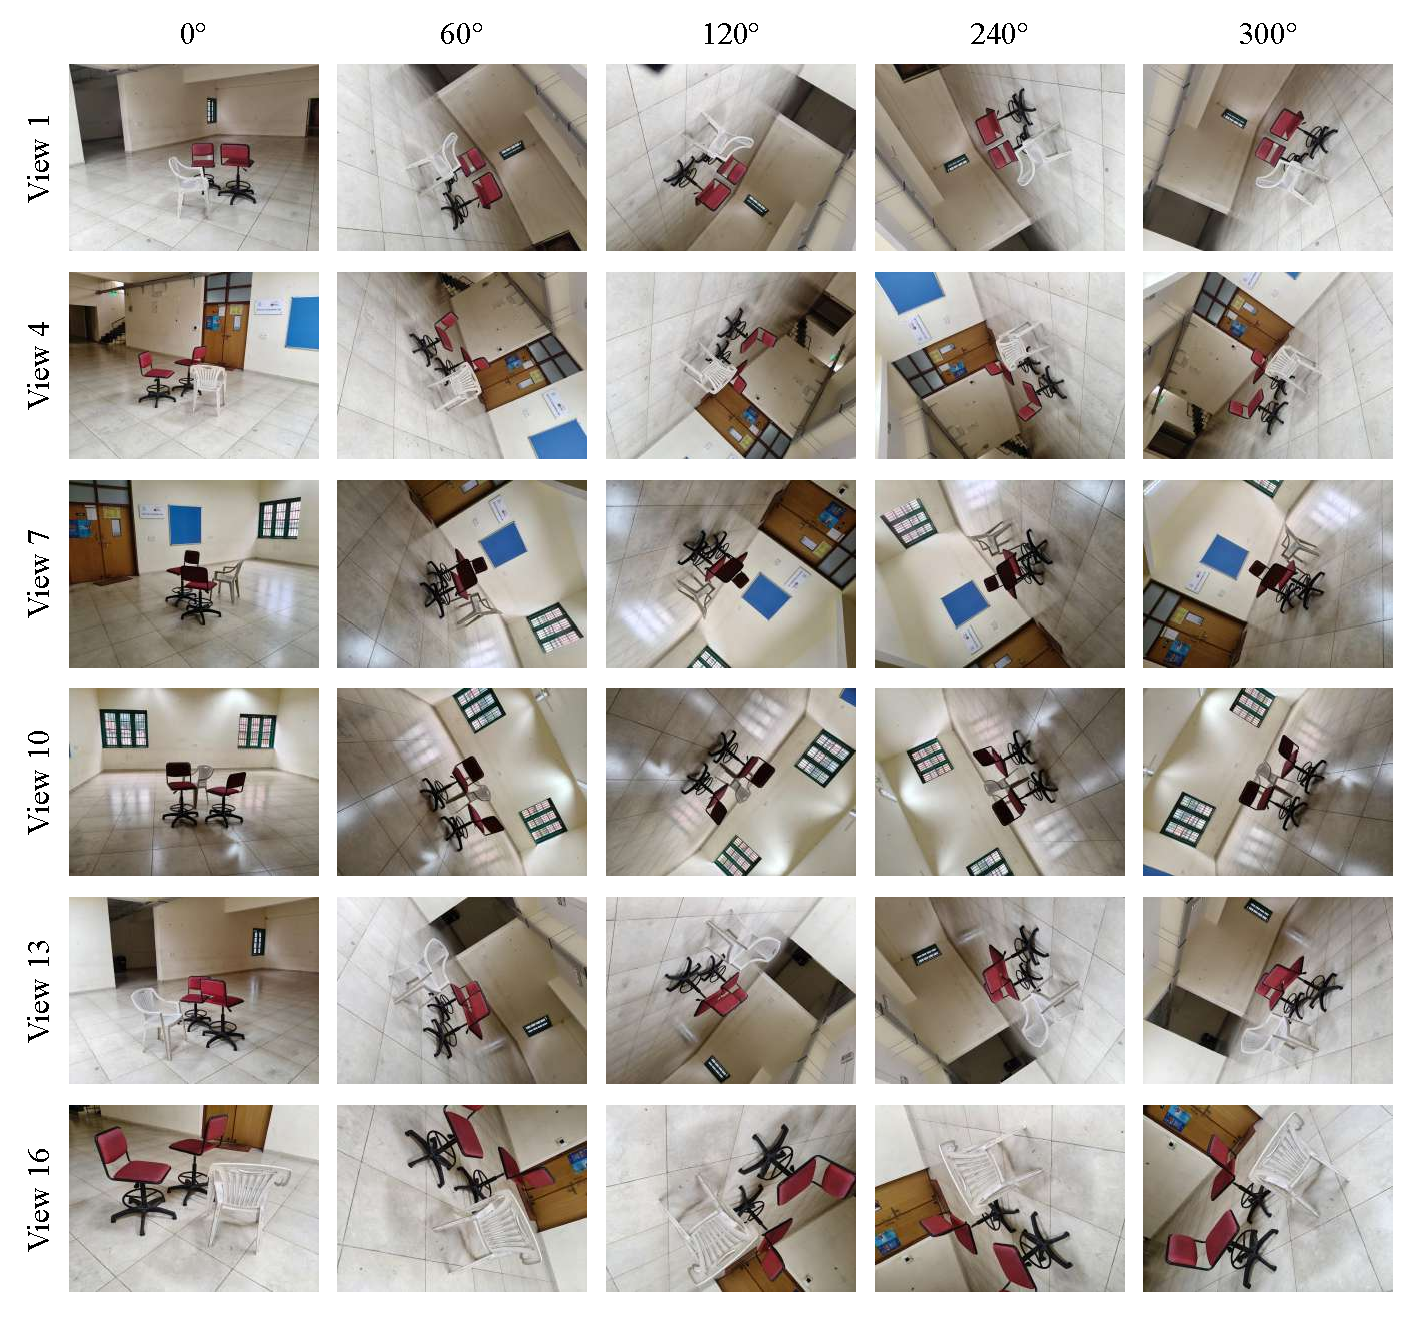
\includegraphics[height=0.48\textheight,keepaspectratio]{Figures/captured_supplementary/chairs_compressed.pdf}
%   \caption{Chairs}
%   \label{fig:grid_chairs}
% \end{subfigure}

% \vspace{1mm}
% \caption{\textbf{ROTMV dataset roll sweeps (Indoor).} Sampled views (rows) across in-plane roll angles ($0^\circ$- $300^\circ$, columns).}
% \label{fig:grids_indoor}
% \end{figure*}


% \clearpage
% % =========================================================================
% % PAGE 2: Outdoor Scenes (Building & Rooftop)
% % =========================================================================
% \begin{figure*}[p]
% \centering
% \vspace*{-6mm} % Offsets float centering to utilize top margin

% % --- Top Grid: Building ---
% % \begin{subfigure}[b]{\textwidth}
% %   \centering
% %   \includegraphics[height=0.47\textheight,keepaspectratio]{Figures/captured_supplementary/building_compressed.pdf}
% %   \caption{Building}
% %   \label{fig:grid_building}
% % \end{subfigure}

% \vspace{-4mm}

% % --- Bottom Grid: Rooftop ---
% \begin{subfigure}[b]{\textwidth}
%   \centering
%   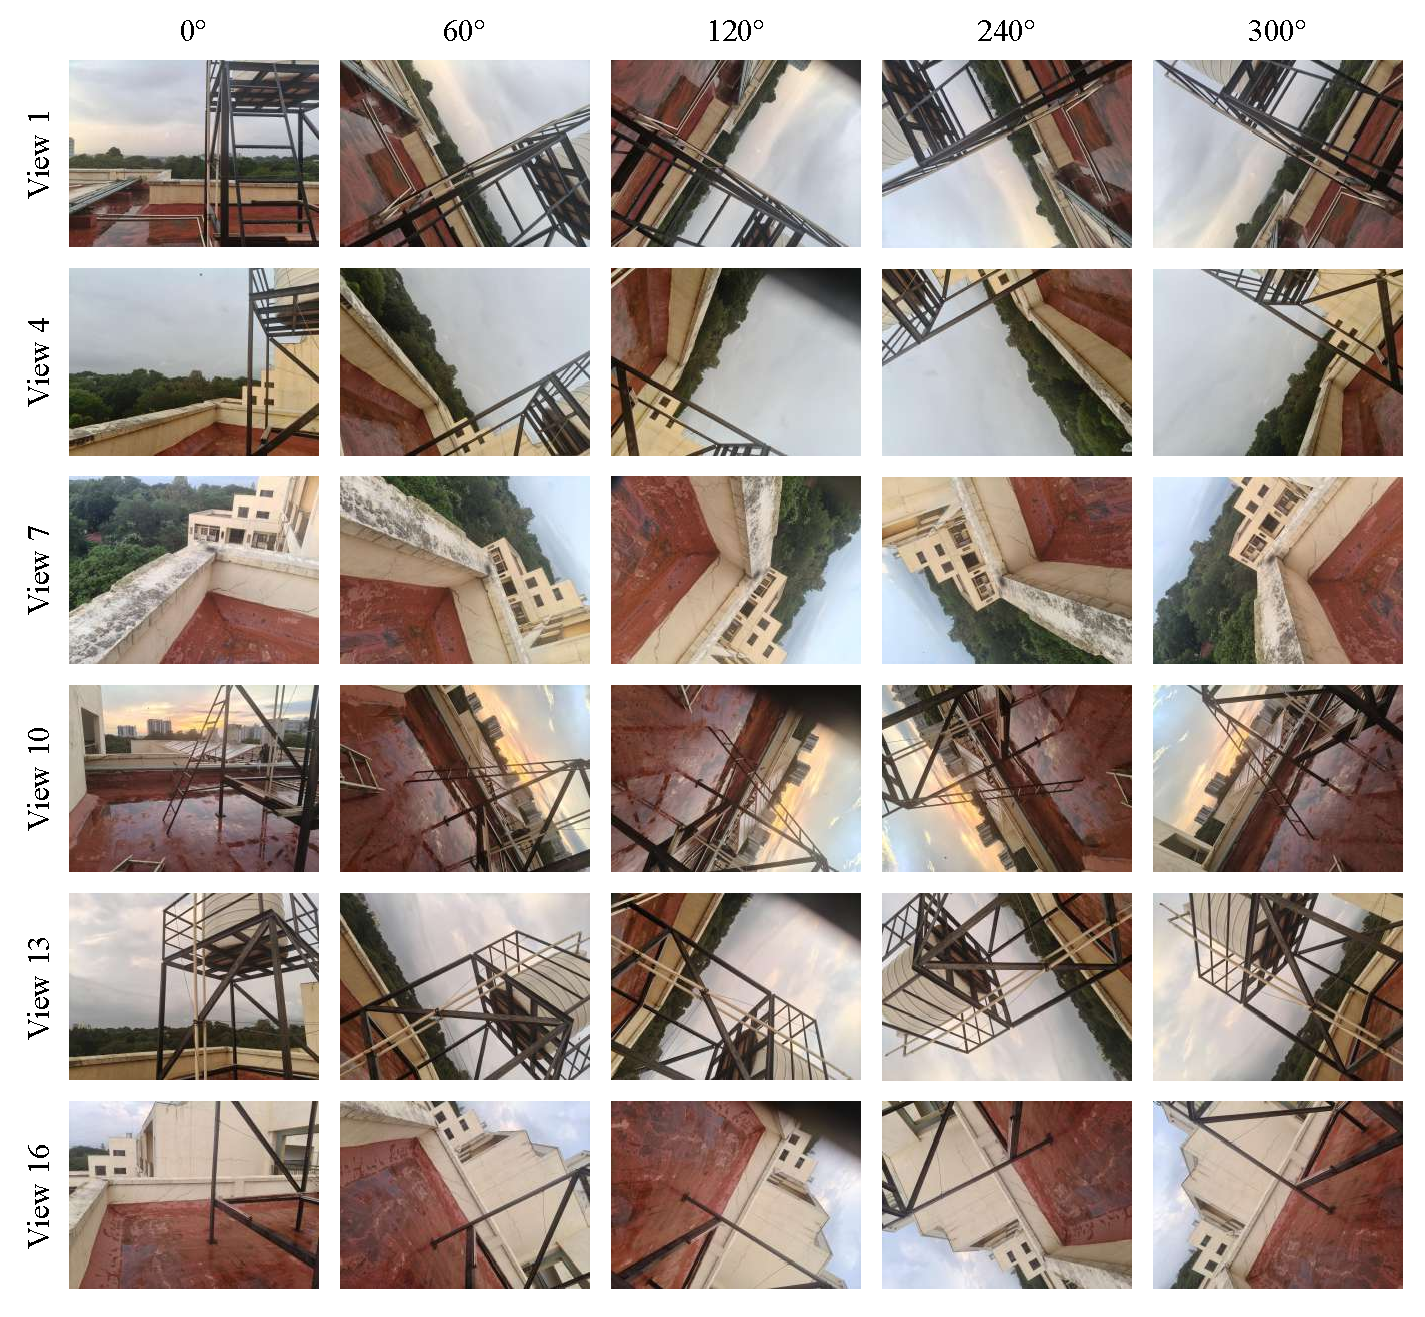
\includegraphics[height=0.47\textheight,keepaspectratio]{Figures/captured_supplementary/rooftop_compressed.pdf}
%   \caption{Rooftop}
%   \label{fig:grid_rooftop}
% \end{subfigure}

% \vspace{1mm}
% \caption{\textbf{ROTMV dataset roll sweeps (Outdoor).} Sampled views (rows) across in-plane roll angles ($0^\circ$- $300^\circ$, columns).}
% \label{fig:grids_outdoor}
% \end{figure*}




\section{Visual Quality Assessment and Rejection Statistics}
\label{sec:image_statistics}
% We render rotated images as described in the algorithm in ~\cref{alg:rotation_generation}. We compare the artifacts produced without and with Difix3D denoising step in ~\Cref{fig:denoise-examples-1} and \Cref{fig:denoise-examples-2}. We observe reconstruction through 3DGS with dense set of images (for ex.: DTU, Mip-NeRF 360) results in good reconstruction, where VisualQuality-R1\citep{wu2026visualquality} outputs a score of $\geq 4.0$ on a scale of $[0-5]$. Therefore, we run Difix3D Denoising only for images generated from the other sparse datasets. After this step, we filter images with artifacts using VisualQuality-R1 pipeline where we pass the rotated image and it's 0° counterpart along with a prompt to provide a quality score in the range $[0-5]$. Thereafter, we manually filter the images to filter out reconstruction with obvious artifacts. We provide the statistics for the generated and filtered images in ~\cref{tab:img_stats}. Additionally, we provide example images from the quality filtering pipeline in ~\cref{fig:quality-filtering}

  We render rotated images as described in \cref{alg:rotation_generation}. To reduce rendering artifacts, we use only the single-step diffusion denoiser (Difix)
  from Difix3D+~\citep{wu2025difix3d}, applied independently to each rendered view as a post-processing step. We compare renders without and with
  this denoising step in \Cref{fig:denoise-examples-1} and \ref{fig:denoise-examples-2}. We observe that 3DGS reconstructions from dense image sets (e.g., DTU and
  Mip-NeRF 360) already yield high-quality renders, for which VisualQuality-R1~\citep{wu2026visualquality} outputs a score of $\geq 4.0$ on a scale of $[0, 5]$.
  Therefore, we apply the Difix denoiser only to images rendered from the remaining, sparser datasets. We then filter images with artifacts using VisualQuality-R1,
  passing each rotated image together with its $0^\circ$ counterpart and a prompt asking for a quality score in the range $[0, 5]$. Finally, we manually remove any
  remaining renders with obvious artifacts. Statistics for the generated and filtered images are given in \cref{tab:img_stats}, and example images from the quality
  filtering pipeline are shown in \cref{fig:quality-filtering}.

  
\begin{table}[tbp]
\centering
\small
\caption{Statistics of VLM (VisualQuality-R1) based and manual rejection during dataset curation using controlled rotation synthesis.}
\label{tab:img_stats}

\resizebox{0.9\linewidth}{!}{%
% \begin{tabular}{lccccc}
% \toprule
% Dataset & Initial images & Rejected by VQ-R1 & Manually reviewed & Manually rejected & Final \\
% \midrule
% Tanks\&Temples & 1{,}802 & 1{,}552 & 250 & 45 & 205 \\
% 7-Scenes       & 4{,}300 & 3{,}950 & 350 & 28 & 322 \\
% NRGBD          & 1{,}101 & 661   & 440 & 67 & 373 \\
% \bottomrule
% \end{tabular}%
% }
\begin{tabular}{lcccc}
\toprule
Dataset & Initial images & Rejected by VQ-R1 & Manually rejected & Final \\
\midrule
Tanks\&Temples & 43{,}248 & 37{,}248 & 1{,}080 & 4{,}920 \\
% 7\text{-}Scenes & 103{,}200 & 94{,}800 & 672 & 7{,}728 \\
NRGBD & 26{,}424 & 15{,}864 & 1{,}608 & 8{,}952 \\
ETH3D          & 10{,}896 & 9550    & 534 & 812 \\
% ETH3d after removing office dataset
\bottomrule
\end{tabular}%
}


\end{table}

% Make figure captions use the same size as the figure labels.
\captionsetup[figure]{font=small}

% ============================================================
% Denoising qualitative examples — page 1
% ============================================================

\begin{figure}[h]
\centering
\small

% \begin{tabular}{ccc}
% \textbf{Reference} &
% \textbf{Rotated (pre-denoise)} &
% \textbf{Denoised (ours)} \\[4pt]

% \includegraphics[width=0.30\linewidth]
% {supplementary_figures/difix3d_pics/eth3d_courtyard_345_0_ref.jpg} &
% \includegraphics[width=0.30\linewidth]
% {supplementary_figures/difix3d_pics/eth3d_courtyard_345_0_raw.jpg} &
% \includegraphics[width=0.30\linewidth]
% {supplementary_figures/difix3d_pics/eth3d_courtyard_345_0_denoised.jpg} \\

% \multicolumn{3}{c}
% {eth3d / courtyard / 345$^\circ$, score 4.25} \\[4pt]


% \includegraphics[width=0.30\linewidth]
% {supplementary_figures/difix3d_pics/eth3d_pipes_345_1_ref.jpg} &
% \includegraphics[width=0.30\linewidth]
% {supplementary_figures/difix3d_pics/eth3d_pipes_345_1_raw.jpg} &
% \includegraphics[width=0.30\linewidth]
% {supplementary_figures/difix3d_pics/eth3d_pipes_345_1_denoised.jpg} \\

% \multicolumn{3}{c}
% {eth3d / pipes / 345$^\circ$, score 4.25} \\[4pt]


% \includegraphics[width=0.30\linewidth]
% {supplementary_figures/difix3d_pics/eth3d_electro_330_2_ref.jpg} &
% \includegraphics[width=0.30\linewidth]
% {supplementary_figures/difix3d_pics/eth3d_electro_330_2_raw.jpg} &
% \includegraphics[width=0.30\linewidth]
% {supplementary_figures/difix3d_pics/eth3d_electro_330_2_denoised.jpg} \\

% \multicolumn{3}{c}
% {eth3d / electro / 330$^\circ$, score 4.20} \\[4pt]


% \includegraphics[width=0.30\linewidth]
% {supplementary_figures/difix3d_pics/eth3d_electro_60_3_ref.jpg} &
% \includegraphics[width=0.30\linewidth]
% {supplementary_figures/difix3d_pics/eth3d_electro_60_3_raw.jpg} &
% \includegraphics[width=0.30\linewidth]
% {supplementary_figures/difix3d_pics/eth3d_electro_60_3_denoised.jpg} \\

% \multicolumn{3}{c}
% {eth3d / electro / 60$^\circ$, score 3.80} \\[4pt]


% \includegraphics[width=0.30\linewidth]
% {supplementary_figures/difix3d_pics/eth3d_pipes_60_4_ref.jpg} &
% \includegraphics[width=0.30\linewidth]
% {supplementary_figures/difix3d_pics/eth3d_pipes_60_4_raw.jpg} &
% \includegraphics[width=0.30\linewidth]
% {supplementary_figures/difix3d_pics/eth3d_pipes_60_4_denoised.jpg} \\

% \multicolumn{3}{c}
% {eth3d / pipes / 60$^\circ$, score 3.80} \\[4pt]

% \end{tabular}
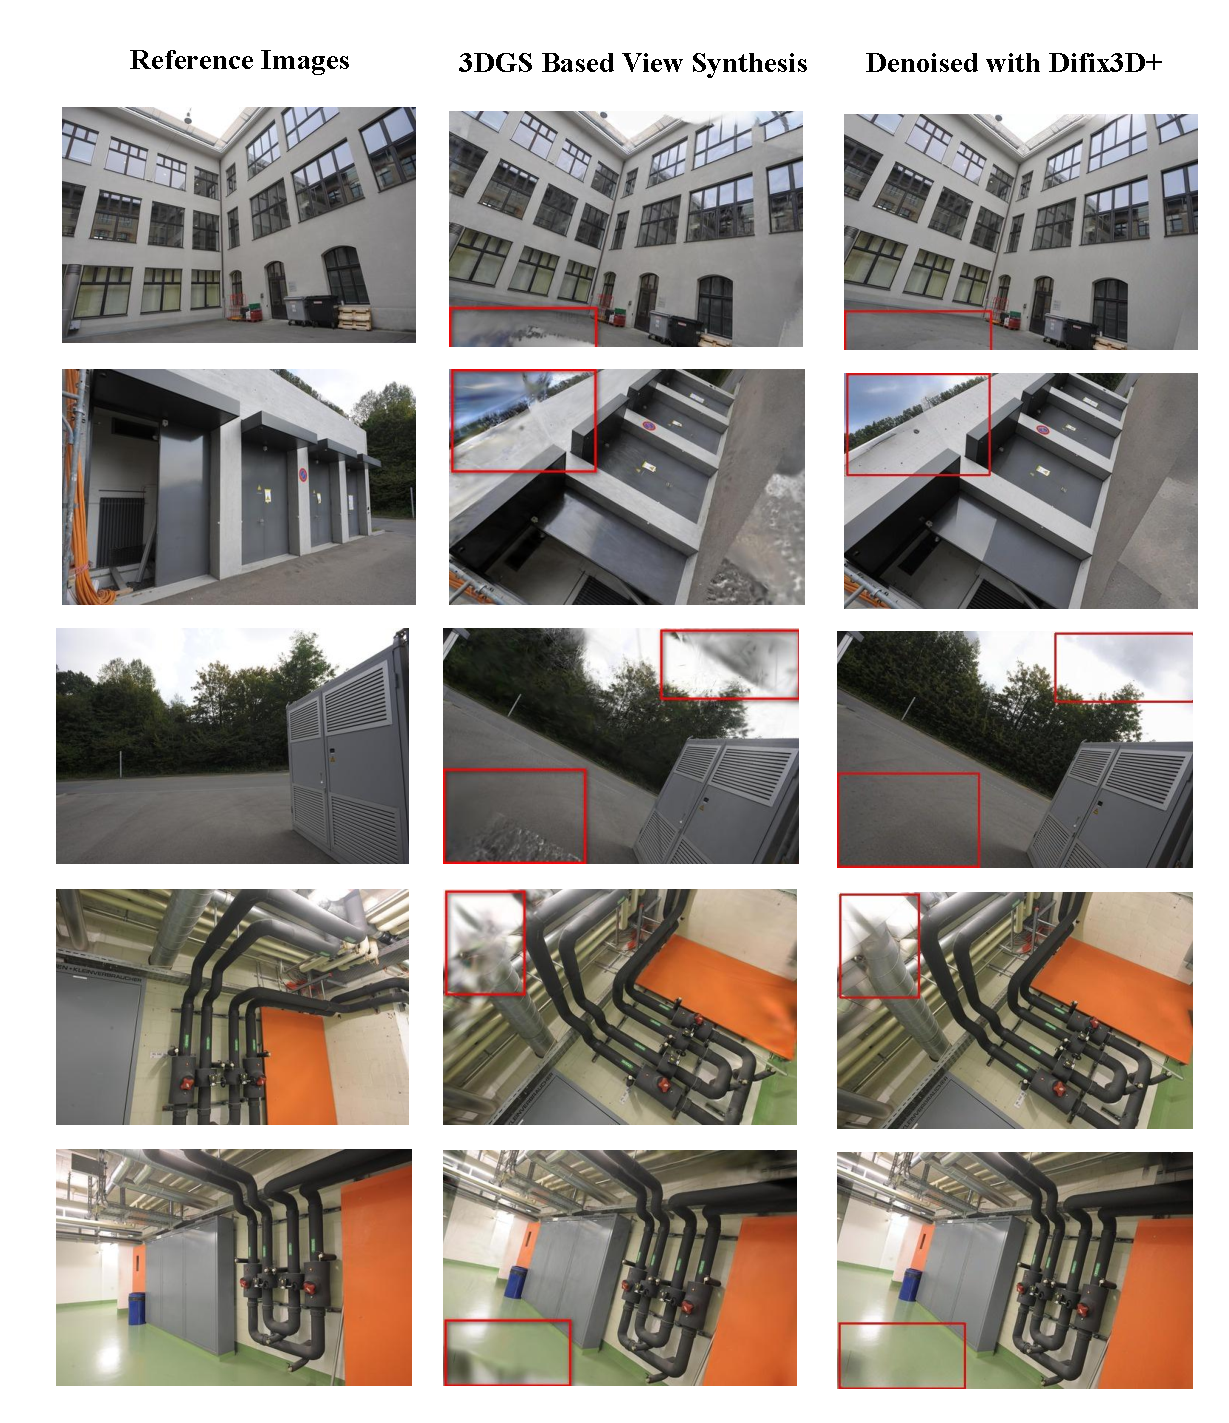
\includegraphics[width=0.98\linewidth,height=0.88\textheight,keepaspectratio]{supplementary_figures/difix3d_examples/difix-1-1.pdf}
\caption{\textbf{Effect of Difix denoising on 3DGS-based rotated view synthesis.} Reference images (left), 3DGS-synthesized views (middle), and their denoised counterparts (right), shown for the \textit{Courtyard}, \textit{Electro} and \textit{Pipes}  scenes from ETH3D. Red boxes mark artifacts in the synthesized views, with corresponding regions in the denoised views to indicate that the artifacts are removed or reduced.}
\label{fig:denoise-examples-1}

\end{figure}


% ============================================================
% Denoising qualitative examples — page 2
% ============================================================

\begin{figure}[h]
% \ContinuedFloat
\centering
\small

% \begin{tabular}{ccc}
% \textbf{Reference} &
% \textbf{Rotated (pre-denoise)} &
% \textbf{Denoised (ours)} \\[4pt]

% \includegraphics[width=0.30\linewidth]
% {supplementary_figures/difix3d_pics/tnt_Meetingroom_roll_15_5_ref.jpg} &
% \includegraphics[width=0.30\linewidth]
% {supplementary_figures/difix3d_pics/tnt_Meetingroom_roll_15_5_raw.jpg} &
% \includegraphics[width=0.30\linewidth]
% {supplementary_figures/difix3d_pics/tnt_Meetingroom_roll_15_5_denoised.jpg} \\

% \multicolumn{3}{c}
% {tnt / Meetingroom / roll 15$^\circ$, score 4.20} \\[4pt]


% \includegraphics[width=0.30\linewidth]
% {supplementary_figures/difix3d_pics/tnt_Meetingroom_roll_15_6_ref.jpg} &
% \includegraphics[width=0.30\linewidth]
% {supplementary_figures/difix3d_pics/tnt_Meetingroom_roll_15_6_raw.jpg} &
% \includegraphics[width=0.30\linewidth]
% {supplementary_figures/difix3d_pics/tnt_Meetingroom_roll_),15_6_denoised.jpg} \\

% \multicolumn{3}{c}
% {tnt / Meetingroom / roll 15$^\circ$, score 4.20} \\[4pt]


% \includegraphics[width=0.30\linewidth]
% {supplementary_figures/difix3d_pics/tnt_Church_roll_15_7_ref.jpg} &
% \includegraphics[width=0.30\linewidth]
% {supplementary_figures/difix3d_pics/tnt_Church_roll_15_7_raw.jpg} &
% \includegraphics[width=0.30\linewidth]
% {supplementary_figures/difix3d_pics/tnt_Church_roll_15_7_denoised.jpg} \\

% \multicolumn{3}{c}
% {tnt / Church / roll 15$^\circ$, score 4.00} \\[4pt]


% \includegraphics[width=0.30\linewidth]
% {supplementary_figures/difix3d_pics/tnt_Church_roll_15_8_ref.jpg} &
% \includegraphics[width=0.30\linewidth]
% {supplementary_figures/difix3d_pics/tnt_Church_roll_15_8_raw.jpg} &
% \includegraphics[width=0.30\linewidth]
% {supplementary_figures/difix3d_pics/tnt_Church_roll_15_8_denoised.jpg} \\

% \multicolumn{3}{c}
% {tnt / Church / roll 15$^\circ$, score 4.00} \\[4pt]

% \end{tabular}
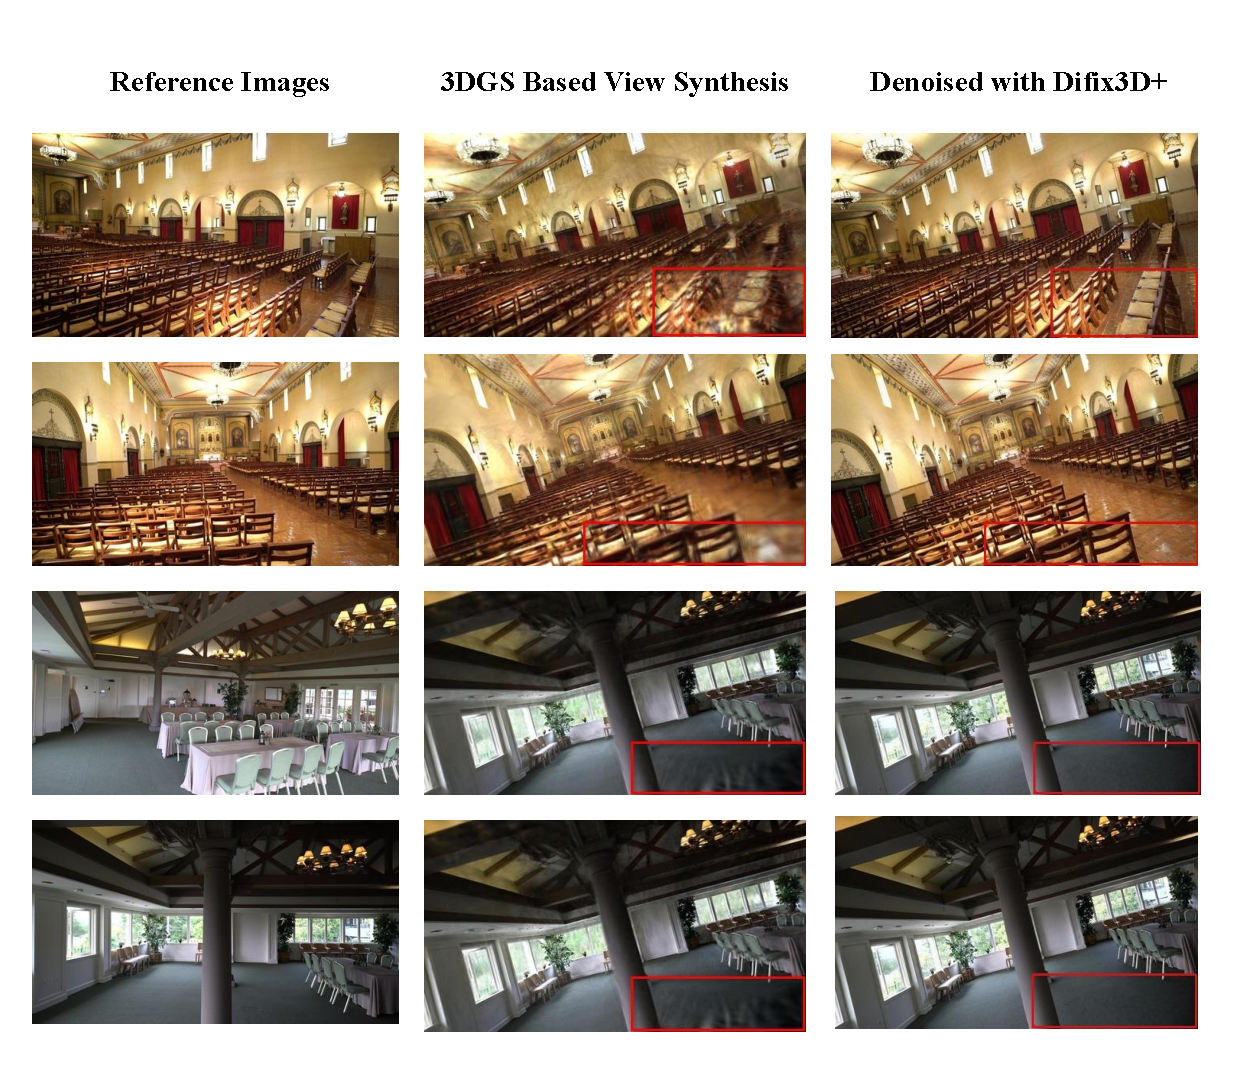
\includegraphics[width=0.98\linewidth,height=0.88\textheight,keepaspectratio]{supplementary_figures/difix3d_examples/difix-2-1.pdf}
\caption{\textbf{Effect of Difix3D denoising on 3DGS-based rotated view synthesis.} Reference images (left), 3DGS-synthesized views (middle), and their denoised counterparts (right), shown for the \textit{Church} and \textit{Meetingroom} scenes from Tanks and Temples. Red boxes mark artifacts in the synthesized views, with corresponding regions in the denoised views to indicate that the artifacts are removed or reduced.}
\label{fig:denoise-examples-2}

\end{figure}

\begin{figure}[!htb]
    \centering
    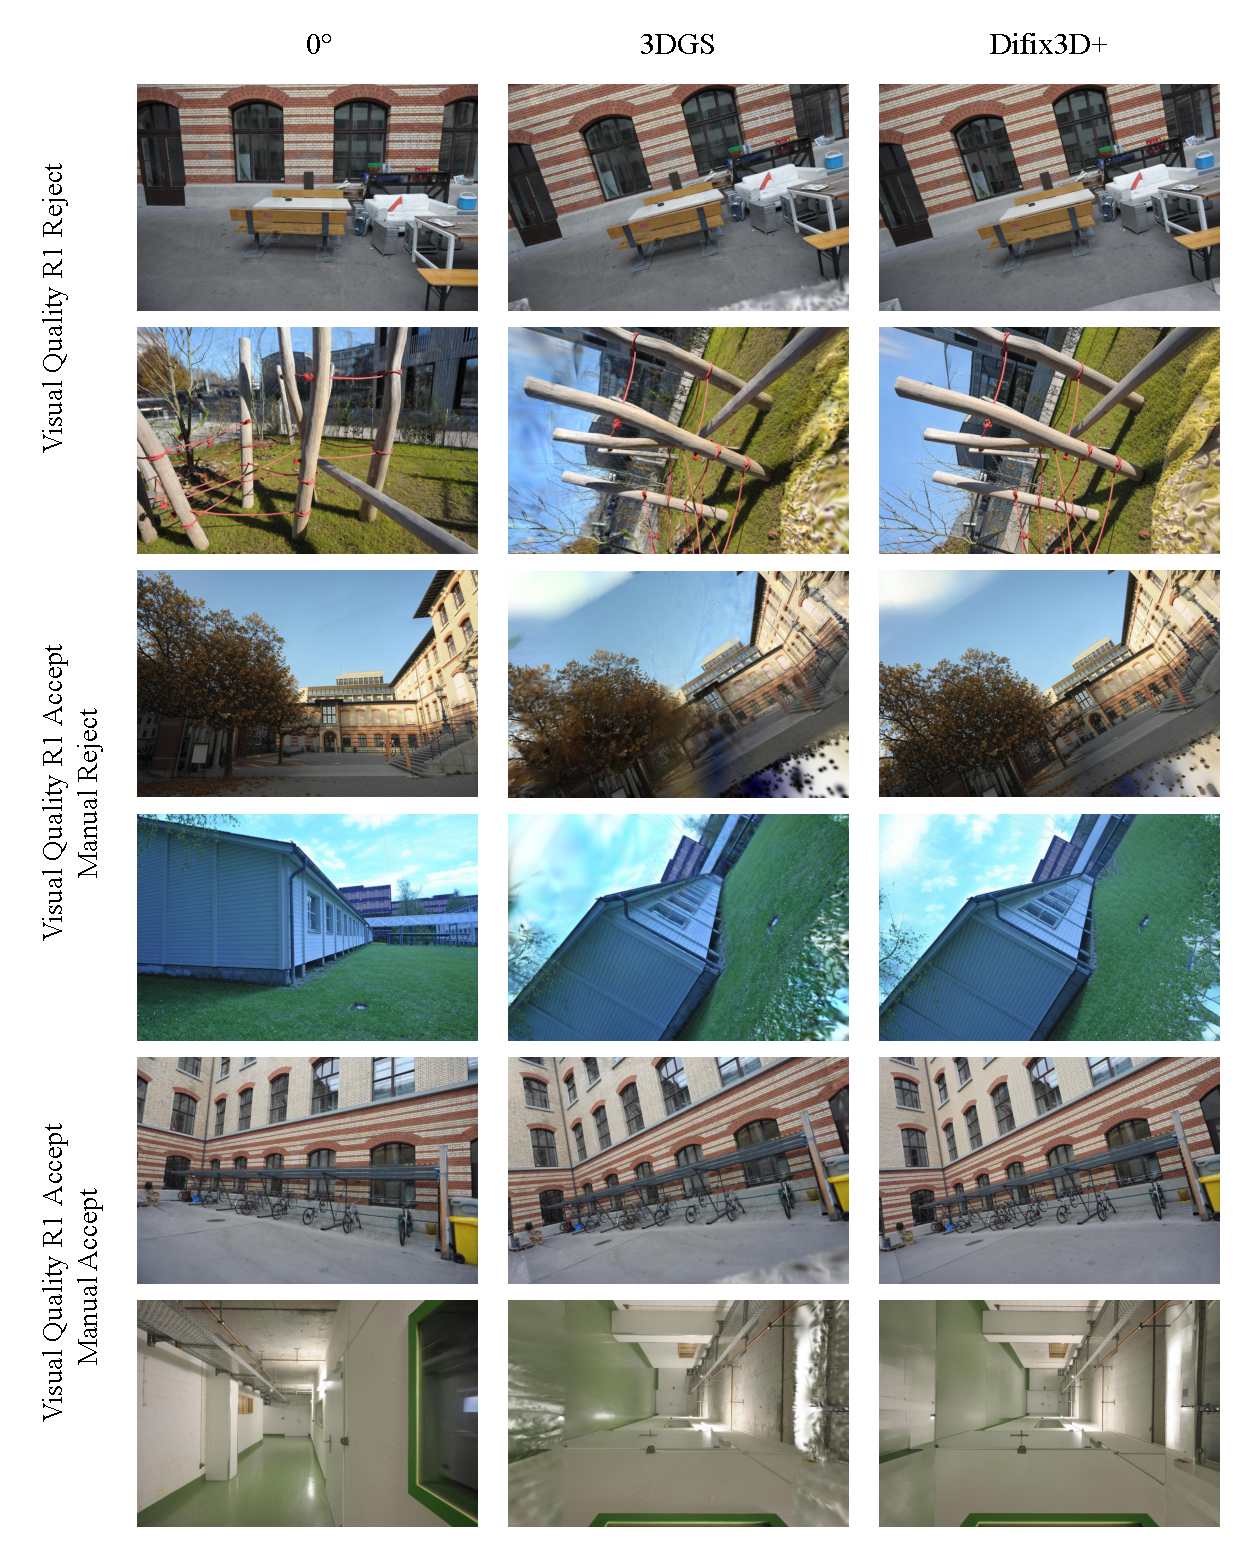
\includegraphics[width=\linewidth,height=0.9\textheight,keepaspectratio]{supplementary_figures/Section_H/SectionH.pdf}
    \caption{Qualitative examples of the quality filtering pipeline across reference ($0^\circ$), raw 3DGS, and Difix-denoised views, showing automated rejections (top), manual rejections (middle), and accepted views (bottom).}
    \label{fig:quality-filtering}
\end{figure}

\section{Failure Case}
\Cref{tab:office_pose} reports pose and point-cloud metrics on ETH3D on the scene \emph{office}. Across other scenes, variance-based roll correction recovers the upright prior and improves the reconstruction, but the \emph{office} scene is a consistent failure case: correction degrades \emph{every} metric for \emph{every} model relative to the baseline. ATE increases uniformly (e.g., $0.040$ to $0.095$ for VGGT-$\Omega$), and both Tacc@30 and Racc@30 fall sharply (e.g., $98.39$ to $63.72$ and $100.00$ to $81.57$ for DA3).

We attribute this failure to rotation to symmetry failure and primarily rotation in pitch and yaw.\Cref{fig:office_failure_qualitative} qualitatively compares the original upright ($0^\circ$) views with the ROVER-corrected views obtained from the corresponding rotated inputs.

\begin{table}[tbp]
\centering
\setlength{\tabcolsep}{3pt}
\caption{Pose estimation results on the ETH3D \emph{office} scene.}
\label{tab:office_pose}
\begin{tabular}{lcccccc}
\toprule
\multirow{2}{*}{Model} & \multicolumn{2}{c}{ATE $\downarrow$} & \multicolumn{2}{c}{Tacc@30 $\uparrow$} & \multicolumn{2}{c}{Racc@30 $\uparrow$} \\
\cmidrule(lr){2-3} \cmidrule(lr){4-5} \cmidrule(lr){6-7}
 & Base & Ours & Base & Ours & Base & Ours \\
\midrule
DA3           & \textbf{0.049} & 0.265 & \textbf{98.39} & 63.72 & \textbf{100.00} & 81.57 \\
MapA          & \textbf{0.236} & 0.313 & \textbf{25.89} & 19.41 & \textbf{92.68}  & 66.75 \\
$\pi^3$       & \textbf{0.208} & 0.326 & \textbf{54.63} & 33.56 & \textbf{92.68}  & 56.40 \\
VGGT          & \textbf{0.157} & 0.241 & \textbf{77.38} & 57.05 & \textbf{92.68}  & 69.49 \\
VGGT-$\Omega$ & \textbf{0.040} & 0.095 & \textbf{96.18} & 86.54 & \textbf{100.00} & 87.50 \\
\bottomrule
\end{tabular}
\end{table}
\raggedbottom
\begin{figure}[H]
    \centering
    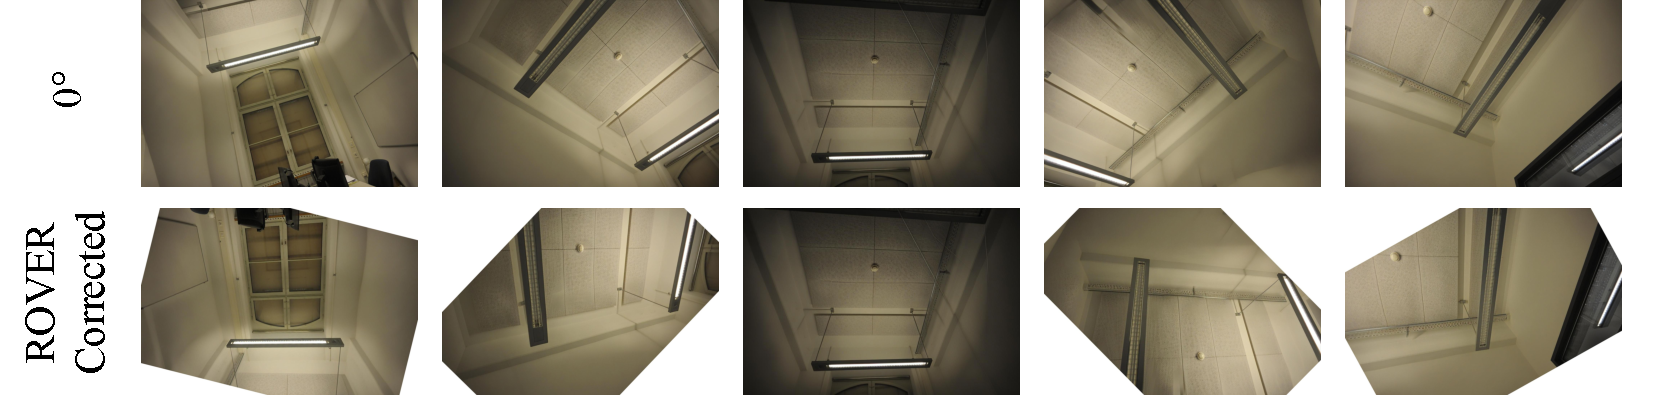
\includegraphics[width=\linewidth, keepaspectratio]{supplementary_figures/eth3d_failcases.pdf}
    \caption{Qualitative failure on the ETH3D \emph{office} scene. Steep upward pitch and ceiling symmetries cause ROVER to introduce spurious corrective rotations to already-upright ($0^\circ$) views.}
    \label{fig:office_failure_qualitative}
\end{figure}

\section{Evaluation Criteria}
\flushbottom
\label{sec:eval_criteria}

Following the protocol described in ~\Cref{sec:algorithm} to generate multi-view scenes with random rotation across frames. We follow the evaluation protocol from \cite{wang2025pi} and evaluate camera pose and point cloud for each rotation configuration set.

\paragraph{Ground-truth pose under roll.}
Let $R$ and $t$ be the $SO(3)$ ground truth rotation matrix and translation vector respectively for a frame. For a roll of $\theta$ about the optical axis, let $\mathbf{R}_z(\theta)$ be the $SO(3)$ rotation matrix about the $z-$axis. Then, under a roll of $\theta$, the world-to-camera pose $[\mathbf{R} \mid \mathbf{t}]$ becomes
$\hat{\mathbf{R}} = \mathbf{R}_z(\theta)\mathbf{R}$ and
$\hat{\mathbf{t}} = \mathbf{R}_z(\theta)\mathbf{t}$. The camera centre
is unchanged,
%
\begin{equation}
-\hat{\mathbf{R}}^{\top}\hat{\mathbf{t}}
= -\mathbf{R}^{\top}\mathbf{R}_z(\theta)^{\top}
   \mathbf{R}_z(\theta)\,\mathbf{t}
= -\mathbf{R}^{\top}\mathbf{t} ,
\label{eq:centre-invariance}
\end{equation}
%
so the ground-truth trajectory is identical to the upright one for
every rotation budget $k$ and angle assignment; the reported ATE
degradation reflects the predicted trajectory alone. Relative
rotations, by contrast, are genuinely re-oriented, so rotation related metrics
are evaluated against altered targets.

\paragraph{Ground-truth geometry under roll.}
Some datasets like ETH3D and DTU provide ground-truth geometry only for the upright
($0^{\circ}$) configuration. Since the scene itself is unchanged by
the roll, we adjust the \emph{support} of the ground truth rather than
its content: the ground-truth depth map $\mathbf{D}$ is rotated in the
image plane, $\hat{\mathbf{D}} = \mathbf{R}_z(\theta)\mathbf{D}$,
regions falling outside the frame after rotation are masked out, and
the remaining pixels are unprojected to 3D using the rotated camera
$[\hat{\mathbf{R}} \mid \hat{\mathbf{t}}]$. This yields the ground-truth
point cloud restricted to the region actually visible in the rotated
view, so that predictions are never penalised for geometry outside the
rolled frustum.

For datasets without ground-truth geometry (Mip-NeRF 360,
RotMV) we take the model's own upright
reconstruction $\hat{\mathbf{P}}_0$ as reference and report the
post-alignment discrepancy of each rotated reconstruction
$\hat{\mathbf{P}}_k$ against it. For our hand-captured dataset no
ground-truth poses are available; we run VGGT on the upright capture
to obtain reference poses and derive the ground truth for each rotated
configuration by composing these with the known roll matrices as in
\eqref{eq:centre-invariance}. These two protocols measure degradation
relative to the model's own upright output rather than absolute
accuracy; our absolute-ground-truth results on 7-Scenes, NRGB-D, ETH3D
and DTU establish the corresponding absolute claims.

\paragraph{Alignment.}
Feed-forward predictions are defined only up to a global similarity
transform. For pose metrics we align the predicted camera centres to
the ground-truth centres with Umeyama. For point
cloud metrics we apply Umeyama followed by ICP to align the predicted
point cloud to the ground truth, following the protocol of
$\pi^3$. All metrics are computed after
alignment.


\paragraph{Pose metrics.}
Let $\mathbf{T}_i, \hat{\mathbf{T}}_i \in SE(3)$ denote the
ground-truth and predicted extrinsics of view $i$, with camera
centres $\mathbf{C}_i, \hat{\mathbf{C}}_i$. After a $\mathrm{Sim}(3)$
trajectory alignment the absolute
trajectory error is
%
\begin{equation}
\mathrm{ATE} = \Big(\tfrac{1}{N}\textstyle\sum_{i=1}^{N}
\big\|\mathbf{C}_i - \hat{\mathbf{C}}_i\big\|_2^2\Big)^{1/2}.
\end{equation}
%
For each of the $\binom{N}{2}$ image pairs $(i,j)$ we form the
relative pose $\Delta\mathbf{T}_{ij} = \mathbf{T}_j\mathbf{T}_i^{-1}$
(and $\Delta\hat{\mathbf{T}}_{ij}$ analogously from
$\hat{\mathbf{T}}_i,\hat{\mathbf{T}}_j$), decomposed into rotation
$\Delta\mathbf{R}_{ij}$ and translation $\mathbf{t}_{ij}$. The
relative rotation error is the geodesic distance
%
\begin{equation}
e^{R}_{ij} = \arccos\!\left(\frac{\mathrm{Tr}\big(\Delta\mathbf{R}_{ij}^{\top}\Delta\hat{\mathbf{R}}_{ij}\big) - 1}{2}\right),
\end{equation}
%
and the relative translation error is the undirected angle between
translation directions (antipodal directions are equivalent, since
scale and sign are unobservable per pair),
%
\begin{equation}
e^{T}_{ij} = \arccos\!\left(\frac{\big|\mathbf{t}_{ij}^{\top}\hat{\mathbf{t}}_{ij}\big|}{\|\mathbf{t}_{ij}\|\,\|\hat{\mathbf{t}}_{ij}\|}\right).
\end{equation}
%

The reported percentages are obtained by thresholding these per-pair errors: $\mathrm{RAcc}_{\tau}$ and $\mathrm{TAcc}_{\tau}$ (Relative Rotation/Translation Accuracy) are the fraction of pairs whose error falls below an angular tolerance $\tau$,
$$\mathrm{RAcc}_{\tau} = \frac{100}{\binom{N}{2}}\sum_{i<j} \mathbbm{1}\left[e^{R}_{ij} < \tau\right], \qquad \mathrm{TAcc}_{\tau} = \frac{100}{\binom{N}{2}}\sum_{i<j} \mathbbm{1}\left[e^{T}_{ij} < \tau\right],$$
reported as percentages; we use $\tau=30^{\circ}$ in the  tables.
The reported AUC uses the \emph{joint} per-pair error
$e^{RT}_{ij} = \max\!\left(e^{R}_{ij}, e^{T}_{ij}\right)$, thresholded
exactly as $\mathrm{RAcc}_\tau$/$\mathrm{TAcc}_\tau$ above,
%
\begin{equation}
\mathrm{Acc}^{\mathrm{joint}}_\tau = \frac{100}{\binom{N}{2}}\sum_{i<j}
\mathbbm{1}\left[e^{RT}_{ij} < \tau\right].
\end{equation}
%
$\mathrm{AUC@}\tau_{\max}$ is the mean of this joint accuracy over
every integer-degree threshold up to $\tau_{\max}$ — a discrete
Riemann-sum approximation, at $1^{\circ}$ resolution, of the area
under the accuracy-vs-threshold curve on $[0^{\circ}, \tau_{\max}]$,
normalised so a perfect predictor scores $100$:
%
\begin{equation}
\mathrm{AUC@}\tau_{\max} = \frac{1}{\tau_{\max}}
\sum_{\tau=1}^{\tau_{\max}} \mathrm{Acc}^{\mathrm{joint}}_\tau .
\end{equation}
%
We report $\mathrm{AUC@30}$ (i.e. $\tau_{\max}=30^{\circ}$) in the
main tables.

\paragraph{Point cloud metrics.}
Following evaluation protocol of $\pi^3$\citep{wang2025pi}, predicted point
maps are aligned to the ground truth with a closed-form
$\mathrm{Sim}(3)$ transform (Umeyama), computed directly from the
pixel-wise correspondence between predicted and ground-truth point
maps, then refined with point-to-point ICP (correspondence threshold
$0.1$--$1.0\,\mathrm{m}$, scaled to each dataset's depth range). Let
$\mathcal{P}$ denote the resulting aligned predicted point cloud and
$\mathcal{Q}$ the ground truth. Accuracy and completeness are the
mean one-sided nearest-neighbour distances,
%
\begin{align}
\mathrm{Acc} &= \tfrac{1}{|\mathcal{P}|}\textstyle\sum_{\mathbf{p}\in\mathcal{P}}
\min_{\mathbf{q}\in\mathcal{Q}}\|\mathbf{p}-\mathbf{q}\|_2 ,
\\[2pt]
\mathrm{Comp} &= \tfrac{1}{|\mathcal{Q}|}\textstyle\sum_{\mathbf{q}\in\mathcal{Q}}
\min_{\mathbf{p}\in\mathcal{P}}\|\mathbf{p}-\mathbf{q}\|_2 ,
\end{align}
%
and their average is the well known Chamfer distance.
Normal consistency (N.C.) is likewise two-sided, averaging the mean absolute
alignment of surface normals at nearest-neighbour correspondences in
each direction,
%
\begin{align}
\mathrm{NC}_1 &= \tfrac{1}{|\mathcal{P}|}\textstyle\sum_{\mathbf{p}\in\mathcal{P}}
\big|\mathbf{n}_{\mathbf{p}} \cdot \mathbf{n}_{\mathrm{nn}_{\mathcal{Q}}(\mathbf{p})}\big| ,
\\[2pt]
\mathrm{NC}_2 &= \tfrac{1}{|\mathcal{Q}|}\textstyle\sum_{\mathbf{q}\in\mathcal{Q}}
\big|\mathbf{n}_{\mathbf{q}} \cdot \mathbf{n}_{\mathrm{nn}_{\mathcal{P}}(\mathbf{q})}\big| ,
\end{align}
%
where $\mathrm{nn}_{\mathcal{X}}(\mathbf{v}) = \arg\min_{\mathbf{x}\in\mathcal{X}}\|\mathbf{v}-\mathbf{x}\|_2$
denotes the nearest neighbour of $\mathbf{v}$ in point set $\mathcal{X}$ (reusing the
correspondences already computed for Acc/Comp above), and $\mathbf{n}_{(\cdot)}$
denotes the surface normal estimated at each point from its local neighbourhood.
We report
\begin{equation}
\mathrm{NC} = \tfrac{1}{2}(\mathrm{NC}_1 + \mathrm{NC}_2) \in [0,1],
\end{equation}
with $\mathrm{NC}=1$ indicating perfectly consistent surface orientation between
prediction and ground truth, and $\mathrm{NC}=0$ indicating orthogonal (maximally
inconsistent) surfaces.



\section{Training Data re-balancing}
\label{sec:training_data_rebalancing}

\Cref{tab:training_data} presents a comprehensive audit of 
the training corpora of all evaluated models. Datasets used by these models are CO3D\citep{co3dv1,reizenstein21co3dv2}, ScanNet/ScanNet++\citep{dai2017scannet, yeshwanthliu2023scannetpp}, MegaDepth\citep{MegaDepthLi18}, DL3DV-10K\citep{ling2024dl3dv}, ARKitScenes\citep{baruch2021arkitscenes}, Mapillary\citep{MapillaryPlanetScaleDepth}, HyperSim\citep{roberts:2021Hypersim}, Habitat/Replica\citep{ramakrishnan2021hm3dhabitat}, Virtual KITTI\citep{gaidon2016virtualkitti2}, BlendedMVS\citep{yao2020blendedmvs}, WildRGB-D\citep{xia2024wildrgbd}, PointOdyssey\citep{zheng2023pointoddessey}, Taskonomy\citep{taskonomy2018}, Waymo Open\cite{Sun_2020_CVPRwaymoopen}, MegaSynth\cite{jiang2024megasynth}, MVS-Synth\citep{DeepMVSSynth}, UnrealStereo4K\citep{zhang2018unrealstereo}, MatrixCity\citep{li2023matrixcity}, Aria Series\citep{pan2023ariadigitaltwin, banerjee2024ariaHOT3D, ma2024arianymeriadataset, lv2024ariaeverydayactivities}, Dynamic Replica\citep{karaev2023dynamicreplicastereo}, Spring\citep{mehl2023springdataset}, Structured3D\citep{Structured3Ddataset}, Cityscapes\cite{cordts2016cityscapes}, GTA-SfM\citep{cao2020longgtasfm}, Kubric\citep{greff2021kubricdataset}, TartanAir\citep{tartanair2020iros} and Mid-Air \citep{Fonder2019MidAir} datasets. Across \textbf{27} datasets spanning indoor RGB-D scans, outdoor photo collections, driving sequences, and synthetic renderings, the overwhelming majority are upright by construction with each model trained on between 10 and 19 fully upright datasets and at most 2 partially aligned ones. This confirms that UprightBias is a data-driven phenomenon: feed-forward models inadvertently absorb a strong canonical orientation prior simply by virtue of what their training data looks like.
\begin{table}[t]
\centering
\caption{Training datasets used by each feed-forward geometric model and their upright alignment status. \checkmark~=~fully upright; $\sim$~=~partially upright The overwhelming majority of training data across all models is upright by construction}
\label{tab:training_data}
\small
\resizebox{\linewidth}{!}{
\begin{tabular}{llccccccc}
\toprule
\textbf{Dataset} & 
\textbf{Capture Modality} & 
\textbf{Upright} & 
\textbf{VGGT} & 
\textbf{VGGT-$\Omega$} & 
\textbf{DA3} & 
\textbf{MapA.} & 
\textbf{$\pi^3$} \\
\midrule
CO3D               & Handheld object-centric video      & \checkmark & \checkmark & \checkmark & \checkmark &            & \checkmark \\
ScanNet / ScanNet++  & Handheld RGB-D indoor scan         & \checkmark & \checkmark & \checkmark & \checkmark & \checkmark & \checkmark \\
MegaDepth            & Internet landmark photography      & \checkmark & \checkmark & \checkmark & \checkmark & \checkmark & \checkmark \\
DL3DV-10K            & Scene-level video                  & \checkmark & \checkmark & \checkmark & \checkmark & \checkmark &            \\
ARKitScenes          & iPad indoor capture                & \checkmark &            & \checkmark & \checkmark &            & \checkmark \\
Mapillary            & Street-level vehicle camera        & \checkmark & \checkmark & \checkmark &            & \checkmark &            \\
HyperSim             & Synthetic indoor rendering         & \checkmark & \checkmark & \checkmark & \checkmark &            & \checkmark \\
Habitat / Replica    & Simulated indoor environments      & \checkmark & \checkmark & \checkmark & \checkmark &            & \checkmark \\
Virtual KITTI        & Driving simulation                 & \checkmark & \checkmark & \checkmark & \checkmark &            &            \\
BlendedMVS           & SfM outdoor/indoor photos          & \checkmark & \checkmark &            & \checkmark & \checkmark & \checkmark \\
WildRGB-D            & In-the-wild RGBD video             & \checkmark & \checkmark & \checkmark & \checkmark &            & \checkmark \\
PointOdyssey         & Synthetic ground-level motion      & \checkmark & \checkmark & \checkmark & \checkmark &            &            \\
Taskonomy            & Indoor scene photography           & \checkmark &            & \checkmark & \checkmark &            & \checkmark \\
Waymo Open               & Autonomous driving cameras         & \checkmark &            & \checkmark & \checkmark &            &            \\
MegaSynth            & Synthetic scene rendering          & \checkmark &            & \checkmark & \checkmark &            &            \\
MVS-Synth            & Synthetic multi-view stereo        & \checkmark & \checkmark & \checkmark & \checkmark & \checkmark &            \\
UnrealStereo4K       & Synthetic indoor/outdoor           & \checkmark &            & \checkmark & \checkmark & \checkmark &            \\
MatrixCity           & Synthetic city aerial/ground       & \checkmark &            &            & \checkmark &            & \checkmark \\
Aria Series          & Egocentric wearable capture        & \checkmark & \checkmark & \checkmark &            & \checkmark &            \\
Dynamic Replica      & Synthetic dynamic indoor           & \checkmark &            & \checkmark &            & \checkmark &            \\
Spring               & Synthetic outdoor driving          & \checkmark &            &            &            & \checkmark &            \\
Structured3D         & Synthetic indoor rendering         & \checkmark &            &            & \checkmark &            &            \\
Cityscapes           & Driving forward-facing camera      & \checkmark &            &            & \checkmark &            &            \\
GTA-SfM              & Game engine driving scenes         & \checkmark &            &            &            &            & \checkmark \\
\midrule
Kubric               & Synthetic random viewpoints        & $\sim$     & \checkmark &            &            &            &            \\
TartanAir            & Drone and aerial simulation        & $\sim$     &            & \checkmark & \checkmark &            & \checkmark \\
Mid-Air              & Drone aerial footage               & $\sim$     &            & \checkmark &            &            & \checkmark \\
\midrule
\multicolumn{2}{l}{\textbf{Fully upright datasets used}} 
& & \textbf{13} & \textbf{18} & \textbf{19} & \textbf{10} & \textbf{11} \\
\multicolumn{2}{l}{\textbf{Partially upright datasets used}} 
& & \textbf{1} & \textbf{2} & \textbf{1} & \textbf{0} & \textbf{2} \\
\bottomrule
\end{tabular}
}
\end{table}
To investigate if re-balancing the training data and finetuning the model recovers the performance we fine-tune $\pi^3$ on a re-balanced version of the DTU training set 
augmented with randomly rotated multi-view sequences, and evaluate 
on the DTU test set under the same rotated-input protocol used 
throughout the paper. Tables~\Cref{tab:pointmap_pi3_variants_dtu} 
and~\Cref{tab:pose_pi3_variants_dtu} report point-map and camera 
pose metrics respectively for the pretrained and fine-tuned models 
across four test scenes. The results do not support the re-balancing hypothesis. 
Fine-tuning yields inconsistent changes, consistent with the feature-distortion risk discussed in \Cref{sec:ROVER_detail}\citep{kumar2022finetuningchallenges, tang2020longchallenges, kang2019decouplingtrainingdata3}. More specifically fine-tuning on rotated data disrupts the DINOv2-derived visual representations that $\pi^3$ relies on, as the rotated fine-tuning distribution diverges from the DINOv2 pretraining distribution. 

% \newcommand{\result}[2]{%
%   \makecell{#1\\[-2pt]{\scriptsize $\pm$#2}}%
% }

% \newcommand{\bestresult}[2]{%
%   \makecell{\bfseries #1\\[-2pt]{\scriptsize $\mathbf{\pm #2}$}}%
% }

% \begin{table}[H]
% \centering
% \caption{
% DTU test-scene point-cloud metrics for the $\pi^3$ backbone.
% Results are reported as mean $\pm$ standard deviation over 50 rotation
% sets per scene. PT denotes pretrained, PT+VC applies DINOv2 variance
% correction, and FT denotes finetuning (v2). Best results are bold.
% }
% \label{tab:pointmap_pi3_variants_dtu}

% \setlength{\tabcolsep}{4.2pt}
% \renewcommand{\arraystretch}{1.12}
% \small

% \begin{tabular}{l ccc ccc ccc}
% \toprule
% \multirow{2}{*}{Scene}
% & \multicolumn{3}{c}{Accuracy $\downarrow$}
% & \multicolumn{3}{c}{Completeness $\downarrow$}
% & \multicolumn{3}{c}{Normal Consistency $\uparrow$} \\
% \cmidrule(lr){2-4}
% \cmidrule(lr){5-7}
% \cmidrule(lr){8-10}
% & PT & PT+VC(Ours) & FT
% & PT & PT+VC(Ours) & FT
% & PT & PT+VC(Ours) & FT \\
% \midrule    

% scan1
% & \result{0.923}{0.311}
% & \bestresult{0.797}{0.269}
% & \result{2.251}{0.279}
% & \result{0.902}{0.281}
% & \bestresult{0.828}{0.238}
% & \result{1.347}{0.161}
% & \result{0.646}{0.009}
% & \result{0.643}{0.007}
% & \bestresult{0.652}{0.006}
% \\

% scan10
% & \result{5.701}{6.254}
% & \result{5.044}{5.790}
% & \bestresult{4.340}{1.000}
% & \result{4.463}{9.323}
% & \bestresult{3.511}{6.707}
% & \result{4.057}{0.704}
% & \result{0.655}{0.020}
% & \result{0.652}{0.022}
% & \bestresult{0.681}{0.013}
% \\

% scan118
% & \result{3.384}{2.605}
% & \result{1.841}{1.423}
% & \bestresult{1.467}{0.272}
% & \result{5.969}{9.243}
% & \result{3.183}{7.865}
% & \bestresult{1.493}{0.286}
% & \result{0.593}{0.039}
% & \bestresult{0.610}{0.028}
% & \result{0.608}{0.004}
% \\

% scan77
% & \bestresult{5.962}{1.011}
% & \result{6.149}{1.069}
% & \result{7.931}{1.186}
% & \bestresult{6.658}{1.894}
% & \result{6.938}{1.831}
% & \result{12.447}{2.721}
% & \result{0.622}{0.010}
% & \bestresult{0.628}{0.012}
% & \result{0.607}{0.007}
% \\

% \bottomrule
% \end{tabular}
% \end{table}

%%%%%%%%%%%%%%%%%%%%%%%%%%%%%%%%%%%%%%%%%%%%%%%%%%%%%%%%%%%%%%%%%%%%%%%%%%%%%%%%%%%%%%%%%%%%%%%%%%%%%%%%%%%%%%%%%%%%%%%%%%%%%%%%%%%%%%%%%%%%%%%%%%%%%%%%%%%%%%%%%%%%%%%%%%%%%%%%%%%%%%%%%%%%%%%%%%%%%%%%%%%%%%%%%%%%%%%%%%%%%%%%%%%%%%%%%%%%%%%%

\newcommand{\result}[2]{%
  \makecell{#1\\[-2pt]{\scriptsize $\pm$#2}}%
}

\newcommand{\bestresult}[2]{%
  \makecell{\bfseries #1\\[-2pt]{\scriptsize $\mathbf{\pm #2}$}}%
}

\begin{table}[H]
\centering
\caption{
DTU test-scene point-cloud metrics for the $\pi^3$ backbone finetuning with rebalanced dataset.
Results are reported as mean $\pm$ standard deviation over 50 rotation
sets per scene. We compare the pretrained model with the finetuned
model.
}
\label{tab:pointmap_pi3_variants_dtu}

\setlength{\tabcolsep}{4.2pt}
\renewcommand{\arraystretch}{1.12}
\small

\begin{tabular}{l cc cc cc}
\toprule
\multirow{2}{*}{Scene}
& \multicolumn{2}{c}{Accuracy $\downarrow$}
& \multicolumn{2}{c}{Completeness $\downarrow$}
& \multicolumn{2}{c}{Normal Consistency $\uparrow$} \\
\cmidrule(lr){2-3}
\cmidrule(lr){4-5}
\cmidrule(lr){6-7}
& Pretrained & Finetuned
& Pretrained & Finetuned
& Pretrained & Finetuned \\
\midrule    

scan1
& \bestresult{0.923}{0.311}
& \result{2.251}{0.279}
& \bestresult{0.902}{0.281}
& \result{1.347}{0.161}
& \result{0.646}{0.009}
& \bestresult{0.652}{0.006}
\\

scan10
& \result{5.701}{6.254}
& \bestresult{4.340}{1.000}
& \result{4.463}{9.323}
& \bestresult{4.057}{0.704}
& \result{0.655}{0.020}
& \bestresult{0.681}{0.013}
\\

scan118
& \result{3.384}{2.605}
& \bestresult{1.467}{0.272}
& \result{5.969}{9.243}
& \bestresult{1.493}{0.286}
& \result{0.593}{0.039}
& \bestresult{0.608}{0.004}
\\

scan77
& \bestresult{5.962}{1.011}
& \result{7.931}{1.186}
& \bestresult{6.658}{1.894}
& \result{12.447}{2.721}
& \bestresult{0.622}{0.010}
& \result{0.607}{0.007}
\\

\bottomrule
\end{tabular}
\end{table}
% \begin{table}[H]
% \centering

% % Local result-cell definitions
% \def\result#1#2{%
%   \makecell{#1\\[-2pt]{\scriptsize $\pm$#2}}%
% }
% \def\bestresult#1#2{%
%   \makecell{\bfseries #1\\[-2pt]{\scriptsize $\mathbf{\pm #2}$}}%
% }

% \caption{
% DTU test-scene pose metrics for the $\pi^3$ backbone.
% Results are reported as mean $\pm$ standard deviation over 50 rotation
% sets per scene. PT denotes pretrained, PT+VC applies DINOv2 variance
% correction, and FT denotes finetuning (v2). Best results are bold.
% }
% \label{tab:pose_pi3_variants_dtu}

% \setlength{\tabcolsep}{7pt}
% \renewcommand{\arraystretch}{1.12}
% \small

% \begin{tabular}{l ccc ccc}
% \toprule
% \multirow{2}{*}{Scene}
% & \multicolumn{3}{c}{ATE $\downarrow$}
% & \multicolumn{3}{c}{AUC@30 $\uparrow$} \\
% \cmidrule(lr){2-4}
% \cmidrule(lr){5-7}
% & PT & PT+VC(Ours) & FT
% & PT & PT+VC(Ours) & FT \\
% \midrule

% scan1
% & \result{9.161}{3.658}
% & \bestresult{6.805}{2.481}
% & \result{10.550}{3.293}
% & \result{94.832}{2.343}
% & \bestresult{96.351}{1.534}
% & \result{94.073}{1.927}
% \\

% scan10
% & \result{72.433}{77.302}
% & \result{64.940}{61.045}
% & \bestresult{34.919}{4.356}
% & \result{77.543}{18.736}
% & \bestresult{78.684}{13.282}
% & \result{61.702}{3.774}
% \\

% scan118
% & \result{79.647}{88.556}
% & \result{37.851}{65.303}
% & \bestresult{17.696}{3.658}
% & \result{81.022}{17.060}
% & \bestresult{90.468}{5.708}
% & \result{86.688}{3.347}
% \\

% scan77
% & \result{49.597}{41.676}
% & \bestresult{39.541}{43.088}
% & \result{206.479}{64.354}
% & \result{77.976}{12.527}
% & \bestresult{84.647}{6.890}
% & \result{26.733}{9.703}
% \\

% \bottomrule
% \end{tabular}
% \end{table}


%%%%%%%%%%%%%%%%%%%%%%%%%%%%%%%%%%%%%%%%%%%%%%%%%%%%%%%%%%%%%%%%%%%%%%%%%%%%%%%%%%%%%%%%%%%%%%%%%%%%%%%%%%%%%%%%%%%%%%


\begin{table}[tbp]
\centering

% Local result-cell definitions
\def\result#1#2{%
  \makecell{#1\\[-2pt]{\scriptsize $\pm$#2}}%
}
\def\bestresult#1#2{%
  \makecell{\bfseries #1\\[-2pt]{\scriptsize $\mathbf{\pm #2}$}}%
}

\caption{
DTU test-scene pose metrics for the $\pi^3$ backbone finetuning with rebalanced dataset.
Results are reported as mean $\pm$ standard deviation over 50 rotation
sets per scene. We compare the pretrained model with the finetuned (v2)
model.
}
\label{tab:pose_pi3_variants_dtu}

\setlength{\tabcolsep}{7pt}
\renewcommand{\arraystretch}{1.12}
\small

\begin{tabular}{l cc cc}
\toprule
\multirow{2}{*}{Scene}
& \multicolumn{2}{c}{ATE $\downarrow$}
& \multicolumn{2}{c}{$\text{AUC}_{30}$ $\uparrow$} \\
\cmidrule(lr){2-3}
\cmidrule(lr){4-5}
& Pretrained & Finetuned
& Pretrained & Finetuned \\
\midrule

scan1
& \bestresult{9.161}{3.658}
& \result{10.550}{3.293}
& \bestresult{94.832}{2.343}
& \result{94.073}{1.927}
\\

scan10
& \result{72.433}{77.302}
& \bestresult{34.919}{4.356}
& \bestresult{77.543}{18.736}
& \result{61.702}{3.774}
\\

scan118
& \result{79.647}{88.556}
& \bestresult{17.696}{3.658}
& \result{81.022}{17.060}
& \bestresult{86.688}{3.347}
\\

scan77
& \bestresult{49.597}{41.676}
& \result{206.479}{64.354}
& \bestresult{77.976}{12.527}
& \result{26.733}{9.703}
\\

\bottomrule
\end{tabular}
\end{table}


\section{Outlier Detection using RobustVGGT}
\label{sec:outlier_detection_robustvggt}

% \section{Relational Feature and Attention-Based Rotation Identification}
% \label{sec:attentionbased_rotation_detection}

% In-plane frame rotations disrupt spatial feature correlations in feed-forward models, degrading camera pose estimation.
% Inspired by RobustVGGT~\citep{robustvggt}, we identify rotated frames in a zero-shot manner directly from internal network features. Specifically, we extract spatial patch tokens $\mathbf{X}_i \in \mathbb{R}^{P \times D}$ and multi-head query-key projections $\mathbf{Q}_i, \mathbf{K}_i \in \mathbb{R}^{H \times P \times d_k}$ from the first global self-attention layer across an $N$-frame sequence during a single forward pass.

% \subsection{Relational Representation Matrix}
% For each frame pair $(i, j)$, we evaluate inter-frame consistency through token similarity and global attention:
% \begin{equation}
% C_{i,j} = \frac{1}{P^2} \sum_{p,q=1}^{P} \frac{\langle \mathbf{X}_{i,p}, \mathbf{X}_{j,q} \rangle}{\|\mathbf{X}_{i,p}\|_2 \|\mathbf{X}_{j,q}\|_2}, \qquad
% A_{i,j} = \frac{1}{H P} \sum_{h=1}^{H} \sum_{p=1}^{P} \operatorname{Softmax}\left( \frac{\mathbf{Q}_{i,p}^{(h)} (\mathbf{K}_j^{(h)})^\top}{\sqrt{d_k}} \right).
% \end{equation}
% Both matrices are min-max normalized to $[0, 1]$ across all frame pairs using a small constant $\epsilon = 10^{-6}$ for numerical stability, yielding normalized matrices $\mathbf{C}'$ and $\mathbf{A}'$. We construct the joint symmetric affinity matrix as $\mathbf{M} = \frac{1}{2}(\mathbf{C}' + \mathbf{A}') \in \mathbb{R}^{N \times N}$.

% \subsection{Sequence-Level Rotation Detection}
% To detect orientation anomalies, we define a sequence reference profile $\mathbf{T} \in \mathbb{R}^N$ by taking the column-wise median across frames, $T_j = \operatorname{median}_{i}(M_{i,j})$, and compute each frame's mean absolute deviation:
% \begin{equation}
% d_i = \frac{1}{N} \sum_{j=1}^{N} |M_{i,j} - T_j|.
% \end{equation}
% Frames are sorted in descending order of deviation: $\mathbf{d}_{\text{sorted}} = [d_{\pi(1)}, \dots, d_{\pi(N)}]$. We partition the sequence under two orientation priors:
% \begin{itemize}
%     \item \textbf{Minority Rotation (Gap-Based):} Assuming rotated frames form an anomalous minority ($k \le \lfloor N/2 \rfloor$), the decision boundary is placed at the largest consecutive deviation drop:
%     \begin{equation}
%     k^* = \arg\max_{1 \le k \le \lfloor N/2 \rfloor} (d_{\pi(k)} - d_{\pi(k+1)}).
%     \end{equation}
%     The top $k^*$ frames $\{\pi(1), \dots, \pi(k^*)\}$ are classified as \textbf{rotated}, while the remaining $N - k^*$ frames are labeled as \textbf{upright}.

%     \item \textbf{Majority Rotation (Variance Minimization):} When rotated frames dominate, the reference profile $\mathbf{T}$ reflects the rotated orientation, making upright frames appear as high-deviation outliers. We partition the sequence into candidate upright frames $G_{\text{up}} = \{d_{\pi(1)}, \dots, d_{\pi(k)}\}$ and rotated frames $G_{\text{rot}} = \{d_{\pi(k+1)}, \dots, d_{\pi(N)}\}$. Sweeping $k \in [1, \min(8, N-1)]$, the optimal split $k^*$ minimizes the within-class variance:
%     \begin{equation}
%     \sigma^2_w(k) = \frac{k}{N} \sigma^2(G_{\text{up}}) + \frac{N - k}{N} \sigma^2(G_{\text{rot}}).
%     \end{equation}
%     The top $k^*$ frames are isolated as \textbf{upright}, and the remaining $N - k^*$ frames are classified as \textbf{rotated}.
% \end{itemize}

% \subsection{Sensitivity to the Rotation Prior}
% As shown in Table~\Cref{tab:rotation-prior}, detection is substantially more reliable when rotated frames form the minority (average Global F1 of $0.811$ vs.\ $0.543$ under the majority setting). Precision and recall both degrade when canonical reference frames become scarce, demonstrating the necessity of an upright reference anchor for unsupervised relational profiling.
A natural alternative to correcting rotated views is to detect and discard them. As noted in \cref{sec:ablation}, we evaluate this strategy using RobustVGGT~\citep{robustvggt}, which flags views that are inconsistent with the rest of the sequence and excludes them before reconstruction. Unlike ROVER, which estimates the orientation of each view independently, this approach relies on relations between views. Following  RobustVGGT , we identify rotated frames in a zero-shot manner directly from the model's internal feature representations. Specifically, we extract spatial patch tokens $\mathbf{X}_i \in \mathbb{R}^{N_p \times D_{\text{feat}}}$ and multi-head query-key projections $\mathbf{Q}_i, \mathbf{K}_i \in \mathbb{R}^{H \times N_p \times d_k}$ from the first global self-attention layer across an $N$-frame sequence during a single forward pass.

\subsection{Relational Representation Matrix}
For each frame pair $(i, j)$, we evaluate inter-frame consistency through token similarity and global attention:
\begin{equation}
S_{i,j} = \frac{1}{N_p^2} \sum_{u,v=1}^{N_p} \frac{\langle \mathbf{X}_{i,u}, \mathbf{X}_{j,v} \rangle}{\|\mathbf{X}_{i,u}\|_2 \|\mathbf{X}_{j,v}\|_2}, \qquad
A_{i,j} = \frac{1}{H N_p} \sum_{h=1}^{H} \sum_{u=1}^{N_p} \operatorname{Softmax}\left( \frac{\mathbf{Q}_{i,u}^{(h)} (\mathbf{K}_j^{(h)})^\top}{\sqrt{d_k}} \right).
\end{equation}
Both matrices are min-max normalized to $[0, 1]$ across all frame pairs using a small constant $\epsilon = 10^{-6}$ for numerical stability, yielding normalized matrices $\mathbf{S}'$ and $\mathbf{A}'$. We construct the joint symmetric affinity matrix as $\mathbf{W} = \frac{1}{2}(\mathbf{S}' + \mathbf{A}') \in \mathbb{R}^{N \times N}$.

\subsection{Sequence-Level Rotation Detection}
To detect orientation anomalies, we define a sequence reference profile $\mathbf{r} \in \mathbb{R}^N$ by taking the column-wise median across frames, $r_j = \operatorname{median}_{i}(W_{i,j})$, and compute each frame's mean absolute deviation:
\begin{equation}
d_i = \frac{1}{N} \sum_{j=1}^{N} |W_{i,j} - r_j|.
\end{equation}
Frames are sorted in descending order of deviation: $\mathbf{d}_{\text{sorted}} = [d_{\rho(1)}, \dots, d_{\rho(N)}]$. We partition the sequence under two orientation priors:

$\bullet$ \textbf{Minority Rotation (Gap-Based):} Assuming rotated frames form an anomalous minority ($s \le \lfloor N/2 \rfloor$), the decision boundary is placed at the largest consecutive deviation drop:
    \begin{equation}
    s^* = \arg\max_{1 \le s \le \lfloor N/2 \rfloor} (d_{\rho(s)} - d_{\rho(s+1)}).
    \end{equation}
    The top $s^*$ frames $\{\rho(1), \dots, \rho(s^*)\}$ are classified as \textbf{rotated}, while the remaining $N - s^*$ frames are labeled as \textbf{upright}.

$\bullet$ \textbf{Majority Rotation (Variance Minimization):} When rotated frames dominate, the reference profile $\mathbf{r}$ reflects the rotated orientation, making upright frames appear as high-deviation outliers. We partition the sequence into candidate upright frames $G_{\text{up}} = \{d_{\rho(1)}, \dots, d_{\rho(s)}\}$ and rotated frames $G_{\text{rot}} = \{d_{\rho(s+1)}, \dots, d_{\rho(N)}\}$. Sweeping $s \in [1, \min(8, N-1)]$, the optimal split $s^*$ minimizes the within-class variance:
    \begin{equation}
    \sigma^2_w(s) = \frac{s}{N} \sigma^2(G_{\text{up}}) + \frac{N - s}{N} \sigma^2(G_{\text{rot}}).
    \end{equation}
    The top $s^*$ frames are isolated as \textbf{upright}, and the remaining $N - s^*$ frames are classified as \textbf{rotated}.


\subsection{Sensitivity to the Rotation Prior}
As shown in Table~\Cref{tab:rotation-prior}, detection is substantially more reliable when rotated frames form the minority (average Global F1 of $0.811$ vs.\ $0.543$ under the majority setting). Precision and recall both degrade when canonical reference frames become scarce, demonstrating the necessity of an upright reference anchor for unsupervised image identification

\subsection{Limitations of RobustVGGT}
The approach described in RobustVGGT drops the anomalous frames and predicts a sparse point cloud. Further, it would predict cameras only for the chosen frames. The results in \Cref{tab:rotation-prior} highlight two limitations of rejection based approach in RobustVGGT for handling rotated frames. First, detection depends on upright frames serving as a reference, and becomes unreliable when such frames are scarce. Second, even perfect detection discards the rotated views, reducing coverage of the scene. ROVER avoids both: it estimates the orientation of each view from its own DINOv2 features, independent of the fraction of rotated views, and retains all views after canonicalization. This allows our approach to recover reconstruction quality.

% --- Table placed with [!b] so it anchors to the bottom of the page after Section N.3 ---
\begin{table}[h]
\centering
\caption{Rotation detection performance under minority and majority rotated settings.}
\label{tab:rotation-prior}

\setlength{\tabcolsep}{3.5pt}
\renewcommand{\arraystretch}{0.95}

{\scriptsize
\begin{tabular}{c l ccc ccc}
\toprule
& & \multicolumn{3}{c}{\textbf{Minority Rotated}} & \multicolumn{3}{c}{\textbf{Majority Rotated}} \\
\cmidrule(lr){3-5} \cmidrule(lr){6-8}
\textbf{Dataset} & \textbf{Model} & \textbf{Prec.} $\uparrow$ & \textbf{Rec.} $\uparrow$ & \textbf{F1} $\uparrow$ & \textbf{Prec.} $\uparrow$ & \textbf{Rec.} $\uparrow$ & \textbf{F1} $\uparrow$ \\
\midrule
\multirow{3}{*}{DTU}
& VGGT          & 0.9180 & 0.8127 & 0.8621 & 0.3676 & 0.3452 & 0.3560 \\
& VGGT-$\Omega$ & 0.9144 & 0.8012 & 0.8541 & 0.5239 & 0.4179 & 0.4649 \\
& $\pi^3$           & 0.9067 & 0.8024 & 0.8514 & 0.4168 & 0.3726 & 0.3935 \\
\midrule
\multirow{3}{*}{ETH3D}
& VGGT          & 0.7673 & 0.6183 & 0.6848 & 0.3699 & 0.2847 & 0.3217 \\
& VGGT-$\Omega$ & 0.7604 & 0.6135 & 0.6791 & 0.3608 & 0.3017 & 0.3286 \\
& $\pi^3$           & 0.7545 & 0.6413 & 0.6933 & 0.4014 & 0.6423 & 0.4941 \\
\midrule
\multirow{3}{*}{Mip-NeRF 360}
& VGGT          & 0.9442 & 0.8844 & 0.9133 & 0.8756 & 0.8368 & 0.8558 \\
& VGGT-$\Omega$ & 0.9075 & 0.8394 & 0.8721 & 0.8895 & 0.7655 & 0.8228 \\
& $\pi^3$           & 0.9121 & 0.8594 & 0.8849 & 0.8906 & 0.8130 & 0.8500 \\
\midrule
\textbf{Average} & & \textbf{0.865} & \textbf{0.764} & \textbf{0.811} & \textbf{0.566} & \textbf{0.531} & \textbf{0.543} \\
\bottomrule
\end{tabular}
}
\end{table}


% \subsection{Overview \& Motivation}
% When feed forward models encounter mixed-orientation frames (where in-plane rotations are introduced to individual frames), the out-of-distribution rotation disrupts spatial feature correlation, causing severe pose estimation errors and trajectory drifts.

% To resolve this, we test a self-supervised method to identify rotated frames directly from the network's internal features inspired by RobustVGGT\citep{robustvggt}. By extracting intermediate tokens and query-key attention maps from the global aggregator blocks during a single forward pass, we construct an $N \times N$ relational representation matrix to profile sequence-level orientation patterns. We analyze two clustering algorithms corresponding to two distinct priors:
% \begin{enumerate}
%     \item \textbf{Minority Rotation Detection:} Assumes that upright frames dominate the sequence and rotated frames represent the minority anomaly.
%     \item \textbf{Majority Rotation Detection:} Assumes that rotated frames form the majority of the sequence and upright frames represent the minority anomaly.
% \end{enumerate}

% \subsection{Relational Representation Matrix Construction}
% For a sequence of $N$ image frames, the algorithm extracts intermediate representations from the initial global self-attention layer to capture:
% \begin{itemize}
%     \item \textbf{Token Representations ($\mathbf{X}$):} Let $\mathbf{X}_i \in \mathbb{R}^{P \times D}$ be the spatial patch tokens for frame $i$, where $P$ is the number of tokens per image and $D$ is the feature dimension.
%     \item \textbf{Attention Query ($\mathbf{Q}$) and Key ($\mathbf{K}$) Projections:} Let $\mathbf{Q}_i \in \mathbb{R}^{H \times P \times d_k}$ and $\mathbf{K}_i \in \mathbb{R}^{H \times P \times d_k}$ represent the query and key maps, where $H$ is the number of attention heads.
% \end{itemize}

% For each frame $i$ acting as an ``anchor,'' we compute its relationship to all other frames $j \in [1, N]$ using two normalized metrics:

% \subsubsection{Spatial Token Cosine Similarity Matrix ($C$)}
% For an anchor frame $i$, the spatial similarity vector relative to frame $j$ is computed by taking the average pairwise cosine similarity between their spatial patch features:
% \begin{equation}
% C_{i,j} = \frac{1}{P^2} \sum_{p=1}^{P} \sum_{q=1}^{P} \frac{\langle \mathbf{X}_{i,p}, \mathbf{X}_{j,q} \rangle}{\|\mathbf{X}_{i,p}\|_2 \|\mathbf{X}_{j,q}\|_2}
% \end{equation}
% The raw similarities are then min-max normalized across all frames to establish a range of $[0, 1]$:
% \begin{equation}
% C'_{i,j} = \frac{C_{i,j} - \min_{k} C_{i,k}}{\max_{k} C_{i,k} - \min_{k} C_{i,k} + \epsilon}
% \end{equation}

% \subsubsection{Cross-Image Attention Matrix ($A$)}
% The attention weight assigned by anchor frame $i$ to target frame $j$ is computed from the softmax probabilities of the dot-product attention queries:
% \begin{equation}
% A_{i,j} = \frac{1}{H \cdot P} \sum_{h=1}^{H} \sum_{p=1}^{P} \operatorname{Softmax}\left( \frac{\mathbf{Q}_{i,p}^{(h)} (\mathbf{K}_j^{(h)})^T}{\sqrt{d_k}} \right)
% \end{equation}
% Similarly, the attention scores are min-max normalized:
% \begin{equation}
% A'_{i,j} = \frac{A_{i,j} - \min_{k} A_{i,k}}{\max_{k} A_{i,k} - \min_{k} A_{i,k} + \epsilon}
% \end{equation}

% \subsubsection{Combined Relational Matrix ($M$)}
% To capture both semantic feature similarity and receptive-field attention, we build the final symmetric relational matrix $M \in \mathbb{R}^{N \times N}$:
% \begin{equation}
% M_{i,j} = 0.5 \cdot C'_{i,j} + 0.5 \cdot A'_{i,j}
% \end{equation}


% \subsection{Detection Algorithms}
% Both algorithms convert the relational matrix $M$ into a 1D sequence deviation score. First, they construct a sequence-level ``median template profile'' representing the typical relational behavior of the sequence:
% \begin{equation}
% \mathbf{T} = \operatorname{median}(M, \text{axis}=0)
% \end{equation}
% The absolute deviation of each frame $i$ from the template is computed as:
% \begin{equation}
% d_i = \frac{1}{N} \sum_{j=1}^{N} |M_{i,j} - \mathbf{T}_j|
% \end{equation}
% Frames are then sorted by descending deviation score: $\mathbf{d}_{\text{sorted}} = [d_{\pi(1)}, d_{\pi(2)}, \dots, d_{\pi(N)}]$ where $d_{\pi(1)} \ge d_{\pi(2)} \dots \ge d_{\pi(N)}$.

% \subsubsection{Method A: Gap-Based Minority Clustering}
% This method assumes that \textbf{rotated frames are the minority anomaly}, exhibiting unusually high deviations ($d_i$) relative to the upright template profile.
% \begin{enumerate}
%     \item The differences (gaps) between consecutive sorted deviations are calculated:
%     \begin{equation}
%     g_k = d_{\pi(k)} - d_{\pi(k+1)}, \quad \text{for } k \in [1, N-1]
%     \end{equation}
%     \item Under the minority constraint, no more than half of the frames can be rotated. The search window is restricted to:
%     \begin{equation}
%     k \in \left[1, \left\lfloor \frac{N-1}{2} \right\rfloor\right]
%     \end{equation}
%     \item The cluster boundary is defined at the rank index that maximizes the gap:
%     \begin{equation}
%     k^* = \arg\max_{k} g_k
%     \end{equation}
%     \item The frames corresponding to indices $\{\pi(1), \dots, \pi(k^*)\}$ are classified as \textbf{rotated}.
% \end{enumerate}

% \subsubsection{Method B: Otsu-Style Variance Minimization}
% This method assumes that \textbf{rotated frames are the majority}, and upright frames are the anomalous minority. In this scenario, the template profile $\mathbf{T}$ represents rotated frames, making the upright frames appear as high-deviation anomalies.
% \begin{enumerate}
%     \item A threshold index $k$ is swept from $1$ to $\min(8, N-1)$ to partition the sorted deviations into two groups: an upright group $G_{\text{up}} = \{d_{\pi(1)}, \dots, d_{\pi(k)}\}$ and a rotated group $G_{\text{rot}} = \{d_{\pi(k+1)}, \dots, d_{\pi(N)}\}$.
%     \item For each split, we calculate the within-class variance:
%     \begin{equation}
%     \sigma^2_w(k) = \frac{k}{N} \sigma^2(G_{\text{up}}) + \frac{N - k}{N} \sigma^2(G_{\text{rot}})
%     \end{equation}
%     \item The optimal partition index is chosen to minimize this within-class variance:
%     \begin{equation}
%     k^* =z \arg\min_{k} \sigma^2_w(k)
%     \end{equation}
%     \item The frames $\{\pi(1), \dots, \pi(k^*)\}$ are isolated as \textbf{upright}, and the remaining $N - k^*$ frames are classified as \textbf{rotated}.
% \end{enumerate}
% \subsection{Sensitivity to the Rotation Prior}

% Table~\Cref{tab:rotation-prior} compares rotation detection performance
% when rotated frames constitute the minority versus the majority of the
% sequence. The method performs substantially better in the
% minority-rotated setting, with average Global F1 decreasing from
% $0.811$ to $0.543$ when rotated frames become the majority. Both
% precision and recall also degrade, indicating reduced reliability in
% identifying the minority orientation.



% \begin{table}[t]
% \centering
% \caption{Rotation detection performance under minority- and
% majority-rotated settings.}
% \label{tab:rotation-prior}

% \setlength{\tabcolsep}{2.5pt}
% \renewcommand{\arraystretch}{0.9}

% {\scriptsize
% \begin{tabular}{c l ccc ccc}
% \toprule

% & &
% \multicolumn{3}{c}{\textbf{Minority Rotated}} &
% \multicolumn{3}{c}{\textbf{Majority Rotated}} \\

% \cmidrule(lr){3-5}
% \cmidrule(lr){6-8}

% \textbf{Dataset}
% & \textbf{Model}
% & \textbf{Prec.} $\uparrow$
% & \textbf{Rec.} $\uparrow$
% & \textbf{F1} $\uparrow$
% & \textbf{Prec.} $\uparrow$
% & \textbf{Rec.} $\uparrow$
% & \textbf{F1} $\uparrow$ \\

% \midrule

% \multirow{3}{*}{DTU}
% & VGGT
% & 0.9180 & 0.8127 & 0.8621
% & 0.3676 & 0.3452 & 0.3560 \\

% & VGGT-$\Omega$
% & 0.9144 & 0.8012 & 0.8541
% & 0.5239 & 0.4179 & 0.4649 \\

% & PI3
% & 0.9067 & 0.8024 & 0.8514
% & 0.4168 & 0.3726 & 0.3935 \\

% \midrule

% \multirow{3}{*}{ETH3D}
% & VGGT
% & 0.7673 & 0.6183 & 0.6848
% & 0.3699 & 0.2847 & 0.3217 \\

% & VGGT-$\Omega$
% & 0.7604 & 0.6135 & 0.6791
% & 0.3608 & 0.3017 & 0.3286 \\
% 


\end{document}
